
% ----------------------------------------------------------------------
%
%                          Principal.tex
%
%----------------------------------------------------------------------
%
% Este archivo contiene el "documento maestro" del documento. Lo único
% que hace es configurar el entorno LaTeX e incluir los ficheros .tex
% que contienen cada sección.
%
%----------------------------------------------------------------------
%
% Los archivos necesarios para este documento son:
%
%       TeXiS/* : ficheros de la plantilla TeXiS.
%       Cascaras/* : ficheros con las partes del documento que no
%          son capítulos ni apéndices (portada, agradecimientos, etc.)
%       preliminares/*.tex : documentos preliminares de la tesis como
%       dedicatoria, Agradecimientos, Resumen, objetivos, introducción,
%       Simbología, Nomenclatura
%       capitulos/*.tex : capítulos de la tesis
%       apendices/*.tex: apéndices y anexos de la tesis
%       config.tex : configuración de la "compilación" del documento
%       Principal.tex: Archivo maestro de la tesis desde el cual se realiza
%       la compilación
%       upiita.cls : Archivo de la clase de documento, contiene las definiciones
% Para la bibliografía, además, se necesitan:
%       XBiblioteca.bib: Archivo de las referencias
%       *.bib : ficheros con la información de las referencias
%       mecatexis.prj: permite utilizar los documentos como un proyecto en WinEdt
%           esto permite compilar desde cualquier archivo sin que se elija el principal.
% ---------------------------------------------------------------------
%       Inicio del documento se define la clase y
%           Mecatexis Tesis: UPIITA-IPN
%   Copyright (C) 2017 Juan Carlos Guzmán Salgado
%                      Griselda Sáchez Otero
%                      Diego Alonso Flores Hernández
\typeout{Copyright Juan Carlos Guzmán Salgado Griselda Sánchez Otero Diego Alonso Flores Hernández}
\documentclass[letterpaper,11pt]{upiita}
\usepackage{configuracion/upiitatesis}
\usepackage{longtable}
\usepackage{titletoc}
%\usepackage[T1]{fontenc}
%\usepackage{lmodern}
%\usepackage[english]{babel}

% For making the a.a.a.a appear in the TOC
\setcounter{tocdepth}{3}
\setcounter{secnumdepth}{3}

%% For toprule and bottom rule
\usepackage{booktabs}

% For images
\usepackage{graphicx}
\graphicspath{ {C:/TT2EscritoDevelop/imagenes/} }

% For toprule and bottom rule
\usepackage{array}

% For two tables with the same number
\usepackage{caption}

\usepackage{colortbl}
\usepackage[table]{xcolor}

\usepackage{courier}

\usepackage{gensymb}
\usepackage{wrapfig}

% Paquetes usados por Aldo
\usepackage{algorithm}[spanish]
\usepackage[noend]{algpseudocode}
\usepackage{mathrsfs}
\usepackage{multirow}
\usepackage{rotating}
\usepackage[flushleft]{threeparttable}
\usepackage[spanish]{babel}
\usepackage[latin1]{inputenc}
\usepackage{caption}
\usepackage{subcaption}

% Paquetes para texto de relleno
%\usepackage{blindtext}


% Lorem ipsum
% \usepackage{lipsum}


%%%%% Inicio de Sección de preliminares
\frontmatter
%%%%%%%%%%%%%  Datos de la Portada y acta
\title{CanSat con sistema de descenso por autorrotaci\'on}
\unidad{\Upiita}
\materia{Trabajo Terminal II}
\academia{Mecatr\'onica}
\grado{Ingeniero en Mecatr\'onica}     %%%%%%%%%%%%%grado
\mes{Diciembre}                             %%%%%%%%%%mes
\anio{2019}                             %%%%%%%%%%año
%%%%%%%%%%%%  Nombre del Presidente y Secretario del jurado
\Presidente{Dr. Juan Antonio Jaramillo G\'omez }
\Titular{M. en E. Elizabeth Rivas Bonilla}
%%%%%%%%%%%%%%%%%%%%%%% Datos del autor%%%%%%%%%%%
%%%%%%%%%%%%%%%%%%%%%%%%%%%%%%%%%%%%%%%%%%%%%%%%%
%%  para varios asesores (máximo 4) y autores (alumnos)
%%  dejar el campo en blanco de los que no deban aparecer
%%  Cuando el número de asesores=1 sólo se toma en cuenta la variable
%%% alumnoa,
%%  Cuando el número de asesores=2 se toman alumnoa y asesorb, etc
%%%%%%%%%%%%%%%%%%%%%%%%%%%%%
\nalumnos{3}
%%%%%%% dependiendo del numero de alumno dejar vacío el campo de alumnoX,
%%%%%%%  nunca eliminar o comentar la línea
\alumnoa{Aldo Bonilla Rodr\'iguez}
\alumnob{Sa\'ul Becerril Ortega}
\alumnoc{Rodrigo Yaoctzin Serrato Andrade}
\alumnod{}
%%%%%%%%%% número de asesores 1= solo se toma en cuenta la variable asesora,
%%%%%%%%%%  2= se toman asesora y asesorb
\nasesores{2}
%%%%%%% en caso de un único asesor dejar vacío el campo de asesorb,
%%%%%%% nunca eliminar o comentar la línea
\asesora{Dr. Alberto Luviano Ju\'arez}
\asesorb{Dr. Diego Alonso Flores Hern\'andez}
\asesorc{}
%%%%%%%%%genera sección de índice %%%%%%%%%
\makeindex
%%%%%% Inicio de documento %%%%%%
\begin{document}

% Comando para cambiar de ¨Cuadro¨ a ¨Tabla¨ en la cabezera de las tablas.
\renewcommand{\tablename}{Tabla}

%%creación de carátulas y hoja de actas
\portada
\acta
\cambiamargen
\dedicatoria              %%%modificar archivo dedica.tex
%\agradecimientos          %%%modificar archivo agradece.tex
\tabladecontenido
\listadefiguras
\listadetablas

\chapter{Resumen}

El presente trabajo muestra una soluci�n al problema de dise�ar un CanSat con un sistema de descenso por autorrotaci�n. Esta idea surge del concurso internacional \textit{Annual CanSat Competition} \cite{CanSat-competition-website}, llevada a cabo en Estados Unidos. La soluci�n presentada en este documento est� guiada por las especificaciones dadas por la competencia.\\

\noindent Se comenzar� abordando los temas relacionados al dise�o preliminar del sistema, haciendo uso de diferentes herramientas de dise�o que poseen un enfoque funcional.\\

\noindent Posteriormente, se hablar� sobre la importancia de definir funciones basadas en requerimientos, para despu�s mostrar la jerarqu�a y composici�n de los sistemas y subsistemas del CanSat. Por �ltimo, en esta primera secci�n, se mostrar� el concepto final del CanSat.\\

\noindent Seguido de esto, se entrar� de lleno en el dise�o detallado del sistema, mostrando los criterios, m�todos y herramientas usados para la concepci�n de cada sistema de manera individual. Ser�n abordados los sistemas electr�nico y de gesti�n de informaci�n, para posteriormente hablar sobre los sistemas estructural y de energ�a, as� como los sistemas propios del CanSat.\\

\noindent Posteriormente, se mostrar�n las pruebas de integraci�n y verificaci�n de los sistemas y subsistemas, pudiendo as� apreciar los resultados obtenidos en cada prueba. Estas pruebas mencionan los requerimientos que buscan verificar, el procedimiento que se us�, los resultados esperados y los resultados obtenidos.\\

\noindent Tambi�n se abordar� el an�lisis de los resultados obtenidos durante las pruebas hechas al CanSat en su totalidad. Estas pruebas corresponden a los lanzamientos realizados con un dron y a una altura mucho menor de la especificada en la competencia en su edici�n 2019. Aqu� se podr�n observar las gr�ficas recopiladas durante los lanzamientos.\\

\noindent Finalmente, se presentar�n las conclusiones.\\

               %%%modificar archivo Resumen.tex
%\chapter{Abstract}

The present work shows a solution to the problem of designing a CanSat with an autorotation descent system. This idea arises from the international Annual CanSat Competition \cite{CanSat-competition-website}, held in the United States. The solution presented in this document is guided by the requirements given by the competition\\

\noindent The document will begin by addressing the issues related to the preliminary design of the system, making use of different design tools that have a functional approach. Subsequently, the importance of defining functions based on requirements will be discussed, to later show the hierarchy and composition of the CanSat systems and subsystems. Finally, in this first section, the final concept of the CanSat will be shown.\\

\noindent Following this, the detailed design of all the CanSat systems and subsystems will be fully presented, showing the criteria, methods and tools used for the conception of each one individually. Electronic and data management systems will be addressed, followed by structural and energy systems, as well as CanSat's own systems.\\

\noindent Subsequently, the integration and verification tests of the systems and subsystems will be shown, thus being able to appreciate the results obtained in each test. When reporting the tests, the requirements to be verified, the procedure used, the expected results and the results obtained are mentioned in each one.\\

\noindent The analysis of the results generated during the tests carried out on the CanSat in its entirety will also be addressed. These tests correspond to the launches carried out with a drone and at a much lower height than specified in the competition in its 2019 edition. This section will disply the graphs generated from the data obtained from the CanSat during the launches. Finally, the conclusions will be presented.\\

               %%%modificar archivo Abstract.tex
\chapter{Nomenclatura}

\begin{table}[H]
\begin{tabular}{p{2cm}p{1cm}p{10cm}}
\multicolumn{3}{l}{}\tabularnewline

\textbf{SCMC} & & \textbf{S}istema \textbf{C}entral de \textbf{M}anejo del \textbf{C}omportamiento\tabularnewline
\textbf{SP} & & \textbf{S}ubsistema de \textbf{P}ercepci�n\tabularnewline
\textbf{STD} & & \textbf{S}ubsistema de \textbf{T}oma de \textbf{D}ecisiones\tabularnewline

\textbf{SPD} & & \textbf{S}istema de \textbf{P}rocesamiento de \textbf{D}atos\tabularnewline
\textbf{SAcD} & & \textbf{S}ubsistema de \textbf{A}condicionamiento de \textbf{D}atos\tabularnewline
\textbf{SAlD} & & \textbf{S}ubsistema de \textbf{A}lmacenamiento de \textbf{D}atos\tabularnewline
\textbf{SCI} & & \textbf{S}ubsistema de \textbf{C}omunicaci�n \textbf{I}nterna\tabularnewline

\textbf{SRVD} & & \textbf{S}istema de \textbf{R}educci�n de \textbf{V}elocidad de \textbf{D}escenso\tabularnewline
\textbf{SRV-P} & & \textbf{S}ubsistema de \textbf{R}educci�n de \textbf{V}elocidad por \textbf{P}araca�das\tabularnewline
\textbf{SRV-A} & & \textbf{S}ubsistema de \textbf{R}educci�n de \textbf{V}elocidad por \textbf{A}utorrotaci�n\tabularnewline

\textbf{SLVC} & & \textbf{S}istema de \textbf{L}iberaci�n del \textbf{V}eh�culo \textbf{C}ient�fico\tabularnewline

\textbf{SRD} & & \textbf{S}istema de \textbf{R}egistro de \textbf{D}escenso\tabularnewline

\textbf{SET} & & \textbf{S}istema de \textbf{E}staci�n en \textbf{T}ierra\tabularnewline
\textbf{SC-ET} & & \textbf{S}ubsistema de comunicaci�n \textbf{C}anSat - \textbf{E}staci�n en \textbf{T}ierra\tabularnewline
\textbf{SU-ET} & & \textbf{S}ubsitema de comunicaci�n \textbf{U}suario - \textbf{E}staci�n en \textbf{T}ierra\tabularnewline

\textbf{SEn} & & \textbf{S}istema de \textbf{E}nerg�a\tabularnewline

\textbf{SEs} & & \textbf{S}istema \textbf{E}structural\tabularnewline
\textbf{IGU} & & \textbf{I}nterfaz \textbf{G}r�fica de \textbf{U}suario\tabularnewline

\textbf{AHP} & & \textit{\textbf{A}nalytic \textbf{H}ierarchy \textbf{P}rocess}\tabularnewline
\textbf{IDEF} & & \textit{\textbf{I}ntegration \textbf{DE}finition for \textbf{F}unction Modeling}\tabularnewline
\textbf{eFFBD} & & \textit{\textbf{e}nhanced \textbf{F}unctional \textbf{F}low \textbf{B}lock \textbf{D}iagram}\tabularnewline
\textbf{SPA} & & \textit{\textbf{S}ystem \textbf{P}hysical \textbf{A}rchitecture}\tabularnewline
\textbf{SFA} & & \textit{\textbf{S}ystem \textbf{F}unctional \textbf{A}rchitecture}\tabularnewline
\textbf{FBS} & & \textit{\textbf{F}unctional \textbf{B}reakdown \textbf{S}tructure}\tabularnewline
\textbf{GMA} & & \textit{\textbf{G}eneral \textbf{M}orphological \textbf{A}nalysis}\tabularnewline
\textbf{CCA} & & \textit{\textbf{C}ross \textbf{C}onsistency \textbf{M}atrix}\tabularnewline

%\textbf{LSB} & & Less Significant Bit\tabularnewline
% \textbf{FPU} & & Floating Point Unit\tabularnewline
% \textbf{IHM} & & Interfaz Humano M?quina\tabularnewline

\end{tabular}
\end{table}


\begin{table}[H]
\begin{tabular}{p{2cm}p{1cm}p{10cm}}

\multicolumn{3}{l}{}\tabularnewline
\textbf{LSB} & & \textit{\textbf{L}ess \textbf{S}ignificant \textbf{B}it}\tabularnewline
\textbf{PCB} & & \textit{\textbf{P}rinted \textbf{C}ircuit \textbf{B}oard}\tabularnewline
\textbf{GDL} & & \textbf{G}rado \textbf{D}e \textbf{L}ibertad\tabularnewline
\textbf{IMU} & & \textit{\textbf{I}nertial \textbf{M}ass \textbf{U}nit}\tabularnewline
\textbf{MEMS} & & \textit{\textbf{M}icro-\textbf{E}lectro-\textbf{M}echanical \textbf{S}ystem}\tabularnewline
\textbf{GPS} & & \textit{\textbf{G}lobal \textbf{P}ositioning \textbf{S}ystem}\tabularnewline
\textbf{ABS} & & \textit{\textbf{A}crylonitrile \textbf{B}utadiene \textbf{S}tyrene}\tabularnewline
\textbf{VSWR} & & \textit{\textbf{V}oltage \textbf{S}tanding \textbf{W}ave \textbf{R}atio}\tabularnewline
\textbf{I2C} & & \textit{\textbf{I}nter-\textbf{I}ntegrated \textbf{C}ircuit}\tabularnewline
\textbf{SPI} & & \textit{\textbf{S}erial \textbf{P}eripheral \textbf{I}interface}\tabularnewline


\end{tabular}
\end{table}          %%%modificar archivo Nomenclatura.tex
\chapter{Simbolog\'ia}


\begin{table}[H]
\begin{tabular}{p{0.5cm}p{0.5cm}p{13cm}}

\multicolumn{3}{l}{}\tabularnewline
$\overrightarrow{\text{W}}_\text{c}$ & & Fuerza gravitacional\tabularnewline
$\overrightarrow{\text{F}}_\text{R}$ & & Fuerza de arrastre del CanSat\tabularnewline
$\overrightarrow{\text{F}}_\text{D}$ & & Fuerza de arrastre del paraca\'idas\tabularnewline
$\text{C}_\text{d}$ & & Coeficiente de arrastre del paraca\'idas\tabularnewline
$\text{C}_\text{c}$ & & Coeficiente de arrastre de la geometr\'ia del CanSat\tabularnewline
$\text{S}_\text{p}$ & & Superficie efectiva del paraca\'idas\tabularnewline
$\text{S}_\text{c}$ & & Superficie efectiva del CanSat\tabularnewline
$\text{l}_\text{c}$ & & Longitud del CanSat\tabularnewline
$\text{d}_\text{c}$ & & Di\'ametro del CanSat\tabularnewline
$\overrightarrow{\text{v}}_{\infty}$ & & Velocidad del viento en el medio\tabularnewline
$\overrightarrow{\text{F}}_{T}$ & & Fuerza de empuje\tabularnewline
$\overrightarrow{\text{F}}_{N}$ & & Fuerza normal\tabularnewline
$\overrightarrow{\text{A}}$ & & Fuerza axial\tabularnewline
$\overrightarrow{\text{A}}_{DV}$ & & Fuerza de arrastre debida a la geometr\'ia del veh\'iculo cient\'ifico\tabularnewline
$\omega$ & & Velocidad de giro del rotor\tabularnewline
$\overrightarrow{\text{W}}_\text{v}$ & & Peso del veh\'iculo cient\'ifico\tabularnewline


\end{tabular}
\end{table}            %%%modificar archivo Simbologia.tex

% \chapter*{Objetivos}

\section*{Objetivo general}
%\blindtext
Dise\~nar y construir un sat\'elite tipo CanSat (contenedor "-- veh\'iculo cient\'ifico) con sistema de descenso por paraca\'idas (para el contenedor) y por autorrotaci\'on (para el veh\'iculo cient\'ifico) que transmita durante el vuelo datos de telemetr\'ia a una estaci\'on en Tierra para su posterior an\'alisis, y que tenga una c\'amara apuntando en una sola direcci\'on para grabar toda la etapa de descenso.

\section*{Objetivos Particulares.}
%\blindlist{7}
%\blinditemize,
%\blindenumerate
\begin{itemize}
\item[$\bullet$]Dise\~nar y construir la estructura mec\'anica del contenedor y del veh\'iculo cient\'ifico para soportar valores de aceleraci\'on de hasta 30 [Gs], con el prop\'osito de que el CanSat sea capaz de mantener su integridad f\'isica bajo la acci\'on de cualquier fuerza durante las etapas de despegue, descenso y aterrizaje.

\item[$\bullet$]Dise\~nar y construir el sistema de descenso por paraca\'idas del CanSat para alcanzar una velocidad de descenso de 20 [m/s] $\pm$ 5 [m/s] antes de llegar a los 450 [m] de altura.

\item[$\bullet$]Dise\~nar y construir el sistema de descenso por autorrotaci\'on del veh\'iculo cient\'ifico para alcanzar una velocidad de descenso comprendida dentro del rango de 10 [m/s] a 15 [m/s], para reducir la fuerza de impacto del veh\'iculo cient\'ifico con el suelo al aterrizar.

\item[$\bullet$]Dise\~nar y construir los mecanismos correspondientes para la separaci\'on del veh\'iculo cient\'ifico del contendor, para el despliegue del sistema de descenso por autorrotaci\'on, y para la apertura del paraca\'idas.

\item[$\bullet$]Dise\~nar y construir un mecanismo de orientaci\'on que mantenga una c\'amara apuntando a $45^{\circ}$ con respecto del nadir, y que est\'e dirigida en una sola direcci\'on con respecto del campo magn\'etico de la Tierra dentro de una tolerancia de $\pm$ $10^{\circ}$. 

\item[$\bullet$]Dise\~nar e implementar el sistema electr\'onico para la adquisici\'on, procesamiento, almacenamiento, y env\'io de datos de telemetr\'ia a la estaci\'on en Tierra, y para la ejecuci\'on de las operaciones de control de descenso y de orientaci\'on de c\'amara.

\item[$\bullet$]Dise\~nar e implementar la estaci\'on en Tierra para la recepci\'on, procesamiento, despliegue en pantalla y almacenamiento de los datos de telemetr\'ia enviados por el veh\'iculo cient\'ifico desde el despegue hasta el aterrizaje.

\end{itemize}             %%%modificar archivo objetivos.tex
%%%%General
%%%%Específicos


%%%%%ntecedentes
%%%%%Planteamiento del problema
%%%%%Descripci�n de los cap�tulos
%%%%%%%%%%%%%%%%%%%%%%%%%%%%%%%%%%%%%%%%%
%%%%%% Inicia Contenido del trabajo%%%
%%\formatodoc
%%\formatodoc
%%\formatodoc
%\include{configuracion/estilodoc}
\pagestyle{fancy}
\renewcommand{\chaptermark}[1]{\markboth{#1}{}}
\renewcommand{\sectionmark}[1]{\markright{#1}}
\fancyhfoffset[R]{-10pt}
%\addtolength{\headwidth}{-3pt}
\renewcommand\headrule{\hrulefill
	\raisebox{-2.1pt}[10pt][10pt]{\quad\decofourleft\decotwo\decofourright\quad}\hrulefill}
\fancyhf{}
\fancyhead[RO]{\rightmark}
\fancyhead[LE]{\leftmark}
\fancyhead[LO,RE]{}
\fancyfoot{}
\fancyfoot[RO,LE]{\thepage}
\fancyfoot[CO]{UPIITA}
\fancyfoot[CE]{IPN}
\fancyfoot[RE,LO]{Ing. Mecatrónica}
\pagestyle{fancy}
\renewcommand{\chaptermark}[1]{\markboth{#1}{}}
\renewcommand{\sectionmark}[1]{\markright{#1}}
\fancyhfoffset[R]{-10pt}
%\addtolength{\headwidth}{-3pt}
\renewcommand\headrule{\hrulefill
	\raisebox{-2.1pt}[10pt][10pt]{\quad\decofourleft\decotwo\decofourright\quad}\hrulefill}
\fancyhf{}
\fancyhead[RO]{\rightmark}
\fancyhead[LE]{\leftmark}
\fancyhead[LO,RE]{}
\fancyfoot{}
\fancyfoot[RO,LE]{\thepage}
\fancyfoot[CO]{UPIITA}
\fancyfoot[CE]{IPN}
\fancyfoot[RE,LO]{Ing. Mecatrónica}
\pagestyle{fancy}
\renewcommand{\chaptermark}[1]{\markboth{#1}{}}
\renewcommand{\sectionmark}[1]{\markright{#1}}
\fancyhfoffset[R]{-10pt}
%\addtolength{\headwidth}{-3pt}
\renewcommand\headrule{\hrulefill
	\raisebox{-2.1pt}[10pt][10pt]{\quad\decofourleft\decotwo\decofourright\quad}\hrulefill}
\fancyhf{}
\fancyhead[RO]{\rightmark}
\fancyhead[LE]{\leftmark}
\fancyhead[LO,RE]{}
\fancyfoot{}
\fancyfoot[RO,LE]{\thepage}
\fancyfoot[CO]{UPIITA}
\fancyfoot[CE]{IPN}
\fancyfoot[RE,LO]{Ing. Mecatrónica}
%\formatodoc
\mainmatter
%%%%%%%%%%%%%%%%%%%%%%%%%%capitulo1111111111%%%%%%%%%%%%%%%%%%%%%%%
\chapter{Introducci�n}

%\begin{flushright}
%\textit{Cuando te enfrentes a un desaf�o, vu�lvete m�s inteligente.}\\
%		\small\textbf{Edwin Catmull}, cofundador de Pixar.
%\end{flushright}

% ***********************************************************************************************************************************%
\section{Definici�n del problema}
% \addcontentsline{toc}{section}{Definici�n del problema}

Se necesita dise�ar un sat�lite tipo CanSat que est� compuesto de dos partes principales: un contenedor y un veh�culo cient�fico. El veh�culo cient�fico deber� estar dentro del contenedor durante la etapa de ascenso del CanSat y durante la primera etapa de descenso. Una vez alcanzada la altura m�xima de elevaci�n ($400 [m]$ sobre el sitio de lanzamiento) el CanSat deber� ser liberado y, a partir de ese momento, deber� descender a una velocidad no mayor a $25 [m/s]$ y no menor a $15 [m/s]$.\\

\noindent A una altura de $250 [m]$ $\pm$ $10 [m]$ el veh�culo cient�fico y el contenedor deber�n separarse para que el primero comience con su propia etapa de descenso. El veh�culo cient�fico deber� caer entonces utilizando un sistema de descenso por autorrotaci�n que mantenga su velocidad dentro del rango de $10 [m/s]$ a $15 [m/s]$.\\

\noindent El veh�culo cient�fico deber� ser capaz de adquirir, procesar y almacenar datos externos e internos, y deber� transmitirlos a una estaci�n en Tierra a una frecuencia m�nima de $1 [Hz]$ durante todo el tiempo de vuelo.\\

\noindent La estaci�n en Tierra deber� recibir los datos enviados por el veh�culo cient�fico y desplegarlos en una interfaz de usuario. La interfaz de usuario deber� procesar y almacenar los datos para su posterior an�lisis.\\

\noindent El veh�culo cient�fico deber� poseer alg�n sistema digital multimedia que sea capaz de grabar toda la etapa de vuelo, el cual deber� apuntar en una misma direcci�n.

\newpage

% ***********************************************************************************************************************************%
\section{Justificaci�n}
% \addcontentsline{toc}{section}{Justificaci�n}

Con el desarrollo de este proyecto se pretenden implementar varias modificaciones al dise�o con respecto de trabajos anteriores. Se proponen mejoras en el dise�o electr�nico con la utilizaci�n de componentes m�s peque�os y de montaje superficial, as� como de sensores de desarrollo reciente para la implementaci�n de un m�dulo de sensores que otorgue datos de par�metros internos y externos al CanSat. Con respecto al dise�o mec�nico, se dise�ar� un sistema de descenso por autorrotaci�n y una estructura ligera. En el desarrollo de la interfaz de usuario se presentan mejoras al procesamiento de datos y al ambiente gr�fico, as� como utilizar un lenguaje de programaci�n \textit{open source} (lenguaje de uso y distribuci�n libres). Con respecto al �rea de las comunicaciones, se busca obtener una comunicaci�n continua entre el CanSat y la estaci�n en Tierra sin importar la orientaci�n del CanSat con respecto a su contraparte en Tierra.\\

\noindent El desarrollo de un CanSat requiere de un equipo interdisciplinario debido a que en el dise�o, construcci�n e implementaci�n del mismo concurren diferentes ramas de la ingenier�a como la ingenier�a electr�nica, ingenier�a mec�nica y el desarrollo de \textit{software}; as� como de otras �reas tales como la administraci�n de proyectos y la gesti�n de equipos de trabajo. Debido a lo anterior, este proyecto ser� realizado desde un enfoque mecatr�nico. Se pretende obtener un prototipo que tenga una mayor sinergia entre los sistemas que lo componen y que sea resultado de seguir una metodolog�a de dise�o diferente a aquellas con enfoques monodisciplinarios.\\

\noindent El desarrollo de este proyecto permitir� seguir sentando las bases para la formaci�n de una sociedad estudiantil en la UPIITA dedicada al desarrollo de proyectos acad�micos pertenecientes al sector aeroespacial. Por lo tanto, el dise�o del presente CanSat se unir� a las referencias en la UPIITA ya disponibles, y ser� �til para el dise�o y construcci�n de prototipos CanSat para concursos internacionales, como la ya mencionada \textit{Annual CanSat Competition}, y concursos nacionales, como el Concurso Nacional de Sat�lites Enlatados \cite{UNAM-PEU-website} organizado por el Programa Espacial Universitario de la Universidad Nacional Aut�noma de M�xico, y el concurso CanSat CUCEI \cite{UDG-CUCEI-website} organizado por la Universidad de Guadalajara.\\

\noindent Finalmente, con la realizaci�n de este proyecto se busca incentivar el desarrollo de este tipo de sistemas en la escuela a trav�s de la colaboraci�n con estudiantes de semestres tempranos y de diferentes carreras, as� como con estudiantes de posgrado.

\newpage

% ***********************************************************************************************************************************%
\section{Objetivos}
% \addcontentsline{toc}{section}{Objetivos}
	\subsection*{Objetivo general}
Dise�ar y construir un sat�lite tipo CanSat (contenedor - veh�culo cient�fico) con sistema de descenso por paraca�das (para el contenedor) y por autorrotaci�n (para el veh�culo cient�fico) que transmita durante el vuelo datos de telemetr�a a una estaci�n en Tierra para su posterior an�lisis, y que tenga una c�mara apuntando en una sola direcci�n para grabar toda la etapa de descenso.\\

	\subsection*{Objetivos particulares}

\begin{itemize}

	\item Dise�ar y construir la estructura mec�nica del contenedor y del veh�culo cient�fico para soportar valores de aceleraci�n de hasta $30 [Gs]$, con el prop�sito de que el CanSat sea capaz de mantener su integridad f�sica bajo la acci�n de cualquier fuerza durante las etapas de despegue, descenso y aterrizaje.
	
	\item Dise�ar y construir el sistema de descenso por paraca�das del CanSat para alcanzar una velocidad de descenso de $20 [m/s]$ $\pm$ $5 [m/s]$ antes de llegar a los $450 [m]$ de altura.
	
	\item Dise�ar y construir el sistema de descenso por autorrotaci�n del veh�culo cient�fico para alcanzar una velocidad de descenso comprendida dentro del rango de $10 [m/s]$ a $15 [m/s]$, para reducir la fuerza de impacto del veh�culo cient�fico con el suelo al aterrizar.
	
	\item Dise�ar y construir los mecanismos correspondientes para la separaci�n del veh�culo cient�fico del contendor, para el despliegue del sistema de descenso por autorrotaci�n, y para la apertura del paraca�das.
	
	\item Dise�ar y construir un mecanismo de orientaci�n que mantenga una c�mara apuntando a $45^{\circ}$ con respecto del nadir y que est� dirigida en una sola direcci�n con respecto del campo magn�tico de la Tierra dentro de una tolerancia de $\pm$ $10^{\circ}$.

	\item Dise�ar e implementar el sistema electr�nico para la adquisici�n, procesamiento, almacenamiento y env�o de datos de telemetr�a a la estaci�n en Tierra, y para la ejecuci�n de las operaciones de control de descenso y de orientaci�n de c�mara.
	
	\item Dise�ar e implementar la estaci�n en Tierra para la recepci�n, procesamiento, despliegue en pantalla y almacenamiento de los datos de telemetr�a enviados por el veh�culo cient�fico desde el despegue hasta el aterrizaje.
	
\end{itemize}
	
% ***********************************************************************************************************************************%
% \section{Enfoque mecatr�nico}
% \addcontentsline{toc}{section}{Enfoque mecatr�nico}

% ***********************************************************************************************************************************%
\newpage
\section{Antecedentes}
% \addcontentsline{toc}{section}{Antecedentes}
En la Tabla \ref{tab:antecedentes} se incluye una breve descripci�n de algunos trabajos desarrollados previamente sobre CanSats. Se describen proyectos desarrollados a nivel nacional e internacional.

\begin{table}[H]
\begin{center}
\caption{Antecedentes del desarrollo de CanSats.}
\label{tab:antecedentes}
\resizebox{14cm}{!}
{
	\begin{tabular}{p{5cm} p{12cm}}
	\multicolumn{2}{c}{}\tabularnewline
	
	\toprule
	\multicolumn{1}{c}{\textbf{Proyecto}} & \multicolumn{1}{c}{\textbf{Descripci�n}}
	\tabularnewline
	\midrule
	
\tabularnewline
	Prototipo CanSat \cite{chilenio_2017}. & Su objetivo general fue dise�ar y construir un prototipo CanSat que cumpliera con los requerimientos de la competencia internacional \textit{Annual CanSat Competition} en su edici�n 2015. En este proyecto se presenta el dise�o del CanSat por subsistemas, incluyendo la estaci�n en Tierra, la programaci�n de la computadora de vuelo, el subsistema de comunicaci�n y manejo de datos, el control del sistema de descenso activo por h�lices del veh�culo cient�fico, el subsistema de potencia, el subsistema mec�nico, y el subsistema de sensores. El escrito proporciona un m�todo para calcular la fuerza de empuje generada por el giro activo de las h�lices acopladas a un motor de corriente directa y se incluye una secci�n donde se explica el controlador utilizado.
\tabularnewline

\tabularnewline
	Desarrollo de una computadora de vuelo, celdas solares y antenas de un Tubesat, as� como control de rotores, antenas, e integraci�n del radio de una estaci�n terrena \cite{pegueros_2017}. & El proyecto abarcaba el dise�o, elaboraci�n y pruebas de la computadora de vuelo de un TubeSat; el dise�o, elaboraci�n y caracterizaci�n de las antenas del mismo, as� como la selecci�n e integraci�n de los paneles solares. Adem�s, trata con el control de rotores y de una radio de una estaci�n terrena instalada en la ESIME Zacatenco. El proyecto en cuesti�n aporta herramientas computacionales para el an�lisis y simulaci�n del dise�o de antenas. De igual manera, otorga una arquitectura de la computadora de vuelo com�n entre nanosat�lites.
\tabularnewline

\tabularnewline
	An�lisis Din�mico Estructural de Sat�lite Educativo CanSat \cite{gomez_2018}. & En este trabajo se hace un an�lisis del comportamiento de la estructura mec�nica de un CanSat bajo las condiciones de carga y vibraci�n que �ste sufre durante su lanzamiento. El trabajo presenta un an�lisis de los estados de concentraci�n de esfuerzos, deformaciones y los valores de frecuencia natural del CanSat. El art�culo pretende otorgar informaci�n cuantitativa de los esfuerzos y deformaciones mec�nicas que sufre un CanSat de geometr�a convencional.
\tabularnewline

	\tabularnewline
	\bottomrule	
	\end{tabular}
}
\end{center}
\end{table}

\newpage

\begin{table}[H]
\ContinuedFloat
\begin{center}
\caption{Antecedentes del desarrollo de CanSats (continuaci�n).}
\resizebox{14cm}{!}
{
	\begin{tabular}{p{5cm} p{12cm}}
	\multicolumn{2}{c}{}\tabularnewline
	
	\toprule
	\multicolumn{1}{c}{\textbf{Proyecto}} & \multicolumn{1}{c}{\textbf{Descripci�n}}
	\tabularnewline
	\midrule

\tabularnewline
	\textit{Systematic design of an atmospheric data acquisition flying vehicle telemetry system.} \cite{vahid_2014} & Dentro de este documento se aborda el dise�o y construcci�n de un CanSat, desde el an�lisis de los requerimientos hasta la construcci�n y verificaci�n del mismo, siguiendo el esquema del m�todo V. El trabajo busca dar a entender la metodolog�a propuesta pero enfocada al desarrollo de trabajos de �ndole aeroespacial. As� mismo, exhibe c�mo la metodolog�a influye en gran medida en la resoluci�n de problemas complejos. 
\tabularnewline

\tabularnewline
	\textit{A Nano-Satellite System for Atmospheric Monitoring and Ground Imaging.} \cite{chirag_2014} & El trabajo presenta el desarrollo de un CanSat bajo los requerimientos de la \textit{Annual CanSat Competition}. El CanSat consiste de dos partes: un contenedor y un veh�culo cient�fico. El veh�culo cient�fico tiene la finalidad de monitorear la temperatura, la presi�n atmosf�rica y la concentraci�n de gas. Los datos obtenidos durante el descenso del veh�culo cient�fico son mostrados en una estaci�n en Tierra, cuya interfaz es desarrollada en LabVIEW\textsuperscript{\textregistered}.
\tabularnewline

	\tabularnewline
	\bottomrule	
	\end{tabular}
}
\end{center}
\end{table}

% ***********************************************************************************************************************************%
\section{Descripci�n de los cap�tulos}
% \addcontentsline{toc}{section}{Descripci�n de los cap�tulos}
En el Cap�tulo 2 se explica brevemente la metodolog�a seguida para el dise�o del CanSat, las herramientas de dise�o utilizadas y tambi�n se definen conceptos fundamentales de CanSats y del fen�meno de autorrotaci�n. El Cap�tulo 3 trata en su totalidad del dise�o del CanSat y se divide en dos partes: la primera parte aborda el Dise�o preliminar, donde se presentan los requerimientos del sistema y las funciones, sistemas y subsistemas asociados, que dan pie a la construcci�n del concepto final del sistema completo; la segunda parte est� enfocada al Dise�o detallado, donde se muestra la soluci�n de dise�o propuesta para satisfacer los requerimientos y, por lo tanto, las funciones que debe realizar el CanSat.\\

\noindent En el Cap�tulo 4 se muestran los resultados de las pruebas individuales que se realizaron a cada sistema del CanSat. El Cap�tulo 5 muestra los resultados obtenidos de los dos lanzamientos realizados. Finalmente, el Cap�tulo 6, aborda las conclusiones.\\
          %%%modificar archivo introduccion.tex
%%%%%%%%%%%%%%%%%%%%%%%%%%%%%%%%%%%%%%%%%%%%%%%%%%%%%%%%%%%%%%%%%%%
\chapter{Marco Referencial} \label{ch:marcoref}

\begin{flushright}
\small\textit{Frase inspiradora dicha por alg?n personaje\\ del que CONOZCAMOS su trayectoria.}\\
		\small\textbf{Autor de la frase de arriba.}
\end{flushright}

%*************************************************************************************************************************************%
	\section{Metodolog\'ia de dise\~{n}o} \label{sec:metodologia}
Este trabajo sigue la metodolog\'ia de dise\~{n}o para sistemas mecatr\'onicos propuesta en \textit{Design Methodology for mechatronic systems: a functional approach} [?], escrita por el Dr. Diego Alonso Flores Hern\'andez, y en la que se aborda el problema de dise\~{n}o desde un enfoque funcional. Esta metodolog\'ia antepone el funcionamiento del sistema y acude a m\'ultiples disciplinas, herramientas y m\'etodos para proponer una soluci\'on m\'as completa y sin\'ergica.\\

\noindent La metodolog\'aa de dise\~{n}o se compone de dos grandes dominios:

\begin{itemize}
	\item Dominio de dise\~{n}o de proyecto.
	\item Dominio de dise\~{n}o.
\end{itemize}

		\subsection*{Dominio de dise\~{n}o de proyecto}
\noindent Es en este dominio donde se abordan las estrategias y planes del proyecto. Se definen los alcances, las metas, y el ciclo de vida del proyecto. Este dominio se compone de diferentes fases:

\begin{itemize}
	\item Fase de inicializaci\'on. 
	\item Fase de planeaci\'on.
	\item Fase de ejecuci\'on.
	\item Fase de t\'ermino.
\end{itemize}

		\subsection*{Dominio de dise\~{n}o}
\noindent Este dominio es iterativo e incremental. Cada concurrencia en el dise\~{n}o conlleva a un mejor entendimiento del problema, as\'i como a mejores propuestas de soluci\'on. Este dominio est\'a compuesto por las siguientes etapas:

\begin{itemize}
	\item \textbf{Definici\'on del sistema}: en esta etapa se identifican las necesidades que el proyecto deber\'a satisfacer, se definen los requerimientos y se establecen los objetivos. Tambi\'en, se definen los modos de operaci\'on del sistema mecatr\'onico y se tratan de identificar la mayor cantidad de problemas a resolver.
	\item \textbf{Desarrollo del sistema f\'isico}: etapa en la que se desarrolla el sistema f\'isico con base en el comportamiento definido en la etapa anterior. La etapa de desarrollo del sistema f\'isico est\'a compuesta por los siguientes puntos:
		\begin{itemize}
			\item Desarrollo de las arquitecturas del sistema.
			\item Definici\'on de la estrategia de dise\~{n}o.
			\item Desarrollo del dise\~{n}o preliminar.
			\item Detallado del sistema f\'isico.
\end{itemize}
		
El desarrollo de las arquitecturas del sistema incluye a la arquitectura funcional y a la arquitectura f\'isica.
	\item \textbf{Desarrollo del comportamiento del sistema}: en esta etapa se busca maximizar la funcionalidad y el comportamiento del sistema. Esta etapa est\'a compuesta por los siguientes puntos:
		\begin{itemize}
			\item Definici\'on de la estrategia del comportamiento.
			\item Desarrollo del comportamiento del sistema.
			\item Detallado del sistema mecatr\'onico.
		\end{itemize}
Cada comportamiento propuesto debe ser evaluado y seleccionado para mejorar el desempe\~{n}o del sistema.		
	\item \textbf{Modelado y simulaci\'on}: esta etapa se ejecuta de manera paralela a partir del desarrollo del sistema f\'isico, y en ella se llevan a cabo el desarrollo de los modelos y las simulaciones del sistema mecatr\'onico que se est\'a dise\~{n}ando.
	\item \textbf{Validaci\'on y verificaci\'on}: esta etapa se ejecuta en paralelo a partir de la definici\'on del sistema. El prop\'osito de esta etapa es corroborar que se est\'a dise\~{n}ando el sistema correcto, y que \'este ejecutar\'a todas sus funciones.
\end{itemize}

\noindent El dominio de dise\~{n}o se encuentra divido en dos subdominios: dominio l\'ogico y dominio f\'isico del sistema.
\begin{itemize}
	\item \textbf{Dominio l\'ogico}: en este dominio se lleva a cabo la descomposici\'on de funciones del sistema. Se debe establecer la funci\'on principal del sistema y las subfunciones que de ella derivan. Las funciones deben atender a los requerimientos, nacidos a su vez de las necesidades. 
	\item \textbf{Dominio f\'isico}: en el dominio f\'isico, las funciones son agrupadas en sistemas y subsistemas. Dentro de este domino se establecen las soluciones a cada sistema y subsistema, los cuales deben atender a las funciones planteadas.
\end{itemize}

%*************************************************************************************************************************************%	
	\section{Herramientas de dise\~{n}o} \label{sec:tools}
		\subsection{Descomposici\'on de funciones} \label{subsec:fbs}
La descomposici\'on de funciones (\textit{Functional Breakdown Structure}, FBS) es un desglose estructurado y modular de cada una de las funciones que debe cumplirse para realizar una misi\'on gen\'erica [221A]. La descomposici\'on de funciones no detalla productos, sino operaciones o actividades que deben realizarse.\\

\noindent La descomposici\'on de funciones no est\'a ligada a ninguna implementaci\'on f\'isica particular debido a que se trata de una lista de las funciones necesarias para cumplir los objetivo de dise\~{n}o, y no de elementos o componentes de la implementaci\'on f\'isica.\\

\noindent Realizar esta descomposici\'on de funciones otorga a los dise\~{n}adores total visibilidad de lo que el sistema deber\'a realizar: sirve como una lista de verificaci\'on para asegurar que ninguna funci\'on fue omitida durante el dise\~{n}o, especialmente en las etapas tempranas de la concepci\'on f\'isica del sistema.\\

\noindent La descomposici\'on FBS sirve de gu\'ia en el desarrollo de la implementaci\'on f\'isica del sistema, otorga visibilidad de aquellas tecnolog\'ias que necesitan ser desarrolladas m\'as profundamente para cumplir con las funciones requeridas, y ayuda a identificar las habilidades que deber\'a tener el personal que opere el sistema. De igual manera, permite que cada una de las disciplinas de la ingenier\'ia que se encuentran presentes en el desarrollo del sistema se integren en el m\'aximo grado posible. 

		\subsection{Definici\'on de integraci\'on para modelado de funciones} \label{subsec:idef0}
El est\'andar IDEF0 (\textit{Integration Definition for Function Modeling}, IDEF) es un m\'etodo dise\~{n}ado para modelar decisiones, acciones y actividades dentro de la organizaci\'on de un sistema [?]. El est\'andar IDEF0 posee un lenguaje gr\'afico que asocia el flujo de energ\'ia, materia e informaci\'on entre las diferentes funciones que desempe\~{n}a un sistema.\\

\noindent El objetivo del est\'andar IDEF0 es hacer que el personal pueda entender y comprender el comportamiento del sistema desde un punto de vista funcional, tomando en cuenta los diferentes niveles de abstracci\'on del sistema.\\

\noindent El bloque constructivo de un diagrama IDEF0 es mostrado en la imagen \ref{img:bloqueidef0}.

\begin{figure}[H]
	\centering
		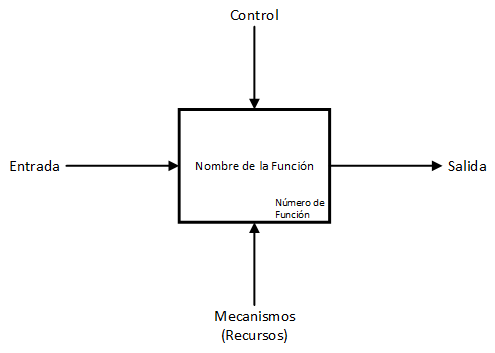
\includegraphics[scale=0.65]{marcoref/IDEFBlock}
	\caption{Bloque constructivo de un diagrama IDEF0.}
	\label{img:bloqueidef0}
\end{figure}

\noindent El bloque mostrado en la imagen \ref{img:bloqueidef0} tiene tres entradas y una salida. Estas entradas y salidas representan lo siguiente:

\begin{itemize}
	\item La se\~{n}al de entrada representa el recurso que ser\'a transformado en algo.
	\item La se\~{n}al de control representa todas aquellas variables o condiciones que dictan que la funci\'on deba realizarse.
	\item La se\~{n}al de mecanismos representa todas aquellas herramientas, t\'ecnicas, procesos, etc., que ayudan o son necesarios para la creaci\'on de la salida o transformaci\'on de la entrada.
	\item La se\~{n}al de salida representa el recurso obtenido de la funci\'on. Este recurso, al igual que las entradas, puede ser energ\'ia, informaci\'on o materia.
\end{itemize}

		\subsection{Diagrama de bloques mejorado de flujo de funciones} \label{subsec:effbd}
Los diagramas de bloques mejorados de flujo de funciones (\textit{enhanced Functional Flow Block Diagram}, eFFBD) son un medio de representaci\'on gr\'afica que describe el comportamiento de un sistema [?].\\

\noindent Esta herramienta describe el comportamiento de sistemas complejos, distribuidos, jer\'arquicos, concurrentes y comunicados. La representaci\'on eFFBD ofrece una gran variedad de estructuras de control como estructuras de iteraci\'on, paralelismo de funciones, ramas de decisi\'on, etc. La herramienta eFFBD ayuda a quienes la utilizan a entender el flujo de actividades, funciones y recursos de un sistema desde un punto de vista secuencial. Esta herramienta describe el funcionamiento del sistema a trav\'es del tiempo, de modo que el comportamiento puede ser entendido de inicio a fin. En la imagen \ref{img:diagramaeFFBD} se muestra un ejemplo de diagrama eFFBD.

\begin{figure}[H]
	\centering
		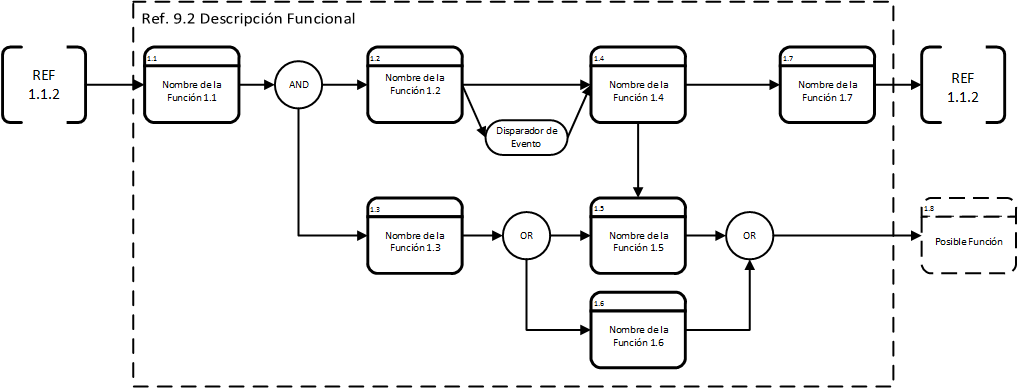
\includegraphics[scale=0.5]{marcoref/eFFBD}
	\caption{Diagrama eFFBD.}
	\label{img:diagramaeFFBD}
\end{figure}

En la imagen \ref{img:diagramaeFFBD} se puede observar que la primera funci\'on en ejecutarse es la funci\'on $1.1$. Al finalizar la funci\'on $1.1$, las funciones $1.2$ y $1.3$ comienzan a ejecutarse en paralelo. Al finalizar estos procesos, la funci\'on $1.4$ podr\'a ejecutarse en paralelo con la funci\'on $1.5$ o $1.6$, pero no con ambas a la vez. Una vez acabado este procedimiento, la funci\'on $1.7$ se ejecuta, y as\'i acaba el proceso completo.\\

\noindent Como se ha mencionado, el diagrama eFFBD permite entender el comportamiento del sistema a lo largo de su tiempo de ejecuci\'on (a diferencia del diagrama IDEF0 explicado en la secci\'on \ref{subsec:idef0}, que s\'olo muestra la relaci\'on que hay entre las funciones, m\'as no su ejecuci\'on a lo largo del tiempo).

		\subsection{Proceso de an\'alisis jer\'arquico} \label{subsec:ahp}
El proceso de an\'alisis jer\'arquico (\textit{Analytic Hierarchy Process}, AHP) es un m\'etodo de evaluaci\'on multicriterio desarrollado por Thomas L. Saaty que permite la jerarquizaci\'on de un proceso [?].\\

\noindent Tiene como fin el poder optimizar la toma de decisiones ante un problema complejo. Este m\'etodo es aplicado a la toma de decisiones en la que existen varias opciones y se debe elegir la m\'as adecuada con base en los criterios considerados. El m\'etodo de evaluaci\'on AHP contempla la experiencia del personal involucrado en la toma de la decisi\'on, junto con la informaci\'on cuantitativa del problema.\\

\noindent El m\'etodo AHP est\'a fundamentado en lo siguiente:

\begin{itemize}
	\item Toma de decisi\'on con base en los criterios planteados.
	\item Comparaciones por pares entre elementos con base en los criterios.
	\item Evaluaci\'on de los elementos mediante asignaciones de pesos.
	\item Priorizaci\'on de las alternativas de acuerdo a los pesos asignados.
\end{itemize}

%*************************************************************************************************************************************%	
	\section{Fundamentos del problema} \label{sec:basics}
		\subsection{CanSat} \label{subsec:cansat}
Un CanSat es una simulaci\'on de un sat\'elite real [?], pero con el tama\~{n}o de una lata de refresco\footnote{Las dimensiones del CanSat dise\~{n}ado en este trabajo corresponden a las especificadas por la competencia \textit{Annual CanSat Competition} y que son, por requerimiento, mayores a las de una lata de refresco.}.\\

\noindent Los CanSats son peque\~{n}os dispositivos compuestos por diferentes elementos mec\'anicos y electr\'onicos cuyo prop\'osito es simular una misi\'on de un sat\'elite de gran escala. Estos dispositivos son elevados unos cuantos cientos de metros para despu\'es ser liberados. Los CanSats pueden tener alg\'un medio de reducci\'on de velocidad (paraca\'idas, serpentinas, h\'elices, escudo de calor) o descender en ca\'ida libre. Durante todo el tiempo de vuelo los CanSats com\'unmente env\'ian datos de variables atmosf\'ericas como presi\'on atmosf\'erica, temperatura y humedad. Estos dispositivos pueden variar en especificaciones de acuerdo a la misi\'on, sin embargo, presentan siempre similitudes en cuanto a las tareas b\'asicas de telemetr\'ia.\\

\noindent Los CanSats son usados mayormente con prop\'ositos educativos y proveen a los estudiantes involucrados en su dise\~{n}o de m\'ultiples responsabilidades, que van desde la concepci\'on de la misi\'on, hasta la integraci\'on de los elementos. Estos dispositivos pretenden integrar m\'ultiples \'areas del conocimiento y encaminarlas a la gesti\'on de un proyecto de tipo aeroespacial.

		\subsection{Fen\'omeno de autorrotaci\'on} \label{subsec:autorot}
Las aereonaves de ala rotativa son aquellas en la que la fuerza de sustentaci\'on se logra mediante el giro de alas o palas, que forman parte del rotor, alrededor de un eje fijo. Las tres fuerzas principales que act\'uan sobre una pala del rotor son la fuerza de sustentaci\'on, $\overrightarrow{\text{dL}}$, la fuerza de arrastre, $\overrightarrow{\text{dD}}$, y la fuerza centr\'ifuga $\overrightarrow{\text{F}_\text{c}}$. La fuerza de sustentaci\'on es la fuerza hacia arriba causada por la interacci\'on entre el flujo de aire y el perfil aereodin\'amico. La fuerza de arrastre es quella que se opone al movimiento de la superficie de sustentaci\'on. La fuerza centr\'ifuga representa la tendencia de la pala del rotor a volar lejos del centro. Debido al movimiento circular, la velocidad del aire es mucho m\'as alta en la punta de la pala que en la base. La figura \ref{img:Helicoptero} muestra c\'omo act\'uan estas fuerzas en una aereonave de ala rotativa, en este caso, un helic\'optero.

\begin{figure}[H]
	\centering
		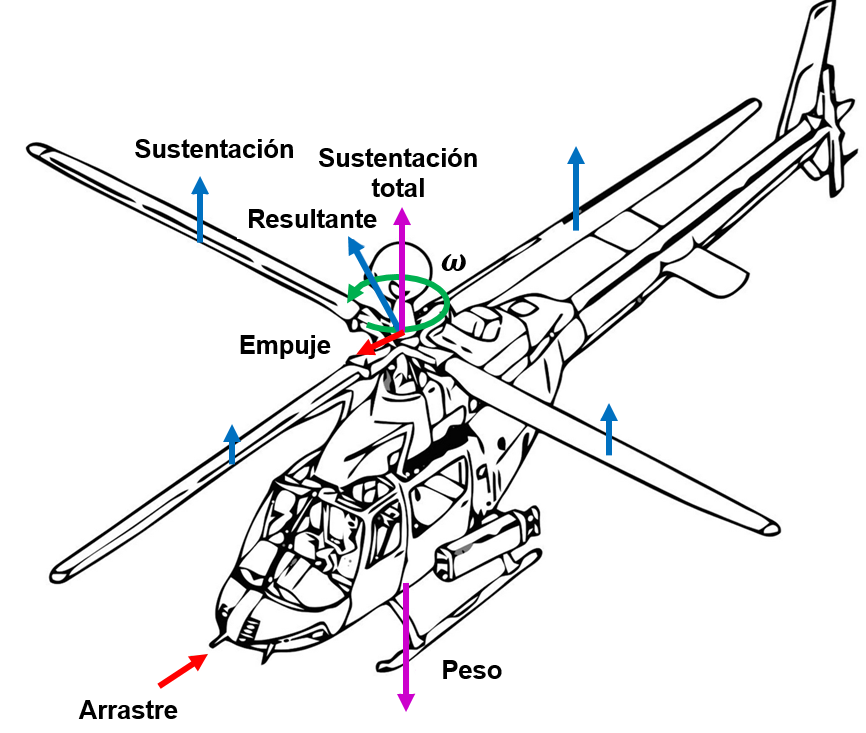
\includegraphics[scale=0.35]{imgmeca/Helicoptero.png}
	\caption{Fuerzas que act\'uan en el vuelo de una aereonave de ala rotativa.}
	\label{img:Helicoptero}
\end{figure}

\noindent La autorrotaci\'on  es un estado de vuelo que se presenta cuando el rotor principal de una aereonave de ala rotativa es movido por acci\'on del aire que va de abajo hacia arriba, y no precisamente por el motor o motores de la aereonave. En la autorrotaci\'on la corriente del aire entra desde la zona inferior del rotor y genera fuerzas aereodin\'amicas que lo mantienen en movimiento. Es el comportamiento habitual de los generadores e\'olicos, en los que el rotor extrae energ\'ia de la corriente de aire. Este fen\'omeno se muestra en la imagen \ref{img:Autorrotacion}.

\begin{figure}[H]
	\centering
		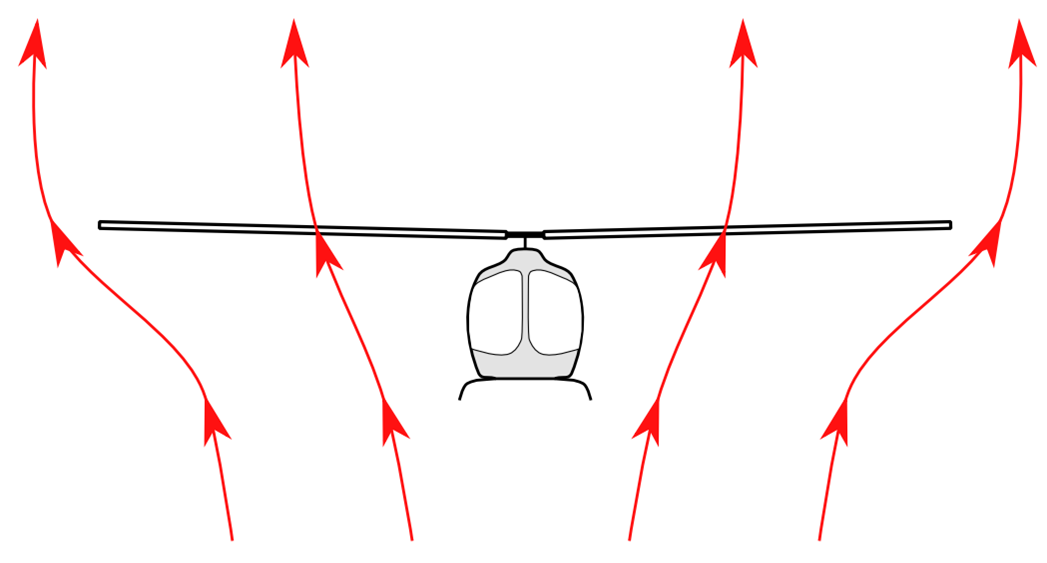
\includegraphics[scale=0.27]{imgmeca/Autorrotacion.png}
	\caption{Autorrotaci\'on. En rojo se muestran las l\'ineas de corriente con la direcci\'on de la velocidad de la corriente de aire.}
	\label{img:Autorrotacion}
\end{figure}


\noindent En este fen\'omeno la corriente de aire mantiene en movimiento a la aereonave de ala rotativa, ya que la sustentaci\'on es perpendicular a la corriente incidente y genera una fuerza que pone en movimiento las palas. Conforme vaya girando el rotor, el vector de fuerzas aereodin\'amicas de cada pala ir\'a girando hacia arriba, frenando la ca\'ida de la aereonave de ala rotativa.\\

En relaci\'on a la geometr\'ia de las palas \ref{}, los \'agulos de entrada de corriente son mayores en la zona de la ra\'iz de la pala, mientras que en  la punta son menores. Por lo tanto:

\begin{itemize}
\item Las zonas interiores de la pala presentan \'angulos de ataque grandes y la sustentaci\'on se orienta en la misma direcci\'on que la velocidad de rotaci\'on por lo que \'esta produce la potencia.
\item La zona de la punta de la pala presenta \'angulos de ataque peque\~{n}os y la sustentaci\'on se orienta en direcci\'on opuesta a la velocidad de rotaci\'on por lo que esta zona consume potencia.
\item En la condici\'on de autorrotaci\'on el par neto comunicado por esta confguraci\'on es nulo. La velocidad del rotor se ajustar\'a hasta alacanzar el equilibrio entre las fuerzas de inercia de rotaci\'on y las fuerzas aereodin\'amicas.
\end{itemize}
 
La figura \ref{img:Potencia} muestra las zonas productora y la zona consumidora de potencia durante la autorrotaci\'on.

\begin{figure}[H]
	\centering
	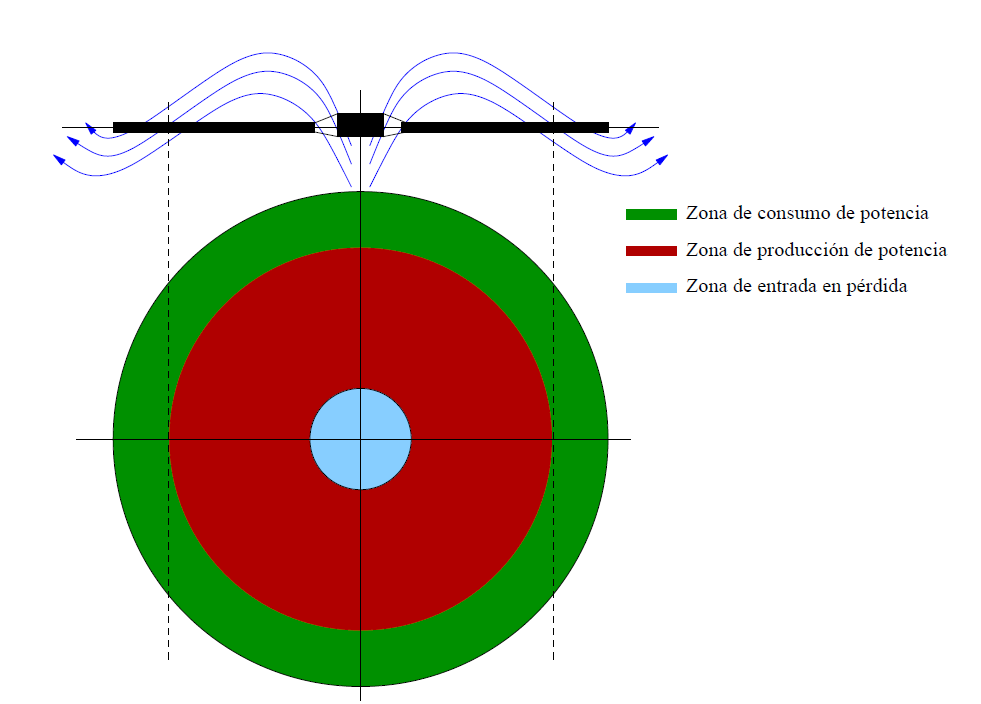
\includegraphics[scale=0.35]{imgmeca/Potencia.png}
	\caption{Zonas cosumidoras y productoras de potencia en el rotor durante el fen\'omeno de autorrotaci\'on.}
	\label{img:Potencia}
\end{figure}

\noindent Existe una zona en el rotor que ni consume ni genera potencia durante la autorrotaci\'on. En esta secci\'on las fuerzas tangenciales con nulas y s\'olo se produce el empuje. En la figura \ref{img:Secciones} la seccci\'on A corresponde con la caracter\'istica en autorrotaci\'on, la B como una secci\'on generadora de potencia y la C como una zona consumidora de potencia \ref{}.

\begin{figure}[H]
	\centering
	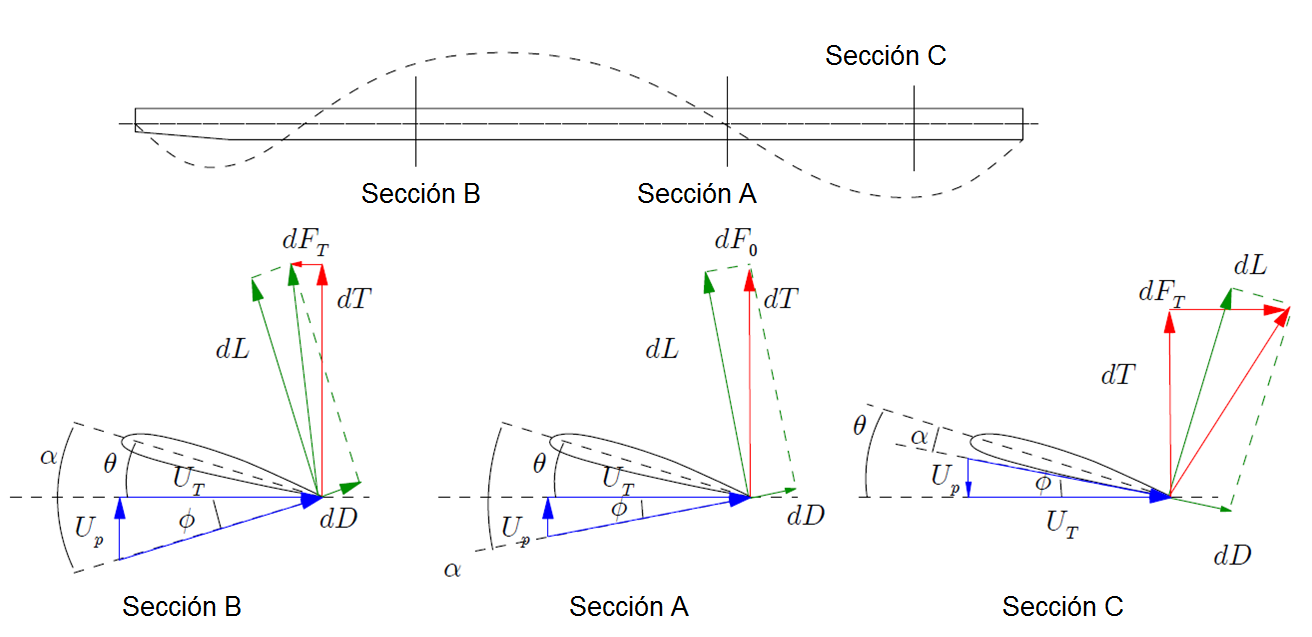
\includegraphics[scale=0.35]{imgmeca/Secciones.png}
	\caption{Secciones de h\'elice durante el fen\'omeno de autorrotaci\'on.}
	\label{img:Secciones}
\end{figure}

en donde $\text{dF}_{\text{T}}$ corresponde a la fuerza resultante entre la fuerza de arrastre y la fuerza de sustentaci\'on; $\text{U}_{p}$ y $\text{U}_{T}$ corresponden a los componenetes de la velocidad de viento perpendicular y tangencial, respectivamente; $\phi$ representa el \'angulo de entrada de corriente; $\theta$ es el \'angulo de paso y $\alpha$ es el \'angulo de ataque.

%%%%%%%%%%%%%%%%%%%%%%%%%%%%%%%%%%%%%%%%%%%%%%%%%%%%%%%%%%%%%%%%%%%
% !TeX encoding = ISO-8859-1
\chapter{Dise�o del sistema}

\begin{flushright}
\small\textit{Frase inspiradora dicha por alg�n personaje\\ del que CONOZCAMOS su trayectoria.}\\
		\small\textbf{Autor de la frase de arriba.}
\end{flushright}

% ******************************************************************************************************************************%
	\section{Dise�o preliminar}
		% !TeX encoding = ISO-8859-1
		\subsection{Necesidades y requerimientos}
			\subsubsection*{Necesidades}
La primera etapa en el proceso de dise�o es la identificaci�n de las necesidades, los problemas u oportunidades. Esta etapa permite encontrar una mejora o ventaja sobre alguna soluci�n ya existente a un problema, por lo que es posible reconocer el beneficio que traer� el llevar a cabo un proyecto.\\

\noindent Para el desarrollo de un CanSat las necesidades pueden variar dependiendo de la aplicaci�n que se le dar� al mismo, del lugar en donde ser� lanzado, de los recursos materiales, financieros y humanos disponibles, y de los alcances que se busquen.\\

\noindent En la Tabla \ref{tab:necesidades} se presentan las necesidades identificadas para el desarrollo del CanSat presentado en este trabajo. Es importante mencionar que las necesidades expuestas en la Tabla \ref{tab:necesidades} se originan de los requerimientos proporcionados por el concurso \textit{Annual CanSat Competition} para su edici�n 2019, por lo que no se realiz� ninguna investigaci�n previa para identificar dichas necesidades.\\

\begin{table}[H]
	\begin{center}
	\caption{Necesidades a satisfacer con el desarrollo del CanSat.}
	\label{tab:necesidades}
		\resizebox{14cm}{!}
		{
			\begin{tabular}{>{\centering}m{0.6cm} p{7.0cm} c p{0.6cm} p{7.0cm}}
			
\multicolumn{5}{c}{}\tabularnewline
\toprule
\multicolumn{2}{c}{\textbf{Funcionales}} &  &\multicolumn{2}{c}{\textbf{No funcionales}} 
\tabularnewline\hline\tabularnewline			

N01 & Medici�n y monitoreo de par�metros externos e internos. &  & N16 & Interfaz amena para el usuario.\tabularnewline

N02 & Poca masa. &  & N17 & Realizar una baja inversi�n para el desarrollo del proyecto.\tabularnewline

N03 & Dimensiones peque�as. &  & N18 & Reducir p�rdidas de energ�a por fricci�n entre partes m�viles. \tabularnewline

N04 & Poseer medios de reducci�n de velocidad de ca�da. &  & N19 &F�cil manufactura. \tabularnewline

N05 & Evitar atascamiento entre partes m�viles. &  & N20 &Poseer modos de operaci�n controlados por el usuario. \tabularnewline

N06 & Soportar fuerzas de impacto, aceleraciones y vibraciones. &  & N21 &Simplicidad al ensamblar y transportar. \tabularnewline

N07 & Capacidad de trabajo por horas. &  & N22 &Utilizar componentes comerciales y remplazables. \tabularnewline

N08 & Protecci�n contra el entorno. &  & N23 &F�cil acceso a los componenetes. \tabularnewline

N09 & Ser capaz de operar a temperaturas elevadas. &  & N24 &Poseer medios de localizaci�n. \tabularnewline

N10 & Asegurar integridad del sitio de lanzamiento. &  &  & \tabularnewline

N11 & La velocidad de descenso debe ser suave y debe estar acotada. &  & & \tabularnewline

N12 & Comunicaci�n continua de gran alcance. &  &  & \tabularnewline
 
N13 & Autonom�a completa en todos los componentes. & &  &\tabularnewline

N14 & Grabar etapas de vuelo. & &  &\tabularnewline

N15 & Almacenamiento constante de la informaci�n. & &  & \tabularnewline

\bottomrule			
			\end{tabular}
		}
	\end{center}
\end{table}

			\subsubsection*{Requerimientos}
La transformaci�n de las necesidades en un lenguaje t�cnico que permita materializar las posibles soluciones se logra por medio de la definici�n de los requerimientos.\\

\noindent Un requerimiento es una capacidad o atributo observable y medible de un sistema cuya finalidad es cumplir los objetivos de �ste. Un requerimiento debe ser necesario,  debe especificar qu� debe hacerse (y no c�mo hacerlo), debe abordar una s�la solicitud de manera completa y sin ambig�edades y, finalmente, debe ser realizable y verificable \cite{requirements_2017}.\\

\noindent Los requerimientos se pueden clasificar en requerimientos funcionales y no funcionales. Los requerimientos funcionales son aquellos que van enfocados a los aspectos t�cnicos  y que est�n relacionados con el funcionamiento del sistema. Por otro lado, los requerimientos no funcionales van dirigidos a aspectos est�ticos, por ejemplo, el color.\\
  
\noindent Para el desarrollo del Cansat se definieron los requerimientos funcionales mostrados en la Tabla \ref{tab:RequerimientosFun}. Cabe mencionar que los requerimientos definidos en la Tabla \ref{tab:RequerimientosFun} corresponden a los de la competencia \textit{Annual CanSat Competition}, con algunas modificaciones.

\begin{table}[H]
\begin{center}
\caption{Requerimientos funcionales del CanSat.}
\label{tab:RequerimientosFun}
\resizebox{13cm}{!}{
\begin{tabular}{>{\centering}m{1cm} p{13cm}}
\multicolumn{2}{c}{}\tabularnewline
\toprule

\multicolumn{1}{c}{\textbf{No.}} & \multicolumn{1}{c}{\textbf{Descripci�n}}
\tabularnewline
\hline
\tabularnewline

R01 & La masa total del CanSat deber� ser menor a $1 [kg]$. \tabularnewline

R02 & Las dimensiones m�ximas del CanSat deber�n ser $125 [mm]$ de di�metro por $310 [mm]$ de longitud.\tabularnewline

R03 & El CanSat deber� abrir el paraca�das del contenedor inmediatamente despu�s de ser liberado del veh�culo que lo eleve a la altura m�xima ($400 [m]$).\tabularnewline

R04 & La velocidad de descenso del CanSat (contenedor y veh�culo cient�fico) deber� ser de $20 [m/s]$ $\pm$ $5 [m/s]$ despu�s de ser liberado del veh�culo que lo elev�.\tabularnewline

R05 & El contenedor y el veh�culo cient�fico deber�n separarse a una altura de $300 [m]$ $\pm$ $10 [m]$ con respecto del sitio de lanzamiento.\tabularnewline 

R06 & El veh�culo cient�fico, despu�s de separarse del contenedor, deber� caer utilizando un sistema de descenso por autorrotaci�n.\tabularnewline

R07 & La velocidad de descenso del veh�culo cient�fico, despu�s de separarse del contenedor, deber� ser de $10$ $[m/s]$ a $15$ $[m/s]$.\tabularnewline

R08 & Todos los componentes de acoplamiento para el descenso del CanSat deber�n soportar fuerzas de hasta $30 [Gs]$.\tabularnewline

R09 & Todas las estructuras deber�n soportar hasta $15 [Gs]$ de aceleraci�n.\tabularnewline

R10 & Todos los componentes electr�nicos deber�n poseer una montura r�gida.\tabularnewline

R11 & Todos los mecanismos deber�n mantener sus respectivas configuraciones o estados bajo la acci�n de cualquier fuerza presente durante la etapa de vuelo.\tabularnewline

R12 & El veh�culo cient�fico deber� medir la altura con respecto al sitio de lanzamiento y la presi�n atmosf�rica.\tabularnewline

R13 & El veh�culo cient�fico deber� medir su posici�n global.\tabularnewline

% R14 & El veh�culo cient�fico deber� medir el nivel de tensi�n en las bater�as.\tabularnewline

R14 & El veh�culo cient�fico deber� medir la temperatura del ambiente.\tabularnewline

R15 & El veh�culo cient�fico deber� medir la velocidad de giro de las h�lices del sistema de descenso por autorrotaci�n relativa al veh�culo cient�fico.\tabularnewline

R16 & El veh�culo cient�fico deber� medir la inclinaci�n en los ejes \textit{pitch} y \textit{roll}.\tabularnewline

R17 & El veh�culo cient�fico deber� transmitir los datos de telemetr�a a una estaci�n en Tierra.\tabularnewline

R18 & La estaci�n en Tierra deber� estar compuesta de una computadora port�til con un m�nimo de dos horas de bater�a, un m�dulo xBee y una antena de mano.\tabularnewline

R19 & La estaci�n en Tierra deber� enviar comandos al veh�culo cient�fico para la calibraci�n de las referencias de altura e inclinaci�n (ejes \textit{pitch} y \textit{roll}).\tabularnewline

R20 & Deber� desarrollarse una interfaz de usuario para la estaci�n en Tierra.\tabularnewline

R21 & La interfaz de usuario deber� generar un archivo *\textit{.csv} con todos los datos de telemetr�a recibidos.\tabularnewline

\bottomrule
\end{tabular}
}
\end{center}
\end{table}

\begin{table}[H]
\ContinuedFloat
\begin{center}
\caption{Requerimientos funcionales del CanSat (continuaci�n).}
\resizebox{13cm}{!}{
\begin{tabular}{>{\centering}m{1cm} p{13cm}}
\multicolumn{2}{c}{}\tabularnewline
\toprule

\multicolumn{1}{c}{\textbf{No.}} & \multicolumn{1}{c}{\textbf{Descripci�n}}
\tabularnewline
\hline
\tabularnewline
R22 & Los datos de telemetr�a deber�n ser mostrados en la interfaz de usuario en unidades del Sistema Internacional.\tabularnewline

R23 & Se deber�n usar m�dulos xBee para la transmisi�n de datos de telemetr�a.\tabularnewline

R24 & La antena de la estaci�n en Tierra deber� recibir los datos de telemetr�a provenientes del CanSat sin importar la orientaci�n de �ste.\tabularnewline

R25 & La transmisi�n de datos de telemetr�a deber� tener un alcance m�nimo de $400 [m]$ en l�nea recta.\tabularnewline

R26 & Los datos de telemetr�a deber�n ser mostrados en tiempo real en la interfaz de usuario durante todo el tiempo de vuelo.\tabularnewline

R27 & Los datos de telemetr�a deber�n incluir el tiempo de misi�n con una resoluci�n de un segundo o mejor.\tabularnewline

R28 & La estaci�n en Tierra deber� ser port�til.\tabularnewline

R29 & El veh�culo cient�fico deber� mantener la cuenta de los paquetes de datos enviados.\tabularnewline

R30 & El veh�culo cient�fico deber� mantener la cuenta de los paquetes de datos enviados y del tiempo de misi�n a�n cuando suceda un reinicio inesperado.\tabularnewline

R31 & El veh�culo cient�fico deber� poseer un interruptor principal de f�cil acceso.\tabularnewline

R32 & El descenso por autorrotaci�n deber� ser pasivo.\tabularnewline

R33 & El CanSat deber� operar por un m�nimo de dos horas.\tabularnewline

R34 & El CanSat deber� operar adecuadamente durante las pruebas ambientales de dimensiones, vibraciones, temperatura y ca�da.\tabularnewline

R35 & El CanSat deber� registrar todo el vuelo utilizando una c�mara.\tabularnewline

R36 & La c�mara deber� estar alineada con respecto al campo magn�tico de la Tierra en una orientaci�n aleatoria.\tabularnewline

R37 & La c�mara deber� estar a $45^o$ con respecto del nadir.\tabularnewline

R38 & El CanSat deber� tener un modo de operaci�n autom�tico y un modo de operaci�n manual.\tabularnewline

R39 & El veh�culo cient�fico deber� poseer un indicador auditivo con un nivel de presi�n de sonido de $92 [dB]$.\tabularnewline

\bottomrule
\end{tabular}
}
\end{center}
\end{table}

\noindent A continuaci�n, se enlistan los requerimientos no funcionales considerados para el desarrollo del CanSat. Estos requerimientos no afectan el desempe�o del CanSat durante el desarrollo de la misi�n.

\begin{itemize}
	\item El contenedor deber� ser de alg�n color fluorescente (rosa, rojo o amarillo).
	\item Los mecanismos que utilicen calor (en caso de haber) no deber�n ser expuestos al exterior.
	\item El veh�culo cient�fico deber� poseer un indicador LED de encendido de f�cil visualizaci�n.
	\item El paraca�das del contenedor deber� ser de color fluorescente (rosa o naranja).
\end{itemize}

		\subsection{Definici�n de la actividad del usuario}
Un modo de operaci�n se define como una capacidad operativa distinta del sistema: esta capacidad operativa puede usar el conjunto completo de las funciones del sistema o s�lo una parte \cite{operationmodes_1992}. Tener distintos modos de operaci�n permite un mejor aprovechamiento de los recursos energ�ticos ya que los modos de operaci�n agrupan s�lo las funciones necesarias para la situaci�n actual del sistema, o las activan s�lo cuando es necesario. A continuaci�n, se enlistan los dos modos de operaci�n del CanSat.

\begin{itemize}
	\item \textbf{Modo autom�tico: } El CanSat mide par�metros del entorno, los almacena en la memoria de abordo y los transmite a la estaci�n en Tierra. Toma decisiones con base en dichos par�metros para realizar las operaciones de la misi�n de vuelo. En la estaci�n en Tierra se despliegan los par�metros recibidos y se almacenan en un archivo. El CanSat tendr� este modo de operaci�n al momento de su lanzamiento.
	\item \textbf{Modo manual: } El CanSat mide par�metros del entorno, los almacena en la memoria de abordo y los transmite a la estaci�n en Tierra. El usuario tiene control sobre el comportamiento del sistema. La estaci�n en Tierra muestra en pantalla los par�metros recibidos y los almacena en un archivo. El CanSat tendr� este modo de operaci�n durante la demostraci�n de su funcionamiento en Tierra.
\end{itemize}

		\subsection{Desarrollo de las arquitecturas del sistema}
			\subsubsection{Arquitectura funcional}
De acuerdo con \cite{engineeringdesign_2007}, una funci�n es un proceso que toma entradas y las transforma en salidas. Para el desarrollo del CanSat se sigui� una metodolog�a con enfoque funcional, por lo tanto, se defini� la lista de funciones que realiza el sistema (FBS). Agregado a esta lista, se desarrollaron diagramas IDEF0 y eFFBD que muestran las relaciones que hay entre las funciones y c�mo �stas describen el comportamiento del sistema; en concreto, se desarroll� la arquitectura funcional del sistema (\textit{System Functional Architecture}, SFA). \\

\noindent Para la realizaci�n de la descomposici�n FBS se tom� como referencia el conjunto de funciones gen�ricas propuesto por Flores Hern�ndez \cite{diegoflores_2018} donde especifica que todo sistema mecatr�nico debe tener las siguientes funciones:

\begin{itemize}
	\item Medici�n de par�metros ambientales y del sistema.
	\item Detecci�n de errores del sistema.
	\item Interacci�n con el usuario.
	\item Gesti�n de las decisiones.
	\item Acondicionamiento de las entradas y salidas del sistema.
	\item Almacenamiento de informaci�n.
	\item Comunicaci�n interna y externa.
	\item Recuperaci�n de las funcionalidades del sistema.
	\item Realizar las funciones particulares del sistema.
	\item Proteger y soportar.
	\item Gestionar energ�a.
\end{itemize}

\noindent Con base en esta estructura gen�rica, la Tabla \ref{tab:Funciones} muestra la descomposici�n FBS del CanSat. En la definici�n de las funciones se debe tener en cuenta que cada requerimiento debe estar asociado con al menos una funci�n, puesto que cada funci�n debe estar justificada.\\

\begin{table}[H]
\begin{center}
\caption{Descomposici�n de funciones del CanSat.}
\label{tab:Funciones}
\resizebox{13cm}{!}{ 
\begin{tabular}{lllcc}
\multicolumn{5}{c}{}\tabularnewline
\toprule 

\multicolumn{5}{c}{\textbf{CanSat con sistema de descenso por autorrotaci�n}}
\tabularnewline
\hline
\tabularnewline


1.0 & \multicolumn{4}{l}{Gestionar energ�a}\tabularnewline
 & 1.1 & \multicolumn{3}{l}{Acondicionar energ�a}\tabularnewline
 & 1.2 & \multicolumn{3}{l}{Distribuir energ�a}\tabularnewline
 & 1.3 & \multicolumn{3}{l}{Almacenar energ�a}\tabularnewline
2.0 & \multicolumn{4}{l}{Gestionar informaci�n}\tabularnewline
 & 2.1 & \multicolumn{3}{l}{Administrar datos}\tabularnewline
 &  & 2.1.1 & \multicolumn{2}{l}{Comunicar internamente}\tabularnewline
 &  & 2.1.2 & \multicolumn{2}{l}{Almacenar datos}\tabularnewline
 &  & 2.1.3 & \multicolumn{2}{l}{Procesar datos}\tabularnewline
 &  & 2.1.4 & \multicolumn{2}{l}{Interactuar con el usuario}\tabularnewline
 & 2.2 & \multicolumn{3}{l}{Medir par�metros}\tabularnewline
 &  & 2.2.1 & \multicolumn{2}{l}{Medir par�metros internos}\tabularnewline 
 &  &  & 2.2.1.1 & \multicolumn{1}{l}{Medir hora y fecha}\tabularnewline
 &  &  & 2.2.1.2 & \multicolumn{1}{l}{Medir nivel de tensi�n en bater�as}\tabularnewline
  &  &  & 2.2.1.3 & \multicolumn{1}{l}{Medir velocidad angular}\tabularnewline
    &  &  & 2.2.1.4 & \multicolumn{1}{l}{Realizar conteo del n�mero de paquetes enviados}\tabularnewline
 &  &  2.2.2 & \multicolumn{2}{l}{Medir par�metros externos}\tabularnewline  
 &  &  & 2.2.2.1 & \multicolumn{1}{l}{Medir temperatura}\tabularnewline
 &  &  & 2.2.2.2 & \multicolumn{1}{l}{Medir presi�n barom�trica}\tabularnewline


\bottomrule
\end{tabular}
}
\end{center}
\end{table}

\begin{table}[H]
\ContinuedFloat
\begin{center}
\caption{Descomposici�n de funciones del CanSat (continuaci�n).}
\resizebox{13cm}{!}{ 
\begin{tabular}{lllcc}
\multicolumn{5}{c}{}\tabularnewline
\toprule 

\multicolumn{5}{c}{\textbf{CanSat con sistema de descenso por autorrotaci�n}}
\tabularnewline
\hline
\tabularnewline


  &  &  & 2.2.2.3 & \multicolumn{1}{l}{Medir componentes de gravedad en un sistema}\tabularnewline
  &  &  &  & \multicolumn{1}{l}{ de referencia cartesiano fijo}\tabularnewline  
  &  &  & 2.2.2.4 & \multicolumn{1}{l}{Medir velocidades angulares alrededor de los ejes de}\tabularnewline  
  &  &  &  & \multicolumn{1}{l}{un sistema de referencia cartesiano fijo}\tabularnewline     
  &  &  & 2.2.2.5 & \multicolumn{1}{l}{Medir componentes del campo magn�tico de la Tierra}\tabularnewline  
  &  &  & 2.2.2.6 & \multicolumn{1}{l}{Medir latitud, longitud y altitud}\tabularnewline  
 & 2.3 & \multicolumn{3}{l}{Tomar decisiones}\tabularnewline
 &  &  2.3.1 & \multicolumn{2}{l}{Recuperar funcionalidades}\tabularnewline
  &  &  2.3.2 & \multicolumn{2}{l}{Secuenciar comportamiento}\tabularnewline  
3.0 & \multicolumn{4}{l}{Proteger y soportar el sistema}\tabularnewline
4.0 & \multicolumn{4}{l}{Simular misi�n de vuelo}\tabularnewline
 & 4.1 & \multicolumn{3}{l}{Registrar descenso}\tabularnewline
 & & 4.1.1 & \multicolumn{2}{l}{Grabar evidencia de descenso}\tabularnewline 
  & & 4.1.2 & \multicolumn{2}{l}{Orientar c�mara}\tabularnewline  
 & 4.2 & \multicolumn{3}{l}{Comunicar con estaci�n en Tierra}\tabularnewline
  & 4.3 & \multicolumn{3}{l}{Reducir velocidad de descenso}\tabularnewline
 & 4.4 & \multicolumn{3}{l}{Orientar CanSat}\tabularnewline
  & 4.5 & \multicolumn{3}{l}{Liberar veh�culo cient�fico}\tabularnewline


\bottomrule
\end{tabular}
}
\end{center}
\end{table}

\noindent Los diagramas IDEF0 se usaron como una t�cnica de modelado gr�fica para representar las relaciones que hay entre las funciones dentro de cada nivel de la descomposici�n FBS. La imagen \ref{img:nodoA0} muestra el diagrama IDEF0 del nivel de mayor jerarqu�a de la descomposici�n de funciones del CanSat. La �nica entrada transformada por el CanSat es el conjunto de par�metros de inter�s que se miden a lo largo de la misi�n. Estos par�metros son transformados en datos mostrados en la interfaz de usuario, datos almacenados abordo del CanSat y en la estaci�n en Tierra, en un video grabado por la c�mara, y en un contenedor y veh�culo cient�fico separados.\\

\noindent El �ltimo de los elementos que componen a la arquitectura funcional son los diagramas eFFBD. La imagen \ref{img:eFFBDCanSat} muestra el diagrama eFFBD del CanSat en su modo de operaci�n autom�tico. En la imagen \ref{img:eFFBDCanSat} se puede ver que el CanSat gestiona la energ�a y le da soporte y protecci�n a todos los componentes durante toda la misi�n. Las dos funciones anteriores las realiza en paralelo con la gesti�n de la informaci�n y la simulaci�n de la misi�n de vuelo. Para la funci�n de gestionar informaci�n, el CanSat debe medir y procesar los datos antes de tomar decisiones con base en ellos. El CanSat debe primero calcular la altura, tomar la decisi�n de liberar al veh�culo cient�fico con base en el valor de altura obtenido y, finalmente, transmitir este dato, junto con los dem�s, a la estaci�n en Tierra.\\

\begin{figure}[H]
	\centering
		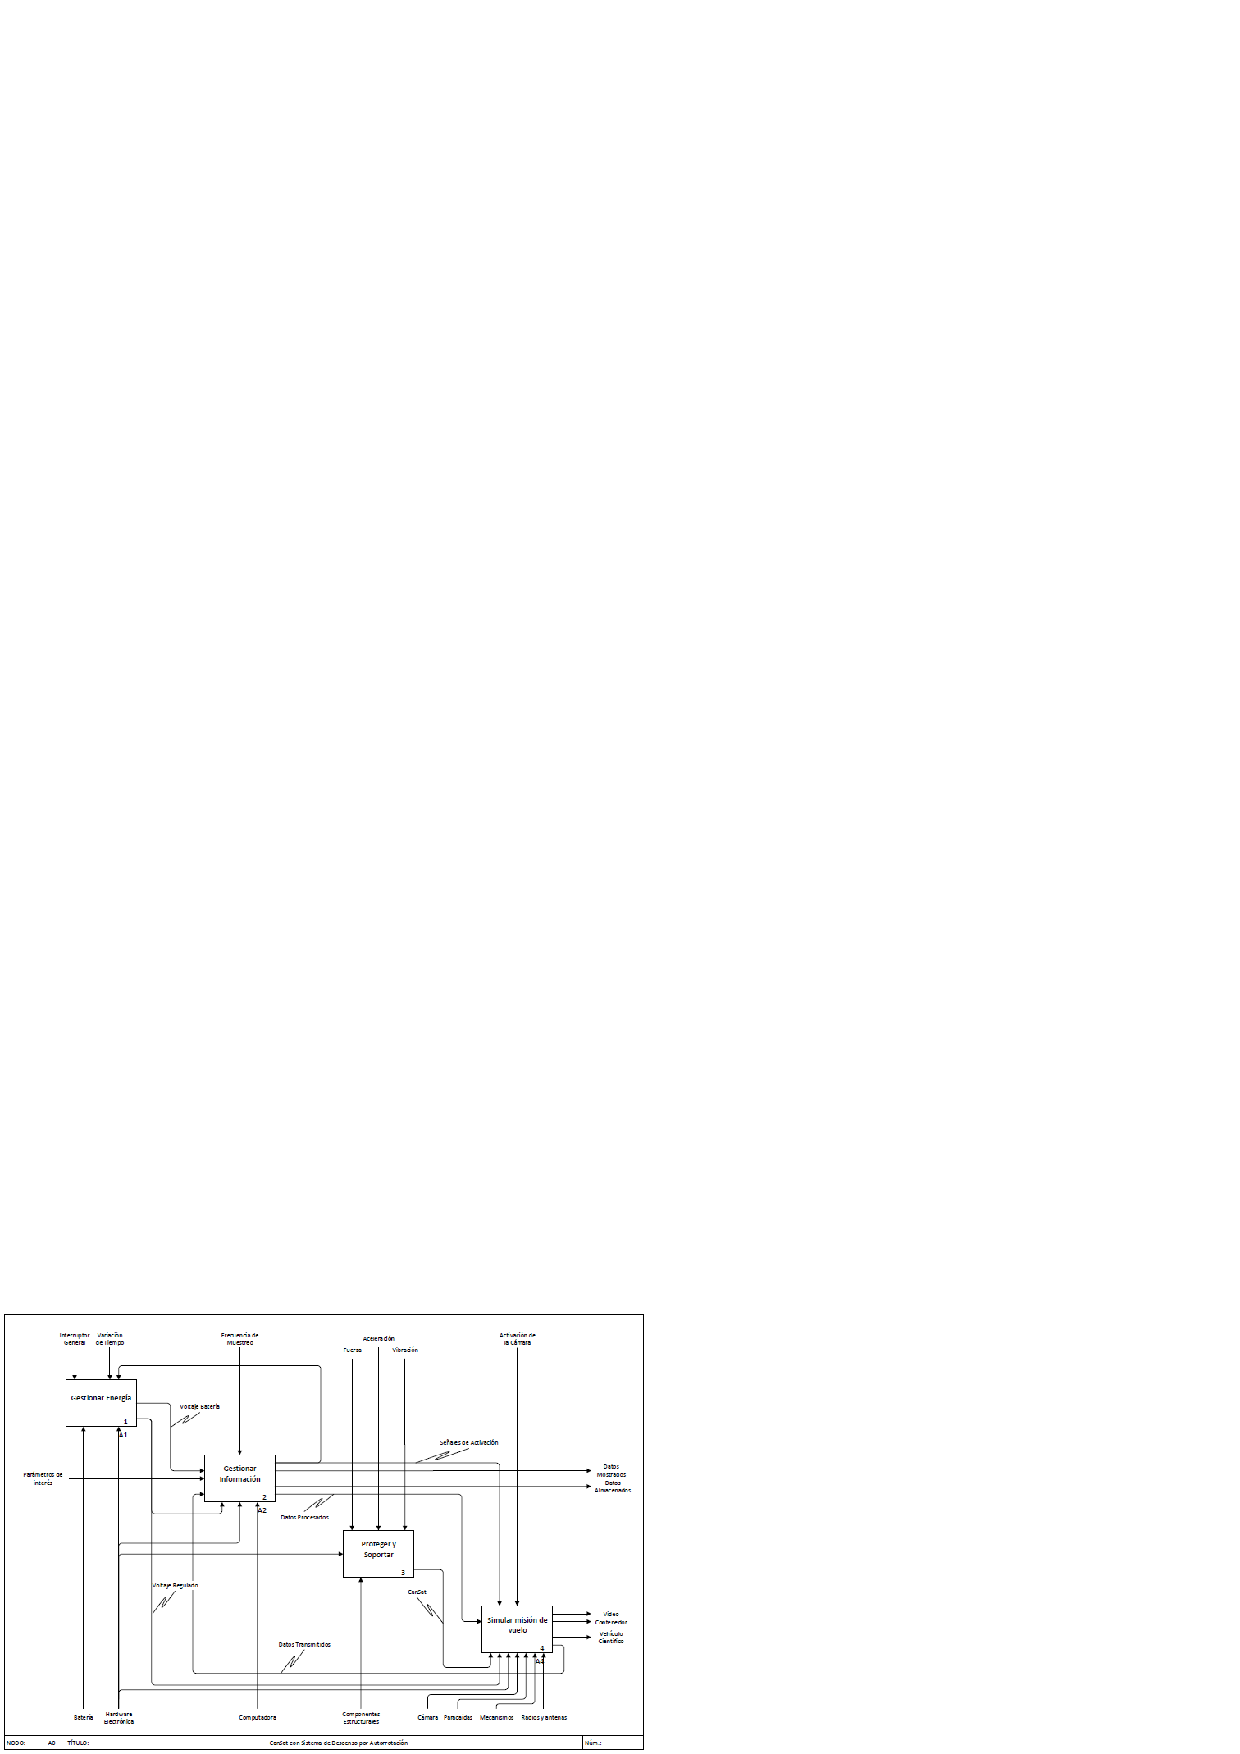
\includegraphics[scale=1.1]{diseniosist/IDEF0A0}
	\caption{Nodo A0 del diagrama IDEF0. CanSat con sistema de descenso por autorrotaci�n.}
	\label{img:nodoA0}
\end{figure}

\begin{figure}[H]
	\centering
		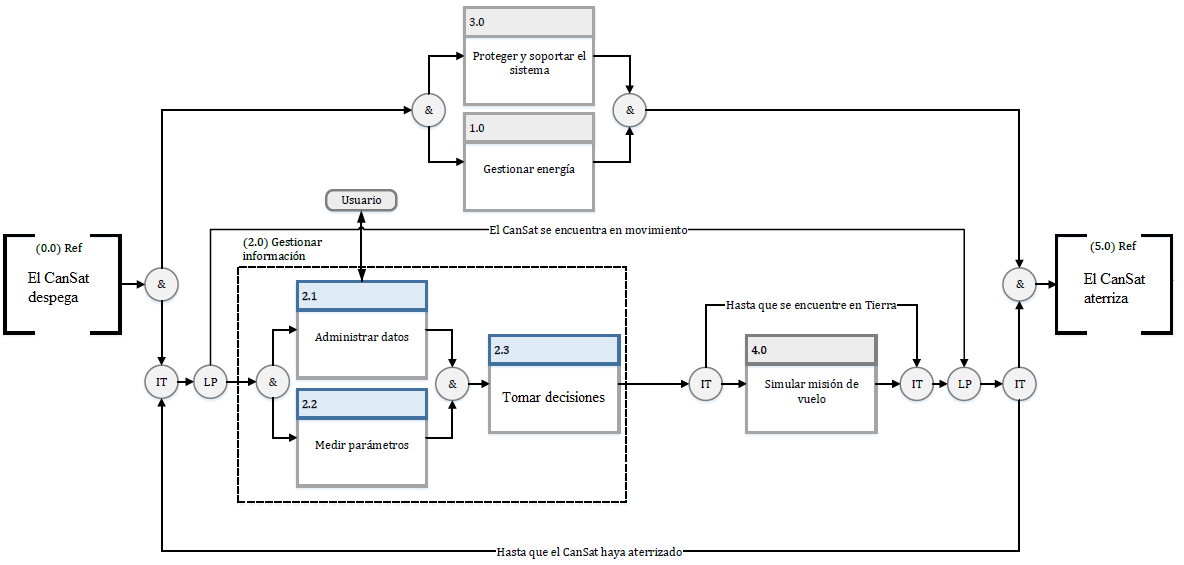
\includegraphics[scale=0.50]{diseniosist/eFFBDCanSat}
	\caption{Diagrama eFFBD del CanSat en modo autom�tico.}
	\label{img:eFFBDCanSat}
\end{figure}

\newpage
			\subsubsection*{Priorizaci�n de funciones}
\noindent Priorizar funciones tiene que ver con determinar qu� funci�n es la m�s importante de toda la descomposici�n FBS. En \cite{diegoflores_2018} se menciona que realizar este proceso de priorizaci�n permite al equipo de dise�o saber qu� funci�n afecta en mayor medida al comportamiento global del sistema, para despu�s poder aplicar t�cnicas de optimizaci�n a esa funci�n en particular, en lugar de optimizar todas y cada una de ellas.\\

\noindent El problema de priorizaci�n de funciones puede verse como un problema de toma de decisiones multicriterio que, como su nombre lo indica, se trata de tomar una decisi�n con base en varios criterios, donde cada uno tiene una influencia diferente en la toma de la decisi�n final. Al final de este proceso de toma de decisi�n multicriterio se puede saber cu�l de las opciones es la mejor, o vi�ndolo desde el punto de vista de priorizaci�n, qu� funci�n es la m�s importante. Para la priorizaci�n de funciones se utiliz� el m�todo AHP descrito en la secci�n \ref{sec:tools}. Para la realizaci�n de la priorizaci�n de funciones se tomaron en cuenta los criterios enlistados a continuaci�n.

\begin{itemize}
	\item \textbf{Importancia:} Hace referencia a si la funci�n evaluada es necesaria o si se trata de una funci�n complementaria. Durante el proceso de comparaci�n se puede responder a la siguiente pregunta: �es esta funci�n m�s importante que la otra para el comportamiento general del sistema?
	\item \textbf{Eficiencia:} Se refiere a qu� tanto ayuda una funci�n con respecto de la otra para el cumplimiento de los objetivos de dise�o y el comportamiento deseado. Para evaluar las funciones bajo este criterio puede hacerse la siguiente pregunta: �esta funci�n ayuda m�s que la otra para un mejor cumplimiento del comportamiento general del sistema?
	\item \textbf{Dependencia:} Se refiere a si la funci�n depende de otra(s) para ejecutarse. Al comparar dos funciones puede responderse a la siguiente pregunta: �esta funci�n depende de la otra para ejecutarse?
\end{itemize}

\noindent En el m�todo AHP primero se determina un vector de priorizaci�n de criterios $w_{cr}$ el cual indica el grado de influencia que cada criterio tiene durante el proceso de priorizaci�n. Posteriormente, se debe realizar una comparaci�n de cada funci�n contra cada funci�n (una tabla de comparaci�n de 26x26 en este caso) con respecto de cada criterio, respondiendo a la pregunta respectiva. Los resultados de esta comparaci�n por pares constituyen una matriz $MCR_{f}$ de 26x3. El vector de priorizaci�n de funciones $P_{f}$, tomando en cuenta todos los criterios y su respectivo grado de influencia en la decisi�n final, se obtiene al calcular $P_{f} = MCR_f \cdot w_{cr}$.\\

\noindent La Tabla \ref{tab:priorizacion de funciones} muestra el vector de priorizaci�n de funciones $P_{f}$ con base en la descomposici�n FBS de la tabla \ref{tab:Funciones}. En la Tabla \ref{tab:priorizacion de funciones} se observa que la funci�n $sf_{4\text{.}3}-$ \textit{Reducir velocidad de descenso} es la m�s importante, seguido de las funciones $sf_{3\text{.}0}-$ \textit{Proteger y soportar} y $sf_{1\text{.}1}-$\textit{Acondicionar energ�a}.\\

\begin{table}[H]
\begin{center}
\caption{Resultados del proceso de priorizaci�n de funciones.}
\label{tab:priorizacion de funciones}
\resizebox{13cm}{!}{
\begin{tabular}{p{8cm}p{2cm}p{2cm}p{2cm}}

\multicolumn{4}{c}{}\tabularnewline
\toprule
\textbf{Funci�n} & \textbf{No.} & \textbf{Posici�n} & \textbf{Valor}
\tabularnewline
\hline
\tabularnewline
  
Gestionar energ�a & $f_{1\text{.}0}$ & -- & --\tabularnewline
\rowcolor{lightgray}\;\;\;Acondicionar energ�a & $sf_{1\text{.}1}$ & \textbf{3} & 0.0679\tabularnewline
\;\;\;Distribuir energ�a & $sf_{1\text{.}2}$ & 8 & 0.0443\tabularnewline
\;\;\;Almacenar energ�a & $sf_{1\text{.}3}$ & 12 & 0.0408\tabularnewline

Gestionar informaci�n & $f_{2\text{.}0}$ & -- & --\tabularnewline

\;\;\;Administrar datos & $sf_{2\text{.}1}$ & -- & --\tabularnewline
\;\;\;\;\;\;Comunicar internamente & $sf_{2\text{.}1\text{.}1}$ & 5 & 0.0554\tabularnewline
\;\;\;\;\;\;Almacenar datos & $sf_{2\text{.}1\text{.}2}$ & 25 & 0.0220\tabularnewline
\;\;\;\;\;\;Procesar datos & $sf_{2\text{.}1\text{.}3}$ & 10 & 0.0413\tabularnewline
\;\;\;\;\;\;Interactuar con el usuario & $sf_{2\text{.}1\text{.}4}$ & 13 & 0.0398\tabularnewline

\;\;\;Medir par�metros & $sf_{2\text{.}2}$ & -- & --\tabularnewline
\;\;\;\;\;\;Medir par�metros internos & $sf_{2\text{.}2\text{.}1}$ & -- & --\tabularnewline
\;\;\;\;\;\;\;\;\;Medir hora y fecha & $sf_{2\text{.}2\text{.}1\text{.}1}$ & 18 & 0.0251\tabularnewline
\;\;\;\;\;\;\;\;\;Medir nivel de tensi�n en bater�as & $sf_{2\text{.}2\text{.}1\text{.}2}$ & 17 & 0.0251\tabularnewline
\;\;\;\;\;\;\;\;\;Medir velocidad angular & $sf_{2\text{.}2\text{.}1\text{.}3}$ & 11 &0.0411\tabularnewline
\;\;\;\;\;\;\;\;\;Realizar conteo del n�mero de paquetes & $sf_{2\text{.}2\text{.}1\text{.}4}$ & 16 & 0.0253\tabularnewline

\;\;\;\;\;\;Medir par�metros externos & $sf_{2\text{.}2\text{.}2}$ & -- & --\tabularnewline
\;\;\;\;\;\;\;\;\;Medir temperatura & $sf_{2\text{.}2\text{.}2\text{.}1}$ & 23 & 0.0245\tabularnewline
\;\;\;\;\;\;\;\;\;Medir presi�n barom�trica & $sf_{2\text{.}2\text{.}2\text{.}2}$ & 22 & 0.0245\tabularnewline
\;\;\;\;\;\;\;\;\;Medir componentes de gravedad en& $sf_{2\text{.}2\text{.}2\text{.}3}$ & 21 & 0.0248\tabularnewline
\;\;\;\;\;\;\;\;\;un sistema de referencia cartesiano fijo& & &\tabularnewline
\;\;\;\;\;\;\;\;\;Medir velocidades angulares alrededor de & $sf_{2\text{.}2\text{.}2\text{.}4}$ & 20 & 0.0248\tabularnewline
\;\;\;\;\;\;\;\;\;los ejes de un sistema de referencia& & &\tabularnewline
\;\;\;\;\;\;\;\;\;cartesiano fijo& & &\tabularnewline
\;\;\;\;\;\;\;\;\;Medir componentes del campo magn�tico & $sf_{2\text{.}2\text{.}2\text{.}5}$ & 19 & 0.0248\tabularnewline
\;\;\;\;\;\;\;\;\;de la Tierra& & &\tabularnewline
\;\;\;\;\;\;\;\;\;Medir latitud, longitud y altitud & $sf_{2\text{.}2\text{.}2\text{.}6}$ & 24 & 0.0244\tabularnewline

\;\;\;Tomar decisiones & $sf_{2\text{.}3}$ & -- & --\tabularnewline
\;\;\;\;\;\;Recuperar funcionalidades & $sf_{2\text{.}3\text{.}1}$ & 7 & 0.0478\tabularnewline
\;\;\;\;\;\;Secuenciar comportamiento & $sf_{2\text{.}3\text{.}2}$ & 6 & 0.0488\tabularnewline

\rowcolor{lightgray}Proteger y soportar el sistema & $f_{3\text{.}0}$ & \textbf{2} & 0.0703\tabularnewline

Simular misi�n de vuelo & $f_{4\text{.}0}$ & -- & --\tabularnewline
\;\;\;Registrar descenso & $sf_{4\text{.}1}$ & -- & --\tabularnewline
\;\;\;\;\;\;Grabar evidencia de descenso & $sf_{4\text{.}1\text{.}1}$ & 26 & 0.0192\tabularnewline
\;\;\;\;\;\;Orientar c�mara & $sf_{4\text{.}1\text{.}2}$ & 14 & 0.0294\tabularnewline
\;\;\;Comunicar con estaci�n en Tierra & $sf_{4\text{.}2}$ & 9 & 0.0415\tabularnewline
\rowcolor{lightgray}\;\;\;Reducir velocidad de descenso & $sf_{4\text{.}3}$ & \textbf{1} & 0.0742\tabularnewline
\;\;\;Orientar CanSat & $sf_{4\text{.}4}$ & 4 & 0.0638\tabularnewline
\;\;\;Liberar veh�culo cient�fico & $sf_{4\text{.}5}$ & 15 & 0.0291\tabularnewline
 
\bottomrule
\end{tabular}
}
\end{center}
\end{table}

\newpage

			\subsubsection{Arquitectura f�sica}
La arquitectura f�sica del sistema (\textit{System Physical Architecture}, SPA) se define como el conjunto de todas las transformaciones de funciones y subfunciones en sistemas, subsistemas, ensambles y componentes f�sicos \cite{engineeringdesign_2007}. Estos elementos deben cumplir con las funciones definidas previamente con el fin de otorgar el comportamiento deseado.\\

\noindent Al igual que con la arquitectura funcional, en \cite{diegoflores_2018} se propone una arquitectura f�sica gen�rica para cualquier sistema mecatr�nico que se compone de los siguientes sistemas:

\begin{itemize}
	\item Sistema Central de Manejo del Comportamiento.
	\item Sistema de Procesamiento de Datos.
	\item Sistema de Energ�a.
	\item Sistema Estructural.
	\item Sistemas propios del sistema mecatr�nico dise�ado.
\end{itemize}

\noindent La arquitectura f�sica del CanSat est� basada en la arquitectura gen�rica presentada anteriormente tal como se muestra en la figura \ref{img:SPACanSat}. La Tabla \ref{tab:sistemas y subsistemas} muestra la descripci�n de los sistemas y subsistemas del CanSat.

\begin{figure}[H]
	\centering
		\includegraphics[scale=0.85]{diseniosist/DiagramaArquitecturaFisica}
	\caption{Arquitectura f�sica del CanSat.}
	\label{img:SPACanSat}
\end{figure}


\begin{table}[H]
\begin{center}
\caption{Sistemas y subsistemas del CanSat.}
\label{tab:sistemas y subsistemas}
\resizebox{14cm}{!}{
\begin{tabular}{p{4cm}p{12cm}}
\multicolumn{2}{c}{}\tabularnewline
\toprule

\multicolumn{1}{c}{\textbf{Sistema}} & \multicolumn{1}{c}{\textbf{Descripci�n}}
\tabularnewline
\hline
\tabularnewline

($S_{1}$) Sistema Central de Manejo del Comportamiento (SCMC) & Este sistema est� encargado de determinar el comportamiento del CanSat de acuerdo con la etapa de vuelo en la que se encuentre. este sistema est� compuesto por dos subsistemas: el subsistema de percepci�n ($sS_{1\text{.}1}$ -- SP) encargado de la adquisici�n de los par�metros del entorno e internos; y el subsistema de toma de decisiones ($sS_{1\text{.}2}$ -- STD) encargado de habilitar o deshabilitar ciertas funciones del CanSat con base en los datos procesados.\tabularnewline\tabularnewline

($S_{2}$) Sistema de Procesamiento de Datos (SPD) & Este sistema est� encargado de procesar la informaci�n del entorno. El SPD est� formado por tres subsistemas: el subsistema de acondicionamiento de datos ($sS_{2\text{.}1}$ -- SAcD) que procesa los datos de los sensores; el subsistema de almacenamiento de datos ($sS_{2\text{.}2}$ -- SAlD) que almacena la informaci�n abordo; y el subsistema de comunicaci�n interna ($sS_{2\text{.}3}$ -- SCI), que distribuye la informaci�n a los componentes que la requieran.\tabularnewline\tabularnewline

($S_{3}$) Sistema de Reducci�n de Velocidad de Descenso (SRVD) & Este sistema se encarga de mantener la velocidad de descenso del CanSat dentro de los rangos establecidos en los requerimientos. El SRVD est� compuesto por dos subsistemas: el subsistema de reducci�n de velocidad por paraca�das ($sS_{3\text{.}1}$ -- SRV-P) cuya funci�n es mantener la velocidad de descenso de todo el CanSat dentro del rango de $15 [m/s]$ a $25 [m/s]$ antes de los $300 [m]$; y el subsistema de reducci�n de velocidad por autorrotaci�n ($sS_{3\text{.}2}$ -- SRV-A) cuya funci�n es mantener la velocidad de descenso del veh�culo cient�fico dentro del rango de $10 [m/s]$ a $15 [m/s]$.\tabularnewline\tabularnewline

($S_{4}$) Sistema de Liberaci�n del Veh�culo Cient�fico (SLVC) & Este sistema est� encargado de liberar al veh�culo cient�fico del contenedor a una altura de $300 [m]$.\tabularnewline\tabularnewline

($S_{5}$) Sistema de Registro de Descenso (SRD) & Este sistema se encarga de tomar evidencia en video a lo largo de toda la misi�n, enfocando siempre en la misma direcci�n con respecto del nadir.\tabularnewline\tabularnewline

($S_{6}$) Sistema de Estaci�n en Tierra (SET) & Este sistema se encarga de comunicar el CanSat con la estaci�n en Tierra y comunicar la estaci�n en Tierra con el usuario. El SET est� compuesto por dos subsistemas: el subsistema de comunicaci�n CanSat -- Estaci�n en Tierra ($sS_{6\text{.}1}$ -- SC-ET) cuya funci�n es transmitir informaci�n del CanSat a la estaci�n en Tierra y viceversa; y el subsistema de comunicaci�n Usuario -- Estaci�n en Tierra ($sS_{6\text{.}2}$ -- SU-ET) cuya funci�n es mostrar al usuario de forma amena la informaci�n que el CanSat env�e a la estaci�n en Tierra y crear un respaldo de esta informaci�n.\tabularnewline\tabularnewline

($S_{7}$) Sistema de Energ�a (SEn) & Este sistema est� encargado de gestionar la energ�a de consumo del CanSat. Realiza las funciones de almacenamiento, acondicionamiento y distribuci�n de la energ�a a todo el CanSat.\tabularnewline\tabularnewline

($S_{8}$) Sistema Estructural (SEs) & Este sistema se encarga de mantener al CanSat ensamblado y protegido de las diferentes fuerzas a las que estar� sometido a lo largo de la misi�n.\tabularnewline\tabularnewline


\bottomrule
\end{tabular}
}
\end{center}
\end{table}


			\subsubsection*{Priorizaci�n de sistemas}
\noindent Al igual que con la priorizaci�n de funciones, se llev� a cabo un proceso de priorizaci�n de sistemas. El prop�sito es el mismo: identificar los sistemas m�s importantes con base en ciertos criterios para as� poder aplicar t�cnicas de optimizaci�n a �stos. Si se optimizan los sistemas m�s importantes, el efecto de mejoramiento en el comportamiento del sistema mecatr�nico ser� global.\\

\noindent Para la priorizaci�n de los sistemas y subsistemas se utilizaron los criterios que se enlistan a continuaci�n.

\begin{itemize}
	\item \textbf{Importancia:} este criterio determina la importancia del sistema de acuerdo con la importancia de las funciones que debe ejecutar.

	\item \textbf{Funciones asociadas:} este criterio determina la importancia del sistema de acuerdo con la cantidad de funciones que debe ejecutar.

	\item \textbf{Entradas/salidas:} este criterio determina la importancia del sistema de acuerdo con la cantidad de entradas y salidas del mismo.
\end{itemize}

\noindent El proceso que se utiliz� para la priorizaci�n de sistemas fue el m�todo AHP. La Tabla \ref{tab:sistprio} muestra el n�mero de prioridad de cada sistema y subsistema.

\begin{table}[H]
\begin{center}
\caption{Resultados del proceso de priorizaci�n de sistemas.}
\label{tab:sistprio}
\resizebox{14cm}{!}{
\begin{tabular}{p{8cm}p{3cm}p{3cm}p{3cm}}
\multicolumn{4}{c}{}\tabularnewline
\toprule

\textbf{Sistema} & \textbf{No.} & \textbf{Posici�n} & \textbf{Valor}
\tabularnewline
\hline
\tabularnewline
  
Sistema central de manejo del comportamiento & $S_{1\text{.}0}$ & -- & --\tabularnewline
\rowcolor{lightgray}\;\;\;Subsistema de percepci�n & $sS_{1\text{.}1}$ & \textbf{2} & 0.1422\tabularnewline
\rowcolor{lightgray}\;\;\;Subsistema de toma de decisiones & $sS_{1\text{.}2}$ & \textbf{3} & 0.1371\tabularnewline

Sistema de procesamiento de datos & $S_{2\text{.}0}$ & -- & --\tabularnewline
\;\;\;Subsistema de acondicionamiento de datos & $sS_{2\text{.}1}$ & 10 & 0.0445\tabularnewline
\;\;\;Subsistema de almacenamiento de datos & $sS_{2\text{.}2}$ & 6 & 0.0565\tabularnewline
\rowcolor{lightgray}\;\;\;Subsistema de comunicaci�n interna & $sS_{2\text{.}3}$ & \textbf{1} & 0.2048\tabularnewline

Sistema de reducci�n de velocidad de descenso & $S_{3\text{.}0}$ & -- & --\tabularnewline
\;\;\;Subsistema de reducci�n de velocidad por & $sS_{3\text{.}1}$ & 5 & 0.0667\tabularnewline
\;\;\;paraca�das &  &  & \tabularnewline
\;\;\;Subsistema de reducci�n de velocidad por & $sS_{3\text{.}2}$ & 4 & 0.0744\tabularnewline
\;\;\;autorrotaci�n &  &  & \tabularnewline

Sistema de liberaci�n del veh�culo & $S_{4\text{.}0}$ & 13 & 0.0329\tabularnewline
cient�fico &  &  & \tabularnewline

Sistema de registro de descenso & $S_{5\text{.}0}$ & 12 & 0.0329\tabularnewline

Sistema de Estaci�n en Tierra & $S_{6\text{.}0}$ & -- & --\tabularnewline
\;\;\;Subsistema de comunicaci�n CanSat - & $sS_{6\text{.}1}$ & 9 & 0.0445\tabularnewline
\;\;\;Estaci�n en Tierra &  &  & \tabularnewline
\;\;\;Subsistema de comunicaci�n Usuario - & $sS_{6\text{.}2}$ & 8 & 0.0445\tabularnewline
\;\;\;Estaci�n en Tierra &  &  & \tabularnewline

Sistema de energ�a & $S_{7\text{.}0}$ & 11 & 0.0440\tabularnewline
Sistema estructural & $S_{8\text{.}0}$ & 7 & 0.0445\tabularnewline


\bottomrule
\end{tabular}
}
\end{center}
\end{table}


		\subsection{An�lisis morfol�gico}
Para obtener el dise�o preliminar se deben proponer soluciones a cada funci�n y subfunci�n del sistema. El an�lisis morfol�gico (\textit{General Morphological Analysis}, GMA) es un m�todo adecuado para este prop�sito. El an�lisis morfol�gico es un m�todo general para estructurar e investigar el conjunto total de relaciones de soluciones posibles en un problema \cite{gma_2015}.\\

\noindent Para comenzar con el an�lisis morfol�gico del CanSat se deben primero establecer los par�metros m�s representativos del problema. Con base en la metodolog�a, se han escogido tres par�metros principales: forma, posici�n y m�todo. El par�metro de forma hace referencia a la geometr�a del elemento, el de posici�n se refiere a la ubicaci�n del elemento dentro del sistema completo, y el de m�todo hace referencia a alguna manera de realizar la funci�n correspondiente. Dependiendo de las funciones evaluadas tambi�n se utilizar�n los par�metros de configuraci�n y mecanismo (su implementaci�n ser� m�s evidente en breve).\\

\noindent Una vez establecidos los par�metros se debe proponer m�nimo una soluci�n para cada uno, sin restricci�n en el n�mero m�ximo de soluciones.\\

\noindent La Tabla \ref{tab:GMA} muestra el an�lisis morfol�gico del CanSat para cada sistema y subsistema tomando en cuenta las funciones y subfunciones asociadas a cada uno.\\

\noindent La Tabla \ref{tab:GMA} otorga un total de 46 656 posibles combinaciones donde cada combinaci�n est� compuesta de una soluci�n de cada par�metro de cada sistema o subsistema. Una extensi�n del an�lisis morfol�gico es la realizaci�n de la Matriz de Consistencia (\textit{Cross-Consistency Matrix}, CCA) en la que se eval�a cada soluci�n contra cada soluci�n con el fin de encontrar inconsistencias entre ellas. Con la realizaci�n de la matriz de consistencia se pueden descartar muchas combinaciones.

\newpage

\begin{table}[H]
\begin{center}
\caption{An�lisis morfol�gico del CanSat.}
\label{tab:GMA}
\resizebox{17cm}{!}{
\begin{tabular}{m{2cm}>{\centering}m{5cm}>{\centering}m{5cm}>{\centering}m{5cm}}
\multicolumn{4}{c}{}\tabularnewline
\toprule
\multicolumn{4}{c}{\textbf{Sistema Central de Manejo del Comportamiento}}\tabularnewline
\midrule
\textbf{Par�metro} & \centering \textbf{Soluci�n 1} & \centering \textbf{Soluci�n 2} & \centering \textbf{Soluci�n 3}\tabularnewline
\hline
\tabularnewline

%------------------------------------------------------------------------------------------------
Posici�n (A) ($sS_{1\text{.}1}$)
&
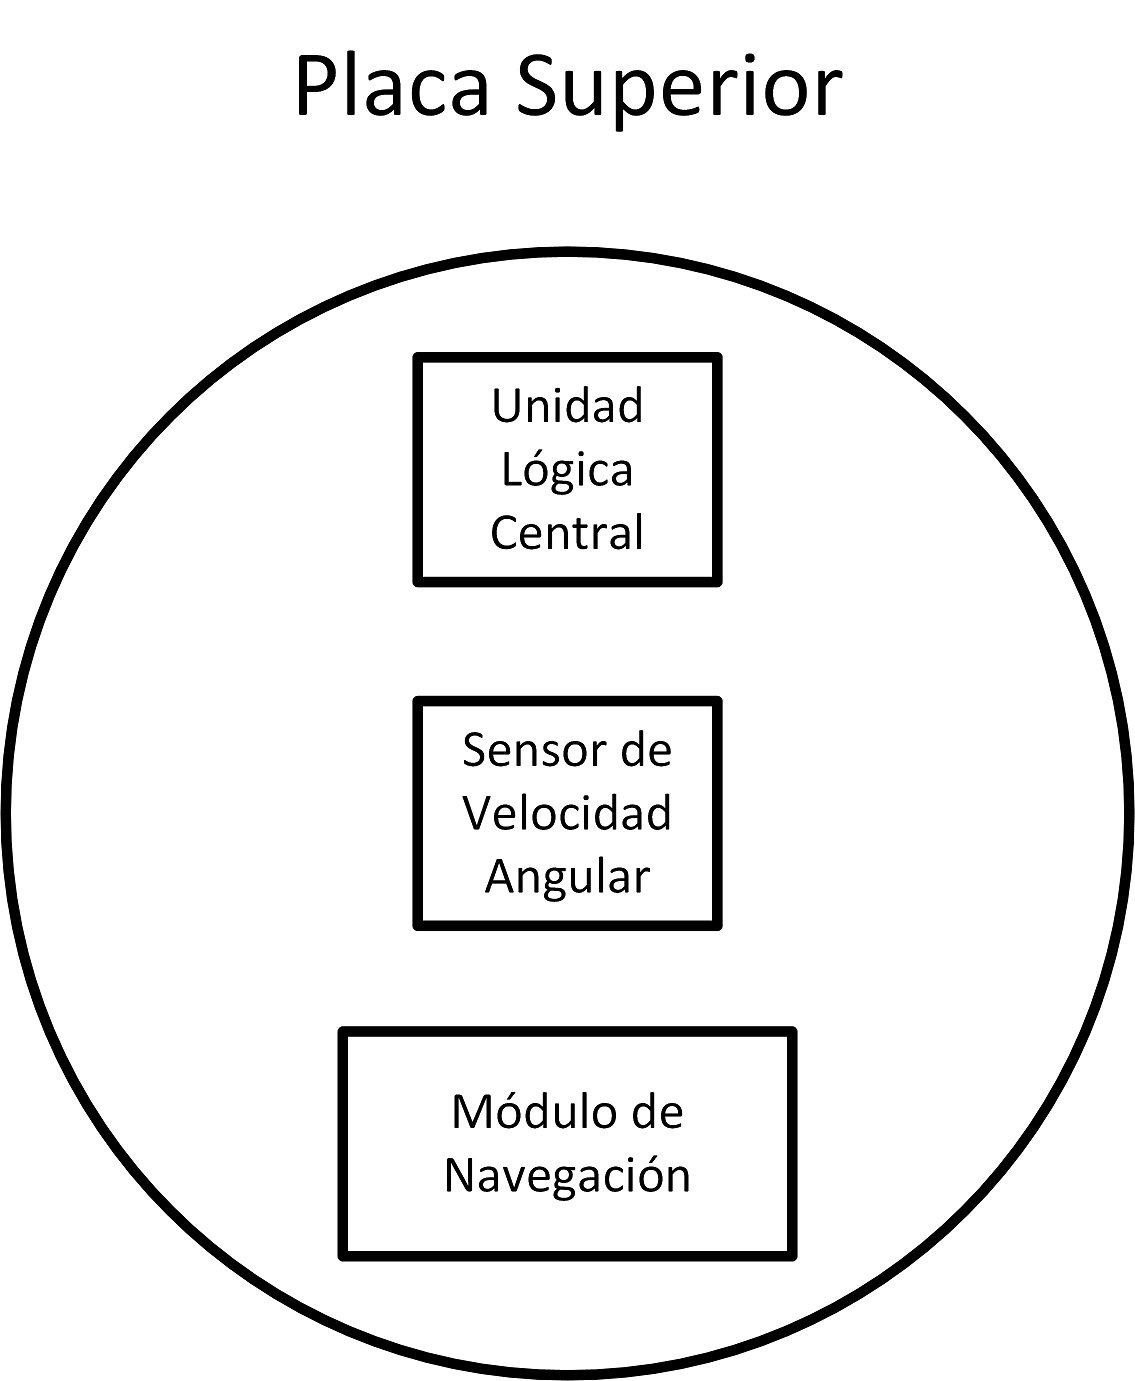
\includegraphics[scale=1.0]{diseniosist/SA/SA1.png}
& 
\includegraphics[scale=1.0]{diseniosist/SA/SA2.png}
&
\includegraphics[scale=1.0]{diseniosist/SA/SA3.png}
\tabularnewline \tabularnewline
  & A1 & A2 & A3
\tabularnewline \midrule
%------------------------------------------------------------------------------------------------
Posici�n (A) ($sS_{1\text{.}2}$)
&
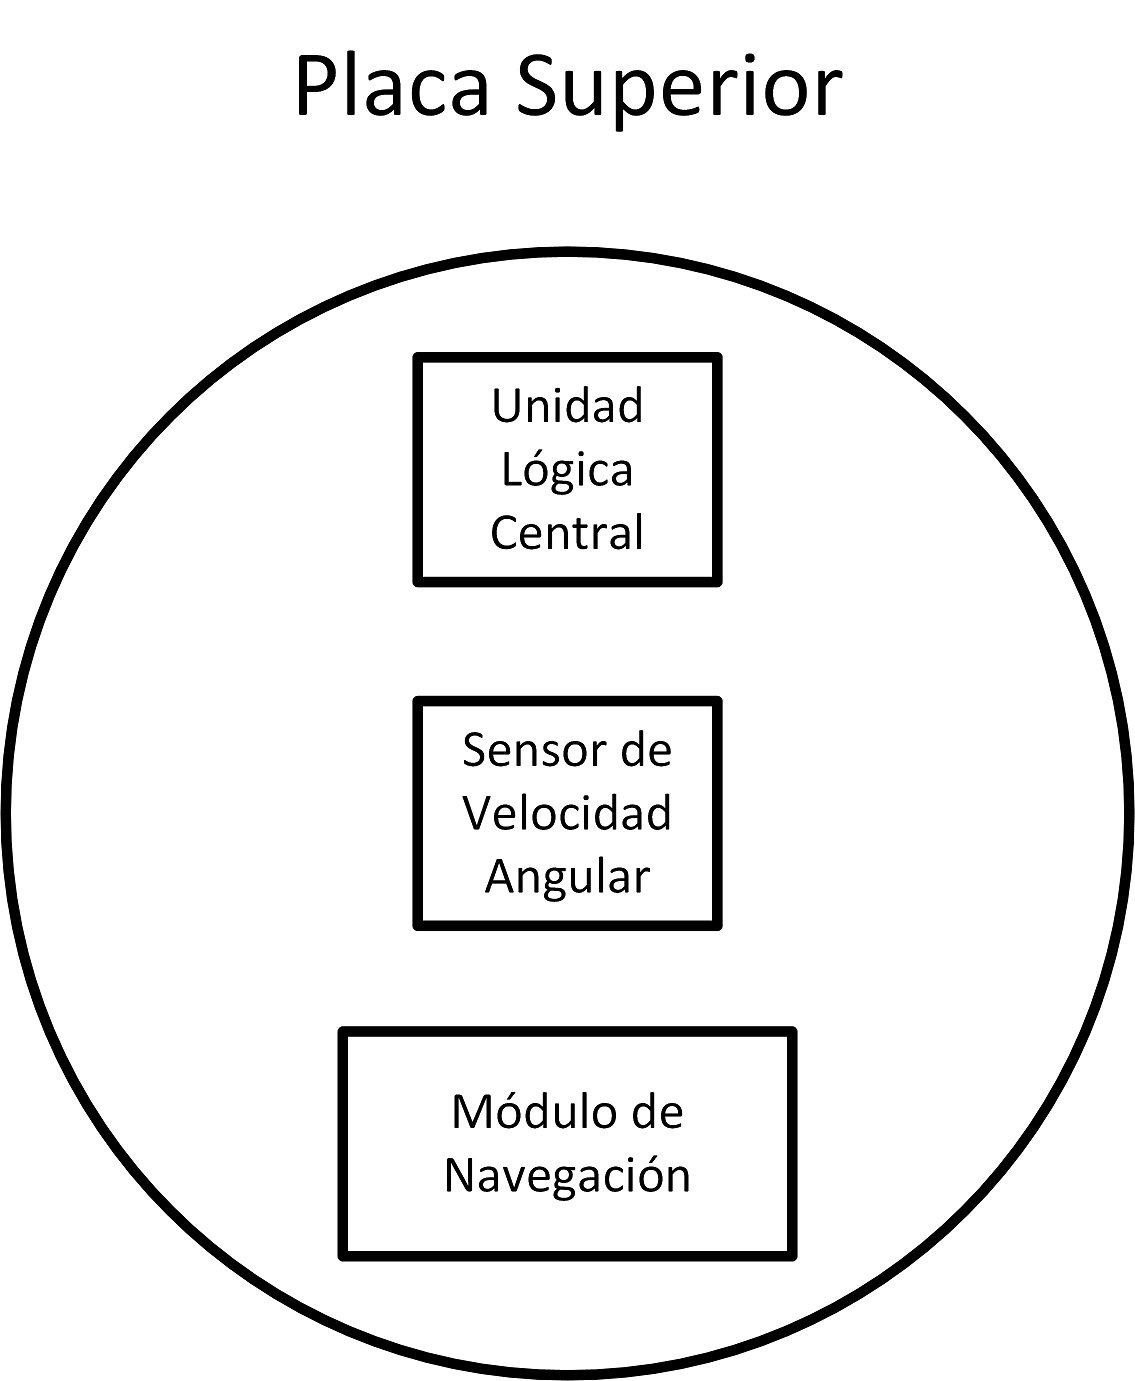
\includegraphics[scale=1.0]{diseniosist/SA/SA1.png}
& 
\includegraphics[scale=1.0]{diseniosist/SA/SA2.png}
&
\includegraphics[scale=1.0]{diseniosist/SA/SA3.png}
\tabularnewline \tabularnewline
  & A1 & A2 & A3
\tabularnewline
%------------------------------------------------------------------------------------------------

\bottomrule
\end{tabular}
}
\end{center}
\end{table}

\begin{table}[H]
\ContinuedFloat
\begin{center}
\caption{An�lisis morfol�gico del CanSat (continuaci�n).}
\resizebox{17cm}{!}{
\begin{tabular}{m{2cm}>{\centering}m{6cm}>{\centering}m{6cm}>{\centering}m{6cm}}
\multicolumn{4}{c}{}\tabularnewline
\toprule
\multicolumn{4}{c}{\textbf{Sistema de Procesamiento de Datos}}\tabularnewline
\midrule
\textbf{Par�metro} & \centering \textbf{Soluci�n 1} & \centering \textbf{Soluci�n 2} & \centering \textbf{Soluci�n 3}\tabularnewline
\hline
\tabularnewline

%------------------------------------------------------------------------------------------------
Posici�n (A) ($sS_{2\text{.}1}$)
&
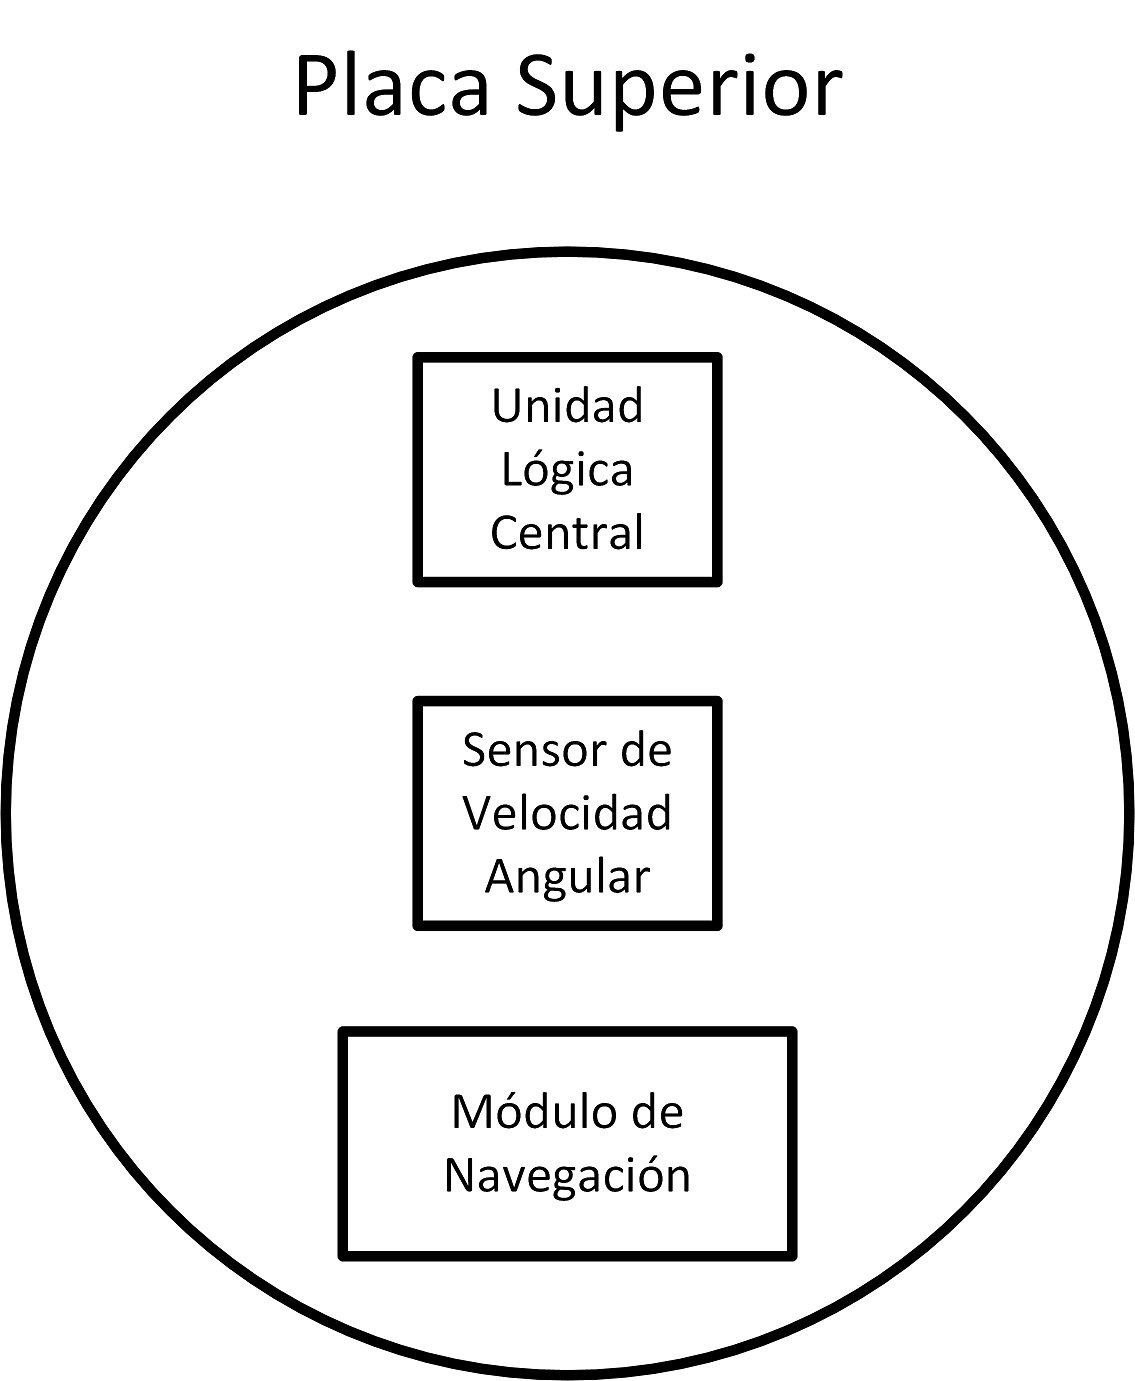
\includegraphics[scale=1.0]{diseniosist/SA/SA1.png}
& 
\includegraphics[scale=1.0]{diseniosist/SA/SA2.png}
&
\includegraphics[scale=1.0]{diseniosist/SA/SA3.png}
\tabularnewline \tabularnewline
  & A1 & A2 & A3
\tabularnewline \midrule
%------------------------------------------------------------------------------------------------
Posici�n (B) ($sS_{2\text{.}2}$)
&
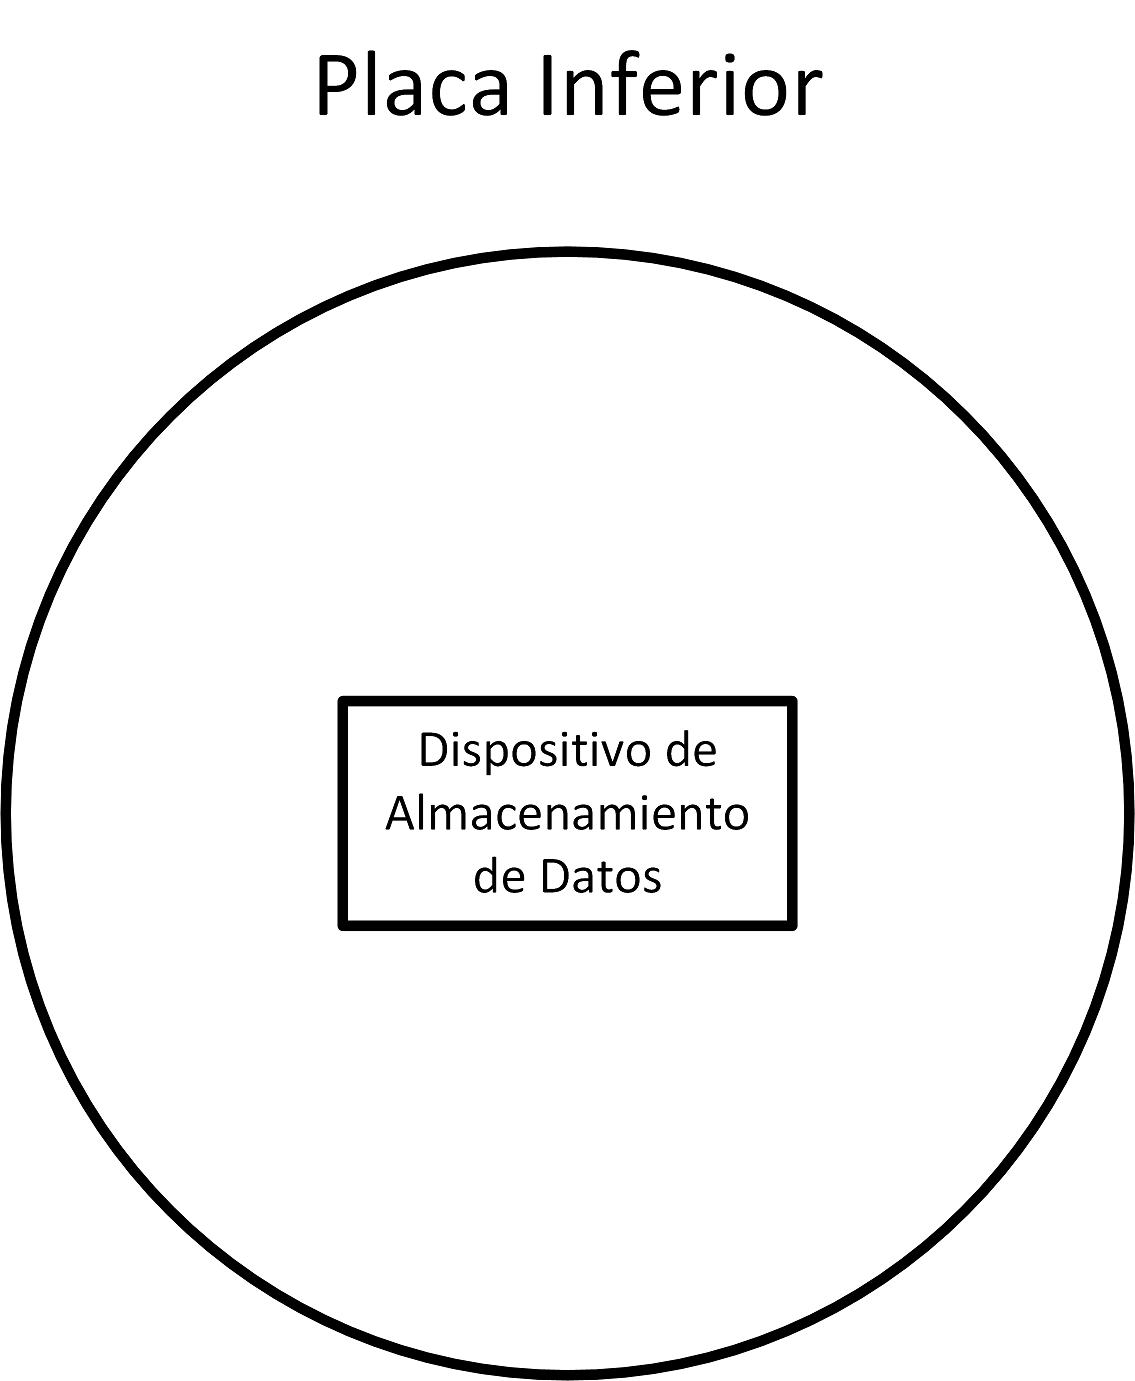
\includegraphics[scale=1.0]{diseniosist/SB/SB1.png}
& 
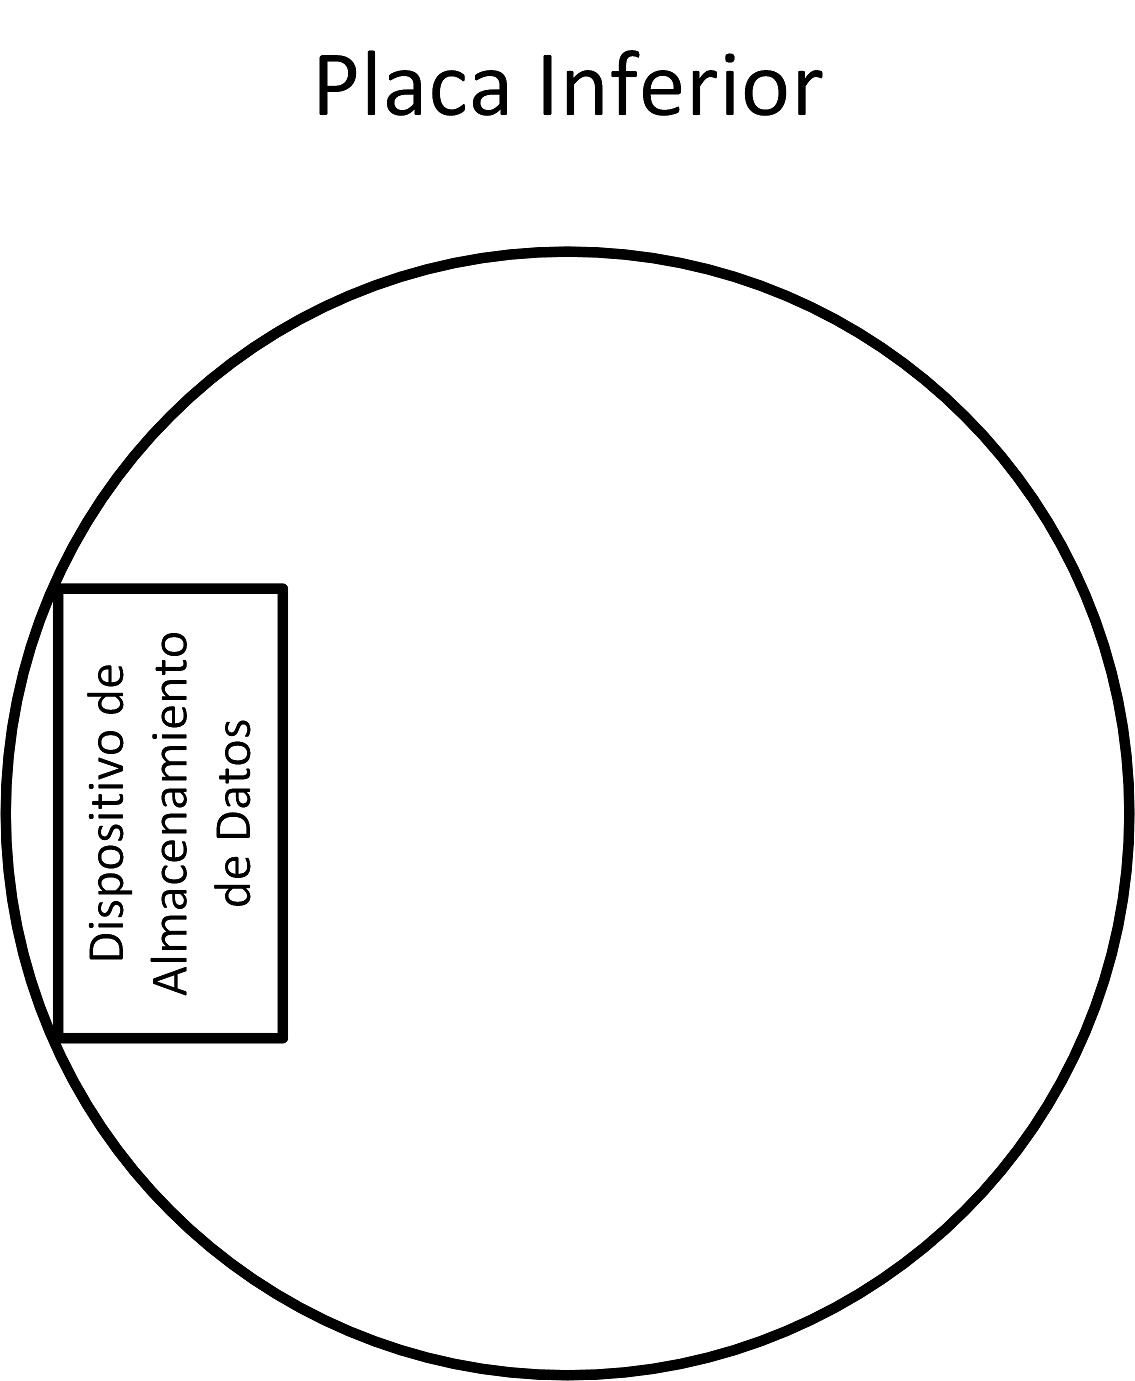
\includegraphics[scale=1.0]{diseniosist/SB/SB2.png}
&
%\includegraphics[scale=0.7]{diseniosist/SA/SA3.png}
\tabularnewline \tabularnewline
  & B1 & B2 & 
\tabularnewline \midrule
%------------------------------------------------------------------------------------------------
M�todo (C) ($sS_{2\text{.}3}$)
&
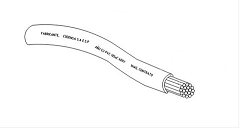
\includegraphics[scale=1.0]{diseniosist/SC/SC1.png}
& 
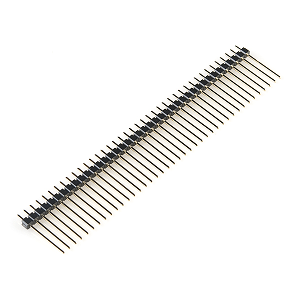
\includegraphics[scale=0.7]{diseniosist/SC/SC2.png}
&
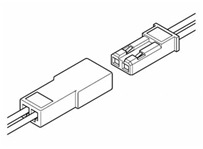
\includegraphics[scale=0.5]{diseniosist/SC/SC3.png}
\tabularnewline
  & C1 & C2 & C3
\tabularnewline
%------------------------------------------------------------------------------------------------

\bottomrule
\end{tabular}
}
\end{center}
\end{table}

\begin{table}[H]
\ContinuedFloat
\begin{center}
\caption{An�lisis morfol�gico del CanSat (continuaci�n).}
\resizebox{17cm}{!}{
\begin{tabular}{m{2cm}>{\centering}m{6cm}>{\centering}m{6cm}>{\centering}m{6cm}}
\multicolumn{4}{c}{}\tabularnewline
\toprule
\multicolumn{4}{c}{\textbf{Sistema de Reducci�n de Velocidad de Descenso}}\tabularnewline
\midrule
\textbf{Par�metro} & \centering \textbf{Soluci�n 1} & \centering \textbf{Soluci�n 2} & \centering \textbf{Soluci�n 3}\tabularnewline
\hline
\tabularnewline

%------------------------------------------------------------------------------------------------
Mecanismo (H) ($sS_{3\text{.}1}$)
&
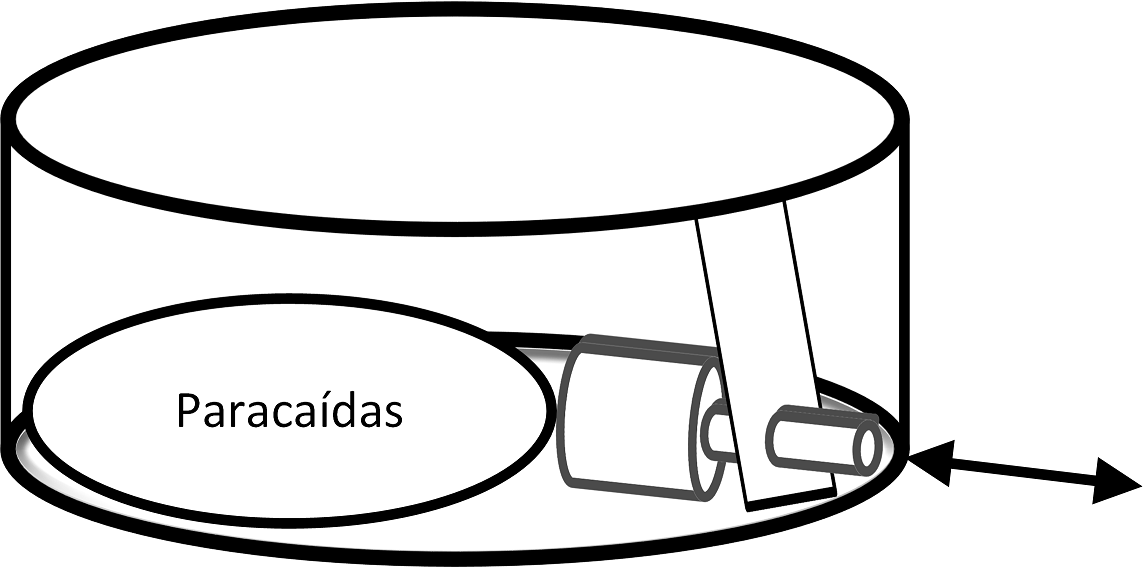
\includegraphics[scale=1.4]{diseniosist/SH/SH1.png}
& 
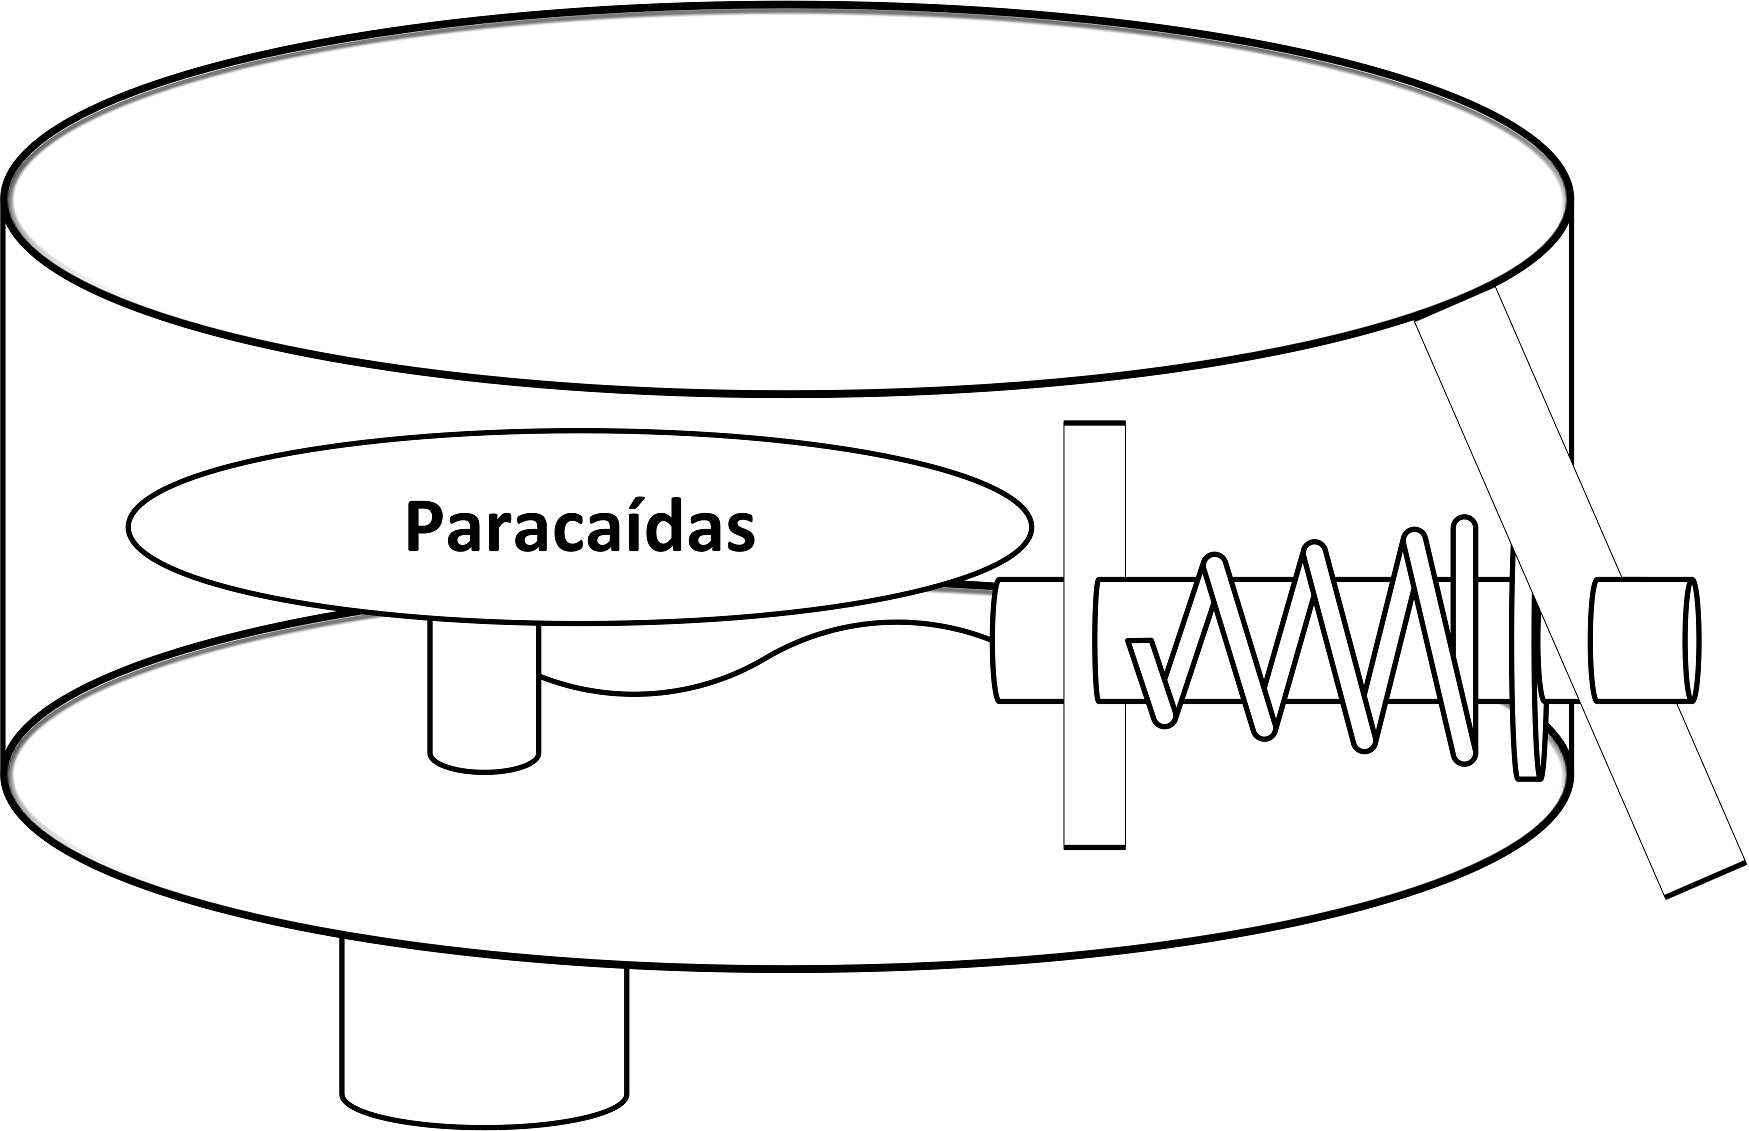
\includegraphics[scale=0.8]{diseniosist/SH/SH2.png}
&
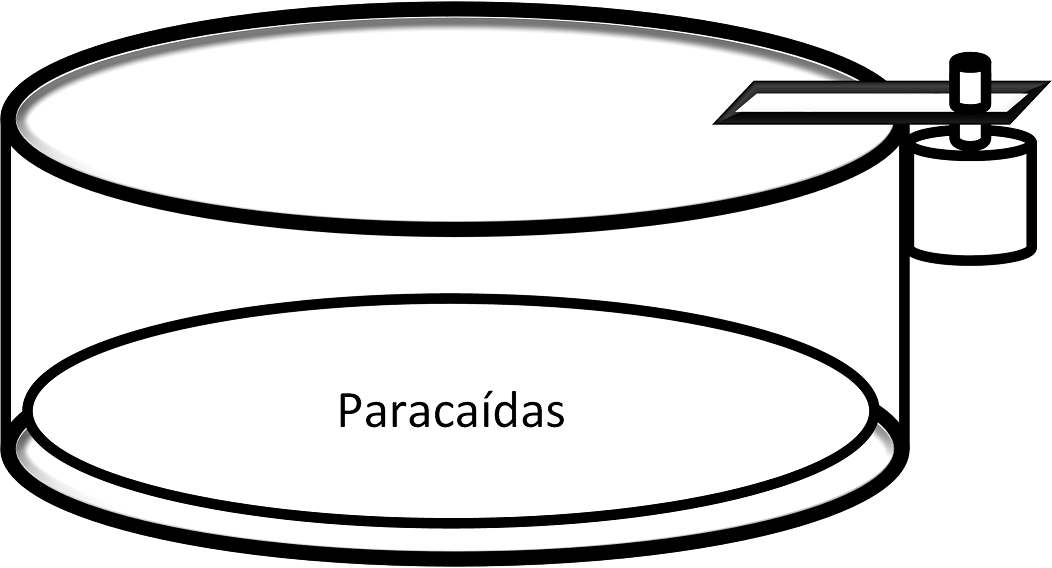
\includegraphics[scale=1.2]{diseniosist/SH/SH3.png}
\tabularnewline
 & H1 & H2 & H3
\tabularnewline
& Atrancamiento con v�stago & Apertura utilizando hilo y resorte & Atrancamiento con tope
\tabularnewline \midrule
%------------------------------------------------------------------------------------------------
Mecanismo (I) ($sS_{3\text{.}2}$)
&
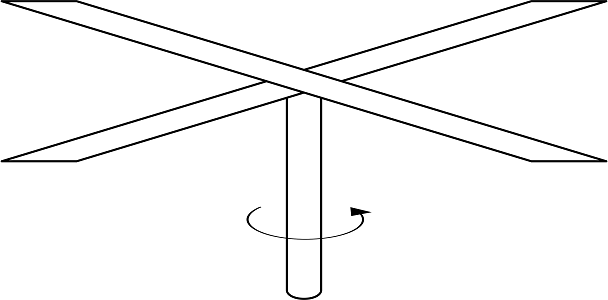
\includegraphics[scale=2.0]{diseniosist/SI/SI1.png}
& 
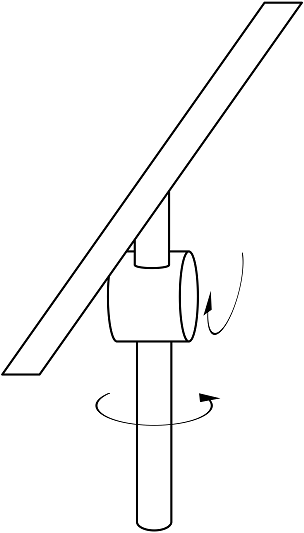
\includegraphics[scale=2.0]{diseniosist/SI/SI2.png}
&
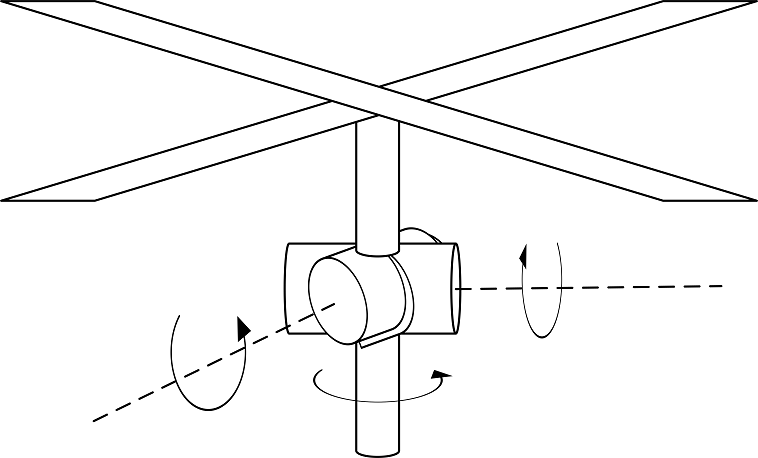
\includegraphics[scale=2.0]{diseniosist/SI/SI3.png}
\tabularnewline
  & I1 & I2 & I3
\tabularnewline
  & 1 GDL & 2 GDL & 3 GDL
\tabularnewline
%------------------------------------------------------------------------------------------------

\bottomrule
\end{tabular}
}
\end{center}
\end{table}


\begin{center}
\resizebox{17cm}{!}{
\begin{tabular}{>{\centering}m{2cm}>{\centering}m{6cm}>{\centering}m{6cm}>{\centering}m{6cm}}
\multicolumn{4}{c}{}\tabularnewline
\toprule
\multicolumn{4}{c}{\textbf{Sistema de Liberaci�n del Veh�culo Cient�fico}}\tabularnewline
\midrule
\textbf{Par�metro} & \centering \textbf{Soluci�n 1} & \centering \textbf{Soluci�n 2} & \centering \textbf{Soluci�n 3}\tabularnewline
\hline
\tabularnewline
  
%------------------------------------------------------------------------------------------------
Mecanismo (L)
&
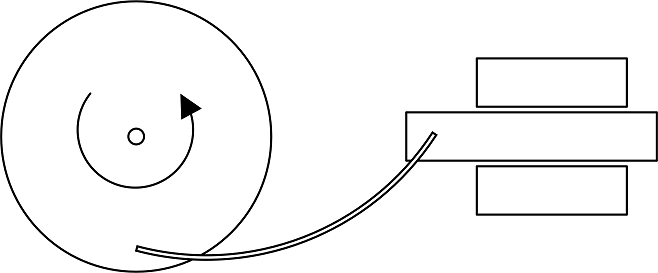
\includegraphics[scale=2.0]{diseniosist/SM/SM1.png}
& 
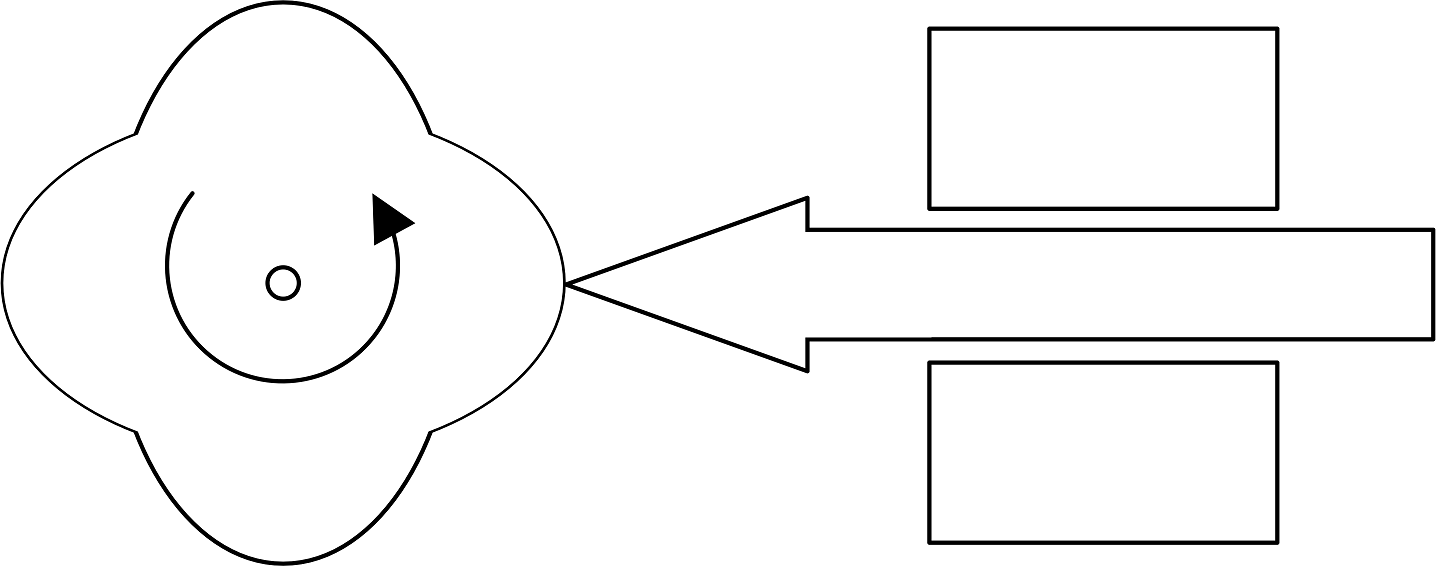
\includegraphics[scale=1.0]{diseniosist/SM/SM2.png}
&
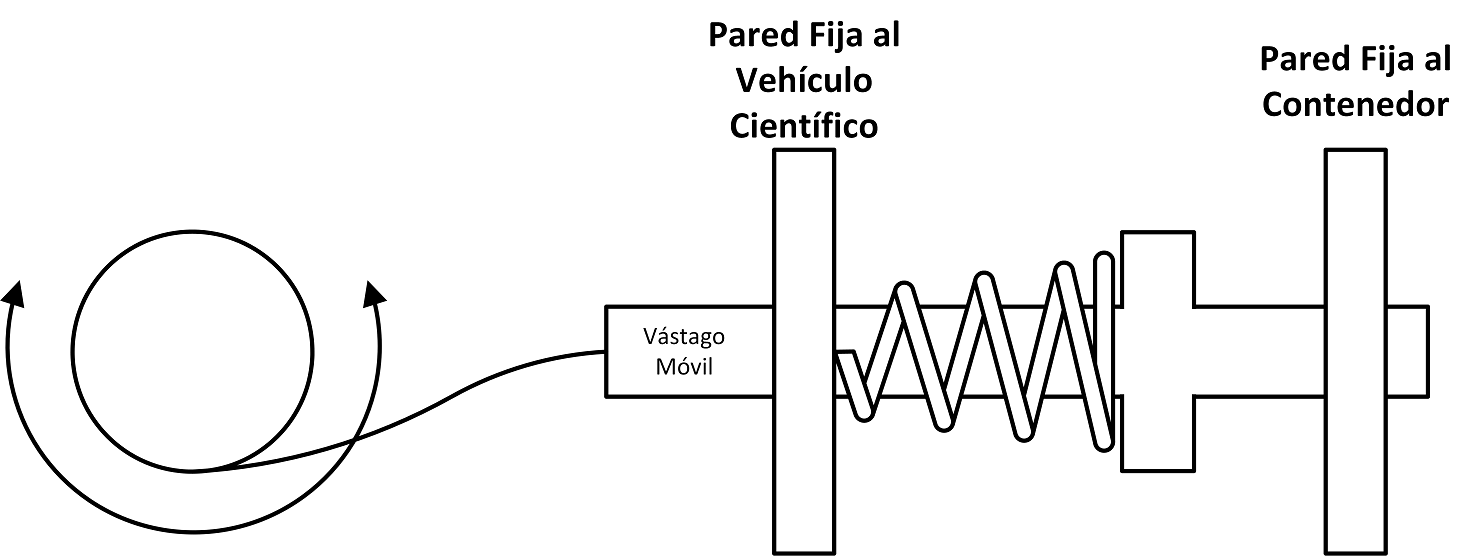
\includegraphics[scale=1.0]{diseniosist/SM/SM3.png}
\tabularnewline
 & L1 & L2 & L3 
\tabularnewline
 & Mecanismo biela$-$manivela$-$corredera & Mecanismo de leva$-$seguidor & Corredera con un hilo
\tabularnewline \midrule
%------------------------------------------------------------------------------------------------
Posici�n (M)
&
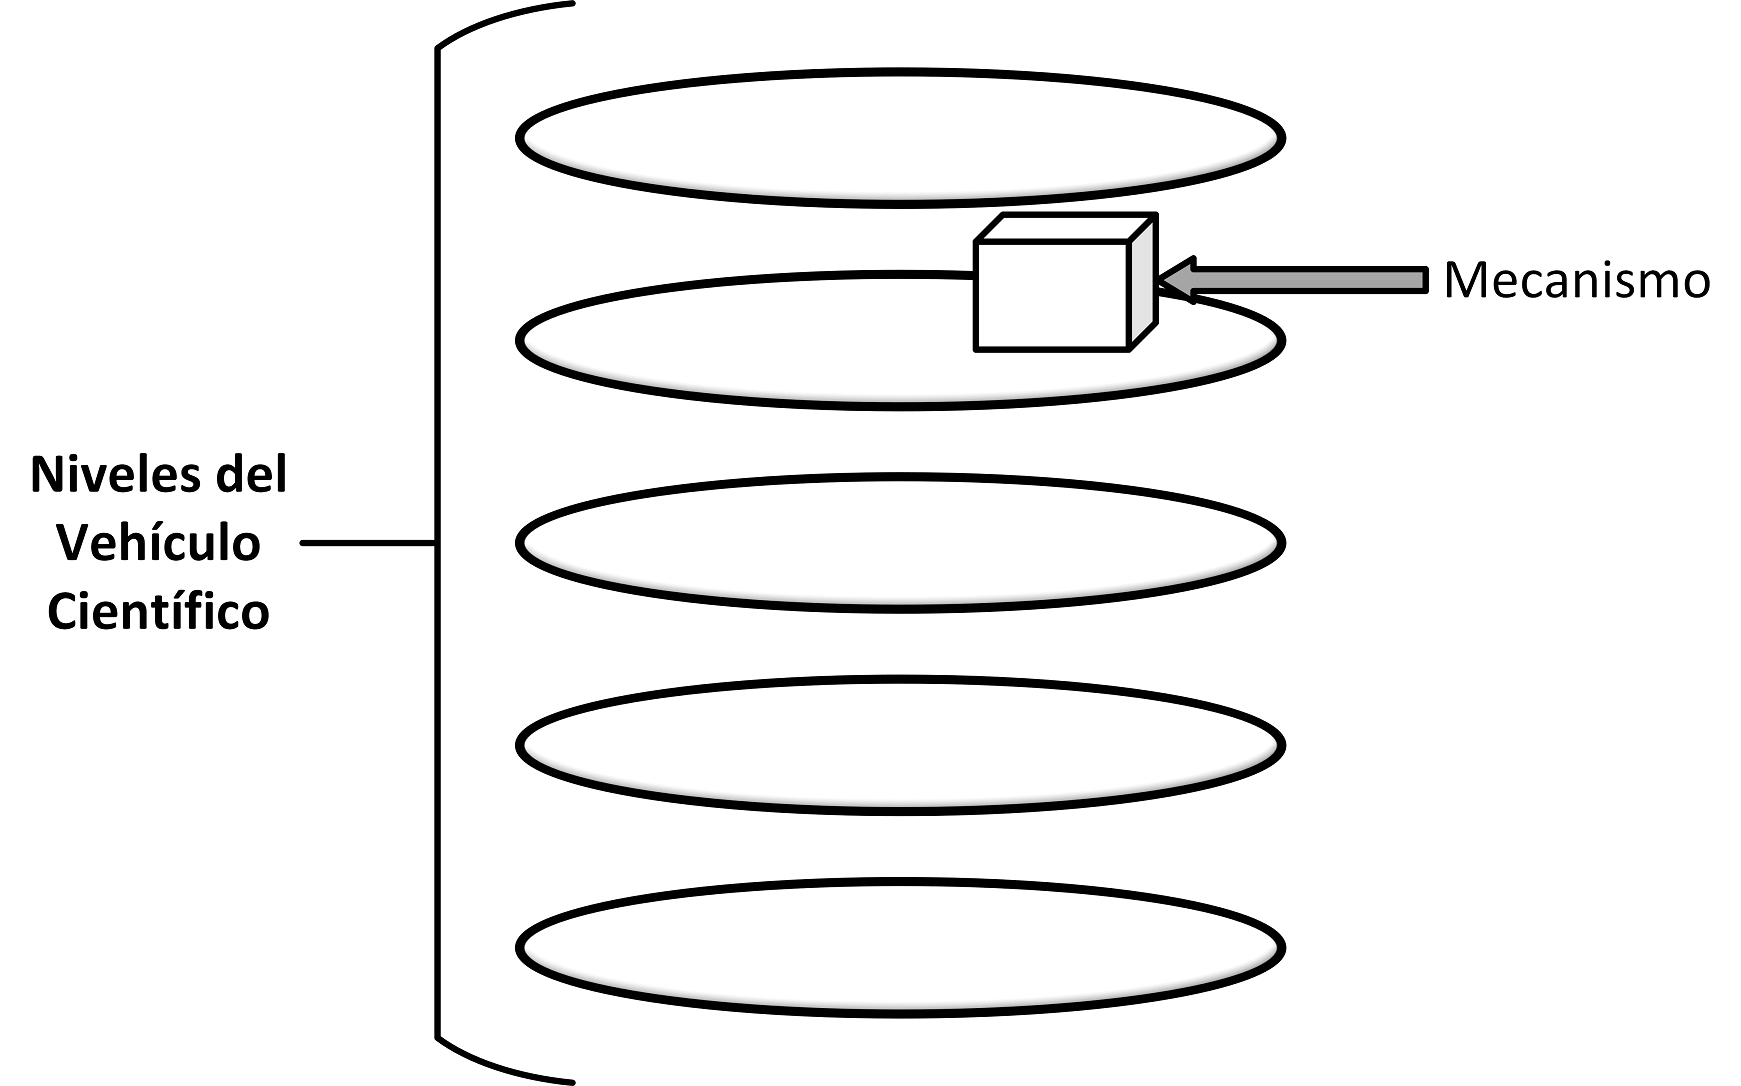
\includegraphics[scale=1.0]{diseniosist/SL/SL1.png}
& 
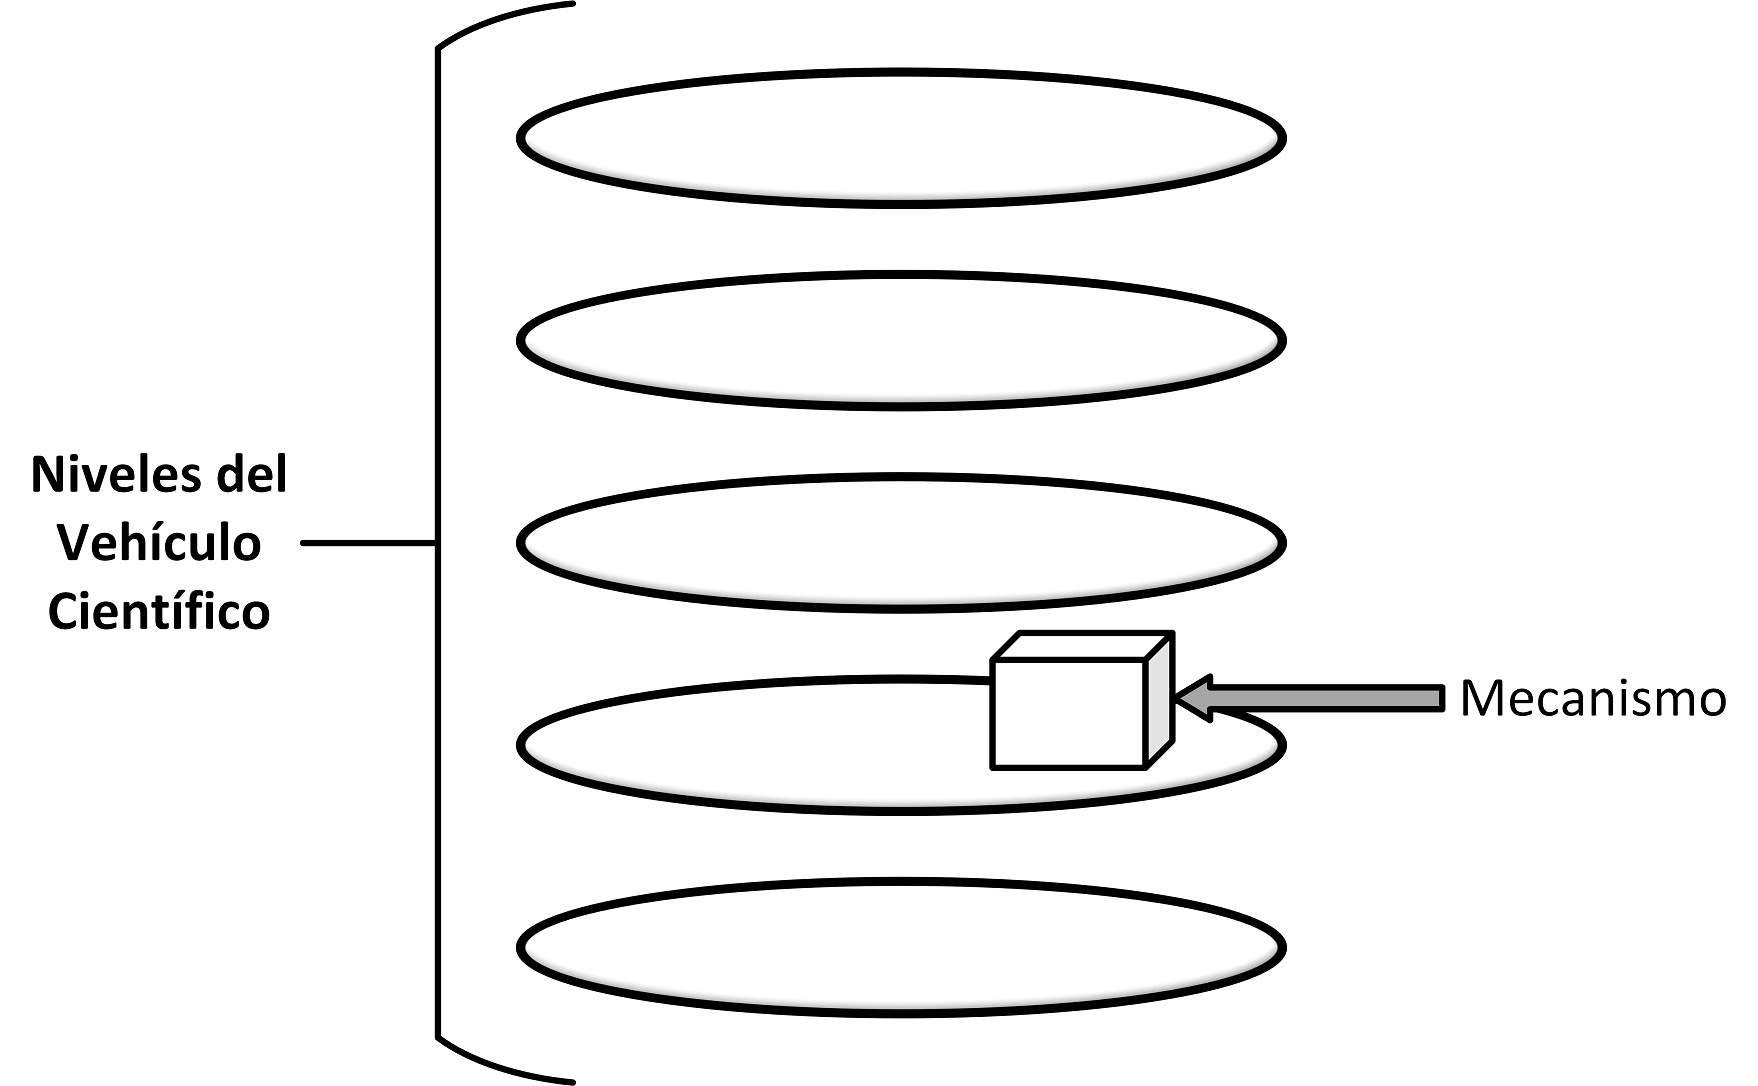
\includegraphics[scale=1.0]{diseniosist/SL/SL2.png}
&
%\includegraphics[scale=0.7]{Imagenes/GMA/SA/SA3.png}
\tabularnewline \tabularnewline
 & M1 & M2 & 
\tabularnewline
%------------------------------------------------------------------------------------------------
\bottomrule
\end{tabular}
}
\end{center}

\newpage

\begin{table}[H]
\ContinuedFloat
\begin{center}
\caption{An�lisis morfol�gico del CanSat (continuaci�n).}
\resizebox{17cm}{!}{
\begin{tabular}{m{2cm}>{\centering}m{6cm}>{\centering}m{6cm}>{\centering}m{6cm}}
\multicolumn{4}{c}{}\tabularnewline
\toprule
\multicolumn{4}{c}{\textbf{Sistema de Registro de Descenso}}\tabularnewline
\midrule
\textbf{Par�metro} & \centering \textbf{Soluci�n 1} & \centering \textbf{Soluci�n 2} & \centering \textbf{Soluci�n 3}\tabularnewline
\hline
\tabularnewline

%------------------------------------------------------------------------------------------------
Configuraci�n (F)
&
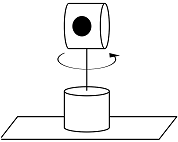
\includegraphics[scale=0.6]{diseniosist/SF/SF1.png}
& 
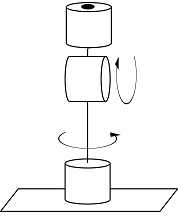
\includegraphics[scale=0.6]{diseniosist/SF/SF2.png}
&
%\includegraphics[scale=0.7]{Imagenes/GMA/SA/SA3.png}
\tabularnewline
 & F1 & F2 & 
 \tabularnewline
 & 1 GDL & 2 GDL & 
\tabularnewline \midrule
%------------------------------------------------------------------------------------------------
Posici�n (G)
&
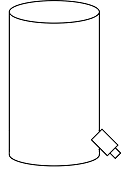
\includegraphics[scale=0.6]{diseniosist/SG/SG1.png}
& 
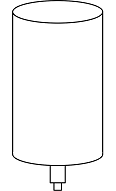
\includegraphics[scale=0.6]{diseniosist/SG/SG2.png}
&
%\includegraphics[scale=0.7]{Imagenes/GMA/SA/SA3.png}
\tabularnewline
 & G1 & G2 & 
 \tabularnewline
 & Sobre la circunferencia, hasta abajo & Al centro, hasta abajo & 
\tabularnewline
%------------------------------------------------------------------------------------------------

\bottomrule
\end{tabular}
}
\end{center}
\end{table}


\begin{center}
\resizebox{17cm}{!}{
\begin{tabular}{m{2cm}>{\centering}m{6cm}>{\centering}m{6cm}>{\centering}m{6cm}}
\multicolumn{4}{c}{}\tabularnewline
\toprule
\multicolumn{4}{c}{\textbf{Sistema de Estaci�n en Tierra}}\tabularnewline
\midrule
\textbf{Par�metro} & \centering \textbf{Soluci�n 1} & \centering \textbf{Soluci�n 2} & \centering \textbf{Soluci�n 3}\tabularnewline
\hline
\tabularnewline

%------------------------------------------------------------------------------------------------
Posici�n (J) ($sS_{6\text{.}1}$)
&
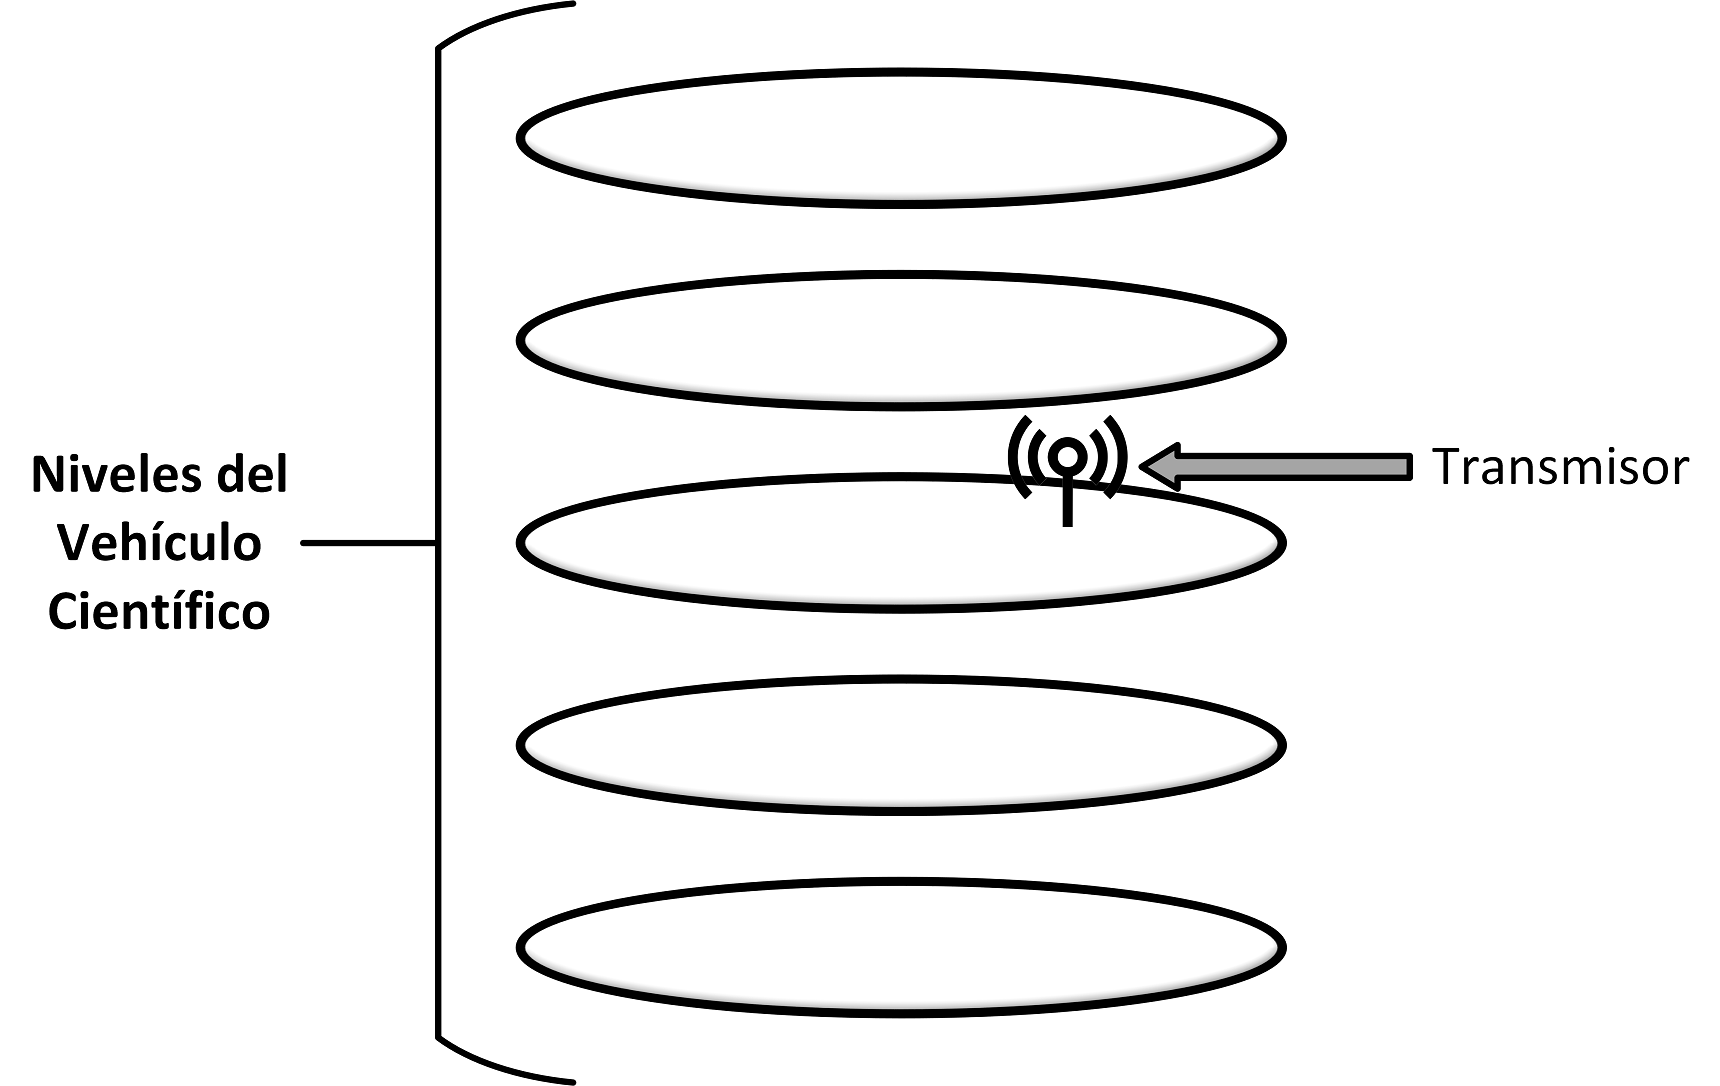
\includegraphics[scale=1.0]{diseniosist/SJ/SJ1.png}
& 
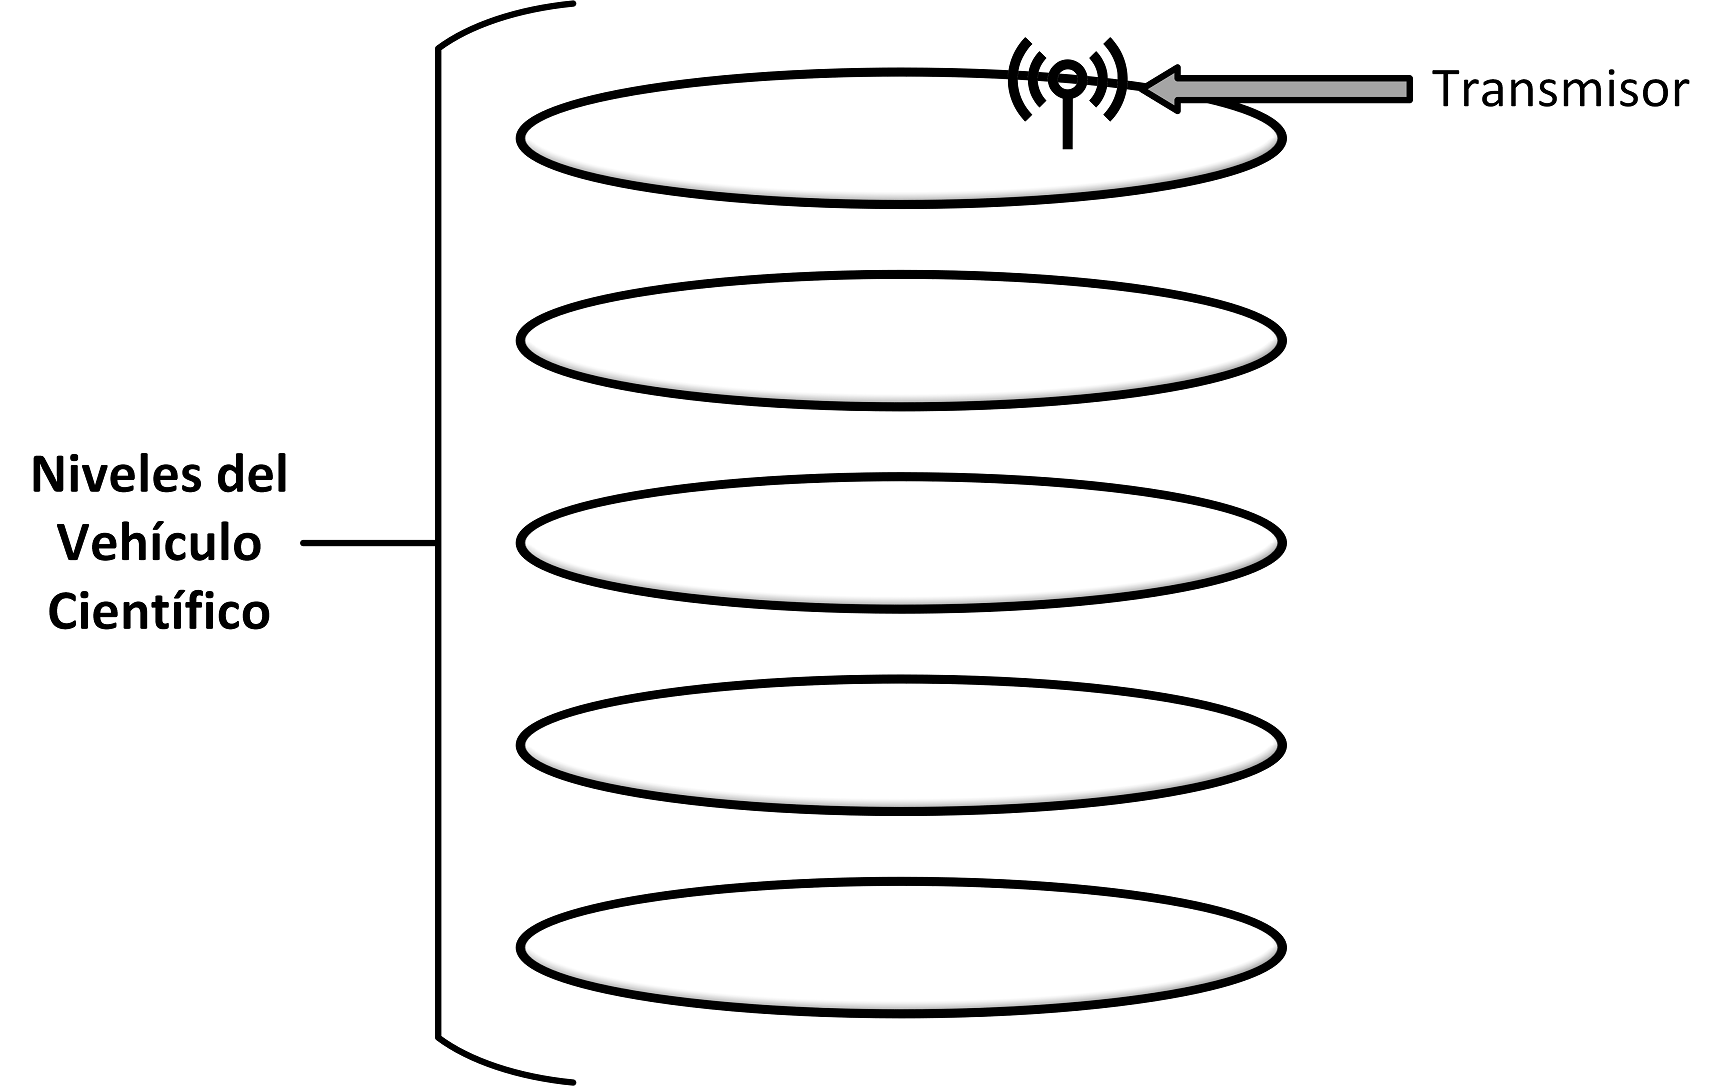
\includegraphics[scale=1.0]{diseniosist/SJ/SJ2.png}
&
%\includegraphics[scale=0.5]{Imagenes/GMA/SJ/SJ3.png}
\tabularnewline
 & J1 & J2 & 
\tabularnewline \midrule
%------------------------------------------------------------------------------------------------
M�todo (K) ($sS_{6\text{.}2}$)
&
IHM 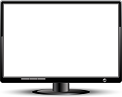
\includegraphics[scale=1.0]{diseniosist/SJ/CP.png}
& 
%\includegraphics[scale=0.7]{Imagenes/GMA/SA/SA2.png}
&
%\includegraphics[scale=0.7]{Imagenes/GMA/SA/SA3.png}
\tabularnewline
 & K1 & & 
\tabularnewline
%------------------------------------------------------------------------------------------------

\bottomrule
\end{tabular}
}
\end{center}

\newpage

\begin{table}[H]
\ContinuedFloat
\begin{center}
\caption{An�lisis morfol�gico del CanSat (continuaci�n).}
\resizebox{17cm}{!}{
\begin{tabular}{m{2cm}>{\centering}m{6cm}>{\centering}m{6cm}>{\centering}m{6cm}}
\multicolumn{4}{c}{}\tabularnewline
\toprule
\multicolumn{4}{c}{\textbf{Sistema de Energ�a}}\tabularnewline
\midrule
\textbf{Par�metro} & \centering \textbf{Soluci�n 1} & \centering \textbf{Soluci�n 2} & \centering \textbf{Soluci�n 3}\tabularnewline
\hline
\tabularnewline

%------------------------------------------------------------------------------------------------
M�todo (C)
&
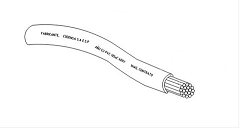
\includegraphics[scale=1.0]{diseniosist/SC/SC1.png}
& 
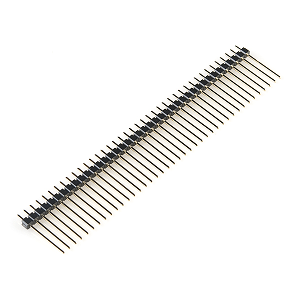
\includegraphics[scale=0.7]{diseniosist/SC/SC2.png}
&
\includegraphics[scale=0.5]{diseniosist/SC/SC3.png}
\tabularnewline
 & C1 & C2 & C3
\tabularnewline \midrule \tabularnewline
%------------------------------------------------------------------------------------------------
Posici�n (D)
&
\includegraphics[scale=1.0]{diseniosist/SD/SD1.png}
& 
\includegraphics[scale=1.0]{diseniosist/SD/SD2.png}
&
%\includegraphics[scale=0.7]{Imagenes/GMA/SA/SA3.png}
\tabularnewline
 & D1 & D2 & 
\tabularnewline
%------------------------------------------------------------------------------------------------

\bottomrule
\end{tabular}
}
\end{center}
\end{table}


\begin{center}
\resizebox{17cm}{!}{
\begin{tabular}{m{2cm}>{\centering}m{6cm}>{\centering}m{6cm}>{\centering}m{6cm}}
\multicolumn{4}{c}{}\tabularnewline
\toprule
\multicolumn{4}{c}{\textbf{Sistema Estructural}}\tabularnewline
\midrule
\textbf{Par�metro} & \centering \textbf{Soluci�n 1} & \centering \textbf{Soluci�n 2} & \centering \textbf{Soluci�n 3}\tabularnewline
\hline
\tabularnewline

%------------------------------------------------------------------------------------------------
Forma (E)
&
\includegraphics[scale=1.0]{diseniosist/SE/SE1.png}
& 
\includegraphics[scale=1.0]{diseniosist/SE/SE2.png}
&
\includegraphics[scale=1.0]{diseniosist/SE/SE3.png}
\tabularnewline
 & E1 & E2 & E3 
\tabularnewline
%------------------------------------------------------------------------------------------------

\bottomrule
\end{tabular}
}
\end{center}

\newpage

		\subsection{Selecci�n del concepto final}			
\noindent A�n cuando se han descartado las combinaciones que presentan inconsistencias entre s�, el n�mero restante de combinaciones puede todav�a ser grande. Debido a lo anterior, s�lo se evaluar�n $3$ combinaciones para obtener s�lo una que corresponder� al dise�o preliminar del CanSat. El dise�o preliminar seleccionado servir� como punto de partida para el dise�o detallado. La Tabla \ref{tab:Combinacion} muestra las combinaciones a ser evaluadas.

\begin{table}[H]
\begin{center}
\caption{Combinaciones de soluciones a evaluar para la selecci�n del die�o preliminar.}
\label{tab:Combinacion}
\resizebox{14cm}{!}{
\begin{tabular}{p{4cm}p{12cm}}
\multicolumn{2}{c}{}\tabularnewline
\toprule

\multicolumn{1}{c}{\textbf{Combinaci�n}} & \multicolumn{1}{c}{\textbf{Elementos}}
\tabularnewline
\hline
\tabularnewline

\centering 1 & \centering A1, B2, C3, D1, E1, F1, G2, H1, I2, J1, K1, L1, M1\tabularnewline
\centering 2 & \centering A3, B2, C1, D1, E3, F1, G2, H3, I1, J1, K1, L2, M2\tabularnewline
\centering 3 & \centering A3, B2, C3, D1, E1, F1, G2, H2, I3, J1, K1, L3, M1\tabularnewline

\bottomrule
\end{tabular}
}
\end{center}
\end{table}

\noindent El m�todo AHP fue utilizado para seleccionar la mejor combinaci�n de soluciones con base en varios criterios. La Tabla \ref{tab:CriteriosCombinacion} muestra estos criterios. Finalmente, la Tabla \ref{tab:priorizacion de combinaciones} muestra el n�mero de prioridad de cada combinaci�n resultado del m�todo AHP.

\begin{table}[H]
\begin{center}
\caption{Criterios para la selecci�n de dise�o preliminar.}
\label{tab:CriteriosCombinacion}
\resizebox{14cm}{!}{
\begin{tabular}{p{4cm}p{6cm}p{5cm}}
\multicolumn{3}{c}{}\tabularnewline
\toprule

\centering \textbf{Criterio} & \centering \textbf{Descripci�n} & \centering \textbf{Escala}\tabularnewline
\hline
\tabularnewline

Estabilidad & Se hace referencia a c�mo es modificado el centro de gravedad del CanSat para mantenerlo alineado con el nadir. & Mientras m�s abajo se encuentre el centro de gravedad, mejor.\tabularnewline\tabularnewline

Fiabilidad de conexiones el�ctricas & Se hace referencia a qu� tan confiables son las terminales de conexi�n el�ctricas. & Entre menos susceptibles sean a desoldarse, desconectarse o romperse, mejor.\tabularnewline\tabularnewline

Control & Se hace referencia a la presencia de grados de libertad a controlar en el SRD. & Entre menor cantidad de grados de libertad, mejor.\tabularnewline\tabularnewline

Fiabilidad de conexiones estructurales & Se hace referencia a la presencia de elementos estructurales flexibles y sensibles a vibraciones. & Entre menos resortes o hilos, mejor.\tabularnewline\tabularnewline

\bottomrule
\end{tabular}
}
\end{center}
\end{table}

\begin{table}[H]
\ContinuedFloat
\begin{center}
\caption{Criterios para la selecci�n de dise�o preliminar (continuaci�n).}
\resizebox{14cm}{!}{
\begin{tabular}{p{4cm}p{6cm}p{5cm}}
\multicolumn{3}{c}{}\tabularnewline
\toprule

\centering \textbf{Criterio} & \centering \textbf{Descripci�n} & \centering \textbf{Escala}\tabularnewline
\hline
\tabularnewline

Modularidad & Se hace referencia a la compatibilidad que tendr� el SP con CanSats futuros. & Entre m�s independiente sea el SP del resto de sistemas y subsistemas, mejor.\tabularnewline\tabularnewline

Cantidad de piezas & Se hace referencia a la cantidad de piezas m�viles.& Entre menos piezas m�viles, mejor.\tabularnewline\tabularnewline

Geometr�a & Se hace referencia a la geometr�a de las piezas. & Entre m�s sencilla sea la geometr�a, mejor.\tabularnewline\tabularnewline

Ensamble & Se hace referencia al ensamble y reemplazo de partes. & Entre m�s sencillo y r�pido sea el ensamble, mejor.\tabularnewline\tabularnewline

Espacio requerido & Se refiere a la cantidad de espacio necesario para albergar los componentes y efectuar los movimientos de los mecanismos. & A menor espacio requerido, mejor.\tabularnewline\tabularnewline

Rigidez & Se hace referencia a la firmeza del ensamble final. & Entre m�s firme, mejor.\tabularnewline\tabularnewline

Visibilidad & Se hace referencia al campo visual efectivo de la c�mara. & Entre mayor sea el campo visual, mejor.\tabularnewline\tabularnewline

Distribuci�n componentes & Se hace referencia a la densidad de componentes por placa de circuito. & Entre mayor cantidad de componentes est�n en una sola placa, mejor.\tabularnewline\tabularnewline

Extracci�n & Se hace referencia a la extracci�n del componente de almacenamiento y las bater�as del CanSat. & Entre m�s r�pida y sencilla sea la extracci�n, mejor.

\tabularnewline

\bottomrule
\end{tabular}
}
\end{center}
\end{table}


\begin{table}[H]
\begin{center}
\caption{Resultados del proceso de priorizaci�n de combinaciones para el dise�o preliminar.}
\label{tab:priorizacion de combinaciones}
\resizebox{13cm}{!}{
\begin{tabular}{p{8cm}p{3cm}p{3cm}}
\multicolumn{3}{c}{}\tabularnewline
\toprule

\textbf{Combinaci�n} & \textbf{Posici�n} & \textbf{Valor}
\tabularnewline
\hline
\tabularnewline
  
\rowcolor{lightgray}Combinaci�n 1 & \textbf{1} & 0.4418\tabularnewline
Combinaci�n 2 & 3 & 0.2514\tabularnewline
Combinaci�n 3 & 2 & 0.3069\tabularnewline

\bottomrule
\end{tabular}
}
\end{center}
\end{table}

\noindent La imagen \ref{img:ConceptoFinal} muestra un bosquejo del dise�o preliminar del CanSat.

% El m�dulo de sensores estar� sobrepuesto en la misma placa que el resto de la circuiter�a, lo que le da al SP la cualidad de modular. El dispositivo de almacenamiento de datos estar� colocado en el per�metro de la placa de circuito para su f�cil extracci�n. Las conexiones el�ctricas utilizar�n cables con conectores r�gidos en los extremos para evitar desconexiones. Se utilizar� un mecanismo de atrancamiento con v�stago para la apertura del paraca�das del SRV-P. Para el mecanismo del SRV-A se utilizar� un sistema de rotor semir�gido con 2 GDL. El transmisor del SC-ET  estar� colocado en el centro del CanSat. Para el SU-ET se desarrollar� una interfaz de usuario para mostrar los datos enviados por el CanSat, y almacenarlo en Tierra. El SLVC utilizar� un mecanismo de biela-manivela-corredera y se ubicar� en la parte de arriba del CanSat, justo debajo del SRV-A. El mecanismo del SRD tendr� 1 GDL: movimiento de azimuth, y estar� ubicado hasta la parte m�s baja del CanSat para que la c�mara tenga buena visibilidad. La bater�a estar� colocada al centro del CanSat, y la estructura de �ste ser� cil�ndrica.\\


\begin{figure}[H]
	\centering
		\includegraphics[angle = -90, scale=0.50]{diseniosist/ConceptoFinalCanSat}
	\caption{Dise�o preliminar del CanSat.}
	\label{img:ConceptoFinal}
\end{figure}


% ******************************************************************************************************************************%	
	\section{Dise�o detallado}
		% !TeX encoding = ISO-8859-1
El Cansat est� constituido de dos elementos: el contenedor, que tiene la finalidad de envolver parcialmente al veh�culo cient�fico, as� como encerrar el parac�das; y el veh�culo cient�fico, el cual realiza las tareas pricipales de la misi�n como obtener, procesar y enviar las variables f�sicas del entorno.\\

\noindent Como se muestra en la figura \ref{img:DisenosCansat} se realizaron tres dise�os del veh�culo cient�fico y del contenedor. La principal raz�n del cambio de geometr�a fue la masa resultante. La masa del Cansat asociado al primer dise�o era de 570 [g], en el segundo dise�o la masa se redujo a 530 [g] y, finalemnte, en el tercer dise�o la masa lleg� a ser de 510 [g].

\begin{figure}[H]
	\centering
	\includegraphics[scale=0.60]{imgmeca/DisenosCansat.png}
	\caption{Dise�os realizados del Cansat siendo el �ltimo (de izquierda a derecha) el seleccionado para construir.}
	\label{img:DisenosCansat}
\end{figure}

\noindent La figura \ref{img:DisenosCansat} es una muestra de que el proceso de dise�o en ingenier�a es inevitablemente iterativo, en d�nde cada iteraci�n representa un mejor entendimiento de los requerimientos y las restricciones del sistema. Dicho entendimiento se refleja en las modificaciones hechas al dise�o en cada iteraci�n.

\newpage
		\subsection{Sistema Central de Manejo del Comportamiento} \label{sistSCMC}
% !TeX encoding = ISO-8859-1

%%%%%%%%%%%%%%%%%%%%%%%%%%%%%%%%%%%%%%%%%%%%%%%%%%%%%%%%%%%%%%%%%%%%%%%%%%%%%%%%%%%%%%%%%%%%%%%%%%%%%%%%%%%
%%%%%%%%%%%%%%%%%%%%%%%%%%%%%%%%%%%%%%%%%%%%%%%%%%%%%%%%%%%%%%%%%%%%%%%%%%%%%%%%%%%%%%%%%%%%%%%%%%%%%%%%%%%
%%%%%%%%%%%%%%%%%%%%%%%%%%%%%%%%%%%%%%%%%%%%%%%%%%%%%%%%%%%%%%%%%%%%%%%%%%%%%%%%%%%%%%%%%%%%%%%%%%%%%%%%%%%


\algblockdefx[SwitchCase]{Switch}{EndSwitch}%
	[1]{\textbf{switch} ( #1 )}%
	{}
	
\algblockdefx[Case]{Case}{Break}%
	[1]{\textbf{case} \textit{#1}:}%
	{\textbf{break}}
	
	
%%%%%%%%%%%%%%%%%%%%%%%%%%%%%%%%%%%%%%%%%%%%%%%%%%%%%%%%%%%%%%%%%%%%%%%%%%%%%%%%%%%%%%%%%%%%%%%%%%%%%%%%%%%
%%%%%%%%%%%%%%%%%%%%%%%%%%%%%%%%%%%%%%%%%%%%%%%%%%%%%%%%%%%%%%%%%%%%%%%%%%%%%%%%%%%%%%%%%%%%%%%%%%%%%%%%%%%
%%%%%%%%%%%%%%%%%%%%%%%%%%%%%%%%%%%%%%%%%%%%%%%%%%%%%%%%%%%%%%%%%%%%%%%%%%%%%%%%%%%%%%%%%%%%%%%%%%%%%%%%%%%	
	
	
	
{\parindent0pt

\indent El SCMC realiza las funciones de adquirir todas las variables internas y externas del CanSat y las env�a al SPD. El SPD entonces procesa dichas variables crudas y las env�a de regreso al SCMC para que �ste tome decisiones de acuerdo a los requerimientos de la misi�n.\\

El SCMC est� estrechamente relacionado con el SPD; ambos comparten componentes f�sicos y recursos de procesamiento. Debido al enfoque funcional, el SCMC y el SPD ser�n abordados de manera independiente; primero se hablar� de las funciones y caracter�sticas de ambos sistemas y despu�s de su construcci�n f�sica.\\

El SCMC se compone de $2$ subistemas: el subsistema de percepci�n ($sS_{1{.}1}-$SP)  y el subsistema de toma de decisiones ($sS_{1{.}2}-$STD).\\

\subsubsection{Subsistema de Percepci�n}

El SP realiza la funci�n $f_{2{.}2}-$\textit{Medir par�metros} y todas las subfunciones respectivas (a excepci�n de que se indique lo contrario). Esta informaci�n se utiliza para la toma de decisiones o para el an�lisis posterior en Tierra.\\

Este sistema est� constituido por todos los sensores del CanSat. Para la selecci�n de los sensores se utilizaron matrices de decisi�n en las que se exponen las caracter�sticas m�s cr�ticas de �stos que fueron tomadas en cuenta para la selecci�n. Estas matrices se muestran al final de la descripci�n del SPD.\\

De acuerdo con la Tabla \ref{tab:Funciones}, la funci�n $2.2$ y todas sus subfunciones, exceptuando la subfunci�n $2.2.1.4$, corresponden al SP de tal modo que a continuaci�n se exponen los sensores seleccionados para realizar dichas funciones.\\

\begin{itemize}
	\item \textbf{GPS:} Usado para adquirir datos de hora UTC, latitud, longitud y altitud sobre el nivel del mar. Este elemento atiende a las funciones $2.2.1.1$ y $2.2.2.6$.
	\item \textbf{Bar�metro:} Usado para medir la presi�n atmosf�rica y de �sta obtener la altura relativa. Este elemento atiende a las funciones $2.2.2.2$ y $2.2.2.6$.
	\item \textbf{Term�metro}: Usado para medir la temperatura del ambiente. Este elemento atiende a la funci�n $2.2.2.1$
	\item \textbf{Giroscopio:} Usado para medir la velocidad angular del CanSat en los tres ejes de un sistema cartesiano. Este elemento atiende a la funci�n $2.2.2.4$.
	\item \textbf{Aceler�metro:} Usado para medir las aceleraciones del CanSat en los tres ejes de un sistema cartesiano. Este elemento atiende a la funci�n $2.2.2.3$.
	\item \textbf{Magnet�metro:} Usado para medir las componentes del campo magn�tico de la Tierra a las que est� sometido el CanSat. Este elemento atiende a la funci�n $2.2.2.5$.
	\item \textbf{Encoder incremental:} Usado para medir la velocidad angular del rotor. Este elemento atiende a la funci�n $2.2.1.3$.
\end{itemize}


\subsubsection{Subsistema de Toma de Decisiones}

El STD se encarga de conferirle al CanSat el comportamiento deseado con base en las variables adquiridas por el SP y procesadas por el SPD.\\

El dise�o de este subsistema fue regido por los eventos de la misi�n, as� como aquellos requeridos por el equipo con el fin de realizar pruebas. Este sistema atiende a las funciones $2.1.4-$\textit{Realizar conteo del n�mero de paquetes enviados} y $2.3-$\textit{Tomar decisiones} con todas sus subfunciones.\\

El comportamiento del CanSat es regido por una m�quina de estados. La m�quina de estados se muestra en la figura \ref{img:StateMachine}\\

\begin{figure}[H]
	\centering
		\includegraphics[scale=0.60]{diseniosist/SCMC/StateMachVC}
	\caption{M�quina de estados del veh�culo cient�fico.}
	\label{img:StateMachine}
\end{figure}

La Tabla \ref{EstadosMaquinaVehiculo} describe los estados y la Tabla \ref{TransicionMaquinaVehiculo} describe las condiciones de transici�n entre estados.

\begin{table}[H]
\begin{center}
\caption{Estados de la m�quina de estados del veh�culo cient�fico.}
\label{EstadosMaquinaVehiculo}
\resizebox{14cm}{!}{
\begin{tabular}{p{5cm} p{13cm}}
\multicolumn{2}{c}{}\tabularnewline
\toprule
\multicolumn{1}{c}{\textbf{Evento}} & \multicolumn{1}{c}{\textbf{Descripci�n}}\tabularnewline
\midrule
\tabularnewline

($\text{A}_{\text{VC}}$) Inicio & En este estado se inicializan todos los perif�ricos y sensores del veh�culo cient�fico.\tabularnewline
($\text{B}_{\text{VC}}$) Recuperaci�n del estado anterior & En este estado se lee la memoria no vol�til del veh�culo cient�fico que almacena el �ltimo estado en el que se encontraba el sistema antes de ser reiniciado o encendido. \tabularnewline
($\text{C}_{\text{VC}}$) Diagn�stico del sistema & En este estado se realiza el diagn�stico del sistema, verificando que todos los sensores y perif�ricos respondan como es debido. \tabularnewline
($\text{D}_{\text{VC}}$) Espera de despegue & En este estado el sistema s�lo se encuentra esperando el despegue, no realiza ninguna otra acci�n. En este punto el CanSat debe estar dentro del veh�culo de ascenso.\tabularnewline
($\text{E}_{\text{VC}}$) Ascenso & En este estado el CanSat s�lo realiza lectura, c�mputo y transmisi�n de variables.\tabularnewline
($\text{F}_{\text{VC}}$) Descenso con parac�das & Dentro de este estado el CanSat se encuentra descendiendo con el paraca�das como reductor de velocidad. Se realiza lectura, c�mputo, control y transmisi�n de variables.\tabularnewline
($\text{G}_{\text{VC}}$) Descenso con h�lices & En este estado el veh�culo cient�fico desciende con el sistema de autorrotaci�n. El sistema realiza lectura, c�mputo, control y transmisi�n de variables.\tabularnewline
($\text{H}_{\text{VC}}$) Aterrizaje & En este estado el CanSat se encuentra de nuevo en Tierra. El sistema s�lo activa su dispositivo de localizaci�n.\tabularnewline
\bottomrule
\end{tabular}
}
\end{center}
\vspace{-2.2em}
\end{table}

\begin{table}[H]
\begin{center}
\caption{Condiciones de transici�n de la m�quina de estados del veh�culo cient�fico.}
\label{TransicionMaquinaVehiculo}
\resizebox{14cm}{!}{
\begin{tabular}{ p{3cm} p{13cm} }
\multicolumn{2}{c}{}\tabularnewline
\toprule

\multicolumn{1}{c}{\textbf{Transici�n}} & \multicolumn{1}{c}{\textbf{Descripci�n}}\tabularnewline
\midrule
\tabularnewline

	\centering$\text{1}_{\text{VC}}$ & Todos los sensores se encuentran configurados y operando correctamente.
\tabularnewline
	\centering$\text{2}_{\text{VC}}$ &  En este punto el cambio de estado se realiza de acuerdo con la lectura de la memoria no vol�til del CanSat. El �ltimo estado en el que se haya encontrado el sistema ser� el que se restaurar�. 
\tabularnewline
	\centering$\text{3}_{\text{VC}}$ & El sistema no cambia el estado hasta haber hecho un diagn�stico de los sensores sin reporte de errores. \tabularnewline
	\centering$\text{4}_{\text{VC}}$ & El sistema cambia el estado hasta que se detecte un cambio positivo en la altura de referencia. El cambio debe superar los $10 [m]$ por encima de la altura de referencia.
\tabularnewline
	\centering$\text{5}_{\text{VC}}$ & El sistema cambia el estado hasta que se detecte un cambio negativo en la altura m�xima. El cambio debe superar los $10 [m]$ por debajo de la altura m�xima.
\tabularnewline
	\centering$\text{6}_{\text{VC}}$ & El veh�culo cient�fico cambia el estado hasta encontrarse a una altura de $250 [m]$ por encima de la referencia con una tolerancia de $\pm 10 [m]$.
\tabularnewline
	\centering$\text{7}_{\text{VC}}$ & El estado cambia hasta que el sistema se encuentre de nuevo en la altura de referencia.
\tabularnewline
	\centering$\text{8}_{\text{VC}}$ & El estado cambia hasta que se le env�e un comando de reinicio de estados.
\tabularnewline

\bottomrule
\end{tabular}
}
\end{center}
\end{table}

El Algoritmo \ref{PseudocodigoCanSatP1} corresponde a la m�quina de estados del CanSat. Este algoritmo explica el flujo de actividades dentro del programa del microcontrolador correspondiente al STD.


\begin{algorithm}[H]
\caption{Pseudoc�digo CanSat}
\label{PseudocodigoCanSatP1}
\begin{algorithmic}[1]

\Function{Lectura de sensores}{}
	\State Lee GPS, lee giroscopio, lee aceler�metro, lee magnet�metro, lee presi�n atmosf�rica, lee temperatura, calcula altura actual, calcula marco de referencia actual y realiza control de orientaci�n de la c�mara.
\EndFunction\\

\Function{Transmisi�n y Almacenamiento}{datos de sensores}
	\State Genera la trama de datos
	\State Transmite la trama de datos a estaci�n en Tierra
	\State Guarda la trama de datos en la memoria SD
	\State Guarda el n�mero de trama en la memoria no v�latil
	\State $Conteo Paquetes \gets Conteo Paquetes + 1$
\EndFunction\\

\Procedure{M�quina de vuelo}{}
	\State Configura sensores
	\State Lee memoria no v�latil: estado y n�mero de tramas transmitidas.
	\State Restaura funcionalidades.
	\State $Conteo Actual \gets Conteo Almacenado$
	\State $Estado Actual \gets Estado Almacenado$

	\While{el CanSat est� encendido}
		\Switch{EstadoActual}
		
			 \Case{Diagn�stico del sistema}
			 	\If{ comando de inicio fue recibido }
 				 	\State Prueba comunicaci�n con el GPS
				 	\State Prueba comunicaci�n con la IMU
				 	\State Prueba comunicaci�n con el bar�metro y term�metro
				 	\If{ no errores }
				 		\State Activa secuencia sonora aprobatoria
				 		\State Transmite una se�al aprobatoria en las telecomunicaciones
			 			\State $EstadoActual \gets Espera\enspace del\enspace despegue$
				 	\Else
				 		\State Activa secuencia sonora reprobatoria
				 		\State Transmite una se�al reprobatoria en las telecomunicaciones
				 	\EndIf
			 		\State Almacena \textit{EstadoActual} en memoria no v�latil
			 	\Else
			 		\State Transmite una se�al reprobatoria en las telecomunicaciones
			 	\EndIf
			 \Break	

\algstore{bkbreak}			  
\end{algorithmic}
\end{algorithm}	


\setcounter{algorithm}{0}
\begin{algorithm}[H]
\caption{Pseudoc�digo CanSat (continuaci�n)}
\label{PseudocodigoCanSatP2}
\begin{algorithmic}[1]
\algrestore{bkbreak}

			\Case{Espera del despegue}
			 	\State Ejecuta \textit{\textbf{Lectura de sensores}}
			 	\State Ejecuta \textit{\textbf{Transmisi�n y almacenamiento}}
			 	\If{ $AlturaActual > AlturaReferencia + 10$  }
			 		\State $EstadoActual \gets Ascenso$
			 		\State Almacena \textit{EstadoActual} en memoria no v�latil
			 	\EndIf
			 \Break
			 
			 \Case{Ascenso}
			 	\State Ejecuta \textit{\textbf{Lectura de sensores}}
			 	\State Ejecuta \textit{\textbf{Transmisi�n y almacenamiento}}
			 	\If{ $AlturaActual > AlturaAnterior$ }
				 	\State $AlturaAnterior \gets AlturaActual$
			 	\ElsIf{ $AlturaActual < AlturaAnterior - 10m$ }
					\State Abre paraca�das
			 		\State $EstadoActual \gets Descenso\enspace con\enspace paracaidas$
			 		\State Almacena \textit{EstadoActual} en memoria no v�latil
			 	\EndIf
			 \Break
			 
			 \Case{ Descenso con paraca�das }
			 	\State Ejecuta \textit{\textbf{Lectura de sensores}}
			 	\State Ejecuta \textit{\textbf{Transmisi�n y almacenamiento}}
			 	\If{ $AlturaActual \leq AlturaReferencia+250m$ }
					\State Libera veh�culo cient�fico
			 		\State $EstadoActual \gets Descenso\enspace con\enspace helices$
			 		\State Almacena \textit{EstadoActual} en memoria no v�latil
			 	\EndIf
			 \Break
			 
 			 \Case{ Descenso con h�lices }
			 	\State Ejecuta \textit{\textbf{Lectura de sensores}}
			 	\State Ejecuta \textit{\textbf{Transmisi�n y almacenamiento}}
			 	\If{ $AlturaActual \leq AlturaReferencia+10m$ }
					\State Activa dispositivo de localizaci�n
			 		\State $EstadoActual \gets Aterrizaje$
			 		\State Almacena \textit{EstadoActual} en memoria no v�latil
			 	\EndIf
			 \Break

			\Case{ Aterrizaje }
			 	\State Ejecuta \textit{\textbf{Lectura de sensores}}
			 	\State Ejecuta \textit{\textbf{Transmisi�n y almacenamiento}}
			 	\State Ejecuta secuencia sonora \textit{\textbf{S.O.S.}}
			 	\If{ Comando de reinicio es recibido }
			 		\State $EstadoActual \gets Diagnostico\enspace del\enspace sistema$
			 		\State Almacena \textit{EstadoActual} en memoria no v�latil
				\EndIf
			\Break

		\EndSwitch
	\EndWhile	
\EndProcedure			 
\end{algorithmic}
\end{algorithm}	

Como parte del SCMC se implementaron varios comandos que permiten la ejecuci�n de tareas muy espec�ficas dentro del CanSat, otorg�ndole al usuario control manual sobre el comportamiento del mismo. Cada comando se compone de 10 \textit{bytes} fijos: los campos de `dispositivo' y `tarea' ocupan 1 \textit{byte} cada uno, y el campo de  `valor' ocupa 6 \textit{bytes}. Los dos \textit{bytes} restantes son usados por el caracteres de coma simple (,) que separa los campos.\\

En la Tabla \ref{tab:Commands} se muestran las diferentes combinaciones posibles, con su respectiva explicaci�n.

\begin{table}[H]
\begin{center}
\caption{Lista de comandos.}
\label{tab:Commands}
\resizebox{14cm}{!}{
\begin{tabular}{ p{2cm} p{1cm} p{1.5cm} p{11cm} }
\multicolumn{4}{c}{}\tabularnewline
\toprule
\textbf{Dispositivo} & \textbf{Tarea} & \textbf{Valor} & \textbf{Descripci�n} \tabularnewline
\hline
\multicolumn{4}{c}{}\tabularnewline
\multirow{4}{*}{'M'}
	& 'A' & XXXXXX & Configuraci�n y calibraci�n del aceler�metro.\tabularnewline
	& 'G' & XXXXXX & Configuraci�n y calibraci�n del giroscopio.\tabularnewline
	& 'M' & XXXXXX & Configuraci�n y calibraci�n del magnet�metro\tabularnewline
	& 'S' & XXXXXX & Establecimiento de las referencias de altura y posici�n inicial de la c�mara.\tabularnewline
	\multicolumn{4}{c}{}\tabularnewline
\hline
\multicolumn{4}{c}{}\tabularnewline
\multirow{5}{*}{'B'}
	& 'S' & ------ & Se realiza el dign�stico de los sensores. Si todo es correcto se inicia la misi�n, de lo contrario, el sistema manda la secuencia reprobatoria y se continua en estado de \textit{Diagn�stico}.\tabularnewline
	& 'A' & ------ & Se reinicia todo el sistema. Todas las banderas son limpiadas, las tramas y contadores puestos en cero y el estado es forzado a \textit{Diagn�stico}.\tabularnewline
	& 'R' & ------ & El sistema adquiere una �nica trama de datos y la env�a.\tabularnewline
	& '1' & ------ & El sistema abre las correderas del SLVC.\tabularnewline
	& '2' & ------ & El sistema cierra las correderas del SLVC.\tabularnewline


\bottomrule
\end{tabular}
}
\end{center}
\end{table}

Los comandos con un valor de `M' en el campo de  `dispositivo' son comandos para el SP. Los comandos con un valor de  `B' en el campo de `dispositivo' son comandos para placa principal. Estos comandos pueden ser expandidos ya que cuentan con el campo adicional de `valor', permitiendo as� incrementar la cantidad de los comandos incluyendo valores num�ricos.\\

Finalmente, atendiendo a la funci�n $2.1.4-$\textit{Interactuar con el usuario}, el STD tiene la tarea de informar al usuario si se encuentra o no preparado para la realizaci�n de la misi�n. El sistema informa de cualquier inconveniente utilizando el canal de comunicaci�n con la estaci�n en Tierra y utilizando se�ales auditivas.\\

Para el caso de la comunicaci�n con la estaci�n en Tierra el CanSat responde con 0x4F (letra `O' en ASCII) si todo a sido configurado correctamente y se encuentra listo para realizar la misi�n; o con 0x46 (letra `F' en ASCII) si el sistema encontr� alg�n error durante la inicializaci�n.\\

En el caso de la se�al auditiva el sistema cuenta con una lista de secuencias sonoras que se producen en caso de que suceda alg�n evento espec�fico. Esta lista de secuencias sonoras se muestra en la Tabla \ref{tab:SoundSequence}. Las secuencias se representan por \textit{beeps} cortos y largos, siendo el corto un punto y el largo una l�nea. 


\begin{table}[H]
\begin{center}
\caption{Lista de secuencias sonoras}
\label{tab:SoundSequence}
\resizebox{14cm}{!}{
\begin{tabular}{ p{11cm} >{\centering}p{3cm} }
\multicolumn{2}{c}{}\tabularnewline
\toprule
\textbf{Evento} & \textbf{Secuencia} \tabularnewline
\hline
\multicolumn{2}{c}{}\tabularnewline

Configuraci�n exitosa. Listo para la misi�n. & $\bullet \: \bullet$ \tabularnewline

Error en GPS. & $\bullet \: \bullet \: \bullet \: \bullet$ \tabularnewline

Error en aceler�metro, giroscopio o magnet�metro. & $- \: \bullet \: \bullet \: \bullet$ \tabularnewline

Error en sensor barom�trico y de temperatura. & $\bullet \: - \: \bullet \: \bullet$ \tabularnewline

Altura de referencia no establecida. & $- \: - \: \bullet \: \bullet$ \tabularnewline

El SLVC a�n no tiene la configuraci�n mec�nica correcta, sigue retra�do. & $\bullet \: \bullet \: - \: \bullet$ \tabularnewline

EL control de orientaci�n de la c�mara no se encuentra listo. & $- \: \bullet \: - \: \bullet$ \tabularnewline

No ha sido insertada la memoria SD. & $\bullet \: - \: - \: \bullet$ \tabularnewline

El CanSat ha aterrizado. & $\bullet \: \bullet \: \bullet \: - \: - \: - \: \bullet \: \bullet \: \bullet$ \tabularnewline

\bottomrule
\end{tabular}
}
\end{center}
\end{table}


Las secuencias son �nicas y se generan solamente al momento de realizar un diagn�stico del sistema previo al inicio de la misi�n. La �ltima secuencia, la de aterrizaje, es la �nica que se ejecuta fuera de la etapa de \textit{Diagn�stico} (cuando el CanSat aterriza).


}


\newpage
		\subsection{Sistema de Procesamiento de Datos} \label{sistSPD}
% !TeX encoding = ISO-8859-1

{\parindent0pt

El SPD tiene como objetivo transportar, modificar y almacenar todas las variables del CanSat. Como se dijo anteriormente, el SPD comparte recursos f�sicos y de procesamiento con el SCMC.\\

El SPD se compone de tres subsistemas: subsistema de acondicionamiento de datos ($sS_{2{.}1}-$SAcD), subsistema de almacenamiento de datos ($sS_{2{.}2}-$SAlD) y el subsistema de comunicaci�n interna ($sS_{2{.}3}-$SCI). Al final de esta secci�n se presenta el dise�o electr�nico del SCMC y del SPD de forma detallada.

\subsubsection{Subsistema de Acondicionamiento de Datos}

El SAcD se encarga de adquirir las se�ales crudas provenientes del SP, normalmente presentes en bits menos significativos (\textit{Less Significant Bit}, LSB), y transformarlas en unidades del Sistema Internacional que son m�s entendibles para el usuario y m�s interpretables para la programaci�n. EL SAcD tambi�n se encarga de realizar todas las operaciones matem�ticas para obtener unidades derivadas como la altura calculada a partir de la presi�n atmosf�rica, o la inclinaci�n calculada a partir de valores del aceler�metro y giroscopio. Explicado lo anterior, se proceder� a describir c�mo el dispositivo realiza dichas transformaciones.

\subsubsection*{Transformaciones gen�ricas de unidades}

Estas transformaciones son llevadas a cabo dentro de las rutinas de lecturas de sensores. Las transformaciones gen�ricas dependen �nicamente de la medici�n llevada a cabo en el momento y del factor de conversi�n establecido como constante.\\

Todos los sensores, a excepci�n del GPS, tienen una configuraci�n de sensibilidad. Esta configuraci�n se lleva a cabo al inicializar el sistema y es trabajo del programador determinar cu�l ser� el grado de sensibilidad. La sensibilidad del sensor corresponde al cociente de unidades de medida sobre LSBs, lo que es equivalente a un factor de conversi�n. Los factores de conversi�n se obtienen de la hoja de datos de cada sensor.\\

La f�rmula general para llevar a cabo estas transformaciones es la siguiente:

$$M_T=(M_R)(FC)$$

donde:\\
\null\qquad\qquad$M_T$ es la medida transformada  [unidades]\\
\null\qquad\qquad$M_R$ es la medida cruda [LSBs]\\
\null\qquad\qquad$FC$ es el factor de conversi�n [unidades/LSBs]\\


\subsubsection*{Transformaci�n para la altura}
La altura es una unidad derivada que depende de la presi�n atmosf�rica y de la temperatura adquiridas al momento de la transformaci�n. La siguiente ecuaci�n [?] muestra el c�lculo utilizado para realizar esta transformaci�n (por simplicidad, la temperatura se supuso constante de $15^{\text{o}}\text{C}$):

\begin{equation*}
h = 44330.76923 \left[ 1 - \left( \dfrac{P}{101325} \right)^{0.190263} \right]
\end{equation*}

donde:\\
\null\qquad\qquad$h$ es la altura sobre el lugar de referencia $[m]$\\
\null\qquad\qquad$P$ es la presi�n atmosf�rica medida a la altura $h$ $[Pa]$\\

% [x] -> https://pdfs.semanticscholar.org/59d1/b7706dd7954d7115ae9c8fd7eface3980865.pdf

\subsubsection*{Transformaci�n para la inclinaci�n}

Para el c�lculo de la inclinaci�n del CanSat se sigui� un m�todo que involucra a los datos del giroscopio y aceler�metro en cada eje para realizar un filtro complementario. Dicho c�lculo se basa en un Filtro Extendido de Kalman [?]. En el Algoritmo \ref{MetodoInclinacion} se detalla el pseudoc�digo  para la implementaci�n de este c�lculo.\\

Analizando el Algoritmo \ref{MetodoInclinacion} se observa que el sistema es dependiente del tiempo, de modo que la precisi�n del c�lculo depender� de la velocidad a la cual se realice este algoritmo y de la sensibilidad que tengan los sensores.\\

Debe aclararse que el Algoritmo \ref{MetodoInclinacion} calcula la inclinaci�n para los ejes $pitch$ y $roll$, pero no atiende al c�lculo de $yaw$.\\

Para este �ltimo caso, el �ngulo sobre el eje $yaw$ puede ser obtenido mediante una integraci�n discreta. La ecuaci�n que describe esta integraci�n se presenta a continuaci�n.

\begin{equation*}
yaw = \omega_\text{Z}*\Delta t
\end{equation*}

donde:\\
\null\qquad\qquad$\omega_\text{Z}$ es la velocidad angular medida sobre el eje Z $[deg/s]$\\
\null\qquad\qquad$\Delta t$ es el tiempo entre cada integraci�n $[s]$\\

La precisi�n de estos m�todos depende de la velocidad a la cual el sistema integra la se�al; mientras m�s peque�o sea el tiempo de integraci�n, el error en la se�al de salida ser� menor. Debido a lo anterior, para los c�lculos se utiliz� un tiempo de $10 [ms]$.

\algblockdefx[DoEvery]{DoEvery}{EndDoEvery}%
	[1]{\textbf{while} #1 \textbf{do}}%
	[1]{\textbf{every} #1}

\begin{algorithm}[H]
\caption{Pseudoc�digo para estimaci�n de la inclinaci�n}
\label{MetodoInclinacion}
\begin{algorithmic}[1]

\Ensure Ejes de los sensores sean paralelos o coincidentes
\Ensure Ejes +Z de los sensores se encuentre apuntando hacia arriba
\Require Lecturas del giroscopio y aceler�metro
	
\Procedure{Estimaci�n de la Inclinaci�n}{}
	\State Se normaliza la lectura de gravedad	
	\State Se genera un marco estimado con base en la gravedad
	\State Se calculan los �ngulos con base en el marco estimado
	\DoEvery{El sistema est� encendido}
		\State Se normaliza la lectura de la gravedad
		\If{$Acelerometro_{Z} < 0.1 $} 
		\Comment{Aceler�metro\textsubscript{Z} es la lectura del aceler�metro en el eje Z}
			\State $MarcoReferencia_{G} \gets MarcoReferencia_{E}$
			\Comment{MarcoReferencia\textsubscript{G} es el marco de referencia del giroscopio y MarcoReferencia\textsubscript{E} es el marco de referencia estimado}
		\Else
			\State Calcula MarcoReferencia\textsubscript{G} con los datos actuales
		\EndIf
		\State $MarcoReferencia_{E} \gets MarcoReferencia_{G} \cup MarcoReferencia_{A}$
		\Comment{MarcoReferencia\textsubscript{A} es el marco de referencia del Aceler�metro}
		\State $MarcoReferencia_{E} \gets MarcoReferencia_{E} Normalizado$
		\State Calcula $pitch$ y $roll$
	\EndDoEvery{n milisegundos}
\EndProcedure
\end{algorithmic}
\end{algorithm}


% [Z] -> https://www.instructables.com/id/Accelerometer-Gyro-Tutorial/

\subsubsection{Subsistema de Almacenamiento de Datos}

Este subsistema se encarga de almacenar las tramas de datos ya procesados, as� como cualquier otra variable de inter�s para el correcto funcionamiento del sistema (estado actual, valores de calibraci�n y condiciones iniciales). Es responsabilidad de este subsistema el llevar a cabo el almacenamiento y recuperaci�n de la informaci�n antes y despu�s de un reinicio.\\

El CanSat lleva a bordo una tarjeta SD donde se guardan las tramas de datos enviadas a la estaci�n en Tierra. Tambi�n, el CanSat posee una memoria no vol�til en donde se almacenan los valores de configuraci�n y calibraci�n (valores de calibraci�n de los sensores, alturas de referencia, tiempo de misi�n, n�mero de paquete y estado actual).


\subsubsection{Subsistema de Comunicaci�n Interna}

Este subsistema lleva acabo todas las tareas de comunicaci�n entre los diferentes dispositivos. Dentro de este subsistema se definen los diferentes protocolos a usar, as� como los medios para realizar la comunicaci�n entre elementos.\\

Debido a la gran cantidad de perif�ricos que se utilizan, as� como a la poca disponibilidad de espacio, se opt� por la utilizaci�n de protocolos de comunicaci�n de tipo serial ya que no requieren muchos cables. Algunos protocolos con estas caracter�sticas son los protocolos de comunicaci�n I2C, SPI y RS232.\\

El protocolo RS232 a 115200 baudios se utiliz� para la comunicaci�n entre la placa principal y el SP. Por otra parte, la mayor�a de los sensores en el mercado utilizan los protocolos I2C y SPI. Sin embargo, se utiliz� el protocolo I2C pues requiere s�lo 2 l�neas de comunicaci�n independientemente de la cantidad de sensores usados.\\

\subsubsection{Desarrollo Electr�nico}

En esta secci�n se muestran los componentes electr�nicos utilizados por el SCMC y el SPD. Al final de esta secci�n se muestran los circuitos esquem�tico.\\

El primer componente seleccionado fue la unidad de almacenamiento. Este elemento debe contar con las caracter�sticas de facilidad de uso y extracci�n, alta capacidad de almacenamiento, tama�o peque�o y poca masa. Una tarjeta microSD cumple con estas caracter�sticas. Ahora, la Tabla \ref{tab:sensores} enlista los sensores utilizados en el SP para medir los par�metros internos y externos del CanSat.\\

\begin{table}[H]
\begin{center}
\caption{Sensores utilizados en el SP.}
\label{tab:sensores}
\resizebox{\textwidth}{!}{
\begin{tabular}{
	c>{\centering}
	p{1.8cm}>{\centering}
	p{1.8cm}>{\centering}
	p{1.8cm}>{\centering}
	p{1.8cm}>{\centering}
	p{1.8cm}>{\centering}
	p{1.8cm}>{\centering}
	p{1.8cm}>{\centering}
	p{1.8cm}>{\centering}
	p{1.8cm}
}
\multicolumn{10}{c}{}\tabularnewline
\toprule 
\multirow{3}{*}{\textbf{Modelo}} & \multicolumn{9}{c}{\textbf{Criterios}}\tabularnewline
\cmidrule{2-10} 
	& \textbf{Sensor}
	& \textbf{Voltaje de Operaci�n}
	& \textbf{Cte. de Operaci�n}
	& \textbf{Canales}
	& \textbf{Tasa de Actualizaci�n}
	& \textbf{Cold Start}
	& \textbf{Warm Start}
	& \textbf{Hot Start}
	& \textbf{Soporte Multi Canal}
	\tabularnewline
	
	& 
	& {[}V{]}
	& {[}mA{]}
	& 
	& {[}Hz{]}
	& {[}s{]}
	& {[}s{]}
	& {[}s{]}
	& 
	\tabularnewline
	
\multicolumn{10}{c}{}\tabularnewline	

	  BN-180
	& GPS
	& 2.8-6
	& 50
	& 72
	& 10
	& 26
	& 25
	& 1
	& No
	\tabularnewline

%	  NEO M8N
%	& 1.6-3.6
%	& 67
%	& 72
%	& 10
%	& 29
%	& 26
%	& 1
%	& S�
%	& 30
%	\tabularnewline
	
%	  NEO M6N
%	& 1.6-3
%	& 67
%	& 56
%	& 10
%	& 30
%	& 28
%	& 1
%	& No
%	& 20
%	\tabularnewline

		
\bottomrule
\end{tabular}
}
\end{center}
\end{table}



\begin{center}
\resizebox{\textwidth}{!}{
\begin{tabular}{
	c>{\centering}
	p{1.8cm}>{\centering}
	p{1.8cm}>{\centering}
	p{1.8cm}>{\centering}
	p{1.8cm}>{\centering}
	p{1.8cm}>{\centering}
	p{1.8cm}>{\centering}
	p{1.8cm}>{\centering}
	p{1.8cm}>{\centering}
	p{1.8cm}
}
\multicolumn{10}{c}{}\tabularnewline
\toprule 
\multirow{3}{*}{\textbf{Modelo}} & \multicolumn{9}{c}{\textbf{Criterios}}\tabularnewline
\cmidrule{2-10} 
	& \textbf{Sensor}
	& \textbf{Voltaje de Operaci�n}
	& \textbf{Cte. de Operaci�n}
	& \textbf{Aceler�metro}
	& \textbf{}
	& \textbf{Giroscopio}
	& \textbf{}
	& \textbf{Magnet�metro}
	& \textbf{}
	\tabularnewline
	
	&
	& {[}V{]}
	& {[}mA{]}
	& 
	&
	&
	&
	&
	& 
	\tabularnewline
	
\multicolumn{10}{c}{}\tabularnewline	

	  ICM20948
	& IMU
	& 1.7-3.6
	& 4
	& 2,4,8,16 {[}g{]}
	& 16 bits
	& 250,500,1000,2000 {[}dps{]} 
	& 16 bits
	& 1900 {[}uT{]}
	& 16 bits
	\tabularnewline
		
\bottomrule
\end{tabular}
}
\end{center}


\begin{center}
\resizebox{\textwidth}{!}{
\begin{tabular}{
	c>{\centering}
	p{2cm}>{\centering}
	p{2cm}>{\centering}
	p{2cm}>{\centering}
	p{2cm}>{\centering}
	p{2cm}>{\centering}
	p{2cm}>{\centering}
	p{2cm}
}
\multicolumn{8}{c}{}\tabularnewline
\toprule 
\multirow{3}{*}{\textbf{Modelo}} & \multicolumn{7}{c}{\textbf{Criterios}}\tabularnewline
\cmidrule{2-8}
	& \textbf{Sensor}
	& \textbf{Voltaje de Operaci�n}
	& \textbf{Cte. de Operaci�n}
	& \textbf{Rango Presi�n}
	& \textbf{Resoluci�n Presi�n}
	& \textbf{Rango Temperatura}
	& \textbf{Resoluci�n Temperatura}
	\tabularnewline

	&
	& {[}V{]}
	& {[}uA{]}
	& {[}hPa{]}
	& {[}hPa{]}
	& {[}C{]}
	& {[}C{]}
	\tabularnewline
	
\multicolumn{8}{c}{}\tabularnewline	

%	  LPS22HBT
%	& 1.7-3.6
%	& 15
%	& 260-1260
%	& 0.1
%	& 0-65
%	& 0.01
%	& 3.43
%	\tabularnewline
	
	  DPS310
	& Presi�n y Temperatura
	& 1.7-3.6
	& 75
	& 300-1200
	& 0.005
	& 0-65
	& 0.01
	\tabularnewline
	
%	  BMP280
%	& 1.7-3.6
%	& 1120 
%	& 300-1100
%	& 0.12
%	& 0-65
%	& 0.01
%	& 3.99
%	\tabularnewline

		
\bottomrule
\end{tabular}
}
\end{center}


Finalmente, se hablar� de las unidades l�gicas de control. El SP debe gestionar todos los componente anteriores de modo que debe contar con una unidad l�gica que permita realizar tales tareas, es por ello que se contempla un microcontrolador de bajo consumo y peque�as dimensiones, pero con buena capacidad de c�mputo y m�ltiples puertos de comunicaci�n. Por otro lado, tambi�n se tiene la unidad l�gica de la placa principal, el cual debe tener una alta capacidad de control de perif�ricos y por ende gran capacidad de manejo de informaci�n que se traduce en altas velocidades de c�mputo. La Tabla \ref{tab:Micro} muestra los dos microcontroladores selccionados as� como algunas de sus caracter�sticas principales.\\

\begin{table}[H]
\begin{center}
\caption{Microcontroladores del CanSat.}
\label{tab:Micro}
\resizebox{\textwidth}{!}{
\begin{threeparttable}
\begin{tabular}{c>{\centering}p{2cm}>{\centering}p{2cm}>{\centering}p{1.5cm}>{\centering}p{2cm}>{\centering}p{3cm}>{\centering}p{2cm}>{\centering}p{1.5cm}}
\multicolumn{8}{c}{}\tabularnewline
\toprule 
\multirow{2}{*}{Modelos} & \multicolumn{7}{c}{Criterios}\tabularnewline
\cmidrule{2-8} 
 & Voltaje de operaci�n {[}V{]} & Cte. de operaci�n {[}mA{]} & SRAM {[}kB{]} & Velocidad de operci�n {[}MHz{]} & Interfaces de comunicaci�n & Arquitectura & Precio {[}USD{]}\tabularnewline
%\multicolumn{1}{c}{PIC18F45K40} & 

%1.8 - 5.5 & 

%9 & 

%2 & 

%64 & SPI(x2) \& USART(x2) \& I2C(x2) & 

%8 - bits & 

%3\tabularnewline
\multicolumn{1}{c}{STM32L432KC} & 

1.6 - 3.3  & 

\textasciitilde 6\tnote{1} & 

64 & 

80 & SPI(x4) \& USART(x5) \& I2C(x3) & 32 - bits & 

7.22\tabularnewline
%ATMega328P & 

%1.8 - 5.5  & \textasciitilde 3 & 

%2 & 

%20 & SPI(x1) \& USART(x1) \& I2C(x1) & 

%8 - bits & 

%2.5\tabularnewline
STM32F446RE & 

1.6 - 3.3 & 

83\tnote{1} & 

128 & 

180 & SPI(x4) \& USART(x6) \& I2C(x4) & 

32 - bits & 

11.2\tabularnewline
\bottomrule
\end{tabular}
\begin{tablenotes}
	\item[1] Haciendo uso de la m�xima frecuencia de operaci�n y usando todos los perif�ricos disponibles.
\end{tablenotes}
\end{threeparttable}
}
\end{center}
\end{table}



De acuerdo a los criterios de selecci�n y a las funciones deseadas, el microcontrolador seleccionado para el SP es el STM32L432KC de STMicroelectronics\textregistered, debido a su bajo consumo de corriente en relaci�n a sus perif�ricos y velocidad de operaci�n. Adem�s, en el caso de la placa principal, el microcontrolador STM32F446RE fue seleccionado, las razones fueron su alta velocidad de c�mputo, cantidad de pines para el manejo de perif�ricos, alta capacidad de memoria embebida, entre otros.\\

Por �ltimo, en las figuras \ref{img:EsquematicoMS} y \ref{img:EsquematicoPP} se muestran los circuitos esquem�ticos del SP y del sistema completo, respectivamente.\\

\begin{figure}[H]
	\centering
		\includegraphics[angle=-90,scale=0.75]{diseniosist/SPD/Modulo_Sensores}
	\caption{Circuito esquem�tico del subsistema de percepci�n (m�dulo de sensores)}
	\label{img:EsquematicoMS}
\end{figure}

\begin{figure}[H]
	\centering
		\includegraphics[angle=90,scale=0.5]{diseniosist/SPD/Placa_Principal}
	\caption{Circuito esquem�tico de la placa principal}
	\label{img:EsquematicoPP}
\end{figure}

}


\newpage
		\subsection{Sistema de Reducci�n de Velocidad de Descenso} \label{sistSRVD}
% !TeX encoding = ISO-8859-1

{\parindent0pt

\subsubsection{Subsistema de Reducci�n de Velocidad por Paraca�das}
La velocidad de descenso de cualquier cuerpo equipado con un paraca�das depende de la fuerza de arrastre que desarrolla el paraca�das para contrarrestar la fuerza gravitacional que resulta de la masa del cuerpo. La magnitud de la fuerza de arrastre depende de la presi�n din�mica, la cual est� en funci�n de la velocidad y la densidad del aire, que a su vez dependen de la altitud y de la temperatura, el di�metro del docel del paraca�das y el coeficiente de arrastre.\\

Considerando la segunda ley de Newton se puede establecer un modelo matem�tico simplificado que relaciona las fuerzas que act�an en el CanSat mientras desciende con paraca�das. Para desarrollar este modelo se tomaron varias consideraciones: 1) el sistema consiste en un paraca�das sim�trico conectado r�gidamente por un conector de longitud fija y 2) se considera s�lo un grado de libertad, haciendo referencia a la ca�da libre del CanSat. El modelo matem�tico simplificado del movimiento del paraca�as se presenta en la ecuaci�n \eqref{eq:Parachute1}:
% y el diagrama de cuerpo libre se muestra en la figura \ref{img:SRVDparachute_dcl}.

\begin{align}
\label{eq:Parachute1}
\overrightarrow{\text{W}}_{\text{C}} - \overrightarrow{\text{F}}_{\text{R}} - \overrightarrow{\text{F}}_{\text{D}} = m_c a
\end{align}

donde:\\
\null\qquad\qquad$\overrightarrow{\text{W}}_{\text{C}}$ es la fuerza gravitacional que resulta de la masa del CanSat $[N]$.\\
\null\qquad\qquad$\overrightarrow{\text{F}}_{\text{R}}$ es la fuerza de arrastre producida por la geometr�a del CanSat $[N]$.\\
\null\qquad\qquad$\overrightarrow{\text{F}}_{\text{D}}$ es la fuerza de arrastre producida por el paraca�das $[N]$.\\
\null\qquad\qquad$m_c$ es la masa del CanSat $[Kg]$.\\
\null\qquad\qquad$a$ es la aceleraci�n del CanSat $[m/s^2]$.\\

Adem�s:\\
\null\qquad\qquad$\frac{dv}{dt}=a$\\
\null\qquad\qquad$\overrightarrow{\text{W}}_{\text{C}}=m_c g$ (donde $g=9.81 [m/s^2]$).\\
\null\qquad\qquad$\overrightarrow{\text{F}}_{\text{R}}=k(v) C_c S_c$\\
\null\qquad\qquad$\overrightarrow{\text{F}}_{\text{D}}=k(v) C_d S_p$\\
\null\qquad\qquad$k(v) = (0.5 v^2 \rho)/(m_c)$\\
\null\qquad\qquad$\rho=1.225 [kg/m^3]$ es la densidad del aire.\\
\null\qquad\qquad$C_d$ es el coeficiente de arrastre del paraca�das $[adimensional]$.\\
\null\qquad\qquad$C_c$ es el coeficiente de arrastre de la geometr�a del CanSat $[adimensional]$.\\
\null\qquad\qquad$S_p$ es la superficie efectiva del paraca�das $[m^2]$.\\
\null\qquad\qquad$S_c$ es la superficie efectiva del CanSat $[m^2]$.\\

Si la ecuaci�n \eqref{eq:Parachute1} se resuelve para $\frac{dv}{dt}$ se obtiene la ecuaci�n \eqref{eq:Parachute2}:

\begin{align}
\label{eq:Parachute2}
\frac{dv}{dt} = (0.5 v^2 \rho/m_c)(C_d S_p + C_c S_c) + g
\end{align}

Con la ecuaci�n \eqref{eq:Parachute2} se pueden determinar las dimensiones del paraca�das. Para esto, se tomaron en cuenta dos consideraciones: 1) la aportaci�n de la fuerza de rozamiento del CanSat $\overrightarrow{\text{F}_{\text{R}}}$ es mucho menor a la fuerza de arrastre producida por el paraca�das $\overrightarrow{\text{F}_{\text{D}}}$ y, por lo tanto, se puede omitir para una primera aproximaci�n de las dimensiones del paraca�das; y 2) el c�lculo se realiza en el r�gimen estacionario, una vez que la velocidad de descenso ha alcanzado su valor l�mite, por lo tanto, $\frac{dv}{dt} = 0$. As�, la ecuaci�n \eqref{eq:Parachute2} se resuelve para $S_p$, quedando la ecuaci�n \eqref{eq:Parachute3}.

%\begin{figure}[H]
%	\begin{center}
%		\includegraphics[scale=0.25]{imgmeca/Simplificadoparacaidas.png}  
%		\caption{Fuerzas que act�an sobre el CanSat durante el descenso por paraca�das.}
%		\label{img:SRVDparachute_dcl}
%	\end{center}
%\end{figure}

\begin{align}
\label{eq:Parachute3}
S_p = \frac{2 m_c g}{\rho v^2 C_d}
\end{align}

De \cite{} se obtiene que el coficiente de arrastre $C_d$ de un paraca�das hemisf�rico es de $0.66$. Adem�s, cabe se�alar que para los c�lculos se va a considerar un velocidad constante de descenso $v = 17 [m/s]$ con la finalidad de dar un margen de tolerancia en los resultados. Con estos valores se obtiene un valor $S_p = 0.04282 [m^2]$, que equivalen a un radio de paraca�das $r_p = 0.1167 [m]$.\\

Para resolver la ecuaci�n \eqref{eq:Parachute2} se tiene que para el coeficiente de arrastre $C_c$ en \cite{} se da una gr�fica en la que se tienen que interpolar los datos de la relaci�n entre la longitud del CanSat $l_c$ y el di�metro que posee $d_c$, $l_c/dc$, y el n�mero de Reynolds que se produce durante la velocidad de descenso por medio del paraca�das. Tomando en cuenta todo lo anterior se tiene que $C_c = 0.80$. El �rea efectiva del CanSat para un di�metro de $0.105 [m]$ es de $S_c = 0.008659 [m^2]$. Tomando una masa l�mite para el CanSat de $510 [g]$ la figura \ref{img:res_parachute} muestra la gr�fica de la velocidad que te�ricamente alcanzar�a el CanSat en su descenso con paraca�das.\\

En la figura \ref{img:res_parachute} se muestra que la velocidad de descenso del CanSat con paraca�das tiende a una valor de $15.2358 [m/s]$, que est� dentro de los l�mites establecidos en los requerimientos.\\

Con estos datos se dise�� el compartimento del paraca�das ubicado en la parte superior del contenedor. Este compartimento tiene la capacidad de alojar el paraca�das y tiene un mecanismo que permite que el paraca�das se despliegue. Los elementos que conforman este compartimiento se muestran en la figura \ref{img:Compartimientoparacaidas}. Como elementos de sujeci�n se utilizaron tornillos M3 y M2 de diferentes longitudes y tuercas de bloqueo con inserto de nylon.

\begin{figure}[H]
	\begin{center}
		\includegraphics[scale=0.40]{imgmeca/parachute_descent.png}  
		\caption{Estimaci�n de la velocidad de descenso del CanSat con paraca�das.}
		\label{img:res_parachute}
	\end{center}
\end{figure}


\begin{figure}[H]
	\begin{center}
		\includegraphics[scale=0.40]{imgmeca/SistemaParacaidas.png}
		\caption{Componentes que conforman la parte superior del contenedor. \label{img:Compartimientoparacaidas}}
	\end{center}
\end{figure}

El paraca�das se encontrar� alojado adentro de la parte superior del contenedor y va a estar sujetado a tres puntos de anclaje, los cuales se encuentra a una inclinaci�n de $120 ^{\circ}$ y a una separaci�n de $60 [mm]$ del centro. La geometr�a de la base principal se dise�� con la finlidad de que las aperturas en los costados, as� como las que se encuentran en la parte inferior, ayuden a la expulsi�n e inflado del paraca�das.\\

En la figura \ref{img:aperturaparachute} se muestra la secuencia de activaci�n para la apertura del paraca�das. En el cuadro de la izquierda de la figura \ref{img:aperturaparachute} se muestra el estado de reposo, donde O representa el centro de la geometria y $x_0$ es la posci�n inicial de la corredera. En este estado el mecanismo de apertura permanece sin movimiento durante el ascenso del CanSat. Una vez que el CanSat es liberado y ha ca�do $10 [m]$ con respecto de la altura de apogeo, se pasa al estado de transici�n en el cual la manivela realiza un giro a consecuencia del par proporcionado por el motor. Lo anterior permite que la corredera se desplace de la posici�n inicial $x_0$ a una posici�n $x_i$. Cuando la corredera ha abandonado la pared de la tapa del contenedor, �sta misma, por acci�n del viento, gira y permite la expulsi�n del paraca�das (cuadro derecho de la figura \ref{img:aperturaparachute}). En el estado final, cuando la corredera se encuentra en $x_i$, la tapa del paraca�das ha girado totalmente. El motor deja de suministrar el torque a la manivela y, por acci�n de un interruptor de final de carrera, se le deja de suministrar voltage al motor.\\

\begin{figure}[H]
	\begin{center}
		\includegraphics[scale=0.25]{imgmeca/parachute_secuencia.png}
		\caption{Secuencia de activaci�n del mecanismo de apertura del paraca�das. \label{img:aperturaparachute}}
	\end{center}
\end{figure}

\subsubsection*{Selecci�n de materiales}
Tomando como base el proceso de selecci�n de materiales propuesto por Ashby en \cite{}, la Tabla \ref{Alex3} muestra la traducci�n de los requerimientos a especificaciones de material.\\

La manivela y la corredera son componentes cr�ticos del mecanismo de apertura del paraca�das ya que son los que estar�n sometidos a esfuerzos durante el ascenso del CanSat. Por ese motivo, se opt� por fabricar esas piezas de aluminio.\\

Para la selecci�n de la aleaci�n de aluminio a utilizar se consideraron varios criterios, entre ellos las propiedades mec�nicas, la disponibilidad en el mercado nacional, el precio y la facilidad de maquinado. Ejemplo de estas aleaciones son las que  pertenecen a la serie AA 1xxx, AA 6xxx y AA 7xxx. En la Tabla \ref{tab:aleaciones} se muestran algunas de las propiedades mec�nicas de las aleaciones de aluminio m�s comerciales.\\

De acuerdo con los datos presentados en la Tabla \ref{tab:aleaciones} se seleccion� la aleaci�n AA 6061 por ser la que posee la densidad m�s baja y un m�dulo de elasticidad y maquinabilida aceptables.

\begin{table}[H]
	\begin{center}
		\caption{Traducci�n de requerimientos a especificaciones de materiales del SRVD.}
		\label{Alex3}
		\resizebox{12cm}{!}{
			\begin{tabular}{m{4cm}p{10cm}}
				\multicolumn{2}{c}{}\tabularnewline
				\toprule
				\textbf{Funciones} & Liberar el paraca�das.\tabularnewline
				\textbf{Restricciones} &
				- Temperatura de trabajo: debe soportar temperaturas de hasta 60 [� C].\newline
				- Resistencia: debe soportar el peso del CanSat durante el descenso.\newline
				- Rigidez: no debe sufrir grandes deformaciones al momento del ascenso.\newline
				- Bajo coeficiente de fricci�n.
				\tabularnewline
				\textbf{Objetivos} & Minimizar masa.\tabularnewline
				\textbf{Variables libres} &
				- Forma de los componentes del mecanismo.\newline
				- Selecci�n del material.
				\tabularnewline
				\bottomrule
			\end{tabular}
		}
	\end{center}
\end{table}


\begin{table}[H]
	\begin{center}
		\caption{Propiedades de las aleaciones de aluminio consideradas.\label{tab:aleaciones}}
		\resizebox{14cm}{!}{
			\begin{tabular}{>{\centering}p{2cm}>{\centering}p{3cm}>{\centering}p{3.5cm}>{\centering}p{3cm}>{\centering}p{3cm}>{\centering}p{3cm}}
				\multicolumn{6}{c}{}\tabularnewline
				\toprule
				\textbf{Aleaci�n} & \textbf{Densidad $\left[ \text{g} \cdot \text{cm}^{-3} \right]$} & \textbf{M�dulo de elasticidad $\left[ \text{GPa} \right]$} & \textbf{Maquinibilidad} & \textbf{Dureza Brinell $\left[ \text{HB} \right]$}  & \textbf{Disponibilidad} \tabularnewline \hline \tabularnewline
				  
				AA 1100 & 2.71 & 68.0 & Pobre & 32 & Nacional\tabularnewline
				AA 6061 & 2.70 & 68.9 & Aceptable & 60 & Nacional \tabularnewline
				AA 7075 & 2.81 & 71.1 & BUena & 150 & Nacional\tabularnewline
				 
				\bottomrule
			\end{tabular}
		}
	\end{center}
\end{table}


\begin{table}[H]
	\begin{center}
		\caption{Propiedades del ABS.}
		\label{ABS}
		\resizebox{12cm}{!}{
			\begin{tabular}{>{\centering}p{3cm}>{\centering}p{2cm}>{\centering}p{2cm}>{\centering}p{2cm}>{\centering}p{4cm}}
				\multicolumn{5}{c}{}\tabularnewline
				\toprule
				\textbf{Material} & \textbf{Densidad [kg/$\text{m}^{3}$]} & \textbf{M�dulo de elasticidad [GPa]} & \textbf{Esfuerzo de cedencia [MPa]} & \textbf{Temperatura de trabajo m�xima [� C]}\tabularnewline \hline \tabularnewline
				
				ABS  & 1050 & 1.68 & 39 & 85\tabularnewline
%				Aluminio 6061 & 2730 & 66.6 & 240 & 130\tabularnewline
				
				\bottomrule
			\end{tabular}
		}
	\end{center}
\end{table}

Para el caso de la base principal y la tapa del contenedor se necesita poca fricci�n y ligereza. Fabricar de aluminio estas piezas representar�a mucha masa para el CanSat por lo que se propone el uso del la impresi�n 3D con ABS (\textit{Acrylonitrile Butadiene Styrene}, por sus siglas en ingl�s.) junto con un tratamiento con vapor de acetona para eliminar la mayor cantidad de imperfecciones producidas por el proceso de deposici�n de material y as� reducir la fricci�n entre componentes. La Tabla \ref{ABS} muestra las propiedades del pol�mero ABS.

\subsubsection{Subsistema de Reducci�n de Velocidad por Autorrotaci�n}
A una altura de 300 [m] el veh�culo cient�fico ser� liberado del contenedor; en ese momento comienza el descenso por medio del sistema de autorrotaci�n. Al momento de ser liberado, el veh�culo cient�fico tendr� una velocidad de descenso inicial de $20 [m/s]$ (velocidad ideal). Esta velocidad inicial, junto con la del viento del medio $\overrightarrow{v}_{\infty}$, permitir�n que el sistema de autorrotaci�n comience a girar y, por consiguente, se producir� un empuje $\overrightarrow{\text{F}}_{\text{T}}$.\\

La geometr�a de cada cuerpo expuesto a un flujo de aire provoca una distribuci�n de presi�n a lo largo de la superficie. La geometr�a de una cuchilla causa una presi�n m�s baja en la superficie superior que en la superficie inferior, dando como resultado una fuerza $\overrightarrow{\text{F}}_{\text{T}}$ que empuja el ala hacia arriba. Las fuerzas que act�an sobre un perfil aereodin�mico se muestran en la figura \ref{FuerzasCuchilla}.

\begin{figure}[H]
	\begin{center}
		\includegraphics[scale=0.75]{imgmeca/Cuchilla.eps}  
		\caption{Fuerzas aereodin�micas que act�an en un perfil aereodin�mico.}
		\label{FuerzasCuchilla}
	\end{center}
\end{figure}

donde:\\
\null\qquad\qquad$\overrightarrow{v}_{\infty}$ representa la velocidad y la direcci�n del viento libre $[m/s]$.\\
\null\qquad\qquad$\overrightarrow{\text{L}}$, fuerza de sustentaci�n que act�a perpendicularmete a $\overrightarrow{v}_{\infty}$.\\
\null\qquad\qquad$\overrightarrow{\text{D}}$, fuerza de arrastre que act�a en direcci�n paralela a $\overrightarrow{v}_{\infty}$.\\
\null\qquad\qquad$\overrightarrow{\text{R}}$, fuerza resultante que act�a sobre el perfil aereodin�mico $[N]$.\\
\null\qquad\qquad$c$, l�nea de cuerda que conecta el borde superior e inferior del perfil.\\
\null\qquad\qquad$\overrightarrow{\text{N}}$, fuerza normal, perpendicular a la l�nea de cuerda $[N]$.\\
\null\qquad\qquad$\overrightarrow{\text{A}}$, fuerza axial, paralela a la l�nea de cuerda $[N]$.\\

Se pueden expresar mediante los siguiente modelos matem�ticos mostrados en \ref{eq:Rotor1} y \ref{eq:Rotor2} que representan las relaciones geom�tricas de las variables previamente mencionadas:

\begin{align}
 \label{eq:Rotor1}
\overrightarrow{\text{N}} = \overrightarrow{\text{L}}\text{cos}( \alpha) + \overrightarrow{\text{D}}\text{sen}( \alpha ) 
\end{align}

\begin{align}
 \label{eq:Rotor2}
\overrightarrow{\text{A}} = - \overrightarrow{\text{L}}\text{sen}( \alpha )  + \overrightarrow{\text{D}}\text{cos}( \alpha )
\end{align}

donde $\alpha$ representa el �ngulo de ataque del viento libre.\\

Por otro lado, se pueden denotar las fuerzas de sustentaci�n y de arrastre por medio de los coefcientes no dimensionales de sustentaci�n $C_l$ y de arrastre $C_d$, seg�n se muestra en las ecuaciones \ref{eq:Rotor3} y \ref{eq:Rotor4}.

\begin{align}
 \label{eq:Rotor3}
C_l = \frac{L}{\frac{1}{2} \rho v_{\infty}^{2} c}
\end{align}

\begin{align}
 \label{eq:Rotor4}
C_d = \frac{D}{\frac{1}{2} \rho v_{\infty}^{2} c}
\end{align}

El perfil aereodin�mico debe poseer un buen rendimiento a velocidades subs�nicas ($M < 1$) y una geometr�a adecuada para generar el mayor arrastre posible cuando el flujo del viento act�e de manera perpendicular a la superficie de la h�lice.\\

Las caracter�sticas propias del descenso del veh�culo cient�fico ayudan al momento de seleccionar el  perfil aereodin�mico. Primeramente, se debe tener en cuenta que, debido a las dimensiones del contenedor en donde ser� alojado el veh�culo cient�fico, no hay espacio para ubicar mecanismos de control activo del �ngulo de ataque de la h�lice. En segunda instancia, el perfil aereodin�mico tiene que poseeer la mayor curvatura posible en la l�nea de la cuerda de modo que esta geometr�a ayude a generar el mayor arrastre durante la ca�da (\cite{}, \cite{}, \cite{}). En la Tabla \ref{Perfiles} \footnote{Los valores mostrados corresponden a un �ngulo de ataque $\alpha = 1^{\text{o}}$} se presentan los perfiles aereodin�micos considerados para la selecci�n.

\begin{table}[H]
	\begin{center}
		\caption{Perfiles aereodin�micos considerados para velocidades subs�nicas.}
		\label{Perfiles}
		\resizebox{13cm}{!} {
			\begin{tabular}{m{4cm}m{3cm}m{3cm}m{4cm}}
				\multicolumn{4}{c}{}\tabularnewline
				\toprule
				\multicolumn{1}{c}{\textbf{Perfil aereodin�mico}} & \multicolumn{1}{c}{\textbf{Espesor m�ximo}} & \multicolumn{1}{c}{\textbf{Curvatura m�xima}} & \multicolumn{1}{c}{\textbf{$C_l$ m�ximo (Re = 50,000)}}\tabularnewline \hline \tabularnewline
				
				\multicolumn{1}{c}{NACA2412} & \multicolumn{1}{c}{12.0\% a 30.0 \% } &\multicolumn{1}{c}{2.0\% a 40.0\% }& \multicolumn{1}{c}{-0.1224} \tabularnewline
				\multicolumn{1}{c}{FX 63 - 137} & \multicolumn{1}{c}{13.7\% a 30.9 \% } &\multicolumn{1}{c}{6.00\% a 53.3\% }& \multicolumn{1}{c}{0.1919} \tabularnewline
				\multicolumn{1}{c}{MA 409} & \multicolumn{1}{c}{6.70\% a 23.8 \% } &\multicolumn{1}{c}{3.3\% a 49.3\% }& \multicolumn{1}{c}{0.0996} \tabularnewline
				\multicolumn{1}{c}{SG 6043} & \multicolumn{1}{c}{10.0\% a 32.1 \% } &\multicolumn{1}{c}{5.1\% a 53.3\% }& \multicolumn{1}{c}{-0.0091} \tabularnewline
				\multicolumn{1}{c}{E423} & \multicolumn{1}{c}{12.5\% a 23.7 \% } &\multicolumn{1}{c}{9.5\% a 41.4\% }& \multicolumn{1}{c}{-0.2184} \tabularnewline
				\bottomrule
			\end{tabular}
		}
	\end{center}
\end{table}

Ahora bien, como se puede observar en la Tabla \ref{Perfiles}, el perfil aereodin�mico que presenta las mejores caracter�sticas para la aplicaci�n es el perfil WORTMANN FX 63 - 137. No obstante, la informaci�n que se encuentra en la Tabla \ref{Perfiles} s�lo permite conocer el coeficiente de sustentaci�n $C_l$. Para poder obtener el coeficiente de arrastre $C_d$ del mismo perfil aereodi�nmico se recurre a la base de datos de la Universidad de Illinois \cite{}, la cual otorga un valor adimensional $C_d = 0.0470$.\\

La base de datos anteriormente mencionada tambi�n ofrece coordenadas del perfil aereodin�mico que pueden ser importadas en alg�n software de dise�o por compuadora para crear un modelo 3D del perfil aerodin�mico. En la figura \ref{fig:Plot} se muestra una previsualizaci�n del perfil aereodin�mico a utilizar.\\

\begin{figure}[H]
	\begin{center}
		\includegraphics[scale=0.8]{imgmeca/Plot.eps}  
		\caption{Perfil aereodin�mico WORTMANN FX 63 -163. \label{fig:Plot}}
	\end{center}
\end{figure}


\begin{figure}[H]
	\begin{center}
		\includegraphics[scale=0.50]{imgmeca/Vehiculo.png}  
		\caption{Fuerzas que act�an en el veh�culo cient�fico durante el descenso por autorrotaci�n. \label{Vehiculo}}
	\end{center}
\end{figure}

Antes de continuar con el an�lisis del perfil aereodin�mico es importante recordar las caracter�sticas del descenso del veh�culo cient�fico una vez que es liberado del contenedor. En la figura \ref{Vehiculo} se pueden observar las fuerzas que act�an en el veh�culo cient�fico (considerando que el descenso es solamente vertical) donde:\\

\null\qquad$\overrightarrow{\text{F}}_{\text{DV}}$, fuerza de arrastre generada por la geometr�a del veh�culo cient�fico $[N]$.\\
\null\qquad$\overrightarrow{\text{F}}_{\text{T}}$, empuje generado por el movimiento de las h�lices $[N]$.\\
\null\qquad$\omega$, velocidad angular del rotor  $[rad/s]$.\\
\null\qquad$\overrightarrow{\text{W}}_{\text{v}}$, peso del veh�culo cient�fico $[N]$.\\

Una vez seleccionado el perfil aereodin�mico se deben de obtener las dimensiones del mismo. Para ello, en \cite{} se da un modelo matem�tico que relaciona la longitud de la cuerda del perfil aereodin�mico $c$, la magnitud de la velocidad generada por el movimiento del rotor $v_p$, la densidad $\rho$ y viscocidad $\mu$ del fluido, tal como se muestra en la ecuaci�n \ref{eq:Rotor10}.

\begin{eqnarray}
\label{eq:Rotor10}
\text{Re} = \frac{\rho v_p c}{ \mu }
\end{eqnarray}

Por lo regular, las bases de datos de perfiles aereodin�micos otorgan valores del coeficiente de sustentaci�n y arrastre para n�meros de Reynolds mayores a 50 000, de modo que los c�lculos realizados se har�n con ese valor. Es preferible que el flujo se encuentre lo m�s cercano a un flujo laminar. Se resuelve la ecuaci�n \ref{eq:Rotor10} considerando que $\text{Re} = 50\text{x}10^{3}$ , $\rho = 1.225 [kg/m^3]$,
$ \mu = 1{.}8 \text{x} 10^{-5} [\text{N} \cdot \text{s} \cdot \text{m}^{\text{-2}}]$, y que la velociad $\overrightarrow{v}_{\text{p}} [\text{m} \cdot \text{s}^{\text{-1}}]$ debida al giro del rotor es la misma que la velocidad de descenso  del veh�culo cient�fico, la cual oscilar� entre los $10 [m/s]$ y $15 [m/s]$. Los valores de $c$ para diferentes velocidades se muestran en la Tabla \ref{valoresc}.

\begin{table}[H]
	\begin{center}
		\caption{Longitud de la cuerda a diferentes valores de velocidad de descenso.}
		\label{valoresc}
		\resizebox{3cm}{!} {
			\begin{tabular}{m{2cm}p{3cm}}
				\multicolumn{2}{c}{}\tabularnewline
				\toprule
				\multicolumn{1}{c}{\textbf{$\overrightarrow{v}_{\text{p}}$ [m/s]}} & \multicolumn{1}{c}{\textbf{$c [m]$}}\tabularnewline \hline \tabularnewline
				
				\multicolumn{1}{c}{10} & \multicolumn{1}{c}{0.0735}\tabularnewline
				\multicolumn{1}{c}{11} & \multicolumn{1}{c}{0.0668}\tabularnewline
				\multicolumn{1}{c}{12} & \multicolumn{1}{c}{0.0612}\tabularnewline
				\multicolumn{1}{c}{13} & \multicolumn{1}{c}{0.0565}\tabularnewline
				\multicolumn{1}{c}{14} & \multicolumn{1}{c}{0.0525}\tabularnewline
				\multicolumn{1}{c}{15} & \multicolumn{1}{c}{0.0490}\tabularnewline
				\bottomrule
			\end{tabular}
		}
	\end{center}
\end{table}

En vista de que uno de los factores m�s cr�ticos a considerar para el desarrollo del CanSat es la masa del mismo, se eligi� la longitud de la cuerda que corresponde a una velocidad de descenso de $13 [m/s]$.\\

Una vez que se han determinado los valores del coeficente de arrastre y sustentaci�n, as� como las dimensiones  de la cuerda del perfil aereodin�mico, es posible demostrar que el movimiento de las h�lices generar� una fuerza de empuje $\overrightarrow{\text{F}}_{\text{T}}$ que, junto con la fuerza de arrastre producida por la geometr�a de las h�lices, ser�n capaces de mantener una velocidad de descenso constante.\\

Existen dos teor�as que relacionan las variables previamente mencionadas con el empuje que se genera: la Teor�a del Elemento de la Cuchilla presentada por W. Froude \cite{Froude} y que es un modelo no tan complejo que permite predecir el comportamiento de un cierto tipo de geometr�a; por otro lado est� la Teor�a del Impulso, la cual fue desarrollada por Rankine \cite{Rankine} y se basa en la idea de que cualquier h�lice produce empuje.\\

La Teor�a del Elemento de la Cuchilla es las m�s apropiada para el desarrollo de los c�lculos debido a que esta teor�a considera el n�mero de h�lices, las caracter�sticas del perfil aereodin�mico, la forma de la h�lice, la distribuci�n de la torsi�n de la h�lice y los efectos de compresibilidad. Como se puede observar en la figura \ref{BET}, la distancia desde el eje de la h�lice a la l�nea central de cada elemento esta denotada por $\text{R'}$, y $\text{dR}$ es el ancho del elemento. $\text{R}$ es la distancia desde el eje de la h�lice hasta la punta de la pala, tambi�n llamado radio de punta. Esta representaci�n gr�fica es v�lida para otras geom�tr�as relacionadas con un perfil aereodin�mico.

\begin{figure}[H]
	\begin{center}
		\includegraphics[scale=0.22]{imgmeca/BET.png}  
		\caption{Aplicaci�n de la teor�a del elemento de la cuchilla en una h�lice. }
		\label{BET}
	\end{center}
\end{figure}

Para hacer m�s comprensible la representaci�n de esta teor�a se usar� la adaptaci�n de los libros de texto de Glauert \cite{Glauert} y Weick \cite{Weick}.\\

En la figura \ref{BETFuerzas} se pueden apreciar las diferentes fuerzas a las que es sometido el perfil aereodin�mico, de acuerdo con el m�todo de la teor�a del elemento de la cuchilla, donde $\theta$ est� compuesto por el �ngulo de ataque del perfil aereodin�mico $\alpha_{b}$ y el �ngulo de giro de la cuchilla con respecto al plano de la h�lice $\varphi$. El flujo al que est� expuesto el perfil aereodin�mico est� representado por $\overrightarrow{v}_{\text{p}}$. 

\begin{figure}[H]
	\begin{center}
		\includegraphics[scale=0.085]{imgmeca/BET5.png}  
		\caption{Definici�n de fuerzas y velocidades actuando en un elemento de la cuchilla.}
		\label{BETFuerzas}
	\end{center}
\end{figure}

Finalmente, despu�s de algunas simplificaciones, se obtienen las expresiones para la sustentaci�n $\overrightarrow{\text{dL}}$ y arrastre $\overrightarrow{\text{dD}}$ del perfil aereodin�mico seg�n las ecuaciones \ref{eq:sust} y \ref{eq:arra}, respectivamente.

\begin{align}
\label{eq:sust}
\overrightarrow{\text{dL}} = \frac{1}{2} \rho v_{vc}^{2} C_l (\alpha_{b}) c \text{N}_{\text{b}} \text{dR}
\end{align}

\begin{align}
\label{eq:arra}
\overrightarrow{\text{dD}} = \frac{1}{2} \rho v_{vc}^{2} C_d (\alpha_{b}) c \text{N}_{\text{b}} \text{dR}
\end{align}

donde:\\
\null\qquad\qquad$\text{N}_{\text{b}}$, n�mero de h�lices $[adimensional]$.\\
\null\qquad\qquad$\alpha_{b}$, �ngulo de ataque de la h�lice $[rad]$.\\

El empuje $\overrightarrow{\text{F}}_{\text{T}}$ y el torque $\text{dQ}$ pueden ser obtenidos de las siguientre transformaciones geom�tricas de \eqref{eq:sust} y \eqref{eq:arra}.

\begin{equation}
\label{eq:hipotesissustentacion}
\overrightarrow{\text{F}}_{\text{T}} =\overrightarrow{\text{dL}}\text{cos}(\varphi) - \overrightarrow{\text{dD}}\text{sen}(\varphi)
\end{equation}

\begin{equation}
\label{eq:hipotesistangencial}
\frac{\text{dQ}}{\text{R'}} = \overrightarrow{\text{dL}}\text{sen}(\varphi) + \overrightarrow{\text{dD}}\text{cos}(\varphi)
\end{equation}

Para poder utilizar la teor�a del elemento de la cuchilla en la autorrotaci�n se tomaron en cuenta los siguientes puntos \cite{}:

\begin{itemize}
	\item Se considera un comportamiento bidimensional en cada elemento de la cuchilla.
	\item La velocidad inducida, que es perpendicular al plano del rotor, se considera como una modificaci�n del �ngulo de ataque del rotor.
	\item La componente radial de la velocidad del viento es despeciable.
	\item cos ($\varphi$)  = 1, sen($\varphi$) = $\varphi$.
	\item $\overrightarrow{\text{dL}} >> \overrightarrow{\text{dD}}$  
\end{itemize}

Tomando en cuenta estas consideraciones, las ecuaciones \ref{eq:hipotesissustentacion} y \ref{eq:hipotesistangencial} quedan de la siguiente manera:

\begin{align}
\label{eq:sustentacion}
\overrightarrow{\text{F}}_{\text{T}} \approx \overrightarrow{\text{dL}} - \overrightarrow{\text{dD}} \cdot \varphi \approx \overrightarrow{\text{dL}}
\end{align}

\begin{align}
\frac{\text{dQ}}{\text{R'}} \approx \overrightarrow{\text{dL}}\cdot \varphi  + \overrightarrow{\text{dD}}
\end{align}

En vista de que el empuje $\overrightarrow{\text{F}}_{\text{T}}$ depende s�lo de la fuerza de sustentaci�n $\overrightarrow{\text{dL}}$, se puede aplicar el modelo de disco discreto el cual menciona que, debido a que durante el descenso por autorrotaci�n el rotor se encuentra en el r�gimen de estela turbulenta \footnote{Para velocidades de descenso medias, la estela se vuelve m�s turbulenta y el flujo es similar al de un cuerpo no aereodin�mico.}, se suele realizar la analog�a de considerar el rotor como un disco resistente impermeable.\\

El coeficiente de arrastre del disco impermeable $C_d$ suele tomar valores que van de 1.25 a 1.30, siendo 1.28 un valor muy empleado en las estimaciones de autorrotaci�n \cite{}.\\

Utilizando la segunda ley de Newton del movimiento se puede obtener una expresi�n para la estimaci�n de la velocidad del veh�culo cient�fico durante la etapa de descenso por autorrotaci�n de modo que la ecuaci�n 3.15 relaciona la velocidad del viento generada por el movimiento del veh�culo cient�fico $\overrightarrow{v}_{\text{vc}}$, donde $m_vc$ representa la masa del veh�culo cient�fico.\\

\begin{align}
\label{eq:EcuAuto}
- \overrightarrow{\text{F}}_{\text{T}} -  \overrightarrow{\text{F}}_{\text{DV}}   + \overrightarrow{\text{W}}_{\text{v}}  = m_vc \frac{d\overrightarrow{v}_{\text{vc}}}{dt}
\end{align} 

Desarrollando \ref{eq:EcuAuto} se obtine la siguiente expresi�n:

\begin{align}
\label{eq:simplificadovehiculo}
-\frac{\rho S_d C_Dd v_vc^{2}}{2} - \frac{\rho S_v C_Dv v_vc^{2}}{2} + m_vc g =  m_vc \frac{dv_vc}{dt}
\end{align}

donde:\\

\null\qquad$S_v$, superficie efectiva del veh�culo cient�fico $[m^2]$.\\
\null\qquad$C_D$, coeficiente de arrastre de la geometr�a del veh�culo cient�fico $[adimensional]$.\\
\null\qquad$S_d$, superficie del disco impermeable $[m^2]$.\\

Los resultados de resolver la ecuaci�n \ref{eq:simplificadovehiculo} se muestran en la figura \ref{fig:Grafica2}, donde se observa que la velocidad de descenso tiene un valor constante de $12.3437 [m/s]$ despu�s de que transcurren $2.0469[s]$.\\

\begin{figure}[H]
	\begin{center}
		\includegraphics[scale=0.90]{imgmeca/Grafica2.eps}  
		\caption{Estimaci�n de la velocidad de descenso del veh�culo cient�fico durante la etapa de autorrotaci�n. \label{fig:Grafica2}}
	\end{center}
\end{figure}

Una vez que se obtuvieron las dimensiones de las h�lices se dise�� el mecanismo de rotor del SRV-A. Los componenete mec�nicos que conforman este mecanismo se muestran en las figura \ref{img:Partesrotor}. Como elementos de sujeci�n se utilizaron tornillos M3 y M2 de diferentes longitudes con su respectiva tuerca de bloqueo con inserto de nylon.\\

Durante la etapa de dise�o uno de los cambios m�s significativos fue la geometr�a del monoblock. Este elemento en un principio era un componente que estaba conformado por varias piezas, como se observa en la figura \ref{img:Monoblock}. Uno de los motivos que orillaron a realizar el monoblock en una sola pieza fue reducir la masa y la cantidad de componentes. Con la reducci�n de componentes se evitan problemas con la vibraci�n durante el ascenso y descenso del veh�culo cientif�co.\\

\begin{figure}[H]
	\begin{center}
		\includegraphics[scale=0.47]{imgmeca/Partesrotor.png}  
		\caption{Componenetes del SRV-A. \label{img:Partesrotor}}
	\end{center}
\end{figure}
 

\begin{figure}[H]
	\begin{center}
		\includegraphics[scale=0.32]{imgmeca/Monoblock.png}  
		\caption{Dise�o original del monoblock. \label{img:Monoblock}}
	\end{center}
\end{figure}


El rotor contiene un elemento que le permite balancear los cambios de orientaci�n de la velocidad del viento, con la finalidad de mantener un descenso vertical. En la figura \ref{img:balanceo} se muestran los dos casos en los que el balanc�n trabaja. Este mecanismo tambi�n permite controlar de manera pasiva la orientaci�n de la c�mara del SRD.

\begin{figure}[H]
	\begin{center}
		\includegraphics[scale=0.55]{imgmeca/Balanceo.png}  
		\caption{Funcionamiento del sistema de balanceo. \label{img:balanceo}}
	\end{center}
\end{figure}

}

\newpage
		\subsection{Sistema de Liberaci�n del Vehiculo Cient�fico} \label{sistSLVC}
% !TeX encoding = ISO-8859-1

{\parindent0pt

El Sistema de Liberaci�n del Veh�culo Cient�fico tiene como funci�n mantener unidos al veh�culo cient�fico y al contenedor durante la etapa de ascenso hasta el apogeo y durante la primera etapa de descenso hasta los 100 [m]. El SLVC realiza la funci�n $f_{4{.}5}-$\textit{Liberar veh�culo cient�fico}. A los $100[m]$ el SLVC ser� activado por el STD y el veh�culo cient�fico se separar� del contenedor. La figura \ref{img:partesliberacion} muestra al mecanismo del SLVC. Como elementos de sujeci�n se utilizaron tornllos M3 y M2 con su respectiva tuerca de bloqueo con inserto de nylon.

\begin{figure}[H]
	\begin{center}
		\includegraphics[scale=0.35]{imgmeca/Partesliberacion.png}  
		\caption{Elementos que conforman el sistema de liberaci�n del veh�culo cient�fico.}
		\label{img:partesliberacion}
	\end{center}
\end{figure}


El SLVC es un mecanismo de biela-manivela-corredera doble. El motor de CD est� acoplado mec�nicamente a la biela: cuando el motor gira, la manivela mueve a la corredera. Las correderas est�n atoradas con la estructura del contenedor, por lo tanto, el veh�culo cient�fico se libera cuando las correderas se contraen. En la figura \ref{img:partesliberacion} se pueden ver los interruptores de extremos de carrera (puestos en las bases de sensor). El mecanismo tiene un interruptor de inicio de carrera en un lado y un interruptor de final de carrera en el otro. La figura \ref{img:slvcsecuencia} muestra la secuencia de activaci�n del mecanismo.

\begin{figure}[H]
	\begin{center}
		\includegraphics[scale=0.30]{imgmeca/SLVCsecuencia.png}  
		\caption{Secuencia de activaci�n del mecanismo del SLVC.}
		\label{img:slvcsecuencia}
	\end{center}
\end{figure}

Los interruptores de extremos de carrera son utilizados como se�ales de retroalimentaci�n del movimiento del mecanismo. Dependiendo de qu� interruptor est� activado el microcontrolador puede determinar el estado del mecanismo: correderas extendidas (interruptor de final de carrera presionado) o correderas contra�das (interruptor de inicio de carrera presionado). Estas se�ales permiten activar el motor de CD por �nicamente el tiempo necesario, ahorrando energ�a de las bater�as.\\

\subsubsection*{Selecci�n de materiales}
Las manivelas y la biela son uno de los puntos m�s cr�ticos del mecanismo presentado en la figura \ref{img:partesliberacion} ya que son los que estar�n sometidos a flexi�n durante el despegue del CanSat. Por esta raz�n, la aleaci�n de aluminio AA 6061 fue seleccionada para su fabricaci�n, adem�s de ser una de las aleaciones m�s comunes. Las manivelas y la biela son piezas muy peque�as por lo que no representan un valor de masa muy elevado.\\

Para el caso de la base y las correderas se necesita poca fricci�n entre ambos componentes para un desacople r�pido. Fabricar de aluminio estas piezas representar�a mucha masa para el CanSat por lo que se propone el uso del la impresi�n con ABS junto con un tratamiento con vapor de acetona para eliminar la mayor cantidad de imperfecciones producidas por el proceso de deposici�n de material y as� reducir la fricci�n entre componentes.\\

}
		
\newpage
		\subsection{Sistema de Registro de Descenso} \label{sistSRD}
% !TeX encoding = ISO-8859-1

{\parindent0pt

EL Sistema de Registro de Descenso est� encargado de orientar la c�mara y grabar video durante el descenso del CanSat; el SRD cumple con la funci�n $f_{4{.}1}-$\textit{Registrar descenso}. Para realizar dicha funci�n, el sistema cuenta con un mecanismo de compensaci�n en azimut para mantener la c�mara orientada, y tambi�n cuenta con la c�mara para realizar la grabaci�n del video. El mecanismo del SRD se muestra en la figura \ref{fig:MecAzimut}.

\begin{figure}[H]
	\begin{center}
		\includegraphics[scale=0.35]{imgmeca/Partesregistro.png}  
		\caption{\label{fig:MecAzimut}Elementos que conforman el mecanismo de orientaci�n de la c�mara del SRD.}
	\end{center}
\end{figure}


Este sistema debe mantener orientada la c�mara de acuerdo con la posici�n inicial al momento de iniciar la misi�n. El dise�o de este sistema se desarroll� bajo la suposici�n de que el sistema de rotor, gracias a su mecanismo de balanc�n, ayudar� a mantener el CanSat en una posici�n vertical durante el descenso. Bajo esta suposici�n se propuso el control por regulaci�n de un s�lo grado de libertad (azimut). El control del �ngulo de azimut se realiza por medio de un motor de CD con sistema de engranes para reducci�n y una base m�vil rotatoria acoplada al eje del motor. Este mecanismo es el mostrado en la figura \ref{fig:MecAzimut}. El motor usado es un motorreductor 380:1 con velocidad nominal de 85 $[rpm]$. El motor cuenta con un enconder de cuadratura que proporciona 12 pulsos por revoluci�n del eje del motor (sin la etapa de reducci�n por engranes).\\

Aunque el sistema cuenta con una velocidad de c�mputo elevada, se propone un controlador de dos tareas. La primera tarea es realizar el c�lculo del error en intervalos de $0.5\text{[s]}$, mientras que la segunda tarea es compensar el error en intervalos de $0.01\text{[s]}$. Esto evita que el sistema se sature con tareas impuestas en intervalos cortos de tiempo y permite mantener tiempos fijos para implementar el controlador. El control del motor est� basado en un control por PWM para la regulaci�n de la velocidad y un puente H para el control de la direcci�n de giro del motor.\\

Este sistema fue simulado en el ambiente de Simulink considerando para ello un incremento de velocidad del motor lineal con respecto al incremento en el ciclo de trabajo. El sistema simulado puede observarse en la figura \ref{img:Sis_Control}

\begin{figure}[H]
	\centering
	\includegraphics[scale=0.3]{imgmeca/SRD/Esquema.png}
	\caption{Simulaci�n del control de orientaci�n de la c�mara.}
	\label{img:Sis_Control}
\end{figure}


De este sistema se realizaron dos simulaciones: la primera simulaci�n tiene como referencia un escal�n con amplitud equivalente a $100$[$^\circ$], mientras que la segunda simulaci�n tiene como entrada una se�al rampa con una pendiente equivalente a $100$[$^\circ/s$].\\

El control es del tipo PID y cuenta con valores de $50$, $0.01$ y $0.01$, en sus ganancias proporcional, integral y derivativa, respectivamente. Estas ganancias fueron obtenidas de manera emp�rica.\\

En el primer caso se obtuvo la se�al mostrada en la figura \ref{img:Sim1_Img1}

\begin{figure}[H]
	\centering
	\includegraphics[scale=0.3]{imgmeca/SRD/Sim1_Img1.png}
	\caption{Primera Simulaci�n. Entrada Escal�n. Sin aumento. Referencia y Posici�n Angular.}
	\label{img:Sim1_Img1}
\end{figure}

En la figura \ref{img:Sim1_Img1} se aprecia la respuesta completa dentro de un tiempo de simulaci�n de $100$[s], sin embargo, en la figura \ref{img:Sim1_Img2} se hace un acercamiento al intervalo comprendido entre los $9.9$[s] y $10.4$[s].

\begin{figure}[H]
	\centering
	\includegraphics[scale=0.3]{imgmeca/SRD/Sim1_Img2.png}
	\caption{Primera Simulaci�n. Entrada Escal�n. Con aumento. Referencia y Posici�n Angular.}
	\label{img:Sim1_Img2}
\end{figure}

En la figura \ref{img:Sim1_Img2} se observa un sobreimpulso de $1.15$[$^\circ/s$] y un tiempo de establecimiento de aproximadamente $0.25$[s] para la referencia de $100$[$^\circ$].\\

En la figura \ref{img:Sim1_Img3}, que se encuentra dentro del mismo intervalo de tiempo que la figura \ref{img:Sim1_Img2}, se observa la din�mica del error a trav�s del tiempo y, aunque este adquiera valores mayores a las $100$ unidades dentro de los c�lculos, f�sicamente le es imposible llegar a ese valor debido a que el PWM se encuentra acotado de 0 a 100 unidades.

\begin{figure}[H]
	\centering
	\includegraphics[scale=0.3]{imgmeca/SRD/Sim1_Img3.png}
	\caption{Primera Simulaci�n. Entrada Escal�n. Con aumento. Error del Sistema.}
	\label{img:Sim1_Img3}
\end{figure}

Para el segundo caso se muestra la respuesta en la figura \ref{img:Sim2_Img1}. El igual que en el caso anterior, se puede apreciar que el sistema sigue la referencia aunque no se aprecia con detalle como el sistema se va acercando a dicha referencia. Para un mayor detalle se muestra la figura \ref{img:Sim2_Img2} que presenta un acercamiento al intervalo comprendido entre los $0$[s] y $2$[s], y los $0$[$^\circ$] y $200$[$^\circ$].

\begin{figure}[H]
	\centering
	\includegraphics[scale=0.3]{imgmeca/SRD/Sim2_Img1.png}
	\caption{Segunda Simulaci�n. Entrada Rampa. Sin aumento. Referencia y Posici�n Angular.}
	\label{img:Sim2_Img1}
\end{figure}

\begin{figure}[H]
	\centering
	\includegraphics[scale=0.3]{imgmeca/SRD/Sim2_Img2.png}
	\caption{Segunda Simulaci�n. Entrada Rampa. Con aumento. Referencia y Posici�n Angular.}
	\label{img:Sim2_Img2}
\end{figure}

Como se aprecia en la figura \ref{img:Sim2_Img2} el sistema realiza peque�os acercamientos parecidos a escalones, esto debido a la forma de plantear el control pues es a intervalos de $0.5$[s] que el sistema renueva la referencia, generando as� peque�os escalones en la referencia del sistema, sin embargo, el control es realizado a intervalos de $0.01$[s], dando entonces esa apariencia de peque�as respuestas a escalones con desplazamientos en la amplitud.\\

A continuaci�n, en la figura \ref{img:Sim2_Img3}, se expone la din�mica del error a trav�s del tiempo. Se pueden apreciar similitudes con entre las figuras \ref{img:Sim1_Img3} y \ref{img:Sim2_Img3} pues la primera presenta la din�mica del error con respecto a un escal�n, y la segunda presenta la respuesta del sistema con respecto a una rampa tratada como una sucesi�n de escalones, como se explico anteriormente, raz�n por la cual el comportamiento de los errores es parecida.

\begin{figure}[H]
	\centering
	\includegraphics[scale=0.3]{imgmeca/SRD/Sim2_Img3.png}
	\caption{Segunda Simulaci�n. Entrada Rampa. Con aumento. Error del Sistema.}
	\label{img:Sim2_Img3}
\end{figure}


\subsubsection*{Selecci�n de materiales}
Al igual que con el SRVD y el SLVC, los componentes del mecanismo del SRD est�n hechos de aluminio aleaci�n AA 6061 y pl�stico ABS. La base superior, base inferior y el eje est�n hechos de aluminio. En la base inferior hay u rodamiento colocado con ajuste el cual permite el libre giro del eje; por esta raz�n estas piezas se fabricaron de aluminio (imprimirlas en 3D no habr�a permitido un ajuste adecuado entre el rodamiento, la base inferior y el eje).\\

La base del motor, la base de la c�mara y el sujetador de la c�mara fueron impresas en 3D por practicidad y para disminuir la masa del SRD.

}
		
\newpage		
		\subsection{Sistema de Estaci�n en Tierra} \label{sistSET}
% !TeX encoding = ISO-8859-1

{\parindent0pt

El SET se encarga de realizar la comunicaci�n entre el CanSat y la estaci�n en Tierra ($sS_{6{.}1}-$SC-ET), as� como la comunicaci�n entre la estaci�n en Tierra y el usuario ($sS_{6{.}2}-$SU-ET). El SET est� compuesto por la antena y transmisor abordo del CanSat, la antena y el transmisor en Tierra, y la computadora en Tierra ejecutando la interfaz gr�fica de usuario.

			\subsubsection{Subsistema de comunicaci�n CanSat - Estaci�n en Tierra}
El SC-ET lleva a cabo la funci�n $f_{4{.}2}-$\textit{Comunicar con estaci�n en Tierra}.\\

\noindent Una vez que el SCMC haya medido los par�metros externos e internos y el SPD los haya procesado, los datos se env�an por medio de comunicaci�n serial al XBee abordo del CanSat. El XBee abordo del CanSat est� conectado con la antena que se encarga de transmitir la trama de telemetr�a a la estaci�n en Tierra. La tabla \ref{tab:trama} muestra los datos que son transmitidos por el CanSat.

\begin{table}[H]
\begin{center}
\caption{Trama de telemetr�a.}
\label{tab:trama}
\resizebox{14cm}{!}
{
\begin{tabular}{>{\raggedright}p{1cm}>{\raggedright}p{5cm}>{\centering}p{2cm}>{\raggedright}p{8cm}}
\multicolumn{4}{c}{}\tabularnewline
\toprule

\textbf{No.} & \textbf{Par�metro} & \textbf{Ejemplo} & \textbf{Definici�n} \tabularnewline
\midrule

1 & N�mero de paquete & 22 & Indica el n�mero de paquete que se est� transmitiendo $[adim]$.\tabularnewline

2 & Tiempo de misi�n & 11 & Indica el tiempo en que se env�a el paquete $[s]$.\tabularnewline

3 & �ngulo \textit{pitch} & 13.43 & Valor de inclinaci�n alrededor del eje \textit{x} $[grados]$.\tabularnewline

4 & �ngulo \textit{roll} & 23.96 & Valor de inclinaci�n alrededor del eje \textit{y} $[grados]$.\tabularnewline

5 & �ngulo azimut & 108.31 & Valor del GDL de azimut del SRD $[grados]$.\tabularnewline

6 & Presi�n barom�trica & 77823.34 & Valor de presi�n barom�trica de la atm�sfera $[Pa]$.\tabularnewline

7 & Temperatura & 27.49 & Temperatura del aire $[Celsius]$. \tabularnewline

8 & Altura & 325.14 & Estimaci�n de altura con respecto al sitio de lanzamiento $[m]$.\tabularnewline

9 & N�mero de sat�lites (GPS) & 9 & N�mero de sat�lites detectados por el GPS $[adim]$.\tabularnewline

10 & Latitud & 2232.73830 & Valor de latitud otorgado por el GPS $[grados]$.\tabularnewline

11 & Longitud & 11404.58520 & Valor de longitud otorgado por el GPS $[grados]$.\tabularnewline

12 & Altitud & 32908.09 & Valor de altitud otorgado por el GPS con respecto al nivel del mar $[msnm]$.\tabularnewline

13 & Velocidad de rotaci�n del rotor & 325.42 & Velocidad angular de las h�lices $[rpm]$.\tabularnewline

14 & Estado & 3 & Estado actual de la misi�n $[adim]$.\tabularnewline

\bottomrule
\end{tabular}
}
\end{center}
\end{table}

\noindent Los requerimientos especifican que se deben utilizar m�dulos XBee, por lo tanto, se han seleccionado los m�dulos XBee S2 que operan en la banda de frecuencias de 2.4 [GHz]. Habr� un m�dulo tanto abordo del CanSat como en la estaci�n en Tierra.\\

\noindent Los m�dulos XBee S2 operan en la banda de frecuencia ISM $2.4 [GHz]$, que va de $2.4 [GHz]$ a $2.5 [GHz]$, con una frecuencia central de 2.45 [GHz]. Para la selecci�n de la antena a bordo y para el dise�o de la antena en la estaci�n en Tierra se tom� como frecuencia de operaci�n la frecuencia central de $2.45[GHz]$.

\subsubsection*{Antena a bordo del CanSat}
\noindent La antena que va a bordo del CanSat es una antena Taoglas\textsuperscript{\textregistered} [3261A] con $2[dBi]$ de ganancia m�xima con una frecuencia de operaci�n de $2.4[GHz]$ a $2.5[GHz]$. La antena seleccionada posee polarizaci�n circular lo que significa que es apta para aplicaciones donde la orientaci�n del dispositivo en que va montada cambia constantemente.\\

\begin{figure}[H]
	\centering
		\includegraphics[scale=0.5]{diseniosist/SET/taoglas}
	\caption{Antena a bordo del CanSat.}
	\label{img:taoglas}
\end{figure}

\noindent La ganancia de una antena hace referencia a qu� tan bien la antena convierte la potencia el�ctrica en ondas de radio y viceversa [?]. La imagen \ref{img:GainTaoglas} muestra el valor de ganancia de la antena a bordo del CanSat en un rango de frecuencia de $2.3 [GHz]$ a $2.6 [GHz]$. En la imagen \ref{img:GainTaoglas} se puede observar que la ganancia de la antena a una frecuencia de $2.45 [GHz]$ es aproximadamente de $1.55 [dBi]$.\\

\noindent Otro par�metro importante de una antena es la Raz�n de Onda Estacionaria (\textit{Voltage Standing Wave Ratio}, VSWR). El par�metro VSWR es una medida de la cantidad de potencia que se entrega a la antena en comparaci�n con la cantidad de potencia que se refleja de la antena. Cada antena tiene un valor caracter�stico de impedancia, y el cable que la conecta con el transmisor tambi�n lo tiene. El caso ideal ocurre cuando ambos elementos (antena y cable) poseen la misma impedancia; cuando esto sucede, el valor del par�metro VSWR es de 1.  En la pr�ctica, se toma un valor del par�metro VSWR de 2 como el m�ximo permisible.\\

\begin{figure}[H]
	\centering
		\includegraphics[scale=0.5]{diseniosist/SET/gain}
	\caption{Ganancia de la antena a bordo del CanSat.}
	\label{img:GainTaoglas}
\end{figure}


\noindent La imagen \ref{img:VSWRTaoglas} muestra el valor del par�metro VSWR de la antena a bordo del CanSat para un rango de frecuencias de $2.0 [GHz]$ a $3.0 [GHz]$. Como se observa en la imagen \ref{img:VSWRTaoglas} el valor del par�metro VSWR para una frecuencia de $2.45 [GHz]$ es menor a 2.

\begin{figure}[H]
	\centering
		\includegraphics[scale=0.5]{diseniosist/SET/taoglasVSWR}
	\caption{Par�metro VSWR de la antena a bordo del CanSat.}
	\label{img:VSWRTaoglas}
\end{figure}

\noindent Los patrones de radiaci�n son otro par�metro importante de una antena. El patr�n de radiaci�n de una antena es una representaci�n gr�fica de la energ�a irradiada por la antena en funci�n del espacio [?]. El patr�n de radiaci�n describe la forma en que la antena irradia energ�a en el espacio.\\

\noindent La imagen \ref{img:taoglasradpat} muestra los patrones de radiaci�n de la antena a bordo del CanSat en los planos \textit{xy} (arriba izquierda), \textit{xz} (arriba derecha) y \textit{yz} (abajo izquierda). Tambi�n se muestra el patr�n de radiaci�n en un plano 3D (abajo derecha). En la imagen \ref{img:taoglasradpat} se observa que la antena se comporta como una antena omnidireccional, es decir, como una antena en que la radiaci�n de ondas no se concentra en una sola direcci�n, sino que se distribuye por todo el espacio. Esto es particularmente �til para la antena de abordo puesto que permitir� que haya comunicaci�n continua entre el CanSat y la estaci�n en Tierra independientemente de la orientaci�n que el CanSat adquiera durante el vuelo.


\begin{figure}[H]
	\centering
		\includegraphics[scale=0.45]{diseniosist/SET/taoglasradi}
	\caption{Patrones de radiaci�n de la antena a bordo del CanSat (en los planos \textit{xy}, \textit{xz} y \textit{yz}, y en 3D).}
	\label{img:taoglasradpat}
\end{figure}


\subsubsection*{Antena en Tierra}
La antena para la estaci�n en Tierra es una antena BiQuad. La antena BiQuad es port�til (puede ser sostenida con la mano). Como se mostrar� m�s adelante, la antena posee un amplio patr�n de radiaci�n lo que elimina la necesidad de apuntarla en una direcci�n muy espec�fica (la ruta en el aire que seguir� el CanSat es impredecible, por lo que es importante que la antena en Tierra pueda cubrir una zona m�s amplia para mantener la comunicaci�n).\\

\begin{figure}[H]
	\centering
		\includegraphics[scale=0.70]{diseniosist/SET/antenaBiQuadcompleta}
	\caption{Antena BiQuad de la estaci�n en Tierra.}
	\label{img:BiQuad}
\end{figure}

\noindent La imagen \ref{img:dimBiQuad} muestra las dimensiones de una antena BiQuad. Para el caso de la antena construida para la estaci�n en Tierra se tiene que $RL = 280[mm]$, $RH = 135[mm]$, $EL = 165[mm]$, $ED = 30[mm]$, $D = 40[mm]$ y $S = 20[mm]$. Para el reflector se utiliz� una placa de cobre. Para los rombos se utiliz� alambre de cobre de $3 [mm]$ de di�metro. Finalmente, el cable coaxial est� conectado a los rombos.\\

\begin{figure}[H]
	\centering
		\includegraphics[scale=0.95]{diseniosist/SET/dimquad}
	\caption{Dimensiones de la antena BiQuad.}
	\label{img:dimBiQuad}
\end{figure}

\noindent La antena BiQuad con estas dimensiones y estos materiales se simul� en el programa ANSYS--HSSF\textregistered para obtener los valores de ganancia, VSWR y los patrones de radiaci�n.\\

\noindent La imagen \ref{img:GainBQ} muestra los valores de ganancia de la antena BiQuad para un rango de frecuencias de $2.02 [GHz]$ a $2.85 [GHz]$. La imagen \ref{img:GainBQ} muestra que la ganancia de la antena BiQuad es de $12.6759 [dBi]$ a una frecuencia de $2.45 [GHz]$, que se ubica en la zona cerca del m�ximo de la gr�fica. Este valor de ganancia es mucho mayor al de la ganancia de la antena a bordo.\\

\begin{figure}[H]
	\centering
		\includegraphics[scale=0.20]{diseniosist/SET/BiQuadGain}
	\caption{Ganancia de la antena BiQuad.}
	\label{img:GainBQ}
\end{figure}

\noindent La imagen \ref{img:VSWRBQ} muestra los valores del par�metro VSWR de la antena BiQuad. Se observa que a una frecuencia de $2.45 [GHz]$ el par�metro VSWR tiene un valor de $1.7001$, que se ubica por debajo del m�ximo permisible.\\

\begin{figure}[H]
	\centering
		\includegraphics[scale=0.20]{diseniosist/SET/VSWR}
	\caption{Par�metro VSWR de la antena BiQuad.}
	\label{img:VSWRBQ}
\end{figure}

\noindent La imagen \ref{img:patradbi} muestra los patrones de radiaci�n en los planos \textit{xy} (izquierda arriba) y \textit{xz} (derecha arriba), as� como el patr�n de radiaci�n en 3D (centro abajo) de la antena BiQuad.\\

\noindent La imagen \ref{img:patradbi} muestra que la antena BiQuad tiene un l�bulo preponderante en la parte frontal. La imagen \ref{img:patradbi} muestra que el comportamiento del patr�n de radiaci�n de la antena BiQuad es muy similar para valores de frecuencia de $2.42 [GHz]$, $2.44 [GHz]$, $2.45[GHz]$ y $2.46 [GHz]$.\\

\noindent De los patrones de radiaci�n de la antena BiQuad se puede concluir que la antena tendr� una amplia cobertura para recibir se�ales provenientes del CanSat, a pesar de que �ste siga una ruta impredecible durante el vuelo. Lo anterior permitir� sostener la antena con la mano sin la necesidad de apuntarla tanto hacia el CanSat.\\

\begin{figure}[H]
	\centering
		\includegraphics[scale=0.2]{diseniosist/SET/radpatbiquad}
	\caption{Patrones de radiaci�n de la antena BiQuad.}
	\label{img:patradbi}
\end{figure}


			\subsubsection{Subsistema de comunicaci�n Usuario - Estaci�n en Tierra}
El SU-ET lleva a cabo la funci�n $f_{2{.}1{.}2}-$\textit{Almacenar datos} y $f_{2{.}1{.}4}-$\textit{Interactuar con el usuario}.\\

\noindent El SU-ET toma la trama de datos recibida por la antena BiQuad y la despliega en pantalla para que el usuario pueda visualizar los datos. Para lograr dicha visualizaci�n se desarroll� una interfaz gr�fica de usuario (IGU). La IGU se desarroll� utilizando el languaje de programaci�n Python [3262A] y la paqueter�a PyQt5 [3262B].\\

\noindent La IGU de la estaci�n en Tierra posee tres ventanas con las que el usuario inetract�a: ventana de configuraci�n, ventana de monitoreo y ventana de visualizaci�n.

\subsubsection*{Ventana de configuraci�n}
La ventana de configuraci�n se muestra en la figura \ref{img:configwin}. La ventana de configuraci�n posee dos secciones: `Archivo .csv' y `Comunicaci�n serial'. En la secci�n `Archivo .csv' el usuario puede especificar el nombre del archivo \textit{.csv} donde se almacenar�n los datos enviados por el CanSat y el directorio donde se guardar� este archivo. En la secci�n `Comunicaci�n serial' el usuario puede seleccionar el puerto serial al que est� conectado el XBee de la antena BiQuad.\\

\begin{figure}[H]
	\centering
		\includegraphics[scale=0.70]{diseniosist/SET/configwindow}
	\caption{Ventana de configuraci�n.}
	\label{img:configwin}
\end{figure}

\noindent La ventana de configuraci�n no permite que el usuario pase a la siguiente ventana, la ventana de monitoreo, hasta que se realice la configuraci�n inicial del CanSat. Esta configuraci�n inicial del CanSat se realiza al presionar el bot�n `Configurar CanSat' ubicado en la esquina inferior izquierda de la ventana.\\

\noindent Cuando el usuario presiona el bot�n `Configurar CanSat' la interfaz env�a al CanSat los comandos \texttt{M,G,------}, \texttt{M,A,------} y \texttt{M,S,------} para calibrar el giroscopio, el aceler�metro y establecer la altura de referencia, respectivamente. Si la configuraci�n resulta exitosa el bot�n `Aceptar' se habilita, permitiendo al usuario continuar a la ventana de monitoreo. De resultar una configuraci�n fallida el bot�n `Aceptar' queda deshabilitado hasta que la configuraci�n sea exitosa. En ambos casos se manda un mensaje informativo al usuario.\\

\noindent As� mismo, la interfaz muestra mensajes de error en caso de que alg�n campo quede faltante (nombre de archivo, directorio o puerto COM) o el nombre de archivo o directorio tenga un caracter no permitido. El usuario puede cerrar la ventana de configuraci�n en cualquier momento con el bot�n `Cancelar'.\\

\noindent Al momento de presionar el bot�n `Aceptar' la interfaz manda el comando \texttt{B,S,------} para indicarle al CanSat que comience con la transmisi�n de datos.

\subsubsection*{Ventana de monitoreo}
La ventana de monitoreo se muestra en la figura \ref{img:monitorwin}. La ventana de monitoreo posee cuatro secciones: `Informaci�n de la misi�n', `Datos de GPS', `Datos de telemetr�a' y �rea de graficaci�n.\\

\noindent En la secci�n de `Informaci�n de la misi�n' se muestra la trama de datos completa recibida por la estaci�n en Tierra, el n�mero de paquete recibido, el tiempo actual de la misi�n en segundos, y el estado actual de la misi�n (espera, ascenso, paraca�das, autorrotaci�n y aterrizaje). En la secci�n `Datos de GPS' se muestran los par�metros de latitud, longitud, altitud y n�mero de sat�lites, mientras que en la secci�n `Datos de telemetr�a' se muestran los datos de altura, presi�n atmosf�rica, temperatura, velocidad del rotor, �ngulo \textit{pitch}, �ngulo \textit{roll} y �ngulo \textit{azimuth}. Finalmente, en el �rea de graficaci�n se despliegan los ejes de altura, presi�n, temperatura, velocidad del rotor, orientaci�n (\textit{pitch}, \textit{roll} y \textit{azimuth}) y GPS (latitud contra longitud).\\

\noindent El usuario debe presionar el bot�n `Iniciar' para que la ventana de monitoreo comience a desplegar los datos en pantalla (recordar que para este punto el CanSat ya est� transmitiendo los datos). Cuando el CanSat ha aterrizado la ventana de monitoreo detiene el despliegue de datos y habilita el bot�n de `Continuar'. El bot�n de `Continuar' cierra la ventana de monitoreo y abre la ventana de visualizaci�n. En cualquier momento el usuario puede cerrar la ventana de monitoreo al presionar el bot�n `Terminar'.\\

\begin{figure}[H]
	\centering
		\includegraphics[angle = -90, scale=0.55]{diseniosist/SET/monitorwindow}
	\caption{Ventana de monitoreo.}
	\label{img:monitorwin}
\end{figure}

\subsubsection*{Ventana de visualizaci�n}
La ventana de visualizaci�n se muestra en la figura \ref{img:visualwin}. En la ventana de visualizaci�n el usuario puede ver los datos almacenados en el archivo \textit{.csv} durante la misi�n. En esta ventana el usuario puede seleccionar el par�metro que desea ver y manipular la gr�fica: realizar acercamientos, desplazamientos y guardar la imagen.

\begin{figure}[H]
	\centering
		\includegraphics[scale=0.4]{diseniosist/SET/seewindow}
	\caption{Ventana de visualizaci�n.}
	\label{img:visualwin}
\end{figure}

\subsubsection*{Multiprocesos}
El proceso de recepci�n y graficaci�n de datos en la interfaz en Tierra se puede realizar de varias maneras. En un enfoque la interfaz recibir�a la trama de datos enviada por el CanSat, despu�s la segmentar�a para extraer los datos individuales, y finalmente canalizar�a cada uno a su destino (una gr�fica, un recuadro u otro indicador gr�fico). El proceso anterior se desarrollar�a secuencialmente. En este enfoque surge el problema de que la interfaz no podr�a recibir m�s tramas de datos hasta que el proceso de graficaci�n terminara. Lo anterior podr�a causar que varias tramas de datos se perdieran, especialmente si la frecuencia de transmisi�n es alta.\\

\noindent Para resolver este problema los procesos de recepci�n de datos y de graficaci�n deber�an ser independientes uno del otro, pero mantener un canal de comunicaci�n entre ellos. Un enfoque de multiprocesos cumple con estas caracter�sticas. La IGU desarrollada para la estaci�n en Tierra se desarroll� bajo este concepto.\\

\noindent La figura \ref{img:multipro} muestra el dise�o de la interfaz bajo el enfoque de multiprocesos.

\begin{figure}[H]
	\centering
		\includegraphics[scale=0.75]{diseniosist/SET/multiprocess}
	\caption{Dise�o de la IGU bajo el enfoque de multiprocesos.}
	\label{img:multipro}
\end{figure}

\noindent En el proceso principal se ejecuta la ventana de configuraci�n. Cuando la participaci�n de la ventana de configuraci�n termina (al momento en que el usuario presiona el bot�n `Aceptar') se crean los dos procesos hijos: los procesos receptor y graficador. En ese momento ambos procesos corren en paralelo; tienen recursos computacionales independientes. Lo anterior permite distribuir la carga de trabajo entre dos n�cleos de la computadora, mejorando el desempe�o de la interfaz.\\

\noindent La forma en que se comunican ambos procesos hijos es mediante la utilizaci�n de filas (\textit{queues}). Python posee un m�dulo para desarrollar c�digo utilizando multiprocesos y filas.\\

\noindent Debido a que el proceso Receptor es independiente del proceso Graficador, el CanSat puede enviar tramas de datos a una frecuencia mayor a la que el proceso Graficador utiliza para desplegar los datos en pantalla. Para el proyecto el CanSat env�a una trama de datos cada $0.5 [s]$, lo que significa que el proceso Receptor recibir� 2 tramas cada segundo y las pondr� en la fila. El proceso Graficador est� programado para actualizar los datos en pantalla cada segundo. De esta manera, cuando se actualicen los datos en pantalla, se tomar�n todos los datos que hasta ese momento se hayan acumulado en la fila.\\

}

\newpage
		\subsection{Sistema de Energ�a} \label{sistSEn}
El Sistema de Energ�a se encarga de almacenar, distribuir y acondicionar la energ�a el�ctrica para todos los componentes del CanSat. Se debe tener en cuenta que dentro del CanSat existe una cantidad considerable de dispositivos electr�nicos como sensores, indicadores, motores, entre otros, los cuales tienen la finalidad de trabajar en conjunto para cumplir los requerimientos de la misi�n. Estos dispositivos trabajan a diferentes niveles de tensi�n, por lo que se debe asegurar que �ste sea el adecuado para cada uno.\\

\noindent En la figura \ref{fig:DiagramaCansat} se presentan los componentes relacionados con las distribuci�n y acondicionamiento de energ�a en el CanSat. El MOSFET de canal P tiene la finalidad de proteger el circuito el�ctrico de una polarizaci�n inversa (conectar las terminales de la bater�a al rev�s). Como se puede ver en la figura \ref{fig:DiagramaCansat}, el voltaje de entrada al CanSat es de $ 9 [V] $ y, al pasar por toda la circuiter�a respectiva, se producen dos salidas de tensi�n: una a $6 [V]$ y la otra a $3.3 [V]$.

\begin{figure}[H]
\begin{center}
\includegraphics[scale=0.5]{diseniosist/SEn/DiagramaCansat.png}  
\caption{Representaci�n a bloques de los componentes electr�nicos del CanSat y su respectiva tensi�n de alimentaci�n. \label{fig:DiagramaCansat}}
\end{center}
\end{figure}

En la figura \ref{fig:DiagramaRegulacion} se muestra un extracto de la figura \ref{img:EsquematicoPP} presentada en la secci�n \ref{sistSPD} que corresponde al circuito el�ctrico encargado de regular el voltaje de entrada de $9 [V]$ a $3.3 [V]$ y $6 [V]$. En la figura \ref{fig:DiagramaRegulacion} se logra ver el MOSFET de protecci�n $Q1$, el interruptor principal $SW1$, y los reguladores de voltaje $U3$ y $U4$ para $6 [V]$ y $3.3 [V]$, respectivamente.

\begin{figure}[H]
	\begin{center}
		\includegraphics[scale=0.5]{diseniosist/SEn/reguladores.png}  
		\caption{Circuito el�ctrico para regular la tensi�n de $9 [V]$ a $3.3 [V]$ y $6 [V]$. \label{fig:DiagramaRegulacion}}
	\end{center}
\end{figure}

\noindent En la Tabla \ref{tab:ConsumoCansat} se presenta el consumo de energ�a de cada uno de los dispositivos electr�nicos y elementos activos que forman parte del CanSat.

\begin{table}[H]
\begin{center}
\caption{Consumo de energ�a de los dispositivos electr�nicos y elementos activos del CanSat.}
\label{tab:ConsumoCansat}
\resizebox{13cm}{!}{
 \begin{tabular}{p{3cm}c>{\centering}p{2cm}>{\centering}p{1.5cm}>{\centering}p{2cm}>{\centering}p{2.5cm}>{\centering}p{2.5cm}}
\multicolumn{6}{c}{ }\tabularnewline
\toprule

\centering{\textbf{Modelo}} & \textbf{Cantidad} & \textbf{Corriente {[}mA{]}} & \textbf{Voltaje {[}V{]}} & \textbf{Potencia {[}mW{]}} & \textbf{Ciclo de trabajo {[}\%{]}} & \textbf{Fuente de informaci�n}\tabularnewline \hline \tabularnewline

DPS310 & 1 & 0.345 & 3.3 & 1.1385 & 100 & \textit{Datasheet}\tabularnewline
Motorreductor Pololu 50:1 & 2 & 140 & 6 & 648 & 15 & \textit{Datasheet}\tabularnewline
Motorreductor Pololu 380:1 & 1 & 70 & 6 & 2160 & 100 & \textit{Datasheet}\tabularnewline
ICM20948 & 1 & 3.0 & 3.3 & 21.21 & 100 & \textit{Datasheet}\tabularnewline
STM32L432KC & 1 & 6 & 3.3 & 330 & 100 & \textit{Datasheet}\tabularnewline 
STM32F446RE & 1 & 7.2 & 3.3 & 23.76 & 100 & \textit{Datasheet}\tabularnewline
Memoria $\mu$SD & 1 & 100 & 3.3 & 330 & 100& \textit{Datasheet}\tabularnewline
GPS BN180 & 1 & 50 & 3.3 & 165 & 100& \textit{Datasheet}\tabularnewline
Radio XBEE 09P & 1 & 120 & 3.3 & 693 & 100 & \textit{Datasheet}\tabularnewline
CMT-8540S-SMT & 1 & 150 & 6 & 90 & 10 & \textit{Datasheet}\tabularnewline

\bottomrule
\end{tabular}
}
\end{center}
\end{table}

\noindent Las carecter�sticas de la bater�as seleccionadas para ser utilizadas en el CanSat se presentan en la Tabla \ref{BateriasVe}. 

\begin{table}[H]
\begin{center}
\caption{Bater�as consideradas para el veh�culo cient�fico.}
\label{BateriasVe}
\resizebox{15.0cm}{!}{
\begin{tabular}{p{4.0cm}c>{\centering}p{2.5cm}>{\centering}p{2cm}>{\centering}p{1cm}>{\centering}p{4cm}>{\centering}p{2.5cm}}
\multicolumn{6}{c}{}\tabularnewline
\toprule

\centering{\textbf{Modelo}} & \textbf{Composici�n qu�mica} & \textbf{Voltaje nominal {[}V{]}} & \textbf{Capacidad {[}mAh{]}} & \textbf{Masa {[}g{]}} & \textbf{Temperatura de funcionamiento} & \textbf{Fuente de informaci�n}\tabularnewline \hline \tabularnewline

SR44 & Zinc / 
�xido de plata monovalente &  1.55 & 190 & 2.30 & $0^{o} $  a  $70^{o}$& \textit{Datasheet}\tabularnewline

ER 14505 & Cloruro de litio - tionilo &  3.6 & 2600 & 19.0 & $-55^{o}$  a  $85^{o}$& \textit{Datasheet}\tabularnewline

CR2032 &
Litio - di�xido de manganeso
&  3.0 & 230 & 3.0 & $-20^{o}$  a  $70^{o}$& \textit{Datasheet}\tabularnewline

ENERGIZER L522 & Litio - di�xido de manganeso &  9.0 & 1000 & 33.9 & $-40^{o}$  a $60^{o}$& \textit{Datasheet}\tabularnewline
\bottomrule
\end{tabular}
}
\end{center}
\end{table} 

El consumo total de corriente del CanSat en el momento en que todos los elementos est�n trabajando simult�neamente es de $646.545 [mA]$, por lo tanto, se seleccion� la bater�a ENERGIZER L522. La cantidad de corriente que puede generar esta bater�a es de $1000 [mAh]$, adem�s de que el voltaje nominal de $9 [V]$ puede accionar los motores el�ctricos de $6 [V]$ en los sistemas que son utilizados.\\ 

\newpage		
		\subsection{Sistema Estructural} \label{sistSEs}
De acuerdo con la definici�n de la arquitectura f�sica del CanSat, el sistema estructural se encarga de proteger al sistema mecatr�nico de fuerzas internas y externas a las que es sometido, adem�s, permite la conexi�n f�sica y la integraci�n de los otros sistemas y subsistemas.\\

\noindent La figura \ref{fig:SeccionesCanSat} muestra las dos secciones de las que se compone el CanSat: a la izquierda se muestra el contenedor y a la derecha el veh�culo cient�fico.

\begin{figure}[H]
	\centering
		\includegraphics[scale=0.22]{imgmeca/EstructuraCansat.png}
	\caption{Contenedor (izquierda) y veh�culo cient�fico (derecha). 	\label{fig:SeccionesCanSat}}
\end{figure}

\noindent El veh�culo cient�fico estar� dentro del contenedor durante toda la etapa de ascenso, para que despu�s se desacople del contenedor por medio del SLVC.\\

\noindent En la parte superior de la estructura del contenedor se aloja el SRV-P junto con el  mecanismo de apertura del paraca�das. El SRV-P se comunica con la placa principal por medio de dos cables que energizan el motor del mecanismo de apertura del paraca�das.\\

Para las columnas utilizadas en la estructura del contenedor se consider� una cuerda UNF ya que el hilo de las rocas UNF tiene un di�metro mayor que el de las roscas UNC, lo que proporciona a los sujetadores con rosca UNF una resistencia de carga ligeramente mayor y mejores capacidades de bloqueo de torque que los sujetadores con rosca UNC del mismo material (aluminio, en este caso). Adem�s, un �ngulo de avance m�s peque�o permite un ajuste m�s fino a la tensi�n. Las rocas UNF son las m�s ampliamente usadas en la industria aeroespacial.\\

Para que las columnas sean lo m�s ligeras y resistentes posible se utiliz� un tubo redondo extruido con un di�metro exterior de $3/16 [in]$ y espesor de pared de $0.049 [in]$, dejando un di�metro interno de $2.2733 [mm]$ lo que permite hacer una rosca UNF 4-48, o bien, una equivalente ligeramente superior en el sistema m�trico, es decir, una cuerda para tornillo M3. En la figura \ref{img:estructuracontenedor} se presenta la aplicaci�n de las columnas de aluminio.

\begin{figure}[H]
	\centering
		\includegraphics[scale=0.35]{imgmeca/Estructuracontenedor.png}
	\caption{Contenedor del Cansat. 	\label{img:estructuracontenedor}}
\end{figure}

Puesto que el las piezas que conforman el veh�culo cient�fico y el contenedor estar�n expuestas a condiciones de humedad y calor se utilizaron tornillos de acero inoxidable 304 con la finalidad de evitar que las condiciones ambientales afecten la uni�n entre las piezas.\\

Se utilizaron tornillos DIN-7380 puesto que son tornillos que ofrecen un buen apriete en espacios reducidos y son resistentes a la corrosi�n.

\subsection*{Tapa de paraca�das}
Uno de los elementos cr�ticos durante el inicio de la misi�n es la tapa, ya que de este elemento ser� sujetado el Cansat por medio de un gancho al dron con la finalidad de elevarlo a una altura de 400 [m] con respecto del nivel de lanzamiento. Para poder validar que las dimensiones y geometr�as de la tapa ser�n capaces de soportar la carga se realiz� un an�lisis est�tico de esfuerzos y deformaciones por medio del \textit{software} CAD SolidWoks\textsuperscript{\textregistered}. Para esto se hicieron algunas consideraciones. Primeramente, se definieron los puntos en donde la tapa se encontrar� fija, los cuales corresponden al punto en donde se encuentra el eje, el mismo que realiza la funci�n de una bisagra de la tapa, y el punto en donde la tapa estar� sujetada por la corredera del mecanismo de apertura de paraca�das.\\

Para la simulaci�n se consider� que la �nica fuerza que act�a sobre la tapa es el peso del Cansat $\overrightarrow{\text{F}}_{\text{YR}}$, la cual tiene una magnitud de $4.905 [N]$ (considerando una masa de $0.500 [kg]$) y que act�a de manera normal al plano de la tapa. La fuerza $\overrightarrow{\text{F}}_{\text{YR}}$ se divide en dos componentes, $\overrightarrow{\text{F}}_{\text{Y1}}$ y $\overrightarrow{\text{F}}_{\text{Y2}}$, y cada una tendr� la misma direcci�n y la misma magnitud de $2.4525 [N]$, siendo estas dos �ltimas fuerzas las consideradas para la simulaci�n de esfuerzos y deformaciones. Estas fuerzas se muestran en la imagen \ref{img:fuerzastapa}.\\

\begin{figure}[H]
	\centering
		\includegraphics[scale=0.26]{imgmeca/Fuerzasparacaidasdos.png}
	\caption{Fuerzas que act�an en la tapa del contenedor durante el ascenso.\label{img:fuerzastapa}}
\end{figure}

Al realizar una simulaci�n de esfuerzos y deformaciones con el valor de la fuerza previamente calculado se obtienen los siguientes resultados. En \ref{img:simulacionparacaidasuno} se observan los esfuerzos a los que estar� sometida la tapa del paraca�das durente el ascenso del Cansat, siendo el esfuero m�ximo de $3.712 [MPa]$. Este valor de esfuerzo corresponde a un factor de seguridad de 10.50.\\

En la figura \ref{img:simulacionparacaidasdos} se pueden observar las zonas en las que existe un desplazamiento de la estructura de la tapa del paraca�das teniendo una deformaci�n, con respecto a su geoemetria inicial, de $0.09 [mm]$. \newpage

\begin{figure}[H]
	\centering
		\includegraphics[scale=0.30]{imgmeca/Simulacionparacaidasuno.png}
	\caption{Esfuerzos presentes en la tapa del contenedor durante el ascenso del CanSat. 	\label{img:simulacionparacaidasuno}}
\end{figure}

\begin{figure}[H]
	\centering
		\includegraphics[scale=0.20]{imgmeca/Simulacionparacaidasdos.png}
	\caption{Deformaciones presentes en la tapa del contenedor durante el ascenso del CanSat. 	\label{img:simulacionparacaidasdos}}
\end{figure}

\noindent Otro an�lisis a realizar es el que corresponde al de esfuerzos y deformaciones presentes en la base principal de la secci�n superior del contenedor al momento de desplegar el paraca�das. Este evento ejercer� un tir�n repentino en la base principal de la secci�n superior del contenedor de hasta $30 [Gs]$, lo que equivale a una fuerza $\overrightarrow{\text{F}}$ de $147 [N]$ (tomando un valor de $0.500 [kg]$ para la masa total del CanSat).\\

\noindent La fuerza $\overrightarrow{\text{F}}$ se distribuy� equitativamente en 3 puntos de izaje, como se muestra en la figura \ref{fig:FuerzasOrejas}.

\begin{figure}[H]
	\centering
		\includegraphics[scale=0.20]{imgmeca/Fuerzasapertura.png}
	\caption{Fuerzas presentes en la base principal del contenedor debidas a la apertura del paraca�das.\label{fig:FuerzasOrejas}}
\end{figure}

\noindent El �ngulo $\theta$ de las fuerzas $\overrightarrow{\text{F}}_{\text{1}}$, $\overrightarrow{\text{F}}_{\text{2}}$ y $\overrightarrow{\text{F}}_{\text{3}}$ es de 70� con respecto del plano $xy$. Es de inter�s calcular la magnitud de cada una de estas fuerzas para poder realizar las simulaciones correspondientes. Con respecto al sistema de referencia mostrado en la figura \ref{fig:FuerzasOrejas}, se tiene que las fuerzas est�n definidas como:\\

$$\overrightarrow{\text{F}}_{\text{1}}=(\text{F}_1 \cos(\theta),0,-\text{F}_1 \sin(\theta))$$
$$\overrightarrow{\text{F}}_{\text{2}}=(-\text{F}_2 \cos(\theta)\cos(\pi/3),\text{F}_2 \cos(\theta) \sin(\pi/3),-\text{F}_2 \sin(\theta))$$
$$\overrightarrow{\text{F}}_{\text{3}}=(-\text{F}_3 \cos(\theta)\cos(\pi/3),-\text{F}_3 \cos(\theta) \sin(\pi/3),-\text{F}_3 \sin(\theta))$$
\newline
\noindent Suponiendo que el sistema se encuentra en equilibrio, se tiene el siguiente sistema de ecuaciones lineal:

\begin{eqnarray}
\left[\begin{array}{ccc}
$$\cos(\theta)$$ & $$-\cos(\theta)\cos(\pi/3)$$ & $$-\cos(\theta)\cos(\pi/3)$$\\
$$0$$ & $$\cos(\theta)\sin(\pi/3)$$ & $$-\cos(\theta)\sin(\pi/3)$$\\
$$-\sin(\theta)$$ & $$-\sin(\theta)$$ & $$-\sin(\theta)$$\\
\end{array} \right]
\left[\begin{array}{ccc}
$$\text{F}_1$$\\
$$\text{F}_2$$\\
$$\text{F}_3$$\\
\end{array} \right]=
\left[\begin{array}{ccc}
$$0$$\\
$$0$$\\
$$F$$\\
\end{array} \right]
\end{eqnarray}

\noindent Cuya soluci�n es:

\begin{eqnarray}
\left[\begin{array}{ccc}
$$\text{F}_1$$\\
$$\text{F}_2$$\\
$$\text{F}_3$$\\
\end{array} \right]=
\left[\begin{array}{ccc}
$$-52.68$$\\
$$-52.68$$\\
$$-52.68$$\\
\end{array} \right]
\end{eqnarray}

\noindent Por lo que $52.68 [N]$ ser� la fuerza que cada punto de izaje deber� soportar. La figura \ref{fig:Baseparacaidasuno} muestra los resultados del an�lisis de esfuerzos respectivo, y la figura \ref{fig:Baseparacaidasdos} los resultados del an�lisis de deformaciones. En esta simulaci�n se establecieron como geometr�a fija los tres puntos de acoplamiento de la secci�n superior del contenedor.\\

\begin{figure}[H]
\begin{center}
\includegraphics[scale=0.30]{imgmeca/Baseparacaidasuno.png}  
\caption{\label{fig:Baseparacaidasuno}Esfuerzos causados por la apertura del paraca�das en la secci�n superior del contenedor.}
\end{center}
\end{figure}

\begin{figure}[H]
\begin{center}
\includegraphics[scale=0.30]{imgmeca/Baseparacaidasdos.png}  
\caption{\label{fig:Baseparacaidasdos}Deformaciones causadas por la apertura del paraca�das en la secci�n superior del contenedor.}
\end{center}
\end{figure}

Para realizar las simulaciones cada una de las fuerzas se descompuso en sus componentes, lo que di� una fuerza vertical de $49.50 [N]$, y una fuerza horizontal, apuntando hacia el centro, de $18.017 [N]$.\\

El esfuerzo m�ximo al que est� sometida la base es de $34.17 [MPa]$ que corresponde con un factor de seguridad de 1.14 que, al estar por encima de la unidad, se considera aceptable.\\

\noindent La estructura del veh�culo cient�fico est� compuesta por varios niveles, todos unidos entre s� por medio de las columnas de soporte de nylon \textit{stand-offs}. El primer nivel corresponde a la base principal del SRV-A. En el segundo nivel est� la placa de circuito principal del SCMC y del SPD. En el tercer nivel se encuentra el SLVC. En el cuarto nivel est� la bater�a y la antena puestos verticalmente. En este nivel tambi�n se encuentra el Xbee y el GPS. Finalmente, acoplado al nivel de la bater�a y la antena, se encuentra el SRD. El interruptor y el LED indicador se ubican en una zona de f�cil acceso y visualizaci�n en la placa de circuito principal. Estos niveles se muestran en la figura \ref{fig:NivelesCansat}.

\begin{figure}[H]
	\begin{center}
		\includegraphics[scale=0.30]{imgmeca/NivelesCansat.png}  
		\caption{\label{fig:NivelesCansat}Niveles del veh�culo cient�fico.}
	\end{center}
\end{figure}

En el veh�culo cient�fico el elemento que est� sometido a mayor esfuerzo es el mecanismo del SLVC. Durante el ascenso las correderas son los elementos que permiten sujetar al veh�culo cient�fico al contenedor hasta el momento en el que el veh�culo cient�fico es  liberado. En \ref{img:simulacioncorredera} se pueden observar las principales fuerzas que est�n presentes en el mecanismo del SLVC al momento del ascenso, en donde $\overrightarrow{\text{F}}_{\text{C1}}$ y $\overrightarrow{\text{F}}_{\text{C2}}$ son las fuerzas que est�n presentes en cada una de las correderas, cuyo valor es de $1.962 [N]$ (considerando una masa de $0.4 [kg]$ para el veh�culo cient�fico). 

\begin{figure}[H]
	\centering
		\includegraphics[scale=0.26]{imgmeca/Simulacioncorredera.png}
	\caption{Fuerzas asociadas al mecanismo de liberaci�n durante el ascenso.	\label{img:simulacioncorredera}}
\end{figure}

Cuando el veh�culo cientif�co est� en ascenso la fuerza se trasnmite a la base principal del SLVC, por lo que es �sta la que recibe el esfuerzo. De acuerdo con la figura \ref{img:simulacioncorrederauno} el esfuerzo m�ximo en la base principal del SLVC es de $4.072 [MPa]$ y, por lo tanto, se puede determinar que el factor de seguridad es de 9.57.

 \begin{figure}[H]
	\centering
		\includegraphics[scale=0.26]{imgmeca/Simulacioncorrederauno.png}
	\caption{Esfuerzos presentes en la base principal del SLVC.	\label{img:simulacioncorrederauno}}
\end{figure}

En la figura \ref{img:simulacioncorrederados} se presentan las zonas de desplazamiento de la base principal del SLVC en donde se observa que la deformaci�n m�xima es menor a un milimetro.

 \begin{figure}[H]
	\centering
		\includegraphics[scale=0.26]{imgmeca/Simulacioncorrederados.png}
	\caption{Deformaciones presentes en la base principal del SLVC.	\label{img:simulacioncorrederados}}
\end{figure}

	
\newpage
		\subsection{Integraci�n del Sistema Mecatr�nico} \label{sistIntegracion}
La figura \ref{img:CanSatconstruido} muestra el CanSat completo construido y ensamblado con se�alizaci�n a las partes de mayor nivel.

\begin{figure}[H]
	\centering
	\includegraphics[scale=0.40]{Resultados/integracion.png}
	\caption{CanSat ensamblado.}
	\label{img:CanSatconstruido}
\end{figure}

\noindent Las figuras \ref{img:placatop} y \ref{img:placabottom} muestran la cara superior y la cara inferior de la placa de circuito principal, respectivamente.

\begin{figure}[H]
	\centering
	\includegraphics[scale=0.23]{implementacion/SCMCySPD/reservas/PlacaTop.png}
	\caption{Cara superior de la placa de circuito principal.}
	\label{img:placatop}
\end{figure}

\begin{figure}[H]
	\centering
	\includegraphics[scale=0.30]{implementacion/SCMCySPD/reservas/PlacaBottom.png}
	\caption{Cara inferior de la placa de circuito principal.}
	\label{img:placabottom}
\end{figure}
%%%%%%%%%%%%%%%%%%%%%%%%%%%%%%%%%%%%%%%%%%%%%%%%%%%%%%%%%%%%%%%%%%%

\chapter{Implementaci�n del sistema} \label{implementacion}
En este cap�tulo se muestran los resultados de realizar pruebas individuales a cada sistema del CanSat. Cada prueba tiene su propio protocolo de ejecuci�n en donde se explica lo que se pretend�a verificar, los pasos que se siguieron al realizar la prueba y los resultados esperados. Al final de cada prueba se realiz� un an�lisis entre los resultados esperados y los resultados obtenidos para determinar el nivel de �xito de la prueba y el cumplimiento de los requerimientos.\\


	\section{Sistema Central de Manejo del Comportamiento y Sistema de Procesamiento de Datos} \label{impleSCMC_SPD}
En esta secci�n se describen las pruebas realizadas al SCMC y al SPD. En total se realiz� una prueba para verificar el cumplimiento de los requerimientos asociados al SCMC y al SPD. La Tabla \ref{tab:protSCMC1} describe el protocolo de esta prueba.

\begin{table}[H]
\begin{center}
\caption{Protocolo de pruebas 1 del SCMC y SPD.}
\label{tab:protSCMC1}
\resizebox{14cm}{!}
{
\begin{tabular}{>{\raggedright}p{14cm}}

\toprule
\multicolumn{1}{c}{\textbf{Requerimientos a verificar}}\tabularnewline
\toprule
R03, R05, R10, R12, R13, R14, R16, R30, R31, R39\tabularnewline

\toprule
\multicolumn{1}{c}{\textbf{Objetivos}}
\tabularnewline
\toprule
- Verificar que todos los componentes electr�nicos poseen una montura r�gida.\tabularnewline
- Verificar que el CanSat produce las tramas de datos con los 14 campos y con datos correctos.\tabularnewline

\bottomrule
\end{tabular}
}
\end{center}
\end{table}

\begin{table}[H]
\ContinuedFloat
\begin{center}
\caption{Protocolo de pruebas 1 del SCMC y SPD (continuaci�n).}
\resizebox{14cm}{!}
{
\begin{tabular}{>{\raggedright}p{14cm}}

\toprule
\multicolumn{1}{c}{\textbf{Objetivos}}
\tabularnewline
\toprule
- Verificar que la cuenta de los paquetes de datos y el tiempo de misi�n se conserva a�n cuando sucede un reinicio del CanSat.\tabularnewline
- Verificar el correcto funcionamiento de la m�quina de estados.\tabularnewline
- Verificar que el CanSat puede ser encendido a trav�s de un interruptor de f�cil acceso.\tabularnewline
- Verificar el almacenamiento de datos en la tajeta SD abordo del CanSat.\tabularnewline

\toprule
\multicolumn{1}{c}{\textbf{Pasos}}\tabularnewline
\toprule
1. Con el veh�culo cient�fico separado del contenedor, realizar una inspecci�n visual de la placa de circuitos y del m�dulo de sensores. Despu�s, incorporar el veh�culo cient�fico al contenedor.\tabularnewline
2. Encender el CanSat activando el interruptor principal.\tabularnewline
3. Insertar la tarjeta SD en la ranura correspondiente en la placa de circuito principal.\tabularnewline
4. Realizar la configuraci�n inicial al CanSat mandando los comandos \texttt{M,G,------}, \texttt{M,A,------} y \texttt{M,S,------}.\tabularnewline
5. Iniciar la transmisi�n de datos mandando el comando \texttt{B,S,------}.\tabularnewline
6. Elevar el CanSat a una altura aproximada de $10 [m]$.\tabularnewline
7. Presionar el bot�n de reinicio de la placa de circuitos.\tabularnewline
8. Devolver el CanSat a la altura inicial.\tabularnewline


\toprule
\multicolumn{1}{c}{\textbf{Resultados esperados}}\tabularnewline
\toprule
1. La placa de circuito principal est� sujetada firmemente.\tabularnewline
2. El CanSat enciende. Es f�cil acceder al interruptor principal.\tabularnewline
3. La tarjeta SD entra sin inconvenientes.\tabularnewline
4. El giroscopio y el aceler�metro son calibrados. La altura de referencia incial se establece. El CanSat manda confirmaci�n auditiva de que el proceso de configuraci�n termin�.\tabularnewline
5. La transmisi�n de datos comienza. Las tramas comienzan a desplegarse en la terminal del puerto serial. El estado actual es `Espera' (valor de 1).\tabularnewline
6. El estado actual pasa de `Espera' (valor de 1) a `Ascenso' (valor de 2). Los datos de altura y presi�n atmosf�rica revelan el cambio en la altura del CanSat.\tabularnewline
7. La transmisi�n de datos se detiene hasta que el proceso de reinicio termine. Al acabar el reinicio, los valores de n�mero de paquete y tiempo de misi�n contin�an a partir de su �ltimo valor registrado antes del reinicio.\tabularnewline

\bottomrule
\end{tabular}
}
\end{center}
\end{table}

\begin{table}[H]
\ContinuedFloat
\begin{center}
\caption{Protocolo de pruebas 1 del SCMC y SPD (continuaci�n).}
\resizebox{14cm}{!}
{
\begin{tabular}{>{\raggedright}p{14cm}}

\toprule
\multicolumn{1}{c}{\textbf{Resultados esperados}}\tabularnewline
\toprule
8. Al comenzar a descender el estado actual pasa de `Ascenso' (valor de 2) a `Paraca�das' (valor de 3). El SRV-P se activa. El CanSat contin�a en este estado hasta los $4 [m]$, altura a la que el estado actual pasa de `Paraca�das' (valor de 3) a `Autorrotaci�n' (valor de 4). EL SLVC y el SRV-A se activan. El CanSat contin�a en este estado hasta que regresa a la altura inicial, momento en que el estado actual pasa de `Autorrotaci�n' (valor de 4) a `Aterrizaje' (valor de 5). En este instante el CanSat emite una se�al auditiva de aterrizaje y la transmisi�n de datos se detiene.\tabularnewline
9. Las tramas de datos de esta prueba se almacenan en la tajeta SD a bordo del CanSat. Los datos almacenados revelan el comportamiento del CanSat durante esta prueba.\tabularnewline


\bottomrule
\end{tabular}
}
\end{center}
\end{table}

\subsubsection*{Resultados}

\begin{figure}[H]
	\centering
		\includegraphics[scale=0.75]{implementacion/SCMCySPD/placas}
	\caption{Placa principal y m�dulo de sensores.}
	\label{img:placas}
\end{figure}

\noindent La figura \ref{img:placas} muestra la placa principal y el m�dulo de sensores construidos para el CanSat. En la figura \ref{img:placas} se pueden observar los puntos de acoplamiento (encerrados en c�rculos azules) para unir la placa principal a la estructura del CanSat con columnas de soporte \textit{stand-offs}, proporcion�ndole a las placa una montura r�gida.\\

\noindent En la vista inferior de la figura \ref{img:placas} se puede ver el interruptor de encendido principal ubicado sobre la circunferencia de la placa. Esta posici�n es de f�cil acceso para el operador del CanSat. Tambi�n, la ranura para la tarjeta SD se ubica sobre la circunferencia de la placa para acceder f�cilmente a ella.\\

\noindent La figura \ref{img:simaltura} muestra la gr�fica de altura con datos almacenados en la SD a bordo del CanSat. En rojo se grafican los datos de altura y en azul punteado se grafican los datos de estado.\\

\noindent En la figura \ref{img:simaltura} se observa que la m�quina de estados cambia de `Espera' (1) a `Ascenso' (2) cuando la altura sobrepasa los $2 [m]$. El estado contin�a as� hasta el apogeo (altura m�xima). En ese instante el CanSat se reinici� deliberadamente. La continuidad de la gr�fica demuestra que el CanSat recuper� sus funcionalidades despu�s del reinicio. El estado pasa de `Ascenso' (2) a `Paraca�das' (3) cuando el CanSat detecta una disminuci�n de altura de $1 [m]$ con respecto al apogeo. Finalmente, a una altura de $4 [m]$ el estado pasa a `Autorrotaci�n' (4) y contin�a as� hasta aterrizar, momento en que la transmisi�n y almacenamiento de datos se detiene.

\begin{figure}[H]
	\centering
		\includegraphics[scale=0.42]{implementacion/SCMCySPD/altura}
	\caption{Prueba de SCMC - SPD: altura.}
	\label{img:simaltura}
\end{figure}

\noindent La figura \ref{img:datostele} muestra los dem�s datos de telemetr�a obtenidos durante la realizaci�n de esta prueba. Con estos datos se verifica que el m�dulo de sensores trabaja correctamente y que la tarjeta SD a bordo del CanSat almacena correctamente los datos de telemetr�a.

\begin{figure}[H]
	\centering
	\includegraphics[scale=0.42]{implementacion/SCMCySPD/datostele}
	\caption{Datos de a) presi�n atmosf�rica, b) temperatura, c) �ngulo \textit{pitch} y d) �ngulo azimut obtenidos durante las pruebas realizadas al SCMC y al SPD.}
	\label{img:datostele}
\end{figure}



\newpage
	\section{Sistema de Reducci�n de Velocidad de Descenso} \label{impleSRVD}
En esta secci�n se describen las pruebas realizadas al SRVD. En total se realiz� una prueba para verificar el cumplimiento de los requerimientos asociados al SRVD. La Tabla \ref{tab:protSRVD1} describe el protocolo de esta prueba.

%\begin{table}[H]
%\begin{center}
%\caption{Protocolo de pruebas 1 del SRVD.}
%\label{tab:protSRVD1}
%\resizebox{14cm}{!}
%{
%\begin{tabular}{>{\raggedright}p{14cm}}

%\toprule
%\multicolumn{1}{c}{\textbf{Requerimientos a verificar}}%\tabularnewline
%\toprule
%R03\tabularnewline

%\toprule
%\multicolumn{1}{c}{\textbf{Objetivos}}
%\tabularnewline
%\toprule
%- Verificar que el paraca�das se despliega por la acci�n del aire.\tabularnewline

%\toprule
%\multicolumn{1}{c}{\textbf{Pasos}}\tabularnewline
%\toprule
%1. De una altura de $10 [m]$ dejar caer el CanSat con el %paraca�das. El paraca�das debe estar enrollado dentro %del compartimento superior del contenedor y la tapa de %�ste abierta.\tabularnewline


%\toprule
%\multicolumn{1}{c}{\textbf{Resultados esperados}%\tabularnewline
%\toprule
%1. El paraca�das se despliega inmediatamente despu�s de %que el CanSat es soltado. El CanSat se orienta %verticalmente debido a su distribuci�n de masa, %permitiendo que el paraca�das se abra sin impedimentos.%%\tabularnewline
%
%
%\bottomrule
%\end{tabular}
%}
%\end{center}
%\end{table}


%La Tabla \ref{tab:protSRVD2} describe el protocolo de la segunda prueba del SRVD.

\begin{table}[H]
\begin{center}
\caption{Protocolo de pruebas 1 del SRVD.}
\label{tab:protSRVD1}
\resizebox{14cm}{!}
{
\begin{tabular}{>{\raggedright}p{14cm}}

\toprule
\multicolumn{1}{c}{\textbf{Requerimientos a verificar}}\tabularnewline
\toprule
R06, R15, R32\tabularnewline

\toprule
\multicolumn{1}{c}{\textbf{Objetivos}}
\tabularnewline
\toprule
- Verificar que el rotor del SRV-A gira al momento en que una corriente de aire pasa alrededor de �l.\tabularnewline

\toprule
\multicolumn{1}{c}{\textbf{Pasos}}\tabularnewline
\toprule
1. Realizar la configuraci�n inicial al CanSat mandando los comandos \texttt{M,G,------}, \texttt{M,A,------} y \texttt{M,S,------}.\tabularnewline
2. Iniciar la transmisi�n de datos mandando el comando \texttt{B,S,------} al CanSat.\tabularnewline
3. Colocar el veh�culo cient�fico dentro de un tunel de viento, posicionando el eje longitudinal paralelo al flujo del viento. Hacer pasar una corriente de aire a $10 [m/s]$ por un tiempo de $2$ minutos.\tabularnewline
4. Aumentar la velocidad del aire a un valor de $15 [m/s]$. Esperar $2$ minutos.\tabularnewline
5. Aumentar la velocidad del aire a un valor de $20 [m/s]$. Esperar $2$ minutos.\tabularnewline
6. Detener la corriente de aire y esperar a que el movimiento del rotor pare.\tabularnewline
7. Realizar una inspecci�n visual del veh�culo cient�fico para detectar cualquier grieta o deformaci�n en la estructura y/o los mecanismos.\tabularnewline

\toprule
\multicolumn{1}{c}{\textbf{Resultados esperados}}\tabularnewline
\toprule
1. El rotor del SRV-A gira de manera aut�noma por acci�n del aire cuando �ste va a una velocidad de $10 [m/s]$ y cuando va a una velocidad de $15 [m/s]$. El SRV-A y el veh�culo cient�fico no sufren deformaciones o ruptura.\tabularnewline
2. El rotor del SRV-A soporta la velocidad l�mite superior de $20 [m/s]$ sin sufrir deformaciones o ruptura.\tabularnewline
3. Las lecturas de la velocidad del rotor son obtenidas por el SPD y son enviadas en la trama de datos de telemetr�a. La gr�fica de velocidad del rotor revela el comportamiento del rotor durante esta prueba.\tabularnewline

\bottomrule
\end{tabular}
}
\end{center}
\end{table}

\subsubsection*{Resultados}

\noindent La figura \ref{img:rotor} muestra los datos de velocidad del rotor recibidos en la estaci�n en Tierra durante la prueba del SRV-A. A una velocidad del viento de $10 [m/s]$ el rotor alcanza una velocidad constante de $350 [rpm]$ (el ruido en la se�al se debe principalmente a las vibraciones en la estructura del CanSat durante la prueba).\\

\noindent Despu�s de aproximadamente $150 [s]$ la velocidad del viento se aument� a $15 [m/s]$. La gr�fica revela que en este punto el encoder magn�tico dej� de detectar los pulsos correctamente. Lo anterior se debe a  que una velocidad del viento de $15 [m/s]$ o mayor produce una velocidad de giro del rotor superior a la m�xima que puede detectar el encoder magn�tico. De ah� que a partir de ese punto los datos de revoluciones por minuto no fueran ver�dicos.\\

\noindent A los $225 [s]$ aproximadamente se detuvo el flujo del viento. En ese momento el rotor comenz� a desacelerar hasta detenerse.

\begin{figure}[H]
	\centering
		\includegraphics[scale=0.42]{implementacion/SRVD/velocidadrotor}
	\caption{Prueba de SRV-A: velocidad de giro del rotor.}
	\label{img:rotor}
\end{figure}

\noindent La hoja de datos del encoder magn�tico indica que la m�xima velocidad detectable es de $456 [rpm]$, el cual es un valor muy cercano a las $350 [rpm]$ le�das durante esta prueba. Si el rotor alcanza una velocidad mayor a $456 [rpm]$ durante el descenso, el encoder dejar� de proporcionar datos confiables.\\

\noindent Una vez con conocimiento de esta limitante, se aument� la velocidad del viento a $20 [m/s]$ para verificar la resistencia de los componentes mec�nicos del SRV-A. Ni la estructura del CanSat ni el SRV-A sufrieron da�os durante la prueba.\\


\newpage
	\section{Sistema de Liberaci�n del Vehiculo Cient�fico} \label{impleSLVC}
En esta secci�n se describen las pruebas realizadas al SLVC. En total se realiz� una prueba para verificar el cumplimiento de los requerimientos y las restricciones asociadas al SLVC. La Tabla \ref{tab:protSLVC1} describe el protocolo de esta prueba.

\begin{table}[H]
\begin{center}
\caption{Protocolo de pruebas 1 del SLVC.}
\label{tab:protSLVC1}
\resizebox{14cm}{!}
{
\begin{tabular}{>{\raggedright}p{14cm}}

\toprule
\multicolumn{1}{c}{\textbf{Requerimientos a verificar}}\tabularnewline
\toprule
R05\tabularnewline

\toprule
\multicolumn{1}{c}{\textbf{Objetivos}}
\tabularnewline
\toprule
- Verificar que el mecanismo del SLVC funcione correctamente.\tabularnewline
- Verificar que las correderas del SLVC no tengan bordes afilados.\tabularnewline
- Verificar que el SLVC no utiliza ninguna otra estructura, m�s que la del CanSat, para realizar sus funciones.\tabularnewline

\toprule
\multicolumn{1}{c}{\textbf{Pasos}}\tabularnewline
\toprule
1. Con el veh�culo cient�fico separado del contenedor, enviar el comando \texttt{B,1,------}.\tabularnewline
2. Con el veh�culo cient�fico separado del contenedor, enviar el comando \texttt{B,2,------}.\tabularnewline
3. Incorporar el veh�culo cient�fico al contenedor y realizar una inspecci�n visual de las salientes que el SLVC tiene.\tabularnewline

\toprule
\multicolumn{1}{c}{\textbf{Resultados esperados}}\tabularnewline
\toprule
1. Las correderas del SLVC se expanden.\tabularnewline
2. Las correderas del SLVC se contraen.\tabularnewline
3. Las correderas del SLVC no poseen bordes afilados y utilizan como soporte solamente la estructura del contenedor. Tambi�n, las correderas del SLVC no sobresalen del di�metro del contenedor.\tabularnewline

\bottomrule
\end{tabular}
}
\end{center}
\end{table}

\subsubsection*{Resultados}

\noindent La figura \ref{img:slvcprueba} muestra a las correderas del SLVC retra�das (izquierda) y extendidas (derecha).\\

\noindent Por dise�o, el SLVC no tiene ning�n borde afilado y se sostiene �nicamente de la estructura del contenedor del CanSat.
\newpage

\begin{figure}[H]
	\centering
		\includegraphics[scale=0.38]{implementacion/SLVC/slvcbrazos}
	\caption{Prueba de SLVC: contracci�n/extensi�n de las correderas del SLVC.}
	\label{img:slvcprueba}
\end{figure}

\newpage
	\section{Sistema de Registro de Descenso} \label{impleSRD}
En esta secci�n se describen las pruebas realizadas al SRD. En total se realiz� una prueba para verificar el cumplimiento de los requerimientos asociados al SRD. La Tabla \ref{tab:protSRD1} describe el protocolo de esta prueba.

\begin{table}[H]
\begin{center}
\caption{Protocolo de pruebas 1 del SRD.}
\label{tab:protSRD1}
\resizebox{14cm}{!}
{
\begin{tabular}{>{\raggedright}p{14cm}}

\toprule
\multicolumn{1}{c}{\textbf{Requerimientos a verificar}}\tabularnewline
\toprule
R35, R36, R37\tabularnewline

\toprule
\multicolumn{1}{c}{\textbf{Objetivos}}
\tabularnewline
\toprule
- Verificar que la c�mara se orienta en una sola direcci�n arbitraria.\tabularnewline
%- Verificar que la c�mara graba correctamente por un tiempo m�nimo de $30$ minutos.\tabularnewline

\toprule
\multicolumn{1}{c}{\textbf{Pasos}}\tabularnewline
\toprule
1. Con el veh�culo cient�fico separado del contenedor, realizar la configuraci�n inicial al CanSat mandando los comandos \texttt{M,G,------}, \texttt{M,A,------} y \texttt{M,S,------}.\tabularnewline
2. Insertar la tarjeta SD en la ranura de la c�mara y encender la c�mara.\tabularnewline
3. Girar el veh�culo cient�fico alrededor del eje longitudinal. Cambiar el sentido de giro peri�dicamente. Hacer esto por un espacio de $3$ minutos.\tabularnewline
%4. Mantener el veh�culo cient�fico est�tico por un tiempo de $30$ minutos.\tabularnewline

\toprule
\multicolumn{1}{c}{\textbf{Resultados esperados}}\tabularnewline
\toprule
1. El SRD compensa el giro del veh�culo cient�fico haciendo que la c�mara apunte en la direcci�n de referencia.\tabularnewline
%2. La c�mara continua grabando sin interrupciones por $25$ minutos.\tabularnewline

\bottomrule
\end{tabular}
}
\end{center}
\end{table}

\subsubsection*{Resultados}

\noindent La figura \ref{img:srdazierror} muestra el �ngulo de azimut (l�nea roja) del CanSat generado durante la realizaci�n de la prueba junto con el error (l�nea azul) entre dicho �ngulo y la posici�n angular real de la c�mara. La figura \ref{img:srderror} muestra el error de la posici�n de la c�mara m�s detalladamente.\\

\noindent La figura \ref{img:srdazierror} muestra que el CanSat se gir� aproximadamente 95\degree en sentido horario y posteriormente 95\degree en sentido antihorario. Este ciclo se repiti� tres veces durante toda la prueba. Cuando el giro fue en sentido horario, el error de la c�mara tuvo valores positivos. Al momento de llevar el CanSat de nuevo a 0\degree (girarlo en sentido antihorario), la c�mara ten�a que compensar su posici�n en el sentido contrario y, por lo tanto, los valores de error resultaron negativos.\\

\begin{figure}[H]
	\centering
		\includegraphics[scale=0.45]{implementacion/SRD/azierror}
	\caption{Prueba de SRD: �ngulo de azimut.}
	\label{img:srdazierror}
\end{figure}

\begin{figure}[H]
	\centering
		\includegraphics[scale=0.45]{implementacion/SRD/error}
	\caption{Prueba de SRD: error de orientaci�n de la c�mara.}
	\label{img:srderror}
\end{figure}

\noindent La figura \ref{img:srderror} muestra que durante la compensasi�n de la posici�n angular de la c�mara el error no sobrepas� los 10\degree.

\newpage
	\section{Sistema de Estaci�n en Tierra} \label{impleSET}
En esta secci�n se describen las pruebas realizadas al SET. En total se realizaron dos pruebas para verificar el cumplimiento de los requerimientos asociados al SET. La Tabla \ref{tab:protSET1} describe el protocolo de la primera de estas pruebas.

\begin{table}[H]
\begin{center}
\caption{Protocolo de pruebas 1 del SET.}
\label{tab:protSET1}
\resizebox{14cm}{!}
{
\begin{tabular}{>{\raggedright}p{14cm}}

\toprule
\multicolumn{1}{c}{\textbf{Requerimientos a verificar}}\tabularnewline
\toprule
R17, R18, R19, R23, R24, R27, R28, R29\tabularnewline

\toprule
\multicolumn{1}{c}{\textbf{Objetivos}}
\tabularnewline
\toprule
- Verificar la transmisi�n de datos entre el CanSat y la estaci�n en Tierra.\tabularnewline
- Verificar el despliegue de los datos de telemetr�a en la IGU.\tabularnewline
- Verificar que la comunicaci�n entre el CanSat y la estaci�n en Tierra no se interrumpe cuando la orientaci�n del CanSat es arbitraria.\tabularnewline
- Verificar la creaci�n de un archivo \textit{.csv} con el nombre y en el directorio correspondiente especificados por el usuario en la ventana de configuraci�n.\tabularnewline
- Verificar el correcto almacenamiento en un archivo \textit{.csv} de los datos enviados por el CanSat a la estaci�n en Tierra.\tabularnewline
- Verificar el funcionamiento de la interfaz en Tierra por un tiempo m�nimo de 10 minutos.\tabularnewline

\toprule
\multicolumn{1}{c}{\textbf{Pasos}}\tabularnewline
\toprule
1. Ejecutar la IGU.\tabularnewline
2. Establecer como nombre de archivo `PruebasSET'. Establecer el directorio seg�n la ruta `C:/Users/Serrato/Desktop/Pruebas Documentadas'. Seleccionar el puerto serial al que est� conectado el XBee.\tabularnewline
3. Realizar la configuraci�n inicial del CanSat al presionar el bot�n `Configurar CanSat'. Una vez hecho esto, presionar el bot�n `Aceptar'.\tabularnewline
4. Al abrirse la ventana de monitoreo, presionar el bot�n `Iniciar'.\tabularnewline
5. Durante $3$ minutos dejar inm�vil al CanSat mientras la comunicaci�n contin�a.\tabularnewline
6. Girar al CanSat alrededor del eje del rotor. Intercambiar el sentido de giro peri�dicamente. Hacer esto durante $3$ minutos.\tabularnewline
7. Girar al CanSat de manera arbitraria durante $3$ minutos.\tabularnewline
8. Durante $1$ minuto dejar inm�vil al CanSat mientras la comunicaci�n contin�a.\tabularnewline
9. Forzar que la m�quina de estados del CanSat pase al estado de aterrizaje utilizando el comando \texttt{B,S,------}. Presionar el bot�n `Continuar'.\tabularnewline
10. Seleccionar cualquier opci�n del men� desplegable `Par�metro'. Con la opci�n seleccionada, utilizar la barra de herramientas ubicada en la parte superior de la gr�fica.\tabularnewline
11. Presionar el bot�n `Cerrar'.\tabularnewline

\bottomrule
\end{tabular}
}
\end{center}
\end{table}


\begin{table}[H]
\ContinuedFloat
\begin{center}
\caption{Protocolo de pruebas 1 del SET (continuaci�n).}
\resizebox{14cm}{!}
{
\begin{tabular}{>{\raggedright}p{14cm}}

\toprule
\multicolumn{1}{c}{\textbf{Resultados esperados}}\tabularnewline
\toprule
1. La ventana de configuraci�n se abre.\tabularnewline
2. No aparece ning�n error de caracter inv�lido o campo faltante.\tabularnewline
3. El color de fondo de los tres recuadros a lado del bot�n `Configurar CanSat' se vuelve verde.\tabularnewline
4. El despliegue de datos y la graficaci�n de los mismos comienza.\tabularnewline
5. La graficaci�n y despliegue de datos contin�a sin interrupciones.\tabularnewline
6. En el \textit{tab} de orientaci�n se logra ver la variaci�n de la orientaci�n del CanSat al ser girado.\tabularnewline
7. Se observa c�mo la orientaci�n del CanSat en el \textit{tab} de orientaci�n se estabiliza.\tabularnewline
8. La graficaci�n y el despliegue de datos termina. La ventana de visualizaci�n se abre.\tabularnewline
9. La gr�fica del par�metro seleccionado se muestra. Operaciones como desplazamiento o acercamiento son posibles de realizar en la gr�fica.\tabularnewline
10. La ventana de visualizaci�n se cierra.\tabularnewline

\bottomrule
\end{tabular}
}
\end{center}
\end{table}

\subsubsection*{Resultados}

\begin{figure}[H]
	\centering
		\includegraphics[scale=0.48]{implementacion/SET/azimut}
	\caption{Prueba del SET: �ngulo de azimut.}
	\label{img:setazimut}
\end{figure}

\noindent La figura \ref{img:setazimut} muestra el �ngulo de azimut del CanSat obtenido durante la realizaci�n de esta prueba. De acuerdo con las especificaciones de la prueba, la primera secci�n de la gr�fica corresponde al paso 5 que especifica que el CanSat deb�a dejarse inm�vil por un tiempo de $3$ minutos. La segunda secci�n de la gr�fica revela un movimiento con determinado patr�n (paso 6); en esta etapa el CanSat se gir� en sentido horario y antihorario al rededor del eje longitudinal (�ngulo de azimut). La tercera secci�n de la prueba revela el comportamiento arbitrario del giro que se le di� al CanSat (paso 7). La comunicaci�n entre el CanSat y la estaci�n en Tierra no se interrumpi� en ning�n momento. De esta forma, se verifica que la polarizaci�n circular de la antena a bordo y el amplio patr�n de radiaci�n de la antena de estaci�n en Tierra hacen posible la comunicaci�n entre el CanSat y la estaci�n en Tierra a pesar de la orientaci�n relativa entre ambos.\\

\noindent La figura \ref{img:setpitch} revela el mismo comportamiento pero con respecto del �ngulo \textit{pitch}.


\begin{figure}[H]
	\centering
		\includegraphics[scale=0.50]{implementacion/SET/pitch}
	\caption{Prueba del SET: �ngulo \textit{pitch}.}
	\label{img:setpitch}
\end{figure}

\noindent La figura \ref{img:setvisual} muestra la ventana de visualizaci�n que emergi� despu�s de que la transmisi�n de datos termin�, misma que contiene la gr�fica del par�metro azimut. En la imagen se pueden distinguir las herramientas para manipular la imagen dentro de la ventana de visualizaci�n.\\

\noindent Las figuras presentadas en esta secci�n muestran un tiempo total de la prueba de m�s de $600 [s]$, verificando que la interfaz de usuario puede operar sin interrupciones durante este tiempo el cual es aproximadamente el mismo que dura una misi�n de CanSat t�pica.

\begin{figure}[H]
	\centering
		\includegraphics[scale=0.40]{implementacion/SET/protocoloSET1}
	\caption{Prueba del SET: ventana de visualizaci�n mostrando los datos de azimut.}
	\label{img:setvisual}
\end{figure}

%\newpage
%La Tabla \ref{tab:protSET2} muestra el protocolo de la segunda prueba realizada al SET. Esta prueba se realiz� para verificar que la %comunicaci�n entre el CanSat y la estaci�n en Tierra alcanza hasta $400 [m]$.\\

%\begin{table}[H]
%\begin{center}
%\caption{Protocolo de pruebas 2 del SET.}
%\label{tab:protSET2}
%\resizebox{14cm}{!}
%{
%\begin{tabular}{>{\raggedright}p{14cm}}

%\toprule
%\multicolumn{1}{c}{\textbf{Requerimientos a verificar}}\tabularnewline
%\toprule
%R25, R28\tabularnewline

%\toprule
%\multicolumn{1}{c}{\textbf{Objetivos}}
%\tabularnewline
%\toprule
%- Verificar que la comunicaci�n entre el CanSat y la estaci�n en Tierra se mantiene de manera continua hasta una distancia m�nima de 400 [m] en l�nea recta.\tabularnewline


%\toprule
%\multicolumn{1}{c}{\textbf{Pasos}}\tabularnewline
%\toprule
%1. Ejecutar la IGU.\tabularnewline
%2. Establecer como nombre de archivo `PruebasSET400'. Establecer el directorio seg�n la ruta `C:/Users/Serrato/Desktop/Pruebas Documentadas'. Seleccionar el puerto serial al que est� conectado el XBee.\tabularnewline
%3. Realizar la configuraci�n inicial del CanSat al presionar el bot�n `Configurar CanSat'. Una vez hecho esto, presionar el bot�n `Aceptar'.\tabularnewline
%4. Al abrirse la ventana de monitoreo, presionar el bot�n `Iniciar'.\tabularnewline
%5. Alejar el CanSat de la estaci�n en Tierra hasta un m�xima de $400 [m]$. Una vez a $400 [m]$ esperar $5$ minutos. Al pasar los $5$ minutos, regresar al punto donde se encuentra la estaci�n en Tierra.\tabularnewline
%6. Forzar que la m�quina de estados del CanSat pase al estado de aterrizaje utilizando el comando \texttt{B,S,------}. Presionar el bot�n `Continuar'.\tabularnewline
%7. Seleccionar la opci�n `Posici�n GPS' del men� desplegable `Par�metro'. Con la opci�n seleccionada, identificar los valores de latitud y longitud del punto inicial y del punto a $400 [m]$.\tabularnewline
%8. Presionar el bot�n `Cerrar'.\tabularnewline

%\toprule
%\multicolumn{1}{c}{\textbf{Resultados esperados}}\tabularnewline
%\toprule
%1. La ventana de configuraci�n se abre.\tabularnewline
%2. No aparece ning�n error de caracter inv�lido o campo faltante.\tabularnewline
%3. El color de fondo de los tres recuadros a lado del bot�n `Configurar CanSat' se vuelve verde.\tabularnewline
%4. El despliegue de datos y la graficaci�n de los mismos comienza.\tabularnewline
%5. La graficaci�n y despliegue de datos contin�a sin interrupciones.\tabularnewline
%6. La graficaci�n y el despliegue de datos termina. La ventana de visualizaci�n se abre.\tabularnewline
%7. Al ingresar los coordenadas en un mapa digital se obtiene una distancia entre ambos de $400 [m]$.\tabularnewline
%8. La ventana de visualizaci�n se cierra.\tabularnewline

%\bottomrule
%\end{tabular}
%}
%\end{center}
%\end{table}


\newpage
	\section{Sistema de Energ�a} \label{impleSEn}
En esta secci�n se describen las pruebas realizadas al SEn. En total se realiz� una prueba para verificar el cumplimiento de los requerimientos asociados al SEn. La Tabla \ref{tab:protSEn1} describe el protocolo de esta prueba.

\begin{table}[H]
\begin{center}
\caption{Protocolo de pruebas 1 del SEn.}
\label{tab:protSEn1}
\resizebox{14cm}{!}
{
\begin{tabular}{>{\raggedright}p{14cm}}

\toprule
\multicolumn{1}{c}{\textbf{Requerimientos y restricciones a verificar}}\tabularnewline
\toprule
R33, J6\tabularnewline

\toprule
\multicolumn{1}{c}{\textbf{Objetivos}}
\tabularnewline
\toprule
- Verificar que la etapa de regulaci�n de voltaje ajusta el voltaje de entrada a $3.3 [V]$ y $6 [V]$.\tabularnewline
- Verificar que la bater�a del CanSat permite que opere por un m�nimo de 2 horas.\tabularnewline


\toprule
\multicolumn{1}{c}{\textbf{Pasos}}\tabularnewline
\toprule
1. En la placa de circuito principal medir la tensi�n en el punto de prueba correspondiente a $3.3 [V]$.\tabularnewline
2. En la placa de circuito principal medir la tensi�n en el punto de prueba correspondiente a $6 [V]$.\tabularnewline
3. Realizar la configuraci�n inicial del CanSat e iniciar la transmisi�n de datos. Dejar el CanSat transmitiendo por 2 horas.\tabularnewline


\toprule
\multicolumn{1}{c}{\textbf{Resultados esperados}}\tabularnewline
\toprule
1. La lectura de voltaje da un valor estable de $9 [V]$.\tabularnewline
2. La lectura de voltaje da un valor estable de $3.3 [V]$.\tabularnewline
3. La lectura de voltaje da un valor estable de $6 [V]$.\tabularnewline
4. La transmisi�n se ejecuta de manera ininterrumpida durante las $2$ horas.\tabularnewline

\bottomrule
\end{tabular}
}
\end{center}
\end{table}

\subsubsection*{Resultados}

\noindent La figura \ref{img:reg3.3V} muestra la tensi�n registrada con un mult�metro en el punto de prueba. Se puede observar que la tensi�n registrada es de $3.10 [V]$, dejando una peque�a desviaci�n de $0.2 [V]$ de acuerdo al valor esperado, sin embargo, esta peque�a desviaci�n no represent� ning�n inconveniente en la operaci�n del circuito.\\

\begin{figure}[H]
	\centering
		\includegraphics[scale=0.225]{implementacion/SEn/3V}
	\caption{Prueba del SEn: tensi�n regulada a $3.3 [V]$.}
	\label{img:reg3.3V}
\end{figure}

\noindent De igual forma, en la figura \ref{img:reg6V} se muestra la tensi�n registrada en el punto de prueba correspondiente para la tension de $6 [V]$. Se puede observar que la tensi�n registrada corresponde casi exactamente con la tensi�n esperada, presentando solo un peque�o aumento de $0.05 [V]$ en la tensi�n final.\\

\begin{figure}[H]
	\centering
		\includegraphics[scale=0.225]{implementacion/SEn/6V}
	\caption{Prueba del SEn: tensi�n regulada a $6 [V]$.}
	\label{img:reg6V}
\end{figure}

\newpage
	\section{Sistema Estructural} \label{impleSEs}
En esta secci�n se describen las pruebas realizadas al SEs. En total se realizaron 5 pruebas para verificar el cumplimiento de los requerimientos asociados al SEs. La Tabla \ref{tab:protSEs1} describe el protocolo de la primera de estas pruebas.

\begin{table}[H]
\begin{center}
\caption{Protocolo de pruebas 1 del SEs.}
\label{tab:protSEs1}
\resizebox{14cm}{!}
{
\begin{tabular}{>{\raggedright}p{14cm}}

\toprule
\multicolumn{1}{c}{\textbf{Requerimientos a verificar}}\tabularnewline
\toprule
R01\tabularnewline

\toprule
\multicolumn{1}{c}{\textbf{Objetivos}}
\tabularnewline
\toprule
- Verificar que la masa del CanSat no supera $1 [kg]$.\tabularnewline

\toprule
\multicolumn{1}{c}{\textbf{Pasos}}\tabularnewline
\toprule
1. Medir la masa del CanSat totalmente ensamblado utilizando una b�scula.\tabularnewline

\toprule
\multicolumn{1}{c}{\textbf{Resultados esperados}}\tabularnewline
\toprule
1. El valor de masa obtenido no supera $1 [kg]$.\tabularnewline

\bottomrule
\end{tabular}
}
\end{center}
\end{table}

\subsubsection*{Resultados}

\noindent La figura \ref{img:sesmasa} muestra la masa del CanSat completo siendo medida con una b�scula. En la imagen se observa que la masa del CanSat es de $509 [g]$ y se encuentra dentro del valor especificado en los requerimientos.

\begin{figure}[H]
	\centering
		\includegraphics[scale=0.30]{implementacion/SEs/masa}
	\caption{Prueba del SEs: masa del CanSat.}
	\label{img:sesmasa}
\end{figure}

\newpage
La Tabla \ref{tab:protSEs2} describe el protocolo de la segunda prueba realizada al SEs.

\begin{table}[H]
\begin{center}
\caption{Protocolo de pruebas 2 del SEs.}
\label{tab:protSEs2}
\resizebox{14cm}{!}
{
\begin{tabular}{>{\raggedright}p{14cm}}

\toprule
\multicolumn{1}{c}{\textbf{Requerimientos a verificar}}\tabularnewline
\toprule
R02, R34\tabularnewline

\toprule
\multicolumn{1}{c}{\textbf{Objetivos}}
\tabularnewline
\toprule
- Verificar que las dimensiones del CanSat no superan los $310 [mm]$ de largo y un di�metro de $125 [mm]$.\tabularnewline

\toprule
\multicolumn{1}{c}{\textbf{Pasos}}\tabularnewline
\toprule
1. Medir la longitud total del CanSat con un flex�metro.\tabularnewline
2. Pasar el CanSat a trav�s de un cilindro de referencia con un di�metro interno de $125 [mm]$.\tabularnewline

\toprule
\multicolumn{1}{c}{\textbf{Resultados esperados}}\tabularnewline
\toprule
1. El valor de longitud obtenido es menor a $310 [mm]$.\tabularnewline
1. El CanSat pasa sin contratiempos a trav�s del cilindro de referencia.\tabularnewline

\bottomrule
\end{tabular}
}
\end{center}
\end{table}

\noindent La figura \ref{img:dimcansat} muestra las dimensiones del CanSat. De acuerdo con la figura \ref{img:dimcansat} la longitud del CanSat es de $308.32 [mm]$ y tiene un di�metro de $121 [mm]$, dejando una tolerancia de $1.68 [mm]$ y $4 [mm]$ para la longitud y di�metro, respectivamente.

\begin{figure}[H]
	\centering
	\includegraphics[scale=0.40]{implementacion/SEs/DimensionesCansatSEs}
	\caption{Dimensiones de longitud y di�metro del CanSat.}
	\label{img:dimcansat}
\end{figure}

\noindent La figura \ref{img:cilindro} muestra al CanSat dentro de un cilindro de $125 [mm]$ de di�metro interior, verificando que las dimensiones del CanSat est�n dentro de los l�mites establecidos en los requerimientos.

\begin{figure}[H]
	\centering
	\includegraphics[scale=0.41]{implementacion/SEs/cilindro}
	\caption{CanSat pasando a trav�s de un cil�ndro con di�metro interior de $125 [mm]$.}
	\label{img:cilindro}
\end{figure}

\newpage
La Tabla \ref{tab:protSEs3} describe el protocolo de la tercera prueba realizada al SEs.

\begin{table}[H]
\begin{center}
\caption{Protocolo de pruebas 3 del SEs.}
\label{tab:protSEs3}
\resizebox{14cm}{!}
{
\begin{tabular}{>{\raggedright}p{14cm}}

\toprule
\multicolumn{1}{c}{\textbf{Requerimientos a verificar}}\tabularnewline
\toprule
R08, R09, R34\tabularnewline

\toprule
\multicolumn{1}{c}{\textbf{Objetivos}}
\tabularnewline
\toprule
- Verificar que el paraca�das del contenedor y los puntos de acoplamiento entre �ste y la estructura del CanSat soportan la apertura repentina del paraca�das, equivalente a una aceleraci�n de hasta $30 G$.\tabularnewline
- Verificar que el SLVC puede mantener al veh�culo cient�fico acoplado al contenedor durante la apertura repentina del paraca�das.\tabularnewline
- Verificar que los puntos de uni�n mec�nicos del contenedor y del veh�culo cient�fico soportan la apertura repentina del paraca�das.\tabularnewline
- Verificar que los componentes electr�nicos y mec�nicos del CanSat se mantienen en sus posiciones y configuraciones iniciales durante la apertura repentina del paraca�das.\tabularnewline

\toprule
\multicolumn{1}{c}{\textbf{Pasos}}\tabularnewline
\toprule
1. Realizar la configuraci�n inicial del CanSat e iniciar la transmisi�n de datos.\tabularnewline
2. Atar las cuerdas del paraca�das a un cord�n no extendible de $61 [cm]$ de longitud. Atar el otro extremo del cord�n a una argolla colocada en el techo del sitio de pruebas.\tabularnewline
3. Elevar el CanSat hasta la misma altura a la que est� el extremo del cord�n atado al techo.\tabularnewline
4. Dejar caer el CanSat.\tabularnewline
5. Realizar una inspecci�n visual minuciosa al CanSat.\tabularnewline


\toprule
\multicolumn{1}{c}{\textbf{Resultados esperados}}\tabularnewline
\toprule
1. El CanSat no sufre da�o alguno y ninguna parte se suleta.\tabularnewline
2. La comunicaci�n entre el CanSat y la estaci�n en Tierra no se interrumpe en ning�n momento durante la ejecuci�n de la prueba.\tabularnewline

\bottomrule
\end{tabular}
}
\end{center}
\end{table}

\subsubsection*{Resultados}
\noindent La figura \ref{img:sesdrop} muestra la secuencia de ca�da del CanSat durante esta prueba. En el cuadro 1 de la figura \ref{img:sesdrop} el CanSat se encuentra atado al techo con una cuerda de $61 [cm]$ de longitud. En el cuadro 2 se muestra como el CanSat es liberado. Los cuadros 5 y 6 de la imagen \ref{img:sesdrop} muestra el tir�n que da el CanSat al momento en que la cuerda se extiende por completo. Como se puede ver en la imagen \ref{img:sesdrop}, el CanSat sobrevivi� la prueba.\\

\noindent La figura \ref{img:sesangles} muestra los datos de �ngulos \textit{pitch} y \textit{roll} transmitidos por el CanSat durante la prueba. Como se observa en la figura, existe un pico en los datos de ambas gr�ficas justo en el momento en que el CanSat siente el tir�n de aceleraci�n cuando la cuerda se extiende por completo. Como se puede ver en la figura, la transmisi�n no se detiene y contin�a hasta que el CanSat se estabiliza de nuevo.

\noindent 

\begin{figure}[H]
	\centering
		\includegraphics[scale=0.50]{implementacion/SEs/secuencia}
	\caption{Prueba del SEs: prueba de ca�da del CanSat.}
	\label{img:sesdrop}
\end{figure}

\begin{figure}[H]
	\centering
		\includegraphics[scale=0.30]{implementacion/SEs/angulos}
	\caption{Prueba del SEs: �ngulos \textit{pitch} y \textit{roll}.}
	\label{img:sesangles}
\end{figure}


%\newpage
%La Tabla \ref{tab:protSEs4} describe el protocolo de la cuarta prueba realizada al SEs.

%\begin{table}[H]
%\begin{center}
%\caption{Protocolo de pruebas 4 del SEs.}
%\label{tab:protSEs4}
%\resizebox{14cm}{!}
%{
%\begin{tabular}{>{\raggedright}p{14cm}}

%\toprule
%\multicolumn{1}{c}{\textbf{Requerimientos a verificar}}\tabularnewline
%\toprule
%R34\tabularnewline

%\toprule
%\multicolumn{1}{c}{\textbf{Objetivos}}
%\tabularnewline
%\toprule
%- Verificar que el CanSat puede operar en un ambiente de hasta $60 [�C]$.\tabularnewline

%\toprule
%\multicolumn{1}{c}{\textbf{Pasos}}\tabularnewline
%\toprule
%1. Realizar la configuraci�n inicial del CanSat e iniciar la transmisi�n de datos.\tabularnewline
%2. Colocar al CanSat dentro una c�mara t�rmica. Una vez adentro, sellar la c�mara y encender la fuente de calor.\tabularnewline
%3. Monitorear la temperatura: cuando se alcancen $60 [�C]$, apagar la fuente de calor; cuando la temperatura descienda a $55 [�C]$, encender de nuevo la fuente de calor. Mantener este ciclo durante $2$ horas.\tabularnewline
%4. Realizar una inspecci�n visual del CanSat.\tabularnewline
%5. Con el CanSat a�n caliente, probar todos los mecanismos (SRV-P, SRV-A, SLVC y SRD).\tabularnewline


%\toprule
%\multicolumn{1}{c}{\textbf{Resultados esperados}}\tabularnewline
%\toprule
%1. Los materiales de los que est� construido el CanSat no se debilitan, ni cambian sus propiedades o fallan/fracturan. Ninguna parte se suleta.\tabularnewline
%2. La comunicaci�n entre el CanSat y la estaci�n en Tierra no se interrumpe en ning�n momento durante la ejecuci�n de la prueba.\tabularnewline
%3. Ning�n elemento electr�nico se desolda o deja de funcionar.\tabularnewline
%4. La gr�fica de temperatura revela las variaciones de la temperatura durante toda la prueba.\tabularnewline

%\bottomrule
%\end{tabular}
%}
%\end{center}
%\end{table}

%\newpage
%La Tabla \ref{tab:protSEs5} describe el protocolo de la quinta prueba realizada al SEs.

%\begin{table}[H]
%\begin{center}
%\caption{Protocolo de pruebas 5 del SEs.}
%\label{tab:protSEs5}
%\resizebox{14cm}{!}
%{
%\begin{tabular}{>{\raggedright}p{14cm}}

%\toprule
%\multicolumn{1}{c}{\textbf{Requerimientos a verificar}}\tabularnewline
%\toprule
%R34\tabularnewline

%\toprule
%\multicolumn{1}{c}{\textbf{Objetivos}}
%\tabularnewline
%\toprule
%- Verificar la integridad de las uniones mec�nicas del CanSat, as� como la montura de todos los componentes.\tabularnewline
%- Verificar la integridad de la estructura mec�nica del contenedor y del veh�culo cient�fico.\tabularnewline
%- Verificar la integridad de las conexiones el�ctricas.\tabularnewline

%\toprule
%\multicolumn{1}{c}{\textbf{Pasos}}\tabularnewline
%\toprule
%1. Realizar la configuraci�n inicial del CanSat e iniciar la transmisi�n de datos.\tabularnewline
%2. Sujetar firmemente el CanSat a una lijadora autom�tica.\tabularnewline
%3. Encender la lijadora. Una vez que la lijadora llega a su m�xima velocidad, esperar 5 segundos.\tabularnewline
%4. Apagar la lijadora completamente.\tabularnewline
%5. Repetir los pasos 3 y 4 cuatro veces m�s.\tabularnewline
%6. Realizar una inspecci�n visual del CanSat.\tabularnewline
%5. Probar todos los mecanismos (SRV-P, SRV-A, SLVC y SRD).\tabularnewline


%\toprule
%\multicolumn{1}{c}{\textbf{Resultados esperados}}\tabularnewline
%\toprule
%1. Los materiales de los que est� construido el CanSat no se debilitan, ni cambian sus propiedades o fallan/fracturan. Ninguna parte se suleta.\tabularnewline
%2. La comunicaci�n entre el CanSat y la estaci�n en Tierra no se interrumpe en ning�n momento durante la ejecuci�n de la prueba.\tabularnewline
%3. Ning�n elemento electr�nico se desolda o deja de funcionar.\tabularnewline
%4. La gr�fica de los datos del aceler�metro revela el comportamiento del CanSat durante toda la prueba.\tabularnewline

%\bottomrule
%\end{tabular}
%}
%\end{center}
%\end{table}

%%%%%%%%%%%%%%%%%%%%%%%%%%%%%%%%%%%%%%%%%%%%%%%%%%%%%%%%%%%%%%%%%%%
\chapter{An�lisis de resultados}

	\section{An�lisis de ingenier�a}
		{\parindent0pt

En esta secci�n se analizan las gr�ficas obtenidas durante el lanzamiento del CanSat. Estas gr�ficas son pertenecientes a dos lanzamientos: el primero realizado a una altura cercana a los $90 [m]$, mientras que el segundo fue realizado a una altura aproximada de $160 [m]$.\\

Ambos lanzamientos fueron realizados en el Instituto de Astronom�a de la UNAM. Como medidas de seguridad para los peatones e instalaciones, los lanzamientos se realizaron a baja altura. El prototipo CanSat fue elevado mediante un dron de seis h�lices.\\

\subsection*{Primer lanzamiento}

Este lanzamiento se realiz� a una altura aproximada de $90 [m]$ sobre el nivel de referencia. Durante el lanzamiento el dron elev� el CanSat a dicha altura, despu�s el dron descendi� con el prototipo aproximadamente $10 [m]$, punto donde el veh�culo cient�fico se liber� del contenedor y comenz� la autorrotaci�n hasta llegar a una altura pr�xima al nivel de referencia. Durante toda la misi�n el CanSat transmiti� la telemetr�a a la estaci�n en Tierra.\\

A continuaci�n, se presentan las gr�ficas obtenidas de este primer lanzamiento. Todas las gr�ficas contienen una leyenda que espec�fica qu� conjunto de datos pertenece a qu� estado de la m�quina de estados \ref{img:StateMachine}.\\

\begin{figure}
  \begin{subfigure}[b]{\textwidth}
    \includegraphics[width=\textwidth]{Resultados/Graficas/Prueba1/Presion_Prueba_1.png}
    \caption{Cambio de la presi�n atmosf�rica durante el primer lanzamiento.}
    \label{img:PresionP1}
  \end{subfigure}
  %
  \begin{subfigure}[b]{\textwidth}
    \includegraphics[width=\textwidth]{Resultados/Graficas/Prueba1/Altura_Prueba_1.png}
    \caption{Cambio en la altura durante el primer lanzamiento.}
    \label{img:AlturaP1}
  \end{subfigure}
\caption{Datos de presi�n atmosf�rica y altura obtenidos durante el primer lanzamiento.}
\end{figure}

En la figura \ref{img:PresionP1} se observa como la presi�n mantuvo un valor constante durante el estado de espera de despegue. Al siguiente estado, el prototipo se elev� y con ello la presi�n descendi�, en este punto, como se observa en la figura \ref{img:AlturaP1}, el CanSat comenz� a ganar altura hasta llegar a los $84 [m]$ aproximadamente. A partir de esta altura el dron comenz� a descender hasta los $69 [m]$ aproximadamente. En la misma figura se observa c�mo la pendiente de descenso se vuelve m�s pronunciada, esto indica un aumento de la velocidad debido a que para ese punto el veh�culo cient�fico ya se encontraba descendiendo con el sistema de autorrotaci�n hasta llegar a los $10 [m]$, punto donde aterriz� sobre un �rbol y con esto temin� el primer lanzamiento. El cambio en la velocidad puede apreciarse en la figura \ref{img:VelocidadDescensoP1}.\\


\begin{figure}[H]
	\centering
		\includegraphics[width=\textwidth]{Resultados/Graficas/Prueba1/Velocidad_Descenso_Prueba_1.png}
	\caption{Datos de velocidad de descenso obtenidos durante el primer lanzamiento.}
	\label{img:VelocidadDescensoP1}
\end{figure}


En la figura \ref{img:VelocidadDescensoP1} se puede apreciar que durante las primeras etapas la velocidad se mantuvo en su mayor�a positiva, en concordancia con el aumento en la altura, sin embargo, durante el descenso adquiere una velocidad pico de $- 15 [m/s]$, de tal forma que se puede llegar a la conclusi�n de que el CanSat mantuvo la velocidad en ese rango durante el descenso con h�lices, cumpliendo as� el objetivo particular que establece que el CanSat debe descender a una velocidad dentro del rango de $10 [m/s]$ a $15 [m/s]$ con las h�lices.\\


En la figura \ref{img:VelocidadRotorP1} se muestra c�mo var�a la velocidad de rotaci�n del rotor con respecto del CanSat.\\

\begin{figure}
	\centering
		\includegraphics[width=\textwidth]{Resultados/Graficas/Prueba1/Velocidad_Rotor_Prueba_1.png}
	\caption{Datos de velocidad de rotaci�n del rotor durante el primer lanzamiento.}
	\label{img:VelocidadRotorP1}
\end{figure}

En la figura \ref{img:VelocidadRotorP1} se aprecia una pendiente muy pronunciada en el momento en que el estado cambia a \textit{Descenso con H�lices}, lo cual indica que el rotor adquiri� su velocidad l�mite casi al momento del despliegue de las h�lices. Sin embargo, en los siguientes puntos se presenta una disminuci�n en la velocidad de rotaci�n del rotor lo que corresponder�a a un incremento en la velocidad de descenso del veh�culo cient�fico (si el rotor gira m�s lentamente, se producir� menos sustentaci�n y el cuerpo descender� m�s r�pidamente) lo cual no se aprecia en la figura \ref{img:VelocidadDescensoP1} que, de hecho, sugiere lo contrario, pues es en estos puntos donde la velocidad disminuy� (sugiriendo que la velocidad de giro del rotor en realidad aument�, contrario a lo que muestra la figura \ref{img:VelocidadRotorP1}). Esta discrepancia en el comportamiento entre la velocidad de descenso del CanSat y la velocidad de giro de las h�lices sugiere que el sensor no cuenta con la suficiente velocidad de muestreo y ocurre el fen�meno denominado \textit{aliasing}, donde la frecuencia de la se�al es mayor a la velocidad de muestreo, haciendo de esta manera imposible de reconstruir la se�al original. Este comportamiento coincide con lo encontrado en la secci�n \ref{impleSRVD}.\\

Como siguiente punto se tiene la gr�fica de temperatura cuyo comportamiento es expuesto en la figura \ref{img:TemperaturaP1}.\\

Se observa en la gr�fica de temperatura como en un inicio se obtuvo una temperatura elevada, lo cual se cree es debido a la cercan�a del CanSat con el pavimento, pues fue sobre este material donde se realizaron todas las calibraciones del CanSat. Sin embargo, conforme avanzan los estado de la misi�n, en espec�fico durante el estado de \textit{Ascenso}, la temperatura disminuy�. Lo anterior puede suceder por tres motivos: el CanSat ya no se encontraba en cercan�a con el pavimento, el cual irradia una gran cantidad de calor, incluso mayor que estando en c�sped o suelo [X]; pudo ser debido al cambio de altura o debido a las corrientes de aire.\\

\begin{figure}[H]
	\centering
		\includegraphics[width=\textwidth]{Resultados/Graficas/Prueba1/Temperatura_Prueba_1.png}
	\caption{Datos de temperatura obtenidos durante el primer lanzamiento.}
	\label{img:TemperaturaP1}
\end{figure}


Se cree que el cambio de temperatura se debi� m�s a un cambio en altitud y punto de aterrizaje, que sobre las corrientes de aire debido a la trayectoria, ya que de ser las corrientes de aire un factor determinante, se habr�a mostrado un aumento en la temperatura al momento del aterrizaje, y como se aprecia en la figura \ref{img:TemperaturaP1}, esto no sucedi�, incluso se mantuvo casi constante a�n despu�s de aterrizar. Se cree que esto se debi� a que el CanSat aterriz� en un �rbol y qued� cubierto por su sombra y lejos del pavimento, lo cual es coincidente con [X].\\

%% [X]  >> https://sci-hub.tw/https://www.sciencedirect.com/science/article/abs/pii/S1618866712000611

Despu�s se tiene la se�al de error en la compensaci�n de la posici�n angular de la c�mara. Este error es exhibido en la figura \ref{img:ErrorSAP1}.\\

Se puede ver en la figura \ref{img:ErrorSAP1} que el error se mantuvo en valores bastante cercanos a cero, pero llegado el punto de aterrizaje se elev� a valores cercanos a los $5000$ \textdegree{}. Se piensa que esto ocurri� como consecuencia del choque del CanSat con el �rbol al momento del aterrizaje, pues despu�s de este primer impacto el valor del error volvi� a cero. Para apreciar mejor el valor de error, en al figura \ref{img:ErrorCAP1} se hace un acercamiento a los datos previos al aterrizaje; en la figura \ref{img:ErrorCAP1} se observa un error pico cercano a los $-20$ \textdegree{}, sin embargo, la mayor parte del tiempo el valor del error se mantuvo oscilando alrededor de cero.\\


\begin{figure}
  \begin{subfigure}[b]{\textwidth}
    \includegraphics[width=\textwidth]{Resultados/Graficas/Prueba1/Error_Prueba_1.png}
	\caption{Din�mica del error a lo largo del tiempo de la misi�n, sin acercamiento, durante el primer lanzamiento.}
    \label{img:ErrorSAP1}
  \end{subfigure}
  %
  \begin{subfigure}[b]{\textwidth}
    \includegraphics[width=\textwidth]{Resultados/Graficas/Prueba1/Error(2)_Prueba_1.png}
	\caption{Din�mica del error a lo largo del tiempo de la misi�n, con acercamiento, durante el primer lanzamiento.}
    \label{img:ErrorCAP1}
  \end{subfigure}
\caption{Error de la posici�n angular de la c�mara durante el primer lanzamiento.}
\end{figure}

Finalmente, se expone el comportamiento de la orientaci�n del CanSat; esto se observa en la figura \ref{img:OrientacionP1}\\

\begin{figure}
  \begin{subfigure}[b]{\textwidth}
    \includegraphics[width=\textwidth]{Resultados/Graficas/Prueba1/Orientacion_Prueba_1.png}
	\caption{Datos de orientaci�n del CanSat obtenidos durante el primer lanzamiento.}
    \label{img:OrientacionP1}
  \end{subfigure}
  %
  \begin{subfigure}[b]{\textwidth}
    \includegraphics[width=\textwidth]{Resultados/Graficas/Prueba1/Orientacion(Azimuth)CA_Prueba_1.png}
	\caption{Datos de orientaci�n del CanSat correspondientes al cuarto estado de la misi�n obtenidos durante el primer lanzamiento.}
    \label{img:OrientacionP1CA}
  \end{subfigure}
\caption{Datos de \textit{pitch}, \textit{roll} y azimut obtenidos durante el primer lanzamiento.}
\end{figure}


La orientaci�n se mantiene bastante estable durante las primeras etapas de la misi�n, el �nico eje que presenta bastantes variaciones es el eje de azimut, esto debido a que los ejes de \textit{pitch} y \textit{roll} se mantienen sujetos a la fuerza de gravedad, mientras que el eje de azimut puede moverse libremente. Es durante el estado de \textit{Descenso con H�lices} que todos los ejes presentan cierta perturbaci�n y m�s el eje de azimut, ya que el CanSat gira alrededor de este durante la autorrotaci�n. Aunque como efecto de la autorrotaci�n se esperar�a una rampa en la medida del azimuth, sin embargo, el sistema trunca la medida a los $360$[\textdegree{}] y regresa la medida a los $0$[\textdegree{}], generando as� un gr�fica mas parecida al diente de sierra, pero la figura \ref{img:OrientacionP1CA}, que presenta la misma gr�fica pero con un acercamiento en el tiempo del estado cuatro, no presenta esa forma, de tal forma que se piensa que entra en juego de nuevo el concepto de \textit{aliasing}, tomando muestras de la se�al a una frecuencia mucho mas lenta que la frecuencia de la se�al original.\\

\newpage
\subsection*{Segundo lanzamiento}

Este lanzamiento se realiz� a una altura aproximada de $160 [m]$ sobre el nivel de referencia. Durante el lanzamiento el dron elev� el CanSat a la altura dicha para despu�s ser soltado, punto donde comenz� la misi�n. Durante este lanzamiento el CanSat gir� y se orient� de cabeza, por lo tanto, no pudo activar ninguno de los sistema de reducci�n de descenso. La comunicaci�n con la estaci�n en Tierra se perdi� en el momento del impacto; todos los datos anteriores fueron recibidos exitosamente.\\

A continuaci�n, se presentan las gr�ficas obtenidas de este segundo lanzamiento. Todas las gr�ficas contienen una leyenda que espec�fica qu� conjunto de datos pertenece a qu� estado de la m�quina de estados \ref{img:StateMachine}.\\


\begin{figure}
  \begin{subfigure}[b]{\textwidth}
    \includegraphics[width=\textwidth]{Resultados/Graficas/Prueba2/Presion_Prueba_2.png}
    \caption{Datos de presi�n atmosf�rica obtenidos durante el segundo lanzamiento.}
    \label{img:PresionP2}
  \end{subfigure}
  %
  \begin{subfigure}[b]{\textwidth}
    \includegraphics[width=\textwidth]{Resultados/Graficas/Prueba2/Altura_Prueba_2.png}
    \caption{Datos de altura obtenidos durante el segundo lanzamiento.}
    \label{img:AlturaP2}
  \end{subfigure}
\caption{Datos de presi�n atmosf�rica y altura obtenidos durante el segundo lanzamiento.}
\end{figure}


Como se observa en las figuras \ref{img:PresionP2} y \ref{img:AlturaP2}, en los estados iniciales tanto la presi�n como la altura se mantuvieron casi est�ticos. Es hasta que el CanSat se elev� cuando comienza a existir un cambio significativo en la presi�n atmosf�rica medida y la altura. Una vez que el dron lleg� a la altua m�xima (en el segundo $140$), �ste se mantuvo est�tico un tiempo esperando confirmaci�n para liberar el CanSat, hecho que sucedi� cerca del segundo $155$. A partir de este punto, como se observa en la figura \ref{img:AlturaP2}, comez� el descenso, sin embargo, no hay indicios de una reducci�n en la velocidad, lo cual es acertado tomando en cuenta que el CanSat cay� de cabeza y no logr� desplegar ning�n sistema de reducci�n de velocidad. Se puede deducir de la figura \ref{img:AlturaP2} que la transmisi�n se perdi� al momento del impacto.\\

Para ayudar a entender mejor este punto, se muestra la gr�fica de velocidad de descenso en la figura \ref{img:VelocidadDescensoP2}.\\

\begin{figure}
	\centering
		\includegraphics[width=\textwidth]{Resultados/Graficas/Prueba2/Velocidad_Descenso_Prueba_2.png}
	\caption{Datos de velocidad de descenso del CanSat obtenidos durante el segundo lanzamiento.}
	\label{img:VelocidadDescensoP2}
\end{figure}

Se puede ver en la figura \ref{img:VelocidadDescensoP2} que la velocidad adquiri� una magnitud cercana a los $-50 [m/s]$ despu�s de que el CanSat fue liberado.\\

Ahora bien, en la figura \ref{img:VelocidadRotorP2}, se muestra c�mo vari� la velocidad de rotaci�n del rotor respecto al CanSat.\\

\begin{figure}
	\centering
		\includegraphics[width=\textwidth]{Resultados/Graficas/Prueba2/Velocidad_Rotor_Prueba_2.png}
	\caption{Datos de velocidad del rotor obtenidos durante el segundo lanzamiento.}
	\label{img:VelocidadRotorP2}
\end{figure}

En la figura \ref{img:VelocidadRotorP2} se muestra un movimiento pr�cticamente nulo durante toda la misi�n, lo cual es coincidente con las figuras \ref{img:PresionP2} y \ref{img:AlturaP2}, ya que un nulo movimiento por parte de las h�lices no provoca una reducci�n en la velocidad de descenso. Esto deja como conclusi�n que en esta segunda prueba las h�lices no fueron desplegadas.\\

Como siguiente punto se tiene la gr�fica de temperatura, cuyo comportamiento es expuesto en la figura \ref{img:TemperaturaP2}.\\

\begin{figure}
	\centering
		\includegraphics[width=\textwidth]{Resultados/Graficas/Prueba2/Temperatura_Prueba_2.png}
	\caption{Datos de temperatura obtenidos durante el segundo lanzamiento.}
	\label{img:TemperaturaP2}
\end{figure}

La figura \ref{img:TemperaturaP2} muestra temperaturas cercanas a las presentadas en la figura \ref{img:TemperaturaP1}, adem�s de tener un comportamiento muy similar hasta antes del impacto. Debido a que esta gr�fica no contiene datos despu�s del impacto, no es de mucha ayuda para determinar si el cambio de temperatura se debi� a r�fagas de viento o un cambio en la altura y condiciones ambientales.\\

Despu�s se tiene la se�al de error en la compensaci�n de la posici�n angular de la c�mara. Estos datos se muestran en la figura \ref{img:Error2}.\\

La figura \ref{img:ErrorP2} presenta una din�mica que ronda cerca del cero, lo que sugiere que a pesar del movimiento del CanSat, a�n en el descenso, el sistema busc� eliminar el error, sin embargo, tambi�n presenta cierto comportamiento err�tico poco antes de ser liberado, lo cual podr�a sugerir un movimiento brusco antes de la liberaci�n y podr�a explicar el porqu� de que el CanSat se haya volteado antes de poder liberar el paraca�das. Para abordar m�s este punto, hay que observar los datos presentados en la gr�fica presentada en la figura \ref{img:OrientacionP2}.\\

\begin{figure}
	\centering
    \includegraphics[width=\textwidth]{Resultados/Graficas/Prueba2/Error_Prueba_2.png}
	\caption{Datos del error de la posici�n angualar de la c�mara obtenidos durante el segundo lanzamiento.}
	\label{img:ErrorP2}
\end{figure}

\begin{figure}
  \begin{subfigure}[b]{\textwidth}
	\includegraphics[width=\textwidth]{Resultados/Graficas/Prueba2/Orientacion_Prueba_2.png}
	\caption{Datos de la orientaci�n del CanSat obtenidos durante el segundo lanzamiento.}
    \label{img:OrientacionP2}
  \end{subfigure}
  %
  \begin{subfigure}[b]{\textwidth}
	\includegraphics[width=\textwidth]{Resultados/Graficas/Prueba2/Orientacion_Prueba_2_CA.png}
	\caption{Datos de la orientaci�n del CanSat desde antes de que el dron lo liberara durante el segundo lanzamiento.}
    \label{img:OrientacionP2CA}
  \end{subfigure}
\caption{Datos de �ngulos \textit{pitch}, \textit{roll} y azimut obtenidos durante el segundo lanzamiento.}
\end{figure}


Es necesario que se tenga en cuenta durante este an�lisis que los �ngulos de \textit{pitch} y \textit{roll} se encuentran acotados entre los $-180$[\textdegree{}] y los $180$[\textdegree{}], esto debido a la funci�n \textit{atan2()} usada para su c�lculo, mientras que el �ngulo de azimut va de los $0$[\textdegree{}] a los $360$[\textdegree{}].\\

Se puede observar en la figura \ref{img:OrientacionP2} que el sistema tuvo un comportamiento muy estable desde el inicio de la misi�n hasta momentos antes de la liberaci�n cuando, de acuerdo con la figura \ref{img:OrientacionP2CA}, los �ngulos de \textit{pitch} y \textit{roll} incrementaron hasta un valor cercano a los $180$[\textdegree{}]. Lo anterior indica que el prototipo se volte� antes de abrir el paraca�das y descendi� en ca�da libre.\\

A pesar de esto, todos los mecanismos fueron activados, sin embargo, debido a la posici�n en c�mo descendi� el CanSat, le fue imposible abrir el paraca�das y desacoplar el veh�culo cient�fico del contenedor. Durante el segundo lanamiento la transmisi�n y recepci�n de datos no se interrumpi� antes del impacto.\\

\begin{figure}[H]
	\centering
	\includegraphics[width=\textwidth]{Resultados/Graficas/Prueba2/Paquetes_2.png}
	\caption{Aumento de los paquetes de datos a trav�s del tiempo durante el segundo lanzamiento.}
	\label{img:PaquetesP2}
\end{figure}

Se observa en la figura \ref{img:PaquetesP2} que existen ciertas discontinuidades cerca de los segundos $135$ y $150$. Lo anterior significa que hubo una p�rdida de paquetes. Realizando un an�lisis cercano a estos puntos, se encontr� que hubo una p�rdida de los paquetes n�mero 160, 163, 164, 288, 291, 292, 295 y 296, que da como resultado una p�rdida de 8 paquetes de 325, de tal modo que se perdieron s�lo $2.46$\% de los paquetes, concluyendo de esta manera que el sistema de comunicaci�n es bastante estable a pesar de los movimientos err�ticos que el sistema pudiera tener.\\

}

%\newpage
%	\section{An�lisis de costos}
	
%\newpage
%	\section{An�lisis de valor}
%%%%%%%%%%%%%%%%%%%%%%%%%%%%%%%%%%%%%%%%%%%%%%%%%%%%%%%%%%%%%%%%%%%
%%%%%%%%%%%%%%%%%%%%%%%%%%%%%%%%%%%%%%%%%%%%%%%%%%%%%%%%%%%%%%%%%%%
\chapter{Conclusiones}
La contrucci�n del CanSat se hiz� bajo los criterios de la metodolog�a expuesta en este documento, lo que permiti� obtener un CanSat compuesto por un contenedor y un veh�culo cient�fico capaces de llevar a cabo una simulaci�n de reentrada atmosf�rica.\\

\noindent De acuerdo a los resultados obtenidos durante el proceso de validaci�n y verificaci�n de todos los sistemas que componen el CanSat se puede decir lo siguiente:
\begin{itemize}
\item Se dise�o un contenedor y un veh�culo cient�ficio que durante el proceso de validaci�n no present� deformaciones al ser sometidas a una simulaci�n considerando una aceleraci�n de 30 [Gs]. Sin embargo, al momento de ser expuestos a condiciones reales de vuelo, la estabilidad del CanSat fall�, lo que provoc� que el CanSat estuviera en condiones de ca�da libre, las cuales son condiciones ajenas al dise�o, y por consiguiente di� lugar a la destrucci�n total del CanSat.
\item El paraca�das dise�ado y fabricado para la misi�n generaba el arrastre suficiente para hacer descender el CanSat a una velocidad controlada en un estudio de validaci�n. No obstante, al ser expuesto a condiciones reales de vuelo el paraca�das no fue liberado, y por consiguiente no se pudo determinar si la velocidad de descenso se encontraba entre los valores requeridos.
\item  El dise�o del Sistema de Descenso de Velocidad por Autorrotaci�n soport� el impacto al momento de desplegarse en las pruebas realizadas en el t�nel de viento y en la ca�da libre. Las dimensiones y el n�mero de cuchillas fueron capaces de reducir el descenso del veh�culo cient�fico a una velocidad que oscilaba entre los 10 [$ \text{m} \cdot \text{s}^{-1}$] y 15 [$ \text{m} \cdot \text{s}^{-1}$], los cuales son valores establecidos en los requerimientos de dise�o.
\item El sistema de adqusi�n, procesamiento, almacenamiento y env�o de datos fue capaz de trabajar correctamente en condiciones de pruebas y de vuelo, obteniendo las variables f�sicas requeridas, excepto la de la velocidad de giro del rotor, ya que las se�ales del sensor seleccionado presentaba un fen�meno de \textit{aliasing} despu�s de las 460 [rpm], y enviaba datos de manera incorrecta. 
\item La estaci�n en Tierra fue capaz de almacenar, y mostrar en panatalla los datos provenientes del veh�culo cient�fico en diferentes ubicaciones, siendo de 360 [m] la mayor distancia registrada. Es importante se�alar que esta distancia se registro en una zona en donde exist�a obstrucciones, como edificios, �rboles y no en l�nea directa, condici�n para la que fue dise�ada. 
\item El Sistema de Registro de Descenso fue capaz de grabar de manera eficaz, en condiciones reales de vuelo, el ascenso del veh�culo cient�fico manteniendo la orientaci�n de la c�mara en una direcci�n. Sin embargo, durante el descenso, por problemas de estabilidad del CanSat no se puede apreciar la acci�n del controlador.
\end{itemize}
Los sistema de liberaci�n y de despligue del paraca�das funcionaron de manera correcta durante las pruebas y condiciones de vuelo real, informaci�n que puede ser corroborada con la gr�fica que presenta los cambios de estado. En el caso del vuelo, como el CanSat estaba cayendo de manera incorrecta, el paraca�das no se pudo inflar y por consiguiente no permiti� que la orientaci�n del CanSat fuera la adecuada para liberar al veh�culo cient�fico provocando un impacto directo con el suelo. \\

\noindent La ubicaci�n del centro de masa del CanSat fue la responsable de que la misi�n, en condiciones de vuelo real, fracasara.

%%%%%%%%%%%%%%%%%%%%%%%%%%%%%%%%%%%%%%%%%%%%%%%%%%%%%%%%%%%%%%%%%%%
\newpage
%%%%%%%%%%%%%%%%%%%%%%%%%%%%%%%%%%%%%%%%%%%%%%%%%%%%%%%%%%%%%%%%%%
%%%%%%%%%%%%%%%%%%%%%%%  BIBLIOGRAFIA  %%%%%%%%%%%%%%%%%%%%%%%%%%%%%%%%%%%%%%%%%%%%%%%%%%%%%%%%%%%%%%%%%%%
\bibliographystyle{ieeetran} \nocite{*}
 \bibliography{References}
%%%%%%%%%%%%%%%%%%%%%%%%%%%%%%%%%%%%%%%%%%%%%%%%%%%%%%%%%%%%%%%%%%%
%%%%%%%%%%%%%%%%%%%%%%%%%    APENDICES  %%%%%%%%%%%%%%%%%%%%%%%%%%%
\backmatter
\part{Ap\'endices}
\appendix
\chapter{Ap\'endice 1. Diagramas IDEF0} \label{apendice:idef0}

\noindent En las p�ginas siguientes se muestran los diagramas IDEF0 del CanSat. Los diagramas se muestran de manera jer�rquica empezando desde el nivel m�s alto, el CanSat en s� mismo, y continuando con los nodos internos hasta cubrir todas las funciones de la descomposici�n FBS.
%\chapter{Ap\'endice 2. Matrices de trazabilidad} \label{apendice:matrices}

\noindent Aqu\'i van las tres matrices de trazabilidad:

\begin{itemize}
	\item	Nec vs. Req.
	\item	Req vs. Fcns.
	\item	Fcns vs. Sist.
\end{itemize}

\noindent Ten en mente que reordenaste los sistemas y subsistemas.
%\chapter{Der dritte Anhang (Ap\'endice 3)}

Das Appendix (Anhang) Fragment wird einmal an der gew\"{u}nschten Position
im Dokument eingef\"{u}gt. Weitere Anh\"{a}nge k\"{o}nnen dann mittels der
Zuweisung von Abschnitten (sections) erzeugt werden.

\bigskip

Ab hier beginnt der \verb|backmatter|.

%\part{Anexos}
%\anexo
%\chapter{Anexo 1. Hoja de datos}

Una ficha t�cnica, hoja t�cnica u hoja de datos (datasheet en ingl�s), tambi�n ficha de caracter�sticas u hoja de caracter�sticas, es un documento que resume el funcionamiento y otras caracter�sticas de un componente (por ejemplo, un componente electr�nico) o subsistema (por ejemplo, una fuente de alimentaci�n) con el suficiente detalle para ser utilizado por un ingeniero de dise�o y dise�ar el componente en un sistema.

Comienza t�picamente con una p�gina introductoria que describe el resto del documento, seguido por los listados de componentes espec�ficos, con la informaci�n adicional sobre la conectividad de los dispositivos. En caso de que haya c�digo fuente relevante a incluir, se une cerca del extremo del documento o se separa generalmente en otro archivo.

Las fichas t�cnicas no se limitan solo a componentes electr�nicos, si no que tambi�n se dan en otros campos de la ciencia, como por ejemplo compuestos qu�micos o alimentos.

\bigskip

Ab hier beginnt der \verb|backmatter|.

%\chapter{Anexo 2 (Anexo2 )}

Das Appendix (Anhang) Fragment wird einmal an der gew\"{u}nschten Position
im Dokument eingef\"{u}gt. Weitere Anh\"{a}nge k\"{o}nnen dann mittels der
Zuweisung von Abschnitten (sections) erzeugt werden.

\bigskip

Ab hier beginnt der \verb|backmatter|.

%\chapter{Anexo 3(Anexo 3)}

Das Appendix (Anhang) Fragment wird einmal an der gew\"{u}nschten Position
im Dokument eingef\"{u}gt. Weitere Anh\"{a}nge k\"{o}nnen dann mittels der
Zuweisung von Abschnitten (sections) erzeugt werden.

\bigskip

Ab hier beginnt der \verb|backmatter|.

\newpage
%%%%%%%%%%%%%%%%%%%%%%%%%%%%%%%%%%%%%%%%%%%%%%%%%%%%%%%%%%%%%%%%%%%%%%%
%%%%%%%%%%%%%%%%%%%%%%%%%%%%  INDICE ALFAB�TICO%%%%%%%%%%
\IndiceAlfabetico
\end{document}
%%%%%%%%%%%%%%%%%%%%%%%%%%%%%%%%%%%%%%%%%%%%%%%%%%%%%%%%%%%%%%%%%%%%%%%%%%%%%%%%%% 